\documentclass[12pt,UTF8,aspectratio=169]{beamer} 
%aspectratio=1610:160mm,100mm
%aspectratio=169:160mm,90mm
%aspectratio=43:128mm,96mm,默认尺寸
\RequirePackage{mybeamer}
%%% sudo vim /usr/local/texlive/2021/texmf-dist/tex/xelatex/mybeamer
%%%% sudo texhash

%-------------------正文-------------------------%
%                                               %
%                                               %
\begin{document}                                %
%                                               %
%                                               %
%-----------------------------------------------%

%题目,作者,学校,日期                
\author{李小飞}
\title{\textbf{\Huge 量子力学与统计物理}}
\subtitle{Quantum mechanics and statistical physics}
\institute[电子科技大学]{光电科学与工程学院}
\date{\today}

%%%%%%%%%%%%%%%%%%%%%%%%%%%%%%%%%
%\frame[plain]{\titlepage}
\begin{frame} [plain]
    \setbeamertemplate{headline} {} %
    \Background[17] 
    \maketitle
    \addtocounter{framenumber}{-1} 
\end{frame}
%\maketitle
%%%%%%%%%%%%%%%%%%%%%%%%%%%%%%%%%

%-----------章节-------------------------%
%\section{课程简介}

\begin{frame}
  \begin{algorithm}[H]
    \SetAlgoLined
    \KwData{this text}
    \KwResult{how to write algorithm with \LaTeX2e }
    initialization\;
    \While{not at end of this document}{
        read current\;
        \eIf{understand}{
            go to next section\;
            current section becomes this one\;
            }{
            go back to the beginning of current section\;
        }
    }
\caption{How to write algorithms}
\end{algorithm}

\end{frame}

\begin{frame}
  \begin{proof}
    This is a proof
  \end{proof}

\end{frame}

\begin{frame}
  \tcbset{colback=white,arc=0mm,width=(\linewidth-4pt)/4,
  equal height group=AT,before=,after=\hfill,fonttitle=\bfseries}
  
  \noindent
  \foreach \n in {xxx,ggg,AAA,\"Agypten}
  {\begin{tcolorbox}[title=\n,colframe=red!75!black]
    Some content.\end{tcolorbox}}
  
  \noindent
  \foreach \n in {xxx,ggg,AAA,\"Agypten}
  {\begin{tcolorbox}[adjusted title=\n,colframe=blue!75!black]
  Some content.\end{tcolorbox}}
  
  \begin{tcbitemize}[raster columns=3,raster equal height,
            colframe=red!75!black,colback=red!5!white,fonttitle=\bfseries]
  \tcbitem[squeezed title={Short title}]
  First box
  \tcbitem[squeezed title={This is a very very long title}]
  Second box
  \tcbitem[squeezed title={This title is clearly to long for this application}] Third box
  \end{tcbitemize}
  
  \begin{tcbitemize}[raster columns=3,raster equal height,
            colframe=blue!75!black,colback=red!5!white,fonttitle=\bfseries]
  \tcbitem[squeezed title*={Short title}]
  First box
  \tcbitem[squeezed title*={This is a very very long title}]
  Second box
  \tcbitem[squeezed title*={This title is clearly to long for this application}] Third box
  \end{tcbitemize}
\end{frame}


\begin{frame}
  \begin{tcolorbox1}{title}
    This is tcolorbox1
  \end{tcolorbox1}
  \begin{tcolorbox1}[2]{title}
    This is tcolorbox1
  \end{tcolorbox1}
  \begin{tcolorbox2}{title}
    This is tcolorbox2
  \end{tcolorbox2}
  \begin{tcolorbox}{title}
    This is tcolorbox
  \end{tcolorbox}
\end{frame}
 
%
%%%%%%%%%%%%%%%%%%%%%%%%%%%%%%%%%%%%%%
\begin{frame} [plain]
    \frametitle{}
    \Background[1] 
    \begin{center}
    { {\huge 第一章:绪论 }}
    \end{center}  
    \addtocounter{framenumber}{-1}   
\end{frame}
%%%%%%%%%%%%%%%%%%%%%%%%%%%%%%%%%%

\section{1.课程简介}

\begin{frame}
    \frametitle{课程目标}
        \begin{enumerate}
            \Item Learn the formal theory of Quantum Mechanics
            \IItem How physical systems are described in Quantum Mechanics.
            \Item How to solve problems in Quantum Mechanics.
        \end{enumerate}
\end{frame}
\begin{frame} 
    \frametitle{分数构成}
        \begin{enumerate}
            \Item Normal results 20\%
            \Item Midterm examination results 20\%
            \Item Final examination results 60\%
        \end{enumerate}
\end{frame}

\begin{frame} 
    \frametitle{教学效果}
    \centering
    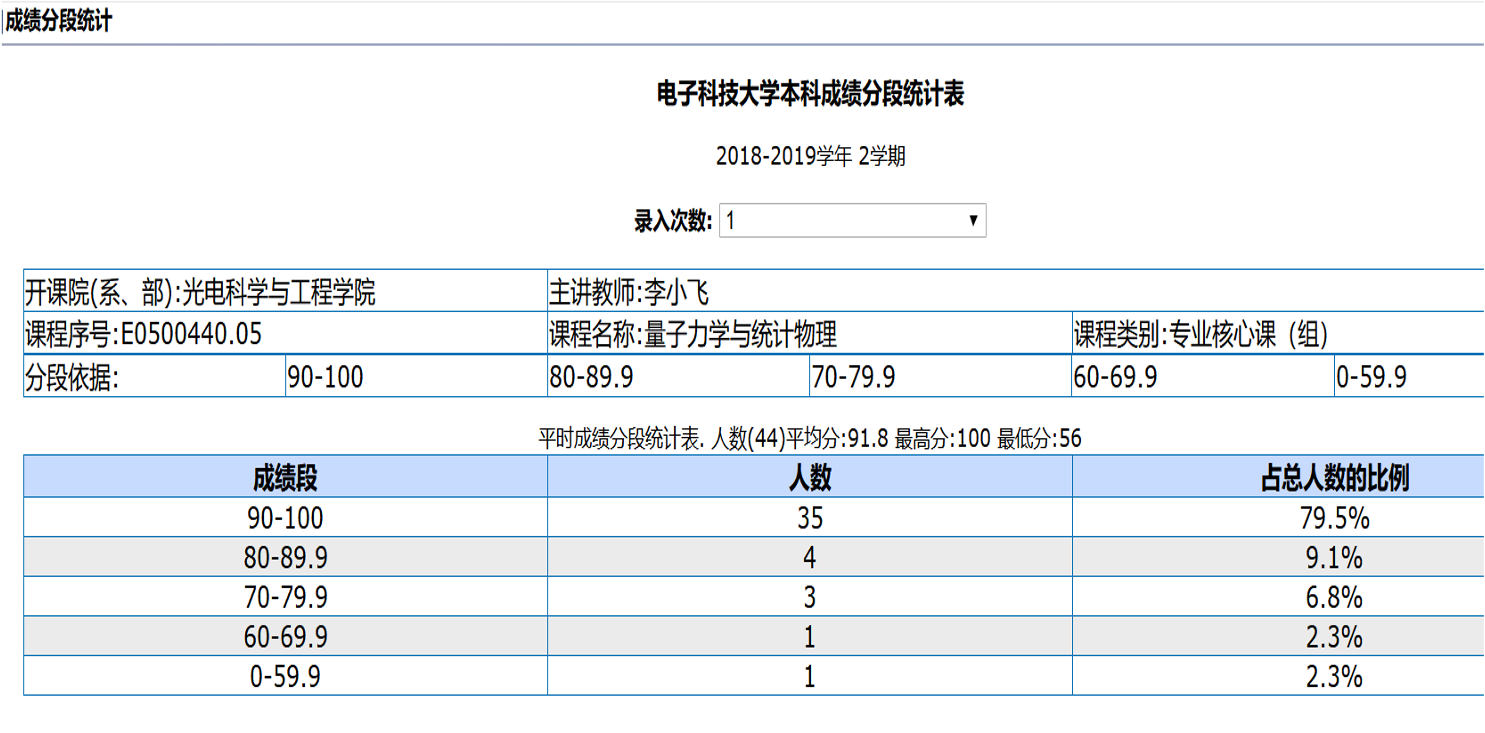
\includegraphics[width=1.0\textwidth,height=5.0cm]{figs/exam1.png}
\end{frame}

\begin{frame}
    \frametitle{参考书目}
        \begin{itemize}
            \Item 《量子力学》卷I,II, 曾谨言, 科学出版社, 2008           
            \Item Principles of quantum mechanics, shankar
            \Item Modern quantum mechanics, shankar
            \Item Lectures on quantum mechanics, weinberg
            \Item Principles of quantum mechanics, Dirac
        \end{itemize}
\end{frame}

\begin{frame}
    \begin{tcolorbox4}[三条军规]    
        \begin{enumerate}
            \Item Objects are wave-particles and can be in states of superposition
            \Item Rule 1 holds as long as you don't measure
            \Item Measurement gives random results
        \end{enumerate}
    \end{tcolorbox4} 
\end{frame}

\section{2.能量子假说}

\subsection{伟大成就}

\begin{frame}[t]
    \frametitle{经典物理伟大成就}
    \begin{tcolorbox3}
    [Great successes in Classical Physics]
        \begin{enumerate}
            \Item Newtonian mechanics
            \Item Maxwell's electromagnetism
            \Item Thermodynamic laws
        \end{enumerate}
    \end{tcolorbox3}  
    \begin{quotation}
        "There is nothing new to be discovered in physics now. All that remains is 
        more and more precise measurements"   \\
        \rightline{$\cdots$ Lord Kelvin (1900)\hspace{3em}}
    \end{quotation}
\end{frame}

\begin{frame}
    \frametitle{}
    \begin{quotation}
        "But the beauty and clearness ... is obscured by two small puzzling clouds \faCloud "  \\
        \rightline{$\cdots$ Lord Kelvin (1900.4)\hspace{3em}}   
    \end{quotation}
    ~~ \vspace{0.3em}
    \begin{tcolorbox4}[两朵乌云]    
        \begin{enumerate}
        \Item Michelson-Morley experiment
        \Item Black body radiation
        \end{enumerate}
    \end{tcolorbox4} 
\end{frame}

\begin{frame}
    \frametitle{迈克尔逊-莫雷实验}
    \begin{center}
    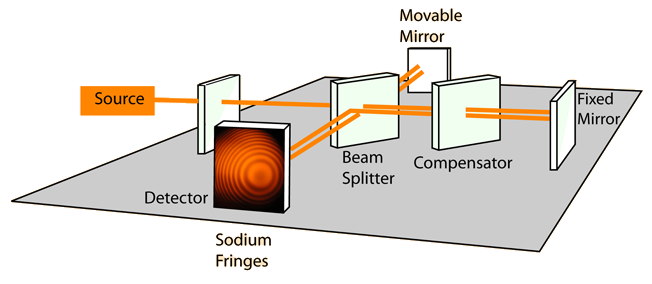
\includegraphics[width=0.8\textwidth]{figs/michel.png}
    \end{center}
There is no displacement of the interference bands. \dots 
the Stationary Ether is thus shown to be incorrect
\end{frame}

\begin{frame}
    The theory of relativity is established 
    \begin{center}
        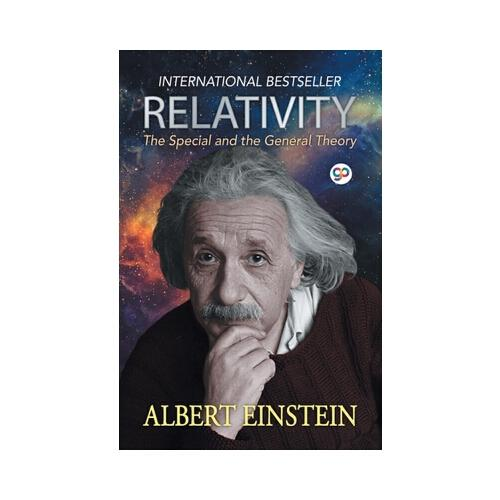
\includegraphics[width=0.4\textwidth]{figs/relativity.jpg}
    \end{center}   
    Greatly changed our view of time and space. Mainly useful in two aspects: high-speed motion, and strong gravitational field. 
\end{frame}

\begin{frame}
    \frametitle{黑体辐射实验}
    \begin{center}
    \includegraphics[width=0.7\textwidth]{figs/2021-12-01-23-47-27.png}
    \end{center}
    No mathematical function to describe the curves exactly 
\end{frame}
\begin{frame}
    Quantum mechanics is established  
    \begin{center}
        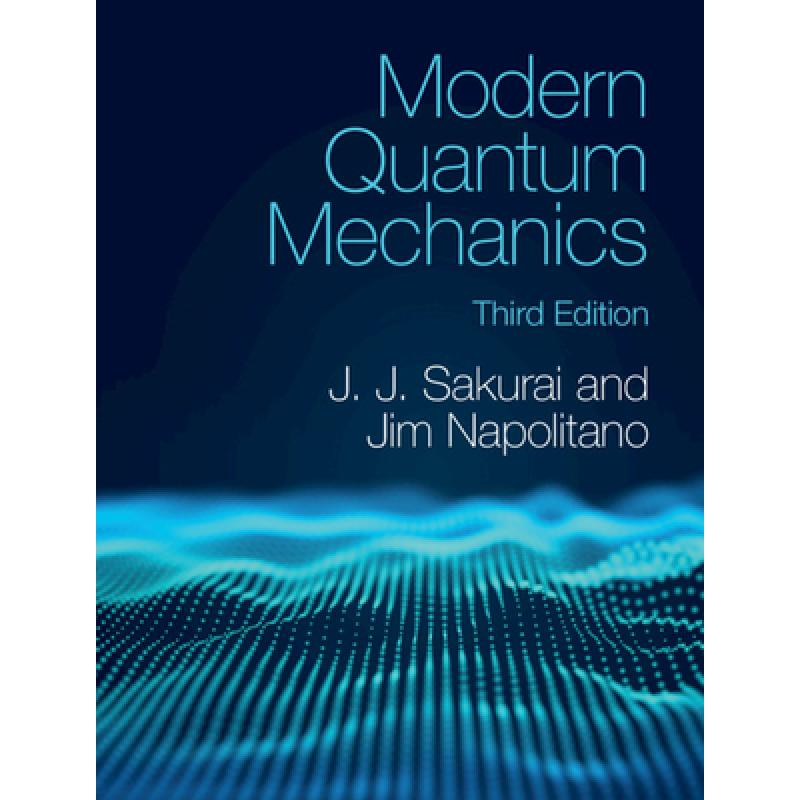
\includegraphics[width=0.45\textwidth]{figs/mqm.jpg}
    \end{center}   
    It is a theory about matter.
\end{frame}

\begin{frame}
    \frametitle{现代科学基石}
    \begin{center}
        \includegraphics[width=0.75\textwidth]{figs/stone.png}
    \end{center}   
\end{frame}

%%%%%%%%%%%%%%%%%%%%%%%%%%%%%%%%%%%%
\subsection{普朗克公式}
%%%%%%%%%%%%%%%%%%%%%%%%%%%%%%%%%%%%

\begin{frame}
    \frametitle{Black body radiation}
    \begin{definition}[Black body: ]
    \hspace{2em}absorb all electromagnetic waves in any temperature
    \end{definition}
    \begin{center}
        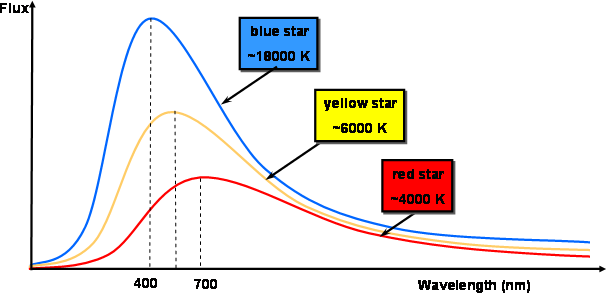
\includegraphics[width=0.55\textwidth]{figs/blackbody_radn_curves.png}
    \end{center}
    \textbf{\color{deepred} Most interestingly}, what is the mathematical function that describes all of these curves?
\end{frame}

\begin{frame}
    \frametitle{三个经验公式}
    \begin{center}
        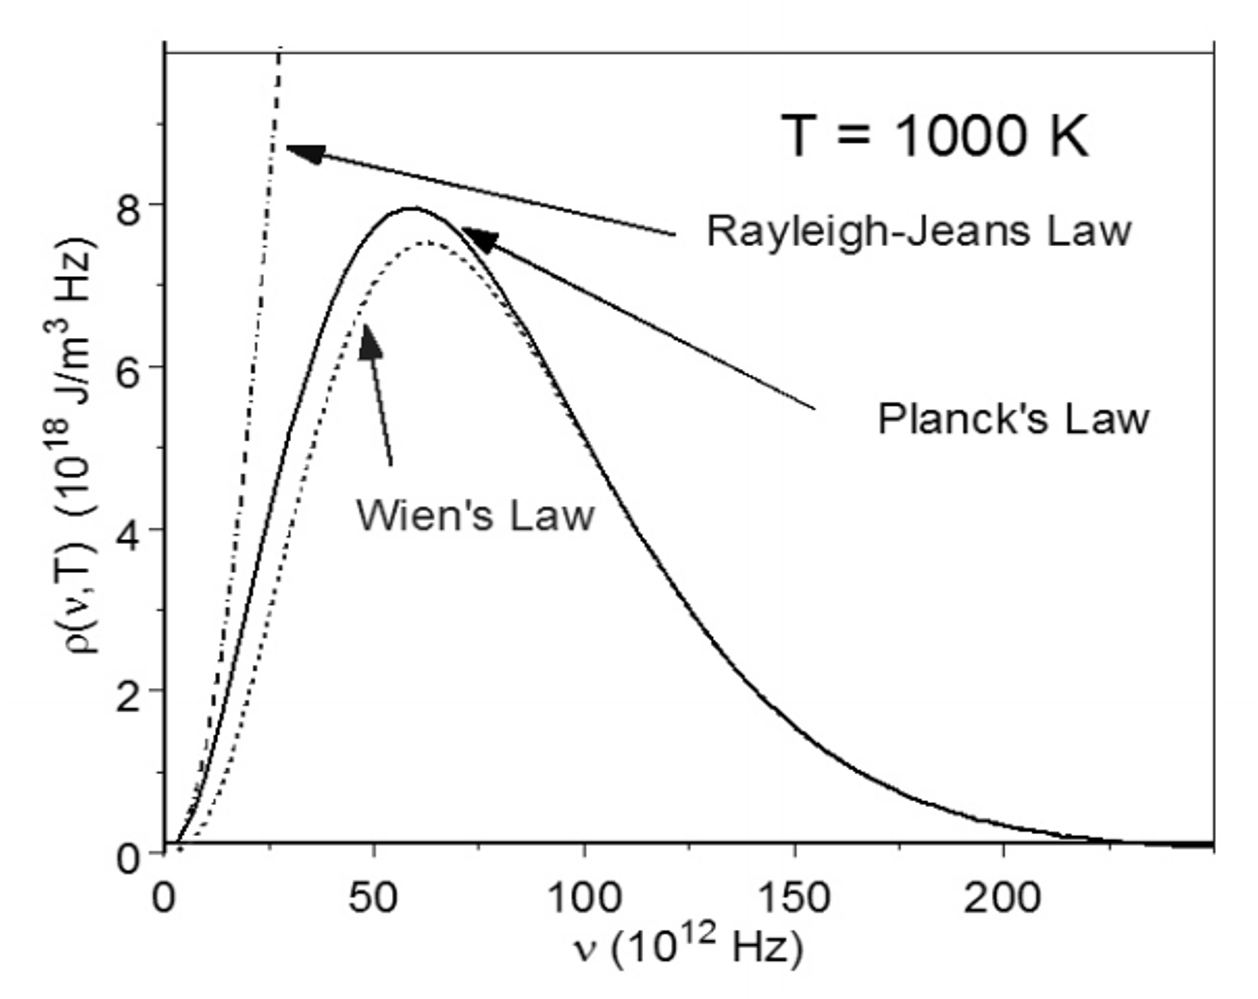
\includegraphics[width=0.7\textwidth]{figs/threelaws.png}
    \end{center}
\end{frame}

\begin{frame} [t]
    \frametitle{维恩公式}
    \begin{equation*}
        \rho(\nu) d \nu=c_{1} \nu^{3} e^{-c_{2} \nu / T} d \nu 
    \end{equation*}
    Derived from electromagnetism (1893), but described well only in high frequency region.\\ 
    {\color{deepred} Nobel Prize in physics(1911)}\\
\end{frame}

\begin{frame}[t]
    \frametitle{瑞-金公式}
    \begin{equation*}
        \rho(\nu, T) d \nu=\frac{8 \pi}{c^{3}} \nu^{2} k T d \nu 
    \end{equation*}
    Derived from thermodynamics (1900), but described well only in low frequency region.\\ 
   {\color{deepred} Nobel Prize in physics(1904)}\\ \vspace{0.3em}
   {\color{deepblue} {\Bullet} Ultraviolet Catastrophe:} 
    \begin{equation*}
         \int_0 ^\infty \frac{8 \pi}{c^{3}} \nu^{2} k T d \nu \to \infty 
    \end{equation*}
\end{frame}

\begin{frame}
    \frametitle{普朗克公式}
    On 1900-10-19, at the German Physical Society, 
    Max Planck presented a resolution to {\color{deepblue} Ultraviolet Catastrophe} 
    \begin{equation}
        \boxed{\rho(\nu, T) d \nu=\frac{8 \pi}{c^{3}} \frac{h \nu^{3}}{e^{h \nu / K T}-1} d \nu}
    \end{equation}
    Obtained from experimental data via interpolation technique, described well in whole region \\
    {\color{deepred} Nobel Prize in physics(1918)}\\
\end{frame}

\begin{frame}
    \centering
    \begin{tcbb}[0.7]{Problems}{
        How to derive the formula from existing theory.}
    \end{tcbb}
\end{frame}

\begin{frame}
    \begin{tcolorbox2}{Solution}
        On 1900-12-14, Planck gives out his solution based on the Energy Quantum Hypothesis  
    \end{tcolorbox2}
\end{frame}

%%%%%%%%%%%%%%%%%%%%%%%%%%%%%%%%%%%%
\subsection{能量子假说}
%%%%%%%%%%%%%%%%%%%%%%%%%%%%%%%%%%%%
\begin{frame}{能量子假说}
    \begin{tcolorbox4}[Energy quantum hypothesis]
    Assuming the oscillators of the cavity could only radiate at a discrete amounts of energy
    \begin{equation}
        E=n\varepsilon
    \end{equation}
    where, the $\varepsilon$ is the unit of the energy (quanta) determined by the oscillator' frequency 
    \begin{equation}
        \varepsilon=h\nu
    \end{equation}
    and the $h=6.6260693(11)\times10^{-34} J\cdot s,\quad (\hbar=\frac{h}{2\pi} \approx 6.58\times 10^{-16} eV\cdot s )$ is the Planck constant. 
    \end{tcolorbox4}
\end{frame}

\begin{frame} {推导公式}
    Based on Boltzmann distribution law,
    \begin{equation*}
        \frac{N_{i}}{N}=\frac{\exp \left(-\frac{E_{i}}{k T}\right)}{\sum_{i} \exp \left(\frac{-E_{i}}{k T}\right)}
    \end{equation*}
    {\Bullet} when the energy is continuous,the distribution between $E - dE$ should be 
    \begin{equation*}
        \frac{e^{-E / k T}}{\int\limits_{0}^{\infty} e^{-E / k T} d E}
    \end{equation*}  
    the average energy 
    \begin{equation*}
        <E>=\int\limits_{0}^{\infty} E \frac{e^{-E / k T}}{\int\limits_{0}^{\infty} e^{-E / k T} d E} d E
    \end{equation*}
\end{frame}

\begin{frame}
    \begin{equation*}
        \begin{split}
            <E> &= -kT \frac{Ee^{-E / k T}\vert_0 ^\infty-\int\limits_{0}^{\infty} e^{-E / k T} d E } {\int\limits_{0}^{\infty} e^{-E / k T} d E }\\  
                &= kT
        \end{split}  
    \end{equation*} 
    {\Bullet} when the energy is discrete,the distribution should be   
    \begin{equation*}
        \frac{e^{-E / k T}}{\int\limits_{0}^{\infty} e^{-E / k T} d E} 
        \to \frac{e^{-E / k T}}{\sum\limits_{0}^{\infty} e^{-E / k T}} 
        \to \frac{e^{-nh\nu / k T}}{\sum\limits_{0}^{\infty} e^{-nhv / k T}} 
    \end{equation*}    
\end{frame}

\begin{frame}
    the average energy 
    \begin{equation*}
        \begin{split}
            <E> &= \sum\limits_{0}^{\infty} nh\nu\frac{e^{-nh\nu / k T}}{\sum\limits_{0}^{\infty} e^{-nh\nu / k T}} \\
            &= -h\nu \frac{d}{dx} \frac{n e^{-nx}}{\sum\limits_{0}^{\infty} e^{-nx}} \\
            &= \frac{h\nu}{e^{h\nu/kT}-1} 
        \end{split} 
    \end{equation*}
    We get
    \begin{equation*}
        \text{(continuous)} \quad k T \rightarrow \frac{h \nu}{e^{ h \nu / k T}-1} \quad \text{(discrete)} 
    \end{equation*}
\end{frame}

\begin{frame}
    In Rayleigh-Jeans formula
    \begin{equation*}
        \rho(\nu, T) d \nu=\frac{8 \pi}{c^{3}} \nu^{2} k T d \nu 
    \end{equation*}
    the item $kT$ should be replaced by $\dfrac{h \nu}{e^{ h \nu / k T}-1}$
    \begin{equation*}
        \rho(\nu, T) d \nu=\frac{8 \pi}{c^{3}} \frac{h \nu^{3}}{e^{h \nu / K T}-1} d \nu
    \end{equation*}
    It is the Planck's formula exactly 
\end{frame}

\begin{frame}
    \begin{tcolorbox4}[Revolutionary Significance]
        Planck's Energy Quantum Hypothesis broke through the constraints of classical physics and 
        opened the door of quantum mechanics 
    \end{tcolorbox4}
\end{frame}

\begin{frame}
    \frametitle{}
    \centering
    \tcbb[0.68]{一只会下金蛋的鹅}
    {
    历史上,普朗克,德拜,艾伦菲斯特,劳厄,洛伦兹,庞加莱,泡利,玻色,爱因斯坦等从多角度推导过普朗克公式,每一次推导都给物理学带来了新的知识内容 
    }

 《黑体辐射公式的多种推导及其在近代物理构建中的意义》- 返朴|曹则贤
\end{frame}

%\begin{frame}
%    \begin{tcolorbox}[colback=yellow!10,colframe=red!75!black,title=THE END]
%    In 1927, Dirac got the Planck's formula from Quantum Mechanism.  
%    \end{tcolorbox}
%\end{frame}

\begin{frame}
    \frametitle{}
    \begin{tcolorbox3}[学术讨论]
        普朗克黑体辐射公式重要,还是能量量子化观念重要?\\
        能量量子化只是一种数学处理工具?
    \end{tcolorbox3}
\end{frame}

%%%%%%%%%%%%%%%%%%%%%%%%%%%%%%%%%%%%%%%%%%%%%%%%%%%%%%%%%%%%%%%%%%%
\begin{frame}
    \frametitle{作业}
   \begin{enumerate}
       \item Planck's Energy Quantum Hypothesis
       \item What's the quanta
       \item Deriving the Rayleigh-Jeans formula and Wien's formula from Planck's formula
   \end{enumerate}
\end{frame}
%%%%%%%%%%%%%%%%%%%%%%%%%%%%%%%%%%%%%%%%%%%%%%%%%%%%%%%%%%%%%%%%%%%

\section{3.波粒二象性}      

\begin{frame}
    \frametitle{}
    \begin{tcolorbox3}[前情回顾]
        Assuming the oscillators can radiate at a discrete amounts of energy
        \[    E=n\varepsilon, \qquad (n=1,2,3,\cdots) \]
        and the unit of the energy is determined by the oscillator' frequency
        \[   \varepsilon=h\nu  \]
        one can derive the framula:
        \[ \rho(\nu, T) d \nu=\frac{8 \pi}{c^{3}} \frac{h \nu^{3} }{e^{h \nu / K T}-1} d \nu \]
    \end{tcolorbox3}
\end{frame}

\begin{frame}
    \frametitle{粒-波的不可调和性}
	\begin{columns}
		\begin{column}[t]{0.46\linewidth}
			粒子性
			\begin{itemize}
				\Item  确定的位置、能量、动量等
				\Item  两个粒子不能同时占据同一位置
				\Item  同一粒子也不能同时占据多个位置
				\Item  碰撞现象
			\end{itemize}
		\end{column}
		\begin{column}[t]{0.46\linewidth}
			波动性
			\vspace{1ex}
			\begin{itemize}
				\Item  确定的波长、振幅、相位等
				\Item  可以同时出现在同一位置
				\Item  可以同时占据多个位置
				\Item  衍射、干涉,无碰撞
			\end{itemize}
		\end{column}
	\end{columns}
\end{frame}

\begin{frame} 
    人们通过上述特性进行判定\\
    \begin{itemize}
        \Item  一个物体要么是粒子,要么是波
        \Item  这个方法一直是有效
        \Item  直到遇到**光** 
    \end{itemize}   
    \begin{figure}
        \centering
        \subfigure[]{\includegraphics[width=7.4cm]{figs/2021-12-02-15-26-40.png}}
        \subfigure[]{
\includegraphics[width=4.5cm]{figs/2021-12-06-11-44-50.png}}
        %\caption{} %图片标题
        %\label{fig:1}  
    \end{figure} 
    \setcounter{subfigure}{0}
\end{frame}

\begin{frame}
	\begin{columns}
		\begin{column}[t]{0.46\linewidth}
            水波
            \begin{center}
                \includegraphics[width=2.5in,height=2.5in]{figs/2021-12-02-15-46-16.png}
            \end{center}
		\end{column}
		\begin{column}[t]{0.46\linewidth}
            光波
            \begin{center}
                \includegraphics[width=2.5in,height=2.5in]{figs/2021-12-02-15-49-36.png}
            \end{center}
		\end{column}
	\end{columns}
\end{frame}

\begin{frame} {光的波动说}
    \begin{center}
        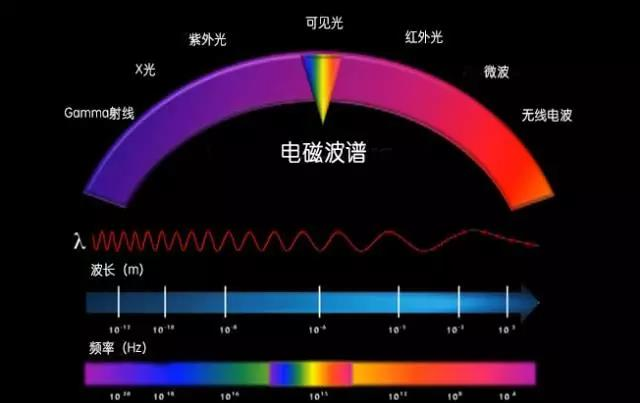
\includegraphics[width=0.70\textwidth]{figs/2021-12-02-16-23-16.png}
    \end{center}
    光只是一定波长范围内的电磁波
\end{frame}

\begin{frame} 
    波动说面临的困难:
    \begin{itemize}
        \Item  黑体辐射
        \Item  光电效应
        \Item  康普顿效应
        \Item  氢原子光谱
    \end{itemize}
\end{frame}

%%%%%%%%%%%%%%%%%%%%%%%%%%%%%%%%%%%%
\subsection{光电效应}
%%%%%%%%%%%%%%%%%%%%%%%%%%%%%%%%%%%%

\begin{frame} 
    \frametitle{光电效应实验}   
    \begin{center}
       \includegraphics[width=0.53\textwidth]{figs/2021-12-02-16-01-21.png}
   \end{center}  
   {\Bullet} 具有瞬时性 \\
   {\Bullet} 存在临界频率 $\nu_0$ \\
   {\Bullet} 光电子能量由光的频率决定
\end{frame}  

\begin{frame} 
    In 1905, Einstein considered the derivation of Planck's Law  \\
    \begin{itemize}
        \Item  Plank’s Law was consistent with experment but not with existing theory
        \Item  Rayleigh-Jeans Law was consistent with existing theory but not with experiment
        \Item  For treating Ultraviolet Catastrophe, he proposed the light quantum hypothesis
        \Item  Using light quantum hypothesis, he explained the Photoelectric effect
    \end{itemize}
\end{frame}

\begin{frame}
    \frametitle{}
        \begin{figure}
            \centering
            \subfigure[光强分布]{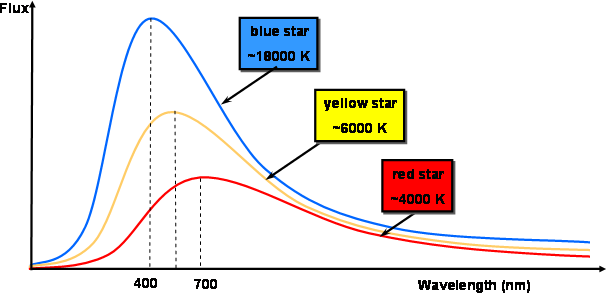
\includegraphics[width=0.495\textwidth]{figs/blackbody_radn_curves.png}}
            \subfigure[粒子数分布]{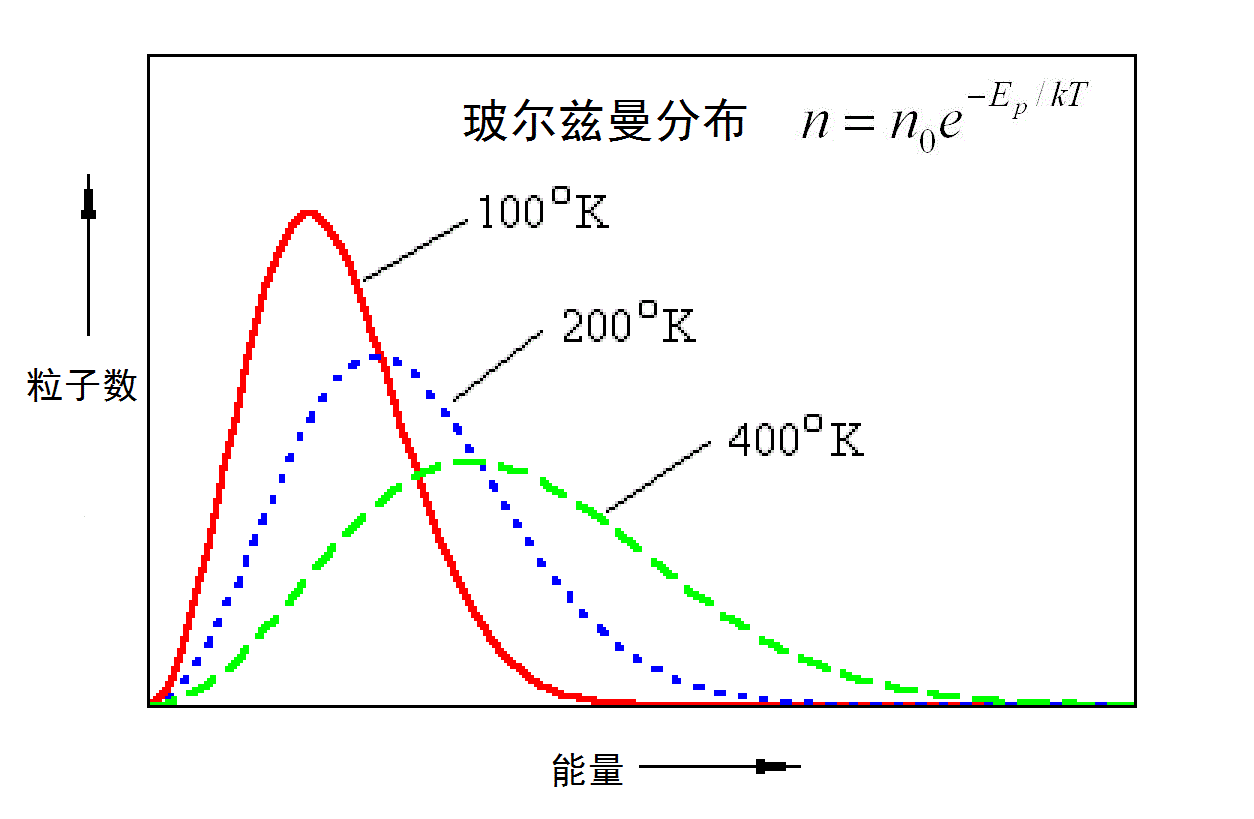
\includegraphics[width=0.495\textwidth]{figs/2022-01-17-14-21-43.png}}
        \end{figure}
    \setcounter{subfigure}{0}
\end{frame}

\begin{frame} 
    \begin{tcolorbox4}[Light quantum hypothesis]
        {\Bullet} Light likes particles with unit energy  (quanta).\\
        \[E=h\nu\]  
        {\Bullet} The energy of n light quantum is $nh\nu$. \\
        {\Bullet} The momentum of light quantum is (1918) \\
        \[p=\frac{E}{c}=\frac{h\nu}{c}=\frac{h}{\lambda}\]
    \end{tcolorbox4}
\end{frame}

\begin{frame} 
    基于光量子假说,提出光电效应公式
    \[
    \frac{1}{2}m_eV_0^2=h\nu-W
    \]
    \begin{itemize}
        \Item  瞬时性:光如果是粒子,碰上电子则能量被瞬时吸收
        \Item  临界频率:$\nu_0=\frac{W}{h} $
        \Item  光电子能量与光的频率决定: $E_k=h\nu-W$
    \end{itemize}
    {\color{deepred} Nobel Prize in physics(1921)}
\end{frame}

\begin{frame} 
    基于光电效应公式:
$$
\frac{1}{2}m_eV_0^2=h\nu-W
$$
1916年,密立根实验上测定普朗克系数,验证光子说\\
\color{deepred}{1923年诺贝尔物理学奖} 
\end{frame}

\begin{frame} 
    \begin{tcolorbox4}[光量子假说的意义]
        \begin{itemize}
            \Item  揭示能量子的本质:在于光本身是量子化的,具有粒子性
            \Item  揭示光的本质:光既具波动性又具粒子性。
        \end{itemize}
    \end{tcolorbox4}
    \begin{quotation}
        "在近代物理学结出硕果的那些重大问题中,很难找到一个问题是爱因斯坦没有做出过重要贡献的。
        在他的各种推测中,他有时可能也曾经没有中标的,例如他的光量子假设,就有点迷失了方向\dots"  \\
        \rightline{$\cdots$ 普朗克\hspace{3em}}   
    \end{quotation}
\end{frame}

%%%%%%%%%%%%%%%%%%%%%%%%%%%
\subsection{康普顿效应}
%%%%%%%%%%%%%%%%%%%%%%%%%%%

\begin{frame}   
    \frametitle{康普顿效应 (1922)}
    \begin{center}
        \includegraphics[width=0.7\textwidth, height=3in]{figs/comptonscattering.png}
    \end{center}  
\end{frame}

\begin{frame} 
    ~~\\ 
    经验公式:$\lambda_{out}-\lambda_{in}=\lambda_e(1-\cos \theta)$ \\  \vspace*{0.6em}
    \alert{解:} Energy of electron 
    \begin{equation*}
        E^2 =m_ec^2=p^2c^2 +m_0 ^2 c^4 
    \end{equation*}
    Energy of light quantum
    \begin{equation*}
        E =pc 
    \end{equation*}
    energy conservation law
    \begin{equation*}
        \begin{split}
        E_i + m_0 c^2 &= E_o + m_ec^2 \\
        (E_i -E_o + m_0 c^2)^2 &= E_e ^2\\
        (p_i c-p_o c + m_0 c^2) ^2 &= p_e ^2 c^2 +m_0 ^2 c^4 \\
        (p_i-p_o)^2 +2 m_0 (p_i c-p_o c) &= p_e ^2
    \end{split}
    \end{equation*}
\end{frame}

\begin{frame}  
    momentum conservation law
    \begin{equation*}
        \begin{split}
            \vec{p}_i -\vec{p}_o &= \vec{p}_e \\
            (\vec{p}_i -\vec{p}_o)\cdot (\vec{p}_i -\vec{p}_o)  &= \vec{p}_e\cdot \vec{p}_e   \\
            p_i ^2 + p_o ^2 -2p_i p_o \cos \theta &= p_e ^2  \\
            p_i ^2 + p_o ^2 -2p_i p_o \cos \theta &= (p_i-p_o)^2 +2 m_0 (p_i c-p_o c) \\
            \frac{1}{p_o} -\frac{1}{p_i} &= \frac{1}{m_0 c} (1-\cos \theta) \\
            \lambda_o -\lambda_i &= \frac{h}{m_0 c} (1-\cos \theta) 
        \end{split}
    \end{equation*}
\end{frame}

\begin{frame}   
    \begin{tcolorbox3}[Significance]
        Prove that:\\
        {\Bullet} The light of wavelength ($\lambda$) possesses a quantum momentum \[p=\frac{h}{\lambda}\]
        {\Bullet} Momentum conservation law works in subatom scales 
    \end{tcolorbox3}   
    \color{deepred}{Nobel Prize in physics(1927)}\\
\end{frame}

%%%%%%%%%%%%%%%%%%%%%%%%%%
\subsection{氢原子光谱}
%%%%%%%%%%%%%%%%%%%%%%%%%%

\begin{frame}  
     \frametitle{氢原子光谱}
     \begin{center}
        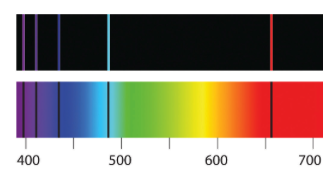
\includegraphics[width=0.6\textwidth]{figs/2022-01-17-14-02-45.png}
    \end{center}  
    经验公式:
       $\dfrac{1}{\lambda}=R_H c (\dfrac{1}{m^2} -\dfrac{1}{n^2})$ \\ \vspace{0.3em}
    \alert{Problem:} the formula cannot be derived from existing theory
\end{frame}

\begin{frame} 
    \frametitle{Rutherford model}  
    \begin{center}
        \includegraphics[width=0.8\textwidth]{figs/utherford_atom.png}
    \end{center}  
\end{frame}

\begin{frame}  
    \begin{tcolorbox4}[Bohr's hydrogen atom hypothesis]
    Bohr asummed that :\\
    {\Bullet} Stationary states: Electrons move around the nucleus only in certain allowed circular orbits with fixed energy \\
    \[ L=n \frac{h}{2\pi}= n \hbar,\qquad (\oint p_i dq_i = n_i h)\]
    {\Bullet} Quantum transition: Electron can jump between stationary state orbits when absorbed or emitted a photon with certain energy\\
    \[ h\nu=E_n -E_m \]
    \end{tcolorbox4}
\end{frame}

\begin{frame}   
    \frametitle{}
    推导光谱公式\\
    {\Bullet} Stationary state orbit radius:
    \begin{equation*}
        \begin{split}
            m\frac{v^2}{r}&=\frac{1}{4\pi\epsilon_0} \frac{e^2}{r^2} \\
            L=&mvr =n\hbar \\
            r_n&= n^2 (\frac{\epsilon_0 h^2}{m\pi e^2}) =n^2 r_1   
        \end{split} 
     \end{equation*}
     {\Bullet} Stationary state orbit energy: 
     \begin{equation*}
        \begin{split}
            E_n &= T + U \\
            &= \frac{1}{2}mv^2- \frac{1}{4\pi\epsilon_0} \frac{e^2}{r_n ^2} \\
            &= \frac{1}{n^2} (-\frac{m e^4}{8 \epsilon_0 ^2 h^2}) = \frac{E_1}{n^2}
        \end{split}  
     \end{equation*}
\end{frame}

\begin{frame}
    {\Bullet} Spectrum formula: 
    \begin{equation*}
        \begin{split}
         \nu&=\frac{E_n -E_m}{h} \\
         &= \frac{m e^4}{4\pi \hbar ^3} [\frac{1}{m^2} -\frac{1}{n^2}]
        \end{split}  
     \end{equation*}
     {\Bullet} Rydberg constant : 
     \[R_{theo}= \frac{m e^4}{4\pi \hbar ^3 c} =1.0973731\times 10^7 m^{-1}\]
    \[R_{exp}=1.0974\times10^7 m^{-1} \]  
\end{frame}

\begin{frame}   
    \frametitle{Bohr's model}  
    \begin{center}
        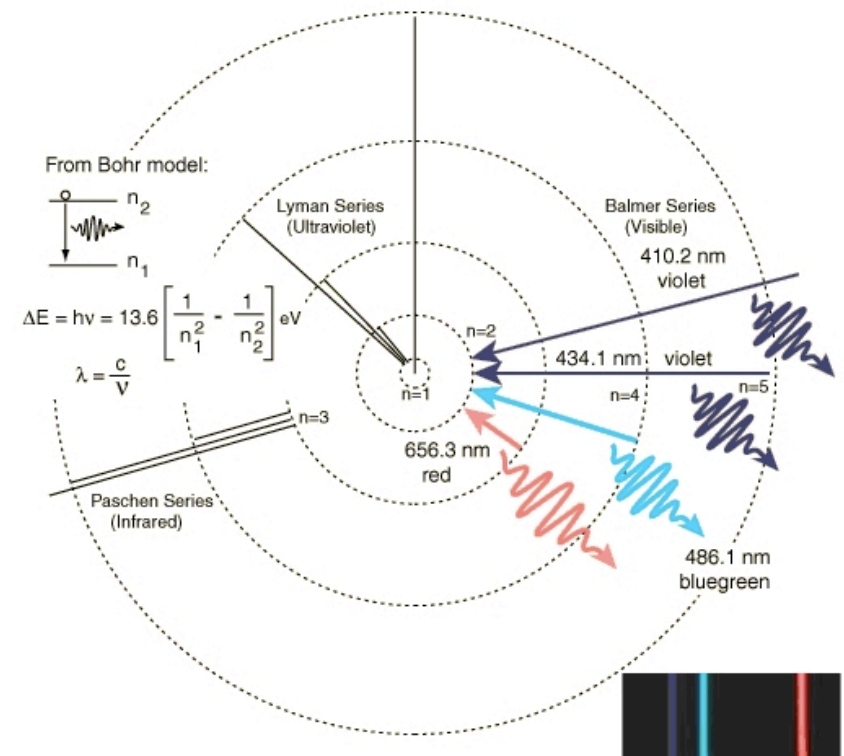
\includegraphics[width=0.6\textwidth]{figs/bohrmodel.png}
    \end{center}  
    {\Bullet} 1905年爱因斯坦提出的光子概念,不受名人的重视,普朗克把爱因斯坦的光量子概念说成是“迷失了方向”。\\
    {\Bullet} 1913年,28岁的玻尔,创造性地把光子概念用到卢瑟福模型上,成功破解氢原子光谱问题 \\
    {\color{deepred} {\Bullet} Nobel Prize in physics(1922)}\\ 
\end{frame}

\subsection{光的波粒二象性} 

\begin{frame} 
  \frametitle{光的波粒二象性}  
  {\Bullet} In 1905, when Einstein first put forward this hypothesis, 
  he simply stated that light consisted of quanta with energy \[ E = h\nu \] 
  {\Bullet} In 1917, he stated that the light quantum carried a momentum of  \[ p=\frac{h}{\lambda}\]
  At this point, the light quantum with massless particle property was named as photon (光子)
\end{frame}

\begin{frame}  
  $\begin{cases}
    \text{Light behaves like waves }\\
    \text{~~\qquad Interference} \\
    \text{~~\qquad Diffraction} \\
    \text{Light behaves like particles}\\
    \text{~~\qquad Black body radiation} \\
    \text{~~\qquad Photoelectric effect} \\
    \text{~~\qquad Compton effect} \\
   \end{cases}$\\
   ~~\\
   Light has both wave and particle properties is called \alert{wave-particle duality} of light
\end{frame}

\begin{frame}
    \frametitle{}
    \begin{tcolorbox3}[学术讨论]
        ~\\
        How can the light be both particle and wave ?
    \end{tcolorbox3}
\end{frame}

%%%%%%%%%%%%%%%%%%%%%%%%%%%
\subsection{物质波假说}
%%%%%%%%%%%%%%%%%%%%%%%%%%%

\begin{frame}   
  \frametitle{物质波假说}
  \begin{tcolorbox4}[Matter wave hypothesis]
  In 1923, de Broglie states that if light which is classically a wave could behave as a particle
  then classical particles could also behave as quantum waves. The wave length and frequency are
  \[\lambda=\frac{h}{p}\]
  \[\nu =\frac{E}{h}\]
  \end{tcolorbox4}
\end{frame}

\begin{frame}  
    \frame{}
    Calculating de Broglie wavelength of electron in Bohr's H atom model
    \begin{equation*}
        \begin{split}
            L&=n\hbar \\
            \vec{r} \cdot \vec{p} & =  n\frac{h}{2 \pi} \\
            2\pi r&=  n\frac{h}{p}\\
            2\pi r&=  n\lambda 
        \end{split} 
     \end{equation*}
     Now, we called it standing-wave condition 
\end{frame}


\begin{frame}   
  \frametitle{Experimental verification}
  \begin{center}
    \includegraphics[width=0.5\textwidth]{figs/elediffr.jpeg} \\
    Electron diffraction patterns (Davisson and Germer, 1927)
    \end{center} 
\end{frame}
\begin{frame}   
    \begin{center}
      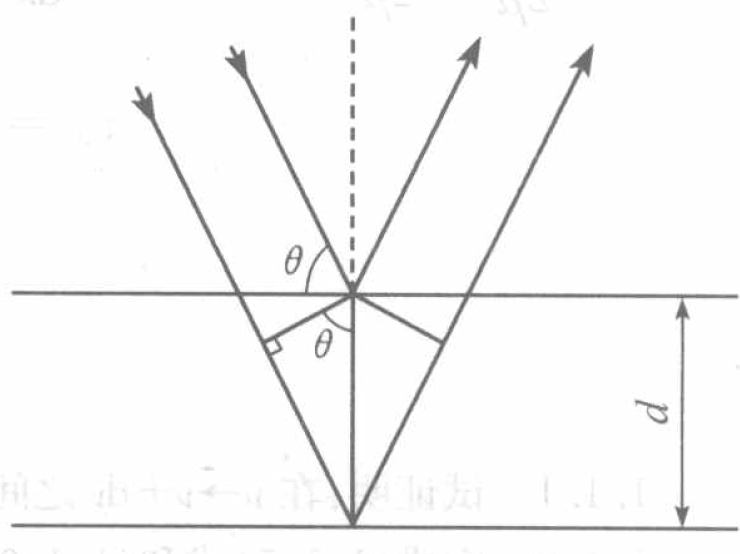
\includegraphics[width=0.55\textwidth]{figs/scatting.png} \\
    \end{center} 
    \begin{itemize}
        \Item  Meeting Bragg formula $2d\sin \theta=n\lambda $
        \Item  Obtaining the wavelength of electron (about 0.16X $nm$), agreeing well with the 
   calculated de Broglie wavelength 
    \end{itemize}
  {\color{deepred} Nobel Prize in physics(1937)}  
  \end{frame}

  \begin{frame}
      \frametitle{}
    \begin{center}
         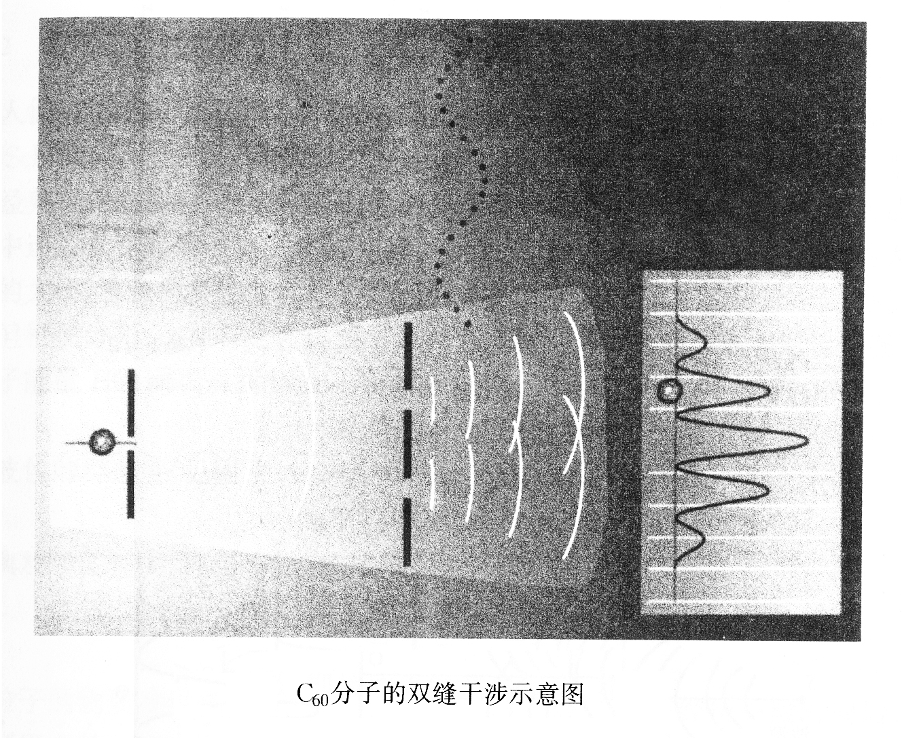
\includegraphics[width=0.8\textwidth,height=2.5in]{figs/c60.png}
    \end{center}
  \end{frame}
\begin{frame} 
    \begin{tcolorbox}[colback=yellow!10,colframe=red!75!black,title=Significance]
        De Broglie extended the wave-particle duality from light to particles! \\
        {\color{deepred} Nobel Prize in physics(1929)} for discovery of wave nature of electrons
    \end{tcolorbox}  
\end{frame}

\begin{frame}{电子双缝干涉实验}
    \includemedia[
    width=1.0\linewidth,height=0.67\linewidth, % 16:9
    activate=pageopen,
    addresource=figs/doubleslite-n.mp4,
    flashvars={
    source=figs/doubleslite-n.mp4
    &autoPlay=true % start playing on activation
    &loop=true
    }
    ]{}{VPlayer.swf}
\end{frame}

\begin{frame}
    \frametitle{学术讨论}
        \begin{figure}
            \centering
            \subfigure[]{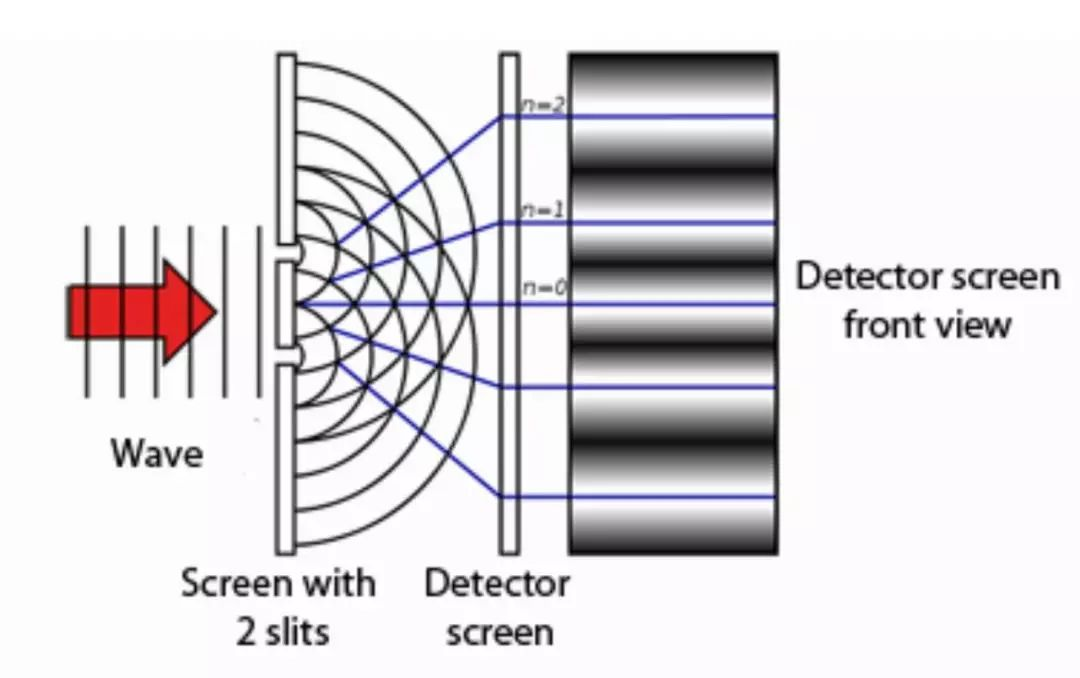
\includegraphics[width=4.5cm]{figs/ds-1.jpeg}}
            \subfigure[]{\includegraphics[width=4.5cm]{figs/ds-2.jpeg}}
            \subfigure[]{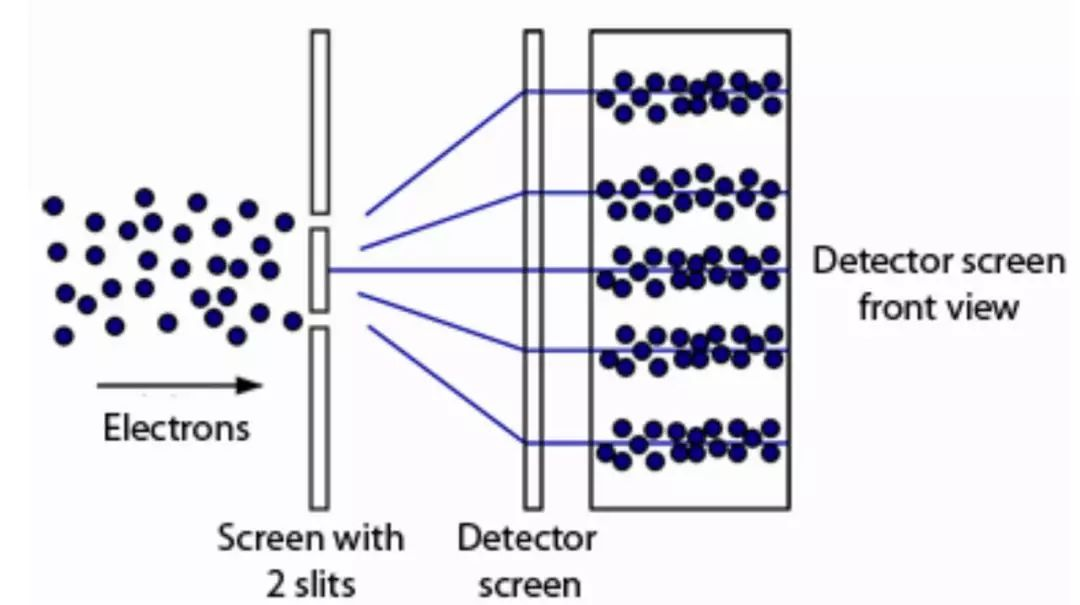
\includegraphics[width=4.5cm]{figs/ds-3.jpeg}}
            %\caption{} %图片标题
            %\label{fig:1}  
            {\color{red} How can electrons be both a particle and a wave?}
        \end{figure}
    \setcounter{subfigure}{0}
\end{frame}

\begin{frame}  
    \begin{tcolorbox3}[Conclusion]
    Wave-particle duality is the inherent attribute of matter
    \end{tcolorbox3} 
\end{frame} 

\begin{frame}
    \frametitle{}
    \centering
    \tcbb[0.5]{Big problems}
    {
      \large  How to interpret a world where waves are particles and particles are waves
    }
\end{frame}

%%%%%%%%%%%%%%%%%%%%%%%%%%%%%%%%%%%%%%%%%%%%%%%%%%%%%%%%%%%%%%%%%%%
\begin{frame}
    \frametitle{课外作业}
    \begin{enumerate}
        \item 计算氢原子第一玻尔半径上电子的德布罗意波长
        \item 计算经 50 V 电势装成加速后电子的德布罗意波长
    \end{enumerate}
\end{frame}
%%%%%%%%%%%%%%%%%%%%%%%%%%%%%%%%%%%%%%%%%%%%%%%%%%%%%%%%%%%%%%%%%%%  
%%%%%%%%%%%%%%%%%%%%%%%%%%%%%%%%%%%%%%%%%%%%%%%%%
	\begin{frame}
		\frametitle{}
		\Background[1] 
	    \begin{center}
		{ {\Huge 第二章~~三大偏微分方程\\(6学时)}}
	    \end{center}    
	\end{frame}
%%%%%%%%%%%%%%%%%%%%%%%%%%%%%%%%%%%%%%%%%%%%%

\begin{frame}
	\frametitle{}
	\begin{definition}[] 
	偏微分方程(PDE)指未知函数是多元函数的微分方程,
	方程的函数(物理量)多以时间和空间为变量,这些方程的来源和应用通常具有物理学背景。又称为数学物理方程。
	\end{definition}
	方程的最高阶是二阶的称为二阶偏微分方程
	\begin{equation*}
		au_{xx}+2bu_{xy}+cu_{yy}+du_x+eu_y+fu=g
	\end{equation*}
	根据$\Delta=b^2-ac$二阶偏微分方程可分为三类:椭圆型($\Delta<0$)、双曲型($\Delta>0$)和 抛物型 ($\Delta=0$),\\
	它们的代表分别是:拉普拉斯(泊松方程)、波动方程、热传导方程
\end{frame}

\begin{frame}
\frametitle{三大偏微分方程}
	\begin{itemize}
	\item  波动方程 
	\begin{equation*}
		u_{tt}=a^2u_{xx}
	\end{equation*}
	\item  热传导方程
	\begin{equation*}
		u_t=a^2 \nabla ^2 u 
	\end{equation*}
	\item  拉普拉斯方程
	\begin{equation*}
		 \nabla ^2 u =0
	\end{equation*}
	\end{itemize}
\end{frame}

%%%%%%%%%%%%%%%%%%%%%%%%%%%%%%%%%%%%%%%%%%%%%
\section{1.波动方程}
\subsection{方程的建立}
\begin{frame}
	\frametitle{方程的建立}	
	\begin{exampleblock} {例1、	求弦振动方程}
	考虑均匀柔软的细弦线,二端固定,受到扰动后在平衡位置作微小运动。分析位移函数 u(x,t)满足的方程。\\
	\centering
	\begin{tikzpicture}
	%\draw[eaxis] (0,0) -- (8,0) node[below] {$x$};
	%\draw[eaxis] (0,0) -- (0,0.5) node[right] {$y$};
	\draw (0,0) .. controls (2, 1) and (6,1) .. (8,0);
	\filldraw[red] (0,0) circle [radius=1pt];
	\filldraw[red] (8,0) circle [radius=1pt];
	\end{tikzpicture}
	\end{exampleblock} 	
	自然界普遍存在各种振动,振动的传播形成波,服从统一的方程。	
\end{frame}	

\begin{frame}
	\frametitle{}	
	\begin{center}
		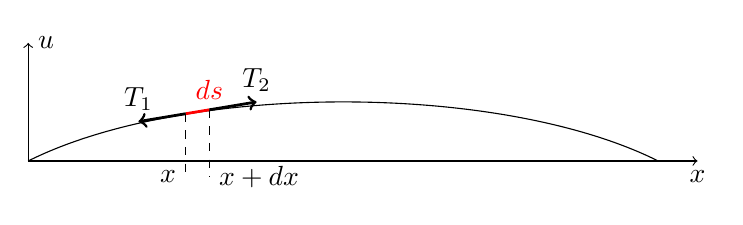
\begin{tikzpicture}
		\draw[->] (0,0) -- (8.5,0) node[below] {$x$};
		\draw[->] (0,0) -- (0,1.5) node[right] {$u$};
		\draw (0,0) .. controls (2, 1) and (6,1) .. (8,0);
		%	\filldraw[red](2,0.6)circle[radius=1pt];
		\draw[dashed] (2,0.6) --(2,-0.2) node[left] {$x$}; 
		%	\filldraw[red](2.3,0.65)circle[radius=1pt];
		\draw[dashed] (2.3,0.65) --(2.3,-0.2) node[right] {$x+dx$}; 
		\draw[red,  line width =1pt] (2,0.6) --(2.3,0.65) node[above] {$ds$};  
		\draw[->, line width =1pt] (2,0.6) --(1.4,0.5) node[above] {$T_1$};  
		\draw[ ->,  line width =1pt] (2.3,0.65) --(2.9,0.75) node[above] {$T_2$};  
	\end{tikzpicture}\\	 \vspace{0.3 em}
	\end{center}
	\alert{解:} 建立坐标系,  取任意微元ds, 临近拉力$T_1, T_2$:\\
	水平:{ $T_2\cos \alpha _2=T_1\cos \alpha _1=T_0$ }  \\   
	竖直:{$T_2\sin \alpha _2-T_1\sin \alpha _1=ma=\rho ds~ u_{tt} $}   \\   
	有~:{ $T_0(\tan \alpha _2-\tan \alpha _1)=\rho ds ~u_{tt}$ }   \\   \vspace{0.3 em}
    \hspace{1cm}$T_0[u_x(x+dx,t)-u_x(x,t)]=\rho dx ~u_{tt}$  \\   \vspace{0.6 em}
	\hspace{1cm}$\displaystyle \frac{T_0}{\rho}\times\frac{u_x(x+dx,t)-u_x(x,t)}{dx}=u_{tt}$ \\ \vspace{0.3 em}
	\Tips (1)斜率就是一阶导,(2)小角度条件下,$ds \simeq dx$
\end{frame}	

\begin{frame}
	\frametitle{}	
	得波动方程:
	\begin{equation*}
		u_{tt}=a^2u_{xx}
	\end{equation*}
	定解条件:\\
	(1) 初始条件 
	$\displaystyle  u(x,t)|_{t=0}= \psi (x) $, 	 $\displaystyle  u_t(x,t)|_{t=0}= \Psi (x) $\\
	(2) 边界条件
	$\displaystyle  u(x,t)|_{x=0}= 0 $, 	 $\displaystyle  u(x,t)|_{x=l}= 0 $\\ 	\vspace{0.3cm} 
	若质点受外力作用, 有:
	\begin{equation*}
		u_{tt}=a^2u_{xx} +f(x,t)
	\end{equation*}
	\begin{block} {Remark}
		波动方程描述了围绕平衡态小幅震荡的规律,它不仅可描述琴弦、鼓膜、耳机的震动,也描述着光波、声波、地震波、引力波,甚至弦论中弦的运动。
	\end{block}
\end{frame}	
%%%%%%%%%%%%%%%%%%%%
\subsection{方程的求解}
\begin{frame}
	\frametitle{方程的求解}	
	\begin{exampleblock} {例2、	求一维波动方程}
	$\displaystyle \begin{cases}
		u_{tt}=a^2u_{xx}\\
		u(x,t)|_{t=0}= \psi (x) ,~~~ u_t(x,t)|_{t=0}= \Psi (x) \\
		u(x,t)|_{x=0}= 0, ~~~  u(x,t)|_{x=l}= 0 
	\end{cases}$ \\	
	\end{exampleblock} %2
	\alert{解:} 	(傅里叶)   设 $\displaystyle  u(x,t)=T(t)X(x) $,代回方程 , 得:
	\begin{equation*}
		 T~^{''}(t)X(x) =a~^2 T(t)X~^{''}(x) 
	\end{equation*}
	 \hspace{1cm} 可分离变量
\end{frame}	

\begin{frame}
	\frametitle{}	
	$ \dfrac{T~^{''}}{a~^2 T}=\dfrac{X~^{''} }{X} =-\lambda $ \\ \vspace{0.3cm}
	转化为两常微分方程 \\ \vspace{0.3cm}
	方程(I):
	$\displaystyle  \begin{cases}
		X~^{''} +\lambda X=0  ~~,~~ 0<x<l\\
		X(0)=0 ~,~X(l)=0
	\end{cases}$ \\	
	方程(II):
	$\displaystyle  \begin{cases}
		T~^{''} +\lambda {a~^2 T}=0 \\
		......
	\end{cases}$ \\	
	\begin{block} {Remark}
		偏微分方程与常微分方程的分离变量法有何不同?
	\end{block}
\end{frame}	

\begin{frame}
	\frametitle{}	
	解方程(I):有特征(辅助)方程, 
	\begin{equation*}
		\mu~^2 +\lambda =0
	\end{equation*}
	根为:
	$\displaystyle  \begin{cases}
		\mu~_1=+\sqrt{-\lambda}\\
		\mu~_2=-\sqrt{-\lambda}
	\end{cases}$ \\	\vspace{0.6 em}	
	{\Bullet}~分情况讨论:\\
	(1) 相异实根($\lambda < 0$)
	有通解:	{ $\displaystyle 	X=Aexp~^{\sqrt{-\lambda}x} + Bexp~^{-\sqrt{-\lambda}x} $ } \\ 
	分别取$x=0, x=l$, 得定解方程组:\\
	$\left[
	\begin{array}{lll}
		1&1\\
		exp~^{\sqrt{-\lambda}~l} &exp~^{-\sqrt{-\lambda}~l}
	\end{array}
	\right]$
	$\left[
	\begin{array}{ll}
		A\\
		B
	\end{array}
	\right]$
	=$\left[
	\begin{array}{ll}
		0\\
		0
	\end{array}
	\right]$
\end{frame}	

\begin{frame}
\frametitle{}	
	有解条件为:
	$\begin{vmatrix}
		1&1\\
		exp~^{\sqrt{-\lambda}~l} &exp~^{-\sqrt{-\lambda}~l}
	\end{vmatrix}
	= 0$\\
	很明显,这个行列式不等于0, 所以只有零解 (A=0,~B=0)    \\ \vspace{0.3cm}
	(2) 相同实根($\lambda = 0$),\\
	则通解为:	{ $\displaystyle 	X=Ax + B $ } \\ 
	分别取$x=0, x=l$, 得定解方程组:\\
	{$\displaystyle \left\{
	\begin{array}{lll}
		B=0\\
		Al+B=0
	\end{array} \right. $}\\
	也只有零解  \\
\end{frame}	

\begin{frame}
	\frametitle{}	
	(3) 虚根($\lambda >0$),即: $ \mu~_1=i\sqrt{\lambda}~~,~~\mu~_2=-i\sqrt{\lambda}$	\\
	通解为:	{ $\displaystyle 	X=A\cos \sqrt{\lambda}x+ B\sin \sqrt{\lambda}x $ } \\ 
	分别取$x=0, x=l$, 得定解方程组:\\
	$\left[
	\begin{array}{lll}
		1&0\\
		\cos( {\sqrt{\lambda}~l}) &\sin ({\sqrt{\lambda}~l})
	\end{array}
	\right]$
	$\left[
	\begin{array}{ll}
		A\\
		B
	\end{array}
	\right]$
	=$\left[
	\begin{array}{ll}
		0\\
		0
	\end{array}
	\right]$\\ 
	系数行列式要为零\\
	$ \sin ({\sqrt{\lambda}~l})=0$ \\
	$ \sqrt{\lambda}~l=n~\pi  (n=1,2,3,...) $\\ 
	\begin{enumerate}
		\IItem 固有值:$\displaystyle  \lambda~_n=\frac{n^2\pi~^2}{l~^2}$ 
		\IItem 固有解:{\large $\displaystyle  X~_n=\sin \frac{n\pi~}{l} x=\sin \omega_n x $}
	\end{enumerate}	
\end{frame}	

\begin{frame}
	\frametitle{}	
	解方程II : 	\[ T~^{''} +\lambda {a~^2 T}=0 \] \\ 
	代入$\lambda_n$, 得:
	$\displaystyle  T~^{''} +\lambda~_n a~^2 ~T=0 $ \\
	变形:$\displaystyle  T~^{''} +\omega ~_n ^2 {a~^2 T}=0 $ \\ 
	特征方程有虚根,通解 :\\
	\hspace{3cm}	$\displaystyle 	T~_n=C~_n\cos \omega_n~a~t+ D~_n\sin \omega ~_n~a~t $  \\ \vspace{1em}
	原方程的基本解:\\
	$\begin{array}{llll}
		u_n(x,t) &=& T_n(t)X_n(x)\\
		&=& (a_n\cos \omega_nat+ b_n\sin \omega _nat ) \sin \omega_n x\\
		&=&(a_n\cos\frac{ n\pi at}{l}+ b_n\sin \frac{ n\pi at}{l}) \sin \frac{ n\pi x}{l}
	\end{array}$ \\ 
\end{frame}	

\begin{frame}
	\frametitle{}	
	叠加解 (解函数):\\
	$\begin{array}{llll}
		u(x,t) &=&\sum\limits_{n=1}^{\infty } u_n(x,t)\\
		&=& \sum\limits_{n=1}^{\infty }  (a_n\cos\frac{ n\pi at}{l}+ b_n\sin \frac{ n\pi at}{l}) \sin \frac{ n\pi x}{l}
	\end{array}$ \\ \vspace{1em}

	\begin{block} {Remark } 
		叠加解的思考与讨论:
		\begin{itemize}
			\item \textbf {数学理解}: 线性方程解的线性组合,依然是方程的解  
			\item \textbf {物理理解}:It is not complicated. It is just a lot of it. 
			\item \textbf {核心成果}:傅里叶级数与傅里叶变换 
		\end{itemize}
	\end{block}
\end{frame}	

\begin{frame}
	\frametitle{}	
	定系数,\\
	$ \displaystyle u(x,t)= \sum\limits_{n=1}^{\infty }  (a_n\cos\frac{ n\pi at}{l}+ b_n\sin \frac{ n\pi at}{l}) \sin \frac{ n\pi x}{l}$\\ \vspace{0.6em}
	代入定解条件:\\ 
	(1) $ \displaystyle u(x,0)= \varphi (x)$ ~~=> ~~$\varphi (x)=\sum_{n=1}^{\infty } a_n \sin \frac{ n\pi x}{l}$\\  
	(2) $ \displaystyle u_t(x,0)= \Psi (x)$ ~~=> ~~$\Psi (x)=\sum_{n=1}^{\infty } b_n \frac{ n\pi a}{l} \sin \frac{ n\pi x}{l}$ \\  \vspace{0.3cm}
	由傳里叶变换公式(非对称), 写出系数:\\  
	$ \displaystyle a_n=  \frac{2}{l}\int\limits_{0 }^{l}  \varphi (x) \sin \frac{ n\pi x}{l} dx $\\   
	$ \displaystyle b_n= \frac{l} { n\pi a} \frac{2}{l}\int\limits_{0 }^{l}  \Psi  (x) \sin \frac{ n\pi x}{l} dx =  \frac{2} { n\pi a}  \int\limits_{0 }^{l}  \Psi  (x) \sin \frac{ n\pi x}{l} dx$\\   
\end{frame}	



\subsection{固有函数正交}
\begin{frame}
	\frametitle{固有函数正交性}	
	\begin{exampleblock} {例3、	试证明固有函数的正交性}
		\begin{equation*}
			X~_n= \sin \frac{n\pi~}{l} x  
		\end{equation*}
	\end{exampleblock} 	
	\alert{解:} 固有函数是固有方程的解:\\
	$\begin{array}{llll}
		&X_n ^{''}+\lambda_n X_n=0\\
		&X_m ^{''}+\lambda_m X_m=0
	\end{array}$ \\ 
	用$X_m$乘第一式,$X_n$乘第二式,\\
	$\begin{array}{llll}
		&X_m X_n ^{''}+\lambda_n X_m X_n=0\\
		&X_nX_m ^{''}+\lambda_m X_n X_m=0
	\end{array}$ \\ 
	两式相减:\\
	$\begin{array}{llll}
		& (\lambda_n-\lambda_m) X_n X_m= X_nX_m ^{''}-X_mX_n ^{''} 
	\end{array}$ \\ 
\end{frame}	

\begin{frame}
	\frametitle{}	
	积分:\\
	$ \begin{array}{llll}
		(\lambda_n-\lambda_m) \int\limits_{0 }^{l}  X_n X_m dx &= & \int\limits_{0 }^{l}  [X_nX_m ^{''}-X_mX_n ^{''} ] dx\\   \vspace{0.3cm}
		&=&  [X_nX_m ^{'}-X_mX_n ^{'} ]_0 ^{l} - \int\limits_{0 }^{l}  [X_n ^{'} X_m ^{'}-X_m ^{'} X_n ^{'} ] dx \\   
	\end{array}$ \\
	等式右边的两项分别为零,有\\
	$ \begin{array}{llll}
		(\lambda_n-\lambda_m) \int\limits_{0 }^{l}  X_n X_m dx=0 \\   
	\end{array}$ \\
	$ \begin{array}{llll}
		\int\limits_{0 }^{l}  X_n X_m dx=0 ~~,~~~ (n\ne m)\\   
	\end{array}$ 
\end{frame}	

\begin{frame}
	\frametitle{}	
	当$n= m \ne 0$时, \\   
	$ \begin{array}{llll}
		\int\limits_{0 }^{l}  X_n X_m dx&= \int\limits_{0 }^{l}  X_n X_n dx \\
		&= \int\limits_{0 }^{l}   \sin ^2  \frac{n\pi~}{l} x dx =  \dfrac{l}{2} \\
	\end{array}$ \\
    正交归一性
    \begin{equation*}
        \int\limits_{0 }^{l}  X_n X_m dx =
        \begin{cases}
         0, \qquad (n=m) \\ 
         \dfrac{l}{2} , \qquad (n \not =m) \\ 
        \end{cases} 
    \end{equation*} 
\end{frame}	

\begin{frame}
	\frametitle{求解实例}	
	\begin{exampleblock} {例4、	求解零初边值问题}
	$\displaystyle  \begin{cases}
		u_{tt} =u_{xx} ~~,~~ 0<x<1, t>0\\
		u(0,t) =u(1,t)=0 \\
		u(x,0) =\sin \pi x, u_t (x,0)=0 
	\end{cases}$ \\	
	\end{exampleblock} 	
	\alert{解:}
	固有值:$\displaystyle  \lambda~_n=\dfrac{n^2\pi~^2}{l~^2 }= n^2\pi~^2 $ \\ 
	固有函数:$\displaystyle  X~_n= \sin \dfrac{n\pi~}{l} x= \sin n\pi x $\\
	解函数:
	$\begin{array}{llll}
		u(x,t)&=& \sum\limits_{n=1}^{\infty }  (a_n\cos\dfrac{ n\pi at}{l}+ b_n\sin \dfrac{ n\pi at}{l}) \sin \dfrac{ n\pi x}{l}\\
		&= &\sum\limits_{n=1}^{\infty }  (a_n\cos n\pi t+ b_n\sin n\pi t ) \sin n\pi x \\
	\end{array}$ \\ 
\end{frame}	

\begin{frame}
	\frametitle{}	
	代入初值条件,
	\begin{columns}[T,onlytextwidth]
		\column{0.5\textwidth}
		$\begin{array}{lllllllll}
			a_n&=  \dfrac{2}{l} \int\limits_{0 }^{l}  \varphi (x) \sin \dfrac{ n\pi x}{l} dx \\
			&= 2 \int\limits_{0 }^{1}  \sin(\pi x) \sin n\pi x dx \\
			&= 2 \int\limits_{0 }^{1}  \sin(\pi x) \sin \pi x dx =1~~  (n=1)   
		\end{array}$ \\ 
	
		\column{0.5\textwidth}
		$\begin{array}{lllllllll}
			b_n&= \dfrac{2} { n\pi a} \int\limits_{0 }^{l}  \Psi  (x) \sin \dfrac{ n\pi x}{l} dx  \\
			&= \dfrac{2} { n\pi} \int\limits_{0 }^{1}  0  \sin n\pi x dx  =0
		\end{array}$ \\  
	  \end{columns} 
	  ~~\\ \vspace{0.3em}
	解函数:$\displaystyle  u(x,t) = \cos(\pi t) \sin(\pi x)   $\\
\end{frame}	

\begin{frame}
	\frametitle{作业:}	
	求解波动方程初边值问题
	$\begin{array}{lllllllll}
	1. & \begin{cases}
		u_{tt} =a^2u_{xx} ~~,~~ 0<x<l, t>0\\
		u(0,t) =u(l,t)=0 \\
		u(x,0) =sin \dfrac{\pi x}{l} ,  u_t (x,0)=\sin \pi x 
	\end{cases}\\	
	2. &\begin{cases}
		u_{tt} =a^2u_{xx} ~~,~~ 0<x<l, t>0\\
		u(0,t) =u(l,t)=0 \\
		u(x,0) =3sin \dfrac{3\pi x}{2l} +6\sin(\dfrac{5\pi x}{2l}),  u_t (x,0)=0
	\end{cases} \\	
	3. &\begin{cases}
		u_{tt} =u_{xx} ~~,~~ 0<x<1, t>0\\
		u(0,t) =u(l,t)=0  \\
		u(x,0) =\sin 2\pi x ,  u_t (x,0)=x (1-x) 
	\end{cases} \\	
	\end{array}$ \\ 	
\end{frame}	


%%%%%%%%%%%%%%%%%%%%%%%%%%%%%%%%%%%%%%%%%%%%%
\section{2.热传导方程}
\subsection{方程的建立}
\begin{frame}
	\frametitle{方程的建立}	
	\begin{exampleblock} {例1、建立热传导方程}
		~~\\
		实验发现,热量总是从温度高的地方传向温度低的地方,服从傅里叶热传导定律:
		\begin{equation*}
			q=-k\nabla u
		\end{equation*}
		式中,$q$是热流强度 (定义为单位时间通过单位横截面积的热量); $k$ 是材料的导热系数 ;$\nabla $ 是梯度算子~$(\frac{\partial }{\partial x} +\frac{\partial }{\partial y} +\frac{\partial }{\partial z})$,u是温度函数。\\
		试建立温度函数$u(x,y,z,t)$所满足的方程 。\\		
	\end{exampleblock}
\end{frame}	

\begin{frame}
	\frametitle{}
	~~~\hspace*{\fill} \\	
	~~~\hspace*{\fill} \\	
	%\usetikzlibrary {3d} 
	\tikzset{math3d/.style={x={(-0.353cm,-0.353cm)},z={(0cm,1cm)},y={(1cm,0cm)}}}
	\opencutright 
	\def\windowpagestuff{\flushright 
	\begin{tikzpicture}[math3d]
			\def\k{1.4}
			\draw [ ->] (-\k,-\k,-\k) --  (\k,-\k,-\k)  node[below] {$z$};
			\draw [ ->]  (-\k,-\k,-\k) -- (-\k, \k,-\k)   node[above] {$x$};
			\draw [ ->]  (-\k,-\k,-\k) -- (-\k,-\k, \k)    node[left] {$y$};
			\def\a{0.5}
			\def\b{0.5}
			\def\c{0.5}
			\coordinate (A01) at ( \a, \b, \c);
			\coordinate (A02) at ( \a,-\b, \c);
			\coordinate (A03) at (-\a,-\b, \c);
			\coordinate (A04) at (-\a, \b, \c);
			\coordinate (A05) at ( \a, \b,-\c);
			\coordinate (A06) at ( \a,-\b,-\c);
			\coordinate (A07) at (-\a,-\b,-\c);
			\coordinate (A08) at (-\a, \b,-\c);
			\draw(A01)--(A02)--(A03)--(A04)--cycle;
			\draw(A06)--(A05)--(A08);
			\draw[dash dot](A06)--(A07)--(A08);
			\draw(A01)--(A05)(A02)--(A06)(A04)--(A08);
			\draw[dash dot](A03)--(A07);
			\draw[line width =1pt]  (-\k,-1,-\k) node[below] {$x$}-- (-\k, 0.0,-\k)  node[below] {$x+dx$}; 
	\end{tikzpicture}}	
	\begin{cutout} {3}{3cm}{1cm}{5}
		\alert{解:}
		傅里叶热传导定律有分量形式 \\
		$~~~~~~q_{x_i}=-k \dfrac{\partial }{\partial x_{i}} u$ \\
		考虑单位时间介质任意小体积~x~方向的净流入:\\	
		\[\begin{aligned}
			(q_x|_{x+dx} &-q_x|_x)dydz \\
			&=-\dfrac{\partial q_x }{\partial x}  dxdydz\\
			&= \dfrac{\partial }{\partial x} (k\dfrac{\partial u}{\partial x})dxdydz \\
		\end{aligned}\]
	\end{cutout} 
	总的热量净流入:
	$[\frac{\partial }{\partial x} (k_x\frac{\partial u}{\partial x}) + \frac{\partial }{\partial y} (k_y\frac{\partial u}{\partial y}) + \frac{\partial }{\partial z} (k_z\frac{\partial u}{\partial z}) ]dxdydz $	
\end{frame}	

\begin{frame}
	\frametitle{}	
	流入的热量导致介质温度发生变化(热量守恒定律)\\
	\begin{equation*}
		c \rho \frac{\partial u}{\partial t}dxdydz=[\frac{\partial }{\partial x} (k_x\frac{\partial u}{\partial x}) + \frac{\partial }{\partial y} (k_y\frac{\partial u}{\partial y}) + \frac{\partial }{\partial z} (k_z\frac{\partial u}{\partial z}) ]dxdydz 
	\end{equation*}
	其中c是比热,$\rho$ 是质量密度 \\ \vspace{0.3em}
	对于各向同性介质:
	\begin{equation*}
		c \rho \frac{\partial u }{\partial t}=k[\frac{\partial }{\partial x} (\frac{\partial u}{\partial x}) + \frac{\partial }{\partial y} (\frac{\partial u}{\partial y}) + \frac{\partial }{\partial z} (\frac{\partial u}{\partial z}) ]	
	\end{equation*}
	\begin{equation*}
		\frac{\partial u }{\partial t}=\frac{k}{c\rho}[\frac{\partial }{\partial x} (\frac{\partial u}{\partial x}) + \frac{\partial }{\partial y} (\frac{\partial u}{\partial y}) + \frac{\partial }{\partial z} (\frac{\partial u}{\partial z}) ]	
	\end{equation*}
	\begin{equation*}
		u_t=a^2 [u_{xx}   +u_{yy}  +u_{zz}] 
	\end{equation*}
	\begin{equation*}
		u_t=a^2 \nabla ^2 u = a^2 \triangle u	
	\end{equation*}
\end{frame}	

\begin{frame}
	\frametitle{}	
	对于一维导线:
	{ $\displaystyle u_t= a^2 u_{xx}$ }  \\ 
	如果有热源$F(x,y,z,t)$,令 $f=\dfrac{F}{c\rho}$:	{$\displaystyle u_t= a^2 u_{xx}+f$ }  \\
	如果时间足够长,温度应不再随时间变化 ($u_t =0$),得 \\ 
	{\Bullet}~~无源$Laplace$ 方程: { $\displaystyle   \nabla ^2 u =0$ }  \\ 
	{\Bullet}~~有源$Poisson$ 方程: { $\displaystyle   \nabla ^2 u =-f$ }  \\  \vspace{1em}
	\begin{block}{Remark}
		传导方程描述了热、电、声、磁、光等传输的基本规律,也称输运方程。
	\end{block}
\end{frame}	

\subsection{方程的求解}
\begin{frame}
	\frametitle{方程的求解}	
	\begin{exampleblock} {例2、求解热传导方程}
	~\\
	对于有限长导线,求解一维热传导方程初边值问题 \\
	$\displaystyle \begin{cases}
		u_{t}=a^2u_{xx} ,~~~~ (0<x<l, t>0)\\
		u(x,t)|_{t=0}= \psi (x)  \\
		u(x,t)|_{x=0}= 0, ~~~  u(x,t)|_{x=l}= 0 
	\end{cases}$ \\
	\end{exampleblock}
	\alert{解:} 方程可分离变量,
	设 $\displaystyle  u(x,t)=T(t)X(x) $,代回方程 \\
	\begin{equation*}
		T~^{'}(t)X(x) =a~^2 T(t)X~^{''}(x) 
	\end{equation*}
	\begin{equation*}
		\frac{T~^{'}}{a~^2 T}=\frac{X~^{''} }{X} =-\lambda 
	\end{equation*}
\end{frame}	

\begin{frame}
	\frametitle{}	
	转化为两个常微分方程 \\
	方程(I):\\
	$\displaystyle  \begin{cases}
		X~^{''} +\lambda X=0  ~~,~~ 0<x<l\\
		X(0)=0 ~,~X(l)=0
	\end{cases}$ \\	
	方程(II):\\
	$\displaystyle  \begin{cases}
		T~^{'} +\lambda {a~^2 T}=0 \\
		......
	\end{cases}$ \\	
\end{frame}	

\begin{frame}
	\frametitle{}		
	方程(I)是原固有值问题,有解:\\
	固有值:$\displaystyle  \lambda~_n=\frac{n^2\pi~^2}{l~^2}$ \\ 
	固有函数:{$\displaystyle  X~_n= \sin \frac{n\pi~}{l} x$}\\
\end{frame}	

\begin{frame}
	\frametitle{}	
	解方程II : 	$\displaystyle  T~^{'} +\lambda {a~^2 T}=0 $ \\ 
	代入$\lambda_n$, 得:
	$\displaystyle  T~^{'} +\lambda~_n a~^2 ~T=0 $ \\
	变形成:$\displaystyle  T~^{'} + rT=0 $ \\ \vspace{0.6em}
	这是衰减数学模型,有公式:
	\begin{equation*}
		T= Bexp(-rt)
	\end{equation*}
	通解 :$\displaystyle T_n=B_n  \exp(-(\dfrac{n\pi a}{l})^2 t)$ \\  
	原方程的解为:\\ \vspace{0.3cm}
	$\begin{array}{llll}
		u(x,t) &= \sum\limits_{n=1}^{\infty }T_n(t)X_n(x)\\
		&= \sum\limits_{n=1}^{\infty }B_n  \exp(-(\dfrac{n\pi a}{l})^2 t) \sin \dfrac{n\pi~}{l} x \\
	\end{array}$ \\ 
\end{frame}	

\begin{frame}
	\frametitle{}	
	代入定解条件:\\ 
	$ \displaystyle u(x,0)= \psi(x)$ ~~=> \\
	$\psi (x)=\sum\limits_{n=1}^{\infty } B_n \sin \dfrac{ n\pi }{l} x$\\  
	由傳里叶变换公式(非对称),得系数:\\  
	$ \displaystyle B_n=  \dfrac{2}{l}\int\limits_{0 }^{l}  \psi (x) \sin \dfrac{ n\pi }{l} x dx , ~~~ (n=1,2,3,...) $\\   
\end{frame}	

\begin{frame}
	\frametitle{实例}
	\begin{exampleblock} {例3、求解热传导方程}
		~\\
	对于有限长的导线,求解如下一维热传导方程 
	$\displaystyle \begin{cases}
		u_{t} =u_{xx} ,~~ 0<x<L, ~~t>0\\
		u(0,t) =0, ~~u(L,t)=0 \\
		u(x,0) =x(L-x)
	\end{cases}$ \\
	\end{exampleblock}
	\alert{解:} 
	零边界条件确定的固有值和固有函数:\\
	固有值:$\displaystyle  \lambda~_n=\dfrac{n^2\pi~^2}{l~^2 }= (\dfrac{n\pi }{L}) ^2$ \\ 
	固有函数:$\displaystyle  X~_n=\sin \dfrac{n\pi~}{l} x=\sin \dfrac{n\pi~}{L} x $\\	
\end{frame}	

\begin{frame}
	\frametitle{}	
	解函数:\\ 
	$\displaystyle \begin{array}{llll}
		u(x,t)&=\sum\limits_{n=1}^{\infty } B_n  \exp(-(\dfrac{n\pi a}{l})^2 t) \sin \dfrac{n\pi~}{l} x\\
		&= \sum\limits_{n=1}^{\infty } B_n  \exp(-(\dfrac{n\pi a}{L})^2 t) \sin \dfrac{n\pi~}{L} x \\
	\end{array}$ \\ 
	$\displaystyle \begin{array}{lllllllll}
		B_n&= \dfrac{2}{l}\int_{0 }^{l}  \psi (x) \sin \dfrac{ n\pi }{l} x dx  \\
		&= \dfrac{2}{L}\int_{0 }^{L}  x(L-x) \sin \dfrac{ n\pi }{L} x dx  \\
		&=\dfrac{2}{L} \times2\times (\dfrac{L2}{n\pi})^3  [1-\cos n \pi ]  \\
		&= 4 \dfrac{L^2}{(n\pi)^3}[1-(-1)^n ]  \\
	\end{array}$ \\ 
	解函数:$\displaystyle  u(x,t) =  (\dfrac{4L^2}{\pi ^3}) \sum_{n=1}^{\infty} \dfrac{1}{n^3} [1-(-1)^n ]  \exp(-(\dfrac{n\pi a}{L})^2 t) \sin \dfrac{n\pi~}{L} x  $\\	
\end{frame}	

\subsection{三类边界条件}
\begin{frame}
	\frametitle{固有值问题II}
	\begin{exampleblock} {例4、求解第二类边界条件热传导方程}
	$\displaystyle  \begin{cases}
		u_{t} =u_{xx} ~~,~~ 0<x<l, t>0\\
		u_x (0,t) =0, u_x (l,t)=0 \\
		u(x,0) =\psi(x)
	\end{cases}$ \\	
	\end{exampleblock}
	\alert{解:} 	
	分离变量后,偏微分方程可转化为 \\
	方程(I):\\
	$\displaystyle  \begin{cases}
		X~^{''} +\lambda X=0  ~~,~~ 0<x<l\\
		X'(0)=0 ~,~X' (l)=0
	\end{cases}$ \\	
	方程(II):\\
	$\displaystyle  \begin{cases}
		T~^{'} +\lambda {a~^2 T}=0 \\
		......
	\end{cases}$ \\	
\end{frame}	

\begin{frame}
	\frametitle{}
	注意到方程(I)是导数边界条件(二类边界条件),不是原固有值问题。\\ \vspace{0.3em}
	{\Bullet}解方程(I):基于以前的讨论,只有在$\lambda >0 $ 即特征方程有虚根时,方程才有非零解。\\
	通解为:
	\begin{equation*}
		X=A\cos \sqrt{\lambda} x + B \sin \sqrt{\lambda} x
	\end{equation*}
	求导:
	\begin{equation*}
		X' (x)=\sqrt{\lambda} [-A\sin \sqrt{\lambda} x + B \cos \sqrt{\lambda} x]
	\end{equation*}
	代入导数边界条件(分别取$x=0, x=l$),得方程组 \\ \vspace{0.3em}
	$\left[
	\begin{array}{lll}
		0&1\\
		-\sin( {\sqrt{\lambda}~l}) &\cos ({\sqrt{\lambda}~l})
	\end{array}
	\right]$
	$\left[
	\begin{array}{ll}
		A\\
		B
	\end{array}
	\right]$
	=$\left[
	\begin{array}{ll}
		0\\
		0
	\end{array}
	\right]$\\ 	
\end{frame}	

\begin{frame}
	\frametitle{}
	系数行列式为零,得$ \sin\sqrt{\lambda}~l =0$\\
	固有值:
	\begin{equation*}
		\lambda_n =(\frac{n\pi}{l})^2 ~~,~~ (n=0,1,2,......)
	\end{equation*}
	代回方程组,得待定系数:$ [A, B] ^T =[1, 0] ^T$\\
	固有函数:
	\begin{equation*}
		X_n=\cos \frac{n\pi}{l} x~,~~~  (n=\textcolor{red}{0},1,2,......)
	\end{equation*}
	级数解:
	\begin{equation*}
		u(x,t)=\sum\limits_{n=0}^{\infty } B_n  \exp(-(\frac{n\pi a}{l})^2 t) \cos \frac{n\pi~}{l} x
	\end{equation*}
	系数:
	$\displaystyle  \begin{cases}
		B_0&= \dfrac{1}{l} \int_{0}^{l} \psi(x) dx \\
		B_n&= \dfrac{2}{l} \int_{0}^{l} \psi(x) \cos \dfrac{n\pi}{l} xdx ,~~ (n=1,2,......)
	\end{cases}$ \\	
\end{frame}	

\begin{frame}
	\frametitle{}
	级数解:
	\begin{equation*}
		u(x,t)=\frac{B_0 }{2}+ \sum\limits_{n=1}^{\infty } B_n  \exp(-(\frac{n\pi a}{l})^2 t) \cos \frac{n\pi~}{l} x
	\end{equation*}	
	\begin{block} {Remark }
		导数边界条件导致:
		\begin{itemize}
			\item  固有函数:$X~_n=\sin \dfrac{n\pi~}{l} x$ $\to$ 	$X_n=\cos \dfrac{n\pi}{l} x$
			\item 	存在n=0 项 :$\cos \frac{n\pi}{l} = \cos \frac{0\pi}{l} =1$
		\end{itemize}
	\end{block}
\end{frame}	

\begin{frame}
	\frametitle{实例}
	\begin{exampleblock} {例5、求解如下初边值问题}
	$\displaystyle  \begin{cases}
		u_{t} =u_{xx} ~~,~~ 0<x<\pi, t>0\\
		u_x (0,t) =0, u_x (l,t)=0 \\
		u(x,0) =x^2 (\pi-x)^2
	\end{cases}$ \\	
	\end{exampleblock}
	\alert{解:} 	
	这是导数边界条件,确定的固有值和固有函数为:\\
	固有值:$\displaystyle  \lambda~_n=\dfrac{n^2\pi~^2}{l~^2 }= (\dfrac{n\pi }{\pi}) ^2 = n^2$ \\ 
	固有函数:$\displaystyle  X~_n=\cos \dfrac{n\pi~}{l} x=\cos nx $\\
	解函数:\\ 
	$\displaystyle \begin{array}{llll}
		u(x,t)&=  \sum\limits_{n=0}^{\infty } B_n  \exp(-(\dfrac{n\pi a}{l})^2 t) \cos \dfrac{n\pi~}{l} x\\
	\end{array}$ \\ 	
\end{frame}	

\begin{frame}
	\frametitle{}
	$\displaystyle \begin{array}{lllllllll}
		B_0&=\dfrac{2}{l} \int_{0}^{l} \psi(x) dx   \\
		&= \dfrac{2}{\pi} \int_{0}^{\pi}  x^2 (\pi-x)^2 dx  \\
		&=\dfrac{\pi ^4}{15}\\
		B_n&=\dfrac{2}{l} \int_{0}^{l} \psi(x) \cos \dfrac{n\pi}{l} xdx \\
		&= \dfrac{2}{\pi} \int_{0}^{\pi}   x^2 (\pi-x)^2   \cos nx dx \\
		&= \dfrac{2}{\pi} \times (-\dfrac{12 \pi}{n^4})  [\cos n\pi +1 ] \\
		&= -\dfrac{24}{n^4} [ (-1)^n +1 ] \\
	\end{array}$ \\ 
	解函数:$\displaystyle  u(x,t) =  \frac{\pi ^4}{30} -24 \sum_{n=1}^{\infty } \frac{(-1)^n +1 }{n^4}  \exp(-(na)^2 t) \cos n x$\\
\end{frame}	

\begin{frame}
	\frametitle{}
	\begin{alertblock}{直接计算$n_0$项}
		$u(x,t)=  \sum\limits_{n=0}^{\infty } B_n  \exp(-(\dfrac{n\pi a}{l})^2 t) \cos \dfrac{n\pi~}{l} x$\\
		代入初值条件: $x^2 (\pi-x)^2=  \sum\limits_{n=0}^{\infty } B_n  \cos \dfrac{n\pi~}{l} x$\\
		取出第0项: $x^2 (\pi-x)^2=  B_0  \cos \dfrac{0\pi~}{l} x $\\
		积分: $\int\limits_{0} ^ \pi  x^2 (\pi-x)^2 dx = \int\limits_{0} ^ \pi   B_0  dx $\\
		\hspace{1cm}  $\dfrac{1}{6}  \int\limits_{0} ^ \pi  (\pi-x)^4 dx = B_0 \pi$\\
		\hspace{1cm}  $B_0 = \dfrac{1}{6\pi}  \int\limits_{0} ^ \pi  (\pi-x)^4 dx = \dfrac{\pi ^4}{30} $
   \end{alertblock}
\end{frame}	

\begin{frame}
	\frametitle{}
	\begin{alertblock}{分部积分计算不定积分}
		\centering
    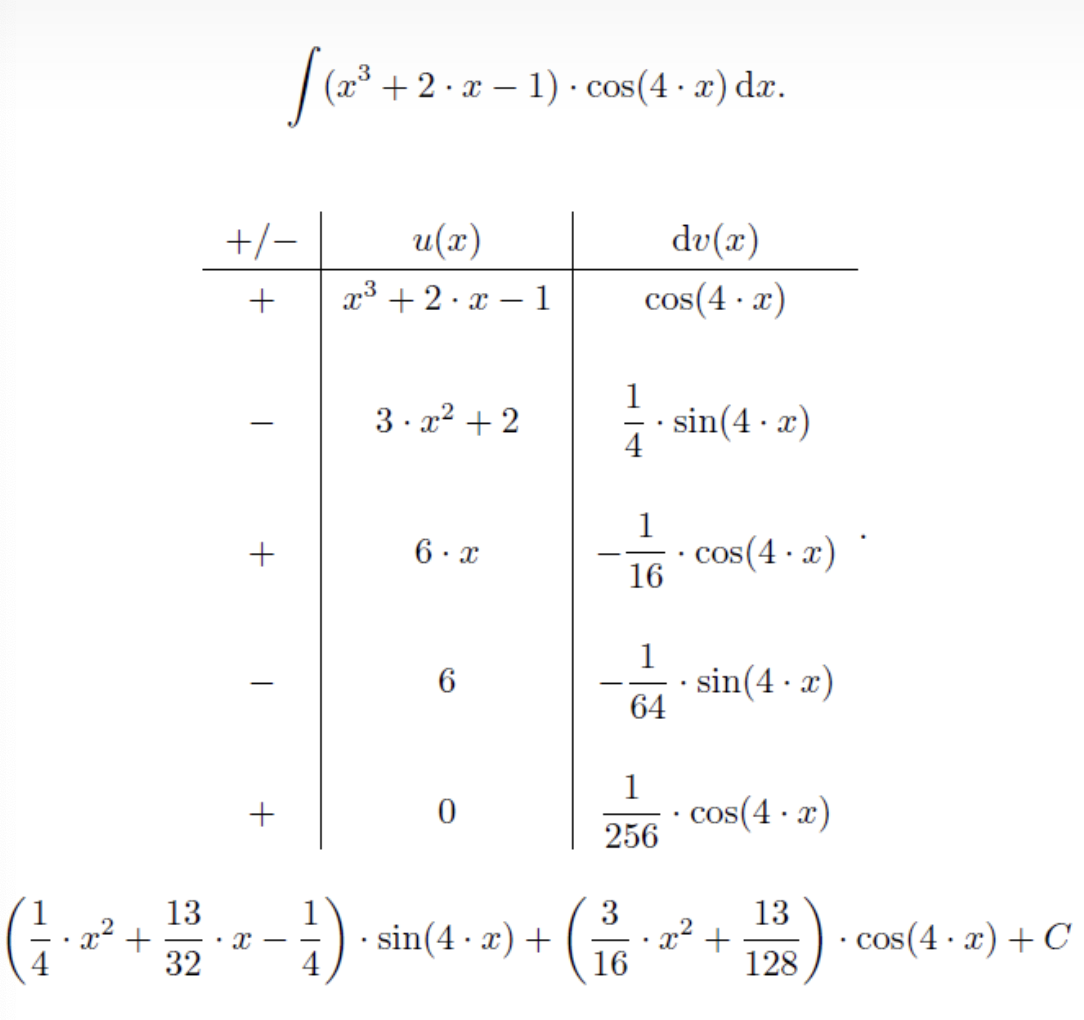
\includegraphics[width=0.6\textwidth]{figs/2022-04-12-10-37-38.png}
	\end{alertblock}
	反、对、幂、三、指的顺序
\end{frame}

\begin{frame}{}
			\begin{alertblock}{分部积分计算定积分$\int_{0}^{\pi}   x^2 (\pi-x)^2   \cos nx dx $}
				$\psi (x) = x^2 (\pi-x)^2$ ,则:\\
				$\displaystyle \begin{array}{lllllllll}
					\psi ' (x) &=  2x(2x - \pi )(x - \pi ) \\
					\psi '' (x) &=  2\pi ^2 -12\pi x+12x^2 \\
					\psi ''' (x) &=  24x -12 \pi \\
					\psi^{(4)} (x) &=  24  \\
				\end{array}$ \\ 
				$\nu^{(4)} (x) = \cos nx$ , 则:\\
				$\displaystyle \begin{array}{lllllllll}
					\nu ''' (x) &= \dfrac{1}{n} \sin nx \\
					\nu '' (x) &= -\dfrac{1}{n^2} \cos nx \\
					\nu ' (x) &= -\dfrac{1}{n^3} \sin nx \\
					\nu (x) &= \dfrac{1}{n^4} \cos nx \\
				\end{array}$ \\ 
			\end{alertblock}
\end{frame}	
		
\begin{frame}
			应用分部积分公式 \\
			$\displaystyle \begin{array}{lllllllll}
				\int\limits_{0}^{\pi}  \psi (x) \nu^{(4)} (x)  dx 
				&= [ \psi \nu''' - \psi' \nu'' + \psi'' \nu' -\psi''' \nu ]|_0 ^\pi +	\int\limits_{0}^{\pi}  \psi^{(4)} (x)  \nu (x)  dx  \\
				&=  [ \psi \nu''' - \psi' \nu'' + \psi'' \nu' -\psi''' \nu ]|_0 ^\pi 
			\end{array}$ \\ 
			* (1)式中:$\int_{0}^{\pi}  \psi^{(4)} (x)  \nu (x)  dx = \frac{24}{n^4} \int_{0}^{\pi}  \cos nx dx =0$ \\
			(2)式中的第1和第3项等于零($\sin nx |_0 ^\pi$) \\
			(3)式中第二项含 $2x(2x - \pi )(x - \pi )|_0 ^\pi$也为零, 因此有:
			\begin{equation*}
				\int\limits_{0}^{\pi}  \psi (x) \nu^{(4)} (x)  dx = [-\psi''' \nu ]|_0 ^\pi =  -\dfrac{12 \pi}{n^4}  [\cos n\pi +1 ]
			\end{equation*}
\end{frame}	

\begin{frame}
	\frametitle{第三类边界条件}
	求第三类边界条件的固有值问题\\
	$\begin{array}{lllllllll}
	III & \begin{cases}
			X'' (x)  + \lambda X =0   ~~,~~ 0<x<L\\
			X' (0) =0, X (L) =0
	\end{cases}\\	
	& \begin{cases}
		\lambda_n=\dfrac{(2n+1)^2 \pi ^2}{4l^2}\\
		X_n(x) = \cos \sqrt{\lambda} x
	\end{cases}\\	
	IV&\begin{cases}
		X'' (x)  + \lambda X =0   ~~,~~ 0<x<L\\
		X (0) =0, X' (L) =0
	\end{cases} \\	
	& \begin{cases}
		\lambda_n=\dfrac{(2n+1)^2 \pi ^2}{4l^2}\\
		X_n(x) = \sin \sqrt{\lambda} x
    \end{cases}\\	
	\end{array}$ \\ 
\end{frame}	

\begin{frame}
	\frametitle{}
	作业-1、求解热传导方程初边值问题\\
	$\begin{array}{lllllllll}
		&\begin{cases}
			u_{t} =a^2u_{xx} ~~,~~ 0<x<l, t>0\\
			u(0,t) =u(l,t)=0 \\
			u(x,0) =x (l-x)
		\end{cases}\\	
		&\begin{cases}
			u_{t} =a^2u_{xx} ~~,~~ 0<x<l, t>0\\
			u_x(0,t) =u_x(l,t)=0 \\
			u(x,0) =x(l-x/2)
		\end{cases} \\	
	\end{array}$ \\ 
	2、求第三类边界条件固有值问题,并求固有函数的正交性\\
	$\begin{array}{lllllllll}
		& \begin{cases}
			X'' (x)  + \lambda X =0   ~~,~~ 0<x<L\\
			X' (0) =0, X (L) =0
		\end{cases}\\	
		&\begin{cases}
			X'' (x)  + \lambda X =0   ~~,~~ 0<x<L\\
			X (0) =0, X' (L) =0
		\end{cases} \\	
	\end{array}$ 	
\end{frame}	

\begin{frame}
	\frametitle{}
	3. 什么是固有值?有何用处?
	\\
	4. 什么是固有函数?与固有值有何关系? 
	\\
	5. 分离变量法的数学思想是什么?
	\\
	6. 什么是叠加原理?与分离变量法有何关系
	\\
	7. 正交性是什么意思?有何用处?
	\\
	8. 较复杂的分部积分法怎么用?	
\end{frame}	


%%%%%%%%%%%%%%%%%%%%%%%%%%%%%%%%%%%%%%%%%%%%%
\section{3.拉普拉斯方程}
\subsection{方程的建立}
\begin{frame}
	\frametitle{方程的建立}
	\begin{exampleblock} {例1、建立拉普拉斯方程}
		对于位于原点的质量为M的质点,试建立其引力势函数
		u(x,y,z,t) 所满足的方程 .
	\end{exampleblock}
	%%\usetikzlibrary {3d} 
	\tikzset{math3d/.style={x={(-0.353cm,-0.353cm)},z={(0cm,1cm)},y={(1cm,0cm)}}}
	\opencutright 
	\def\windowpagestuff{\flushright 
	\begin{tikzpicture}
		\def\k{1.5}
		\draw [ ->] (0,0,0) --  (0,0,2.5)  node[below] {$z$};
		\draw [ ->]  (0,0,0) -- (\k, 0,0)   node[right] {$x$};
		\draw [ ->]  (0,0,0) -- (0,\k, 0)    node[right] {$y$};
		\fill[black!100] (0,0,0) node[right]{$M$} circle(0.8ex);
		\begin{scope}[canvas is zy plane at x=0] \draw (0,0) circle (1cm);
			\draw (-1,0) -- (1,0) (0,-1) -- (0,1);
		\end{scope};
		\begin{scope}[canvas is zx plane at y=0] \draw (0,0) circle (1cm);
			\draw (-1,0) -- (1,0) (0,-1) -- (0,1);
		\end{scope};
		\begin{scope}[canvas is xy plane at z=0] \draw (0,0) circle (1cm);
			\draw (-1,0) -- (1,0) (0,-1) -- (0,1);
		\end{scope};
	\end{tikzpicture}	}
	~~~\hspace*{\fill} \\	
	~~~\hspace*{\fill} \\	
	\begin{cutout} {0}{6cm}{0pt}{5}
		\alert{ 解:}	建立如图坐标系,\\
		在空间任一点(x,y,z)放置试验质点m\\
 		m感受的力为:\\
		{$ \overrightarrow{F} =-G\dfrac{Mm}{r^3} \overrightarrow {r} $ }  ~~,~~ $r=\sqrt{x^2+y^2+z^2}$\\ 
		M激发的引力场强为 \\
		{ $ \overrightarrow{A} =\dfrac{GM}{r^3} \overrightarrow{r} $ }\\
	\end{cutout}
\end{frame}	

\begin{frame}
	\frametitle{}
	取无穷远处场强为零,则引力势为\\
	$\displaystyle  u = -\int_{r}^{\infty} \overrightarrow{A}\cdot d \overrightarrow{r} =- \int_{r}^{\infty} \frac{GM}{r^2} dr =- \frac{GM}{r} $ \\
	即有: $\overrightarrow{A} =-\nabla u$ \\
	封闭球面S内的质量通量为 \\
	$\displaystyle \oint_{S} \overrightarrow{A} \cdot d \overrightarrow{S} = \frac{GM}{r^2} 4\pi r^2 =\int  4\pi G  \rho d\tau$  \\
	由高斯定理可知:\\
	$ \displaystyle \oint_{S} \overrightarrow{A} \cdot d \overrightarrow{S} =\int  \nabla \cdot \overrightarrow{A} d\tau $\\
	因此: 
	\begin{equation*}
		\nabla \cdot \overrightarrow{A} = 4\pi G \rho
	\end{equation*}
	由于 $\nabla \cdot \overrightarrow{A} = \nabla \cdot \left(-\nabla u\right)= -\nabla ^2 u$ \\
	得泊松方程:
	\begin{equation*}
		\nabla ^2 u= -4\pi G \rho
	\end{equation*}	
\end{frame}	

\begin{frame}
	\frametitle{}
	对于无源区域,得拉普拉斯方程
	\begin{equation*}
		\nabla ^2  u =0 
	\end{equation*}
	定义拉普拉斯算子:
	\begin{equation*}
		\triangle  = \nabla ^2 = \frac{\partial ^2}{\partial x^2} +\frac{\partial^2 }{\partial y^2} +\frac{\partial^2  }{\partial z^2}	
	\end{equation*}
	拉普拉斯方程为:
	\begin{equation*}
		\triangle   u =0 
	\end{equation*}
	\begin{block}{Remark}
		拉普拉斯方程和泊松方程是描述各种势场的基本方程。
	\end{block}
\end{frame}	


\subsection{方程的求解}
\begin{frame}
	\frametitle{方程的求解}
	\begin{exampleblock} {例2、求解矩形区域拉普拉斯方程}
		$\displaystyle \begin{cases}
			u_{xx} +u_{yy} =0 ,~~~~ (0<x<a, 0<y<b)\\
			u(x,0)= f_1 (x) ,  u(x,b)= f_2 (x) \\
			u(0,y)= g_1 (y) ,  u(a,y)= g_2 (y) 
		\end{cases}$ \\
	\end{exampleblock}	
	\alert{ 解:}	这是第一类边界条件,但不是零边界条件,可转化为 \\
	$\displaystyle (A) \begin{cases}
		u_{xx} +u_{yy} =0 ,~~~~ (0<x<a, 0<y<b)\\
		u(x,0)= 0,  u(x,b)= 0 \\
		u(0,y)= g_1 (y) ,  u(a,y)= g_2 (y) 
	\end{cases}$ \\
	$\displaystyle (B) \begin{cases}
		u_{xx} +u_{yy} =0 ,~~~~ (0<x<a, 0<y<b)\\
		u(x,0)= f_1 (x) ,  u(x,b)= f_2 (x) \\
		u(0,y)= 0,  u(a,y)= 0 
	\end{cases}$ \\
\end{frame}	

\begin{frame}
	当然,还可以进一步分解成四个边值问题!
	$\displaystyle  (I) \begin{cases}
		u_{xx} +u_{yy} =0 ,~~~~ (0<x<a, 0<y<b)\\
		u(x,0)= 0,  u(x,b)= 0 \\
		u(0,y)= g_1 (y) ,  u(a,y)= 0
	\end{cases}$ \\
	$\displaystyle (II)  \begin{cases}
		u_{xx} +u_{yy} =0 ,~~~~ (0<x<a, 0<y<b)\\
		u(x,0)= 0,  u(x,b)= 0 \\
		u(0,y)= 0,  u(a,y)= g_2 (y) 
	\end{cases}$ \\
	$\displaystyle  (III)  \begin{cases}
		u_{xx} +u_{yy} =0 ,~~~~ (0<x<a, 0<y<b)\\
		u(x,0)= f_1 (x) ,  u(x,b)= 0 \\
		u(0,y)= 0,  u(a,y)= 0 
	\end{cases}$ \\	
	$\displaystyle  (IV)  \begin{cases}
		u_{xx} +u_{yy} =0 ,~~~~ (0<x<a, 0<y<b)\\
		u(x,0)= 0,  u(x,b)= f_2 (x) \\
		u(0,y)= 0,  u(a,y)= 0 
	\end{cases}$ \\	
\end{frame}		

\begin{frame}
	\frametitle{}
	 以方程(I)为例求解\\
	$\displaystyle \begin{cases}
		u_{xx} +u_{yy} =0 ,~~~~ (0<x<1, 0<y<1)\\
		u(x,0)= 0,  u(x,1)= 0 \\
		u(0,y)= g_1 (y) =\sin \pi y,  u(1,y)= 0
	\end{cases}$ \\
	\alert{ 解:}	设有 	$ u(x,y)=X(x) Y(y)$ ,代回原方程,得
	\begin{equation*}
		X~^{''}(x)Y(y) +X(x)Y~^{''}=0
	\end{equation*}
	\begin{equation*}
		-\frac{X~^{''}}{X}=\frac{Y~^{''} }{Y} =-\lambda 
	\end{equation*}	
	得两个常微分方程:
\end{frame}	

\begin{frame}
	\frametitle{}	
	方程(1):\\
	$\displaystyle  \begin{cases}
		Y~^{''} +\lambda Y=0  ~~,~~ 0<y<1\\
		Y(0)=0 ~~,~~Y(1)=0 
	\end{cases}$ \\	
	方程(2):\\
	$\displaystyle  \begin{cases}
		X~^{'} -\lambda X=0  ~~,~~ 0<x<1 \\
		X(0)=\sin \pi y~~,~~X(1)=0 
	\end{cases}$ \\	\vspace{0.3em}
	方程(1)是一类条件零边界固有值问题,公式:\\
	固有值:$\displaystyle  \lambda~_n=\frac{n^2\pi~^2}{l~^2} =n^2\pi~^2$ \\ 
	固有函数: $\displaystyle  Y~_n= \sin \frac{n\pi~}{l} y = \sin n \pi y $ \\	
\end{frame}	

\begin{frame}
	\frametitle{}	
	解方程II : 
	代入$\lambda_n$, 得:
	$\displaystyle  X~^{''} - n^2\pi~^2~X=0 $ \\
	特征方程有两相异实根,通解为: \\ 
	\begin{equation*}
		X_n(x)=C_n exp(n\pi x )+ D_n exp(-n\pi x )
	\end{equation*}	
	结合(1)(2),方程(I)的基本解:\\ 
	$\displaystyle \begin{array}{llll}
		u_n(x,y) &=& [C_n exp(n\pi x )+ D_n exp(-n\pi x )] \sin (n \pi y)  \\ 
		&=& [a_n \cosh (n\pi x )+ b_n \sinh(n\pi x ) ]\sin (n \pi y)  \\ 
	\end{array}$ \\
	叠加解:
	\begin{equation*}
		u(x, y)   = \sum\limits_{n=1}^{\infty }  [a_n \cosh (n\pi x )+ b_n \sinh (n\pi x ) ] \sin (n \pi y)  
	\end{equation*}	
\end{frame}	

\begin{frame}
	\frametitle{}	
	代入定解条件:$ u(0,y)=0$, 得 \\
	$ \sum\limits_{n=1}^{\infty }  a_n  \sin (n \pi y) =0 $ ,=> $ a_n=0$ \\
	因此:\\
	$	u(x,y)    = \sum\limits_{n=1}^{\infty }  b_n \sinh (n\pi x )  \sin (n \pi y)  $ \\ 
	代入定解条件:$u(1,y) = \sin \pi y $, 得
	\begin{equation*}
		u(1,y)    = \sum\limits_{n=1}^{\infty }  b_n \sinh (n\pi )  \sin (n \pi y)  = \sin \pi y
	\end{equation*}
	正交性,得:$ b_1\sinh\pi =1,~~ b_n=0~,~ (n>1)$	\\ 
	原方程得解:
	\begin{equation*}
		u(x,y)    = \dfrac{\sinh \pi x}{\sinh \pi}  \sin ( \pi y) 
	\end{equation*}	
\end{frame}	

\begin{frame}
	\frametitle{}	
	同理,可以求出其他三个方程的解,最终进行线性叠加,得到矩形区域拉普拉斯方程的解:
	\begin{equation*}
		u(x,y)    = u_I (x,y)  +   u_{II}(x,y)  + u_{III}(x,y)  + u_{IV}(x,y)  
	\end{equation*}	
\end{frame}	

\begin{frame}
	\frametitle{}	
	\begin{block}	{注: 双曲函数:}		
		$\displaystyle \begin{cases}
			&\sinh(x) = -i \sin(ix) = \frac{e^x -e^{-x}}{2} \\
			&\cosh(x) = \cos(ix) = \frac{e^x +e^{-x}}{2} 
		\end{cases}$ 
	\end{block}
	\begin{center}
	    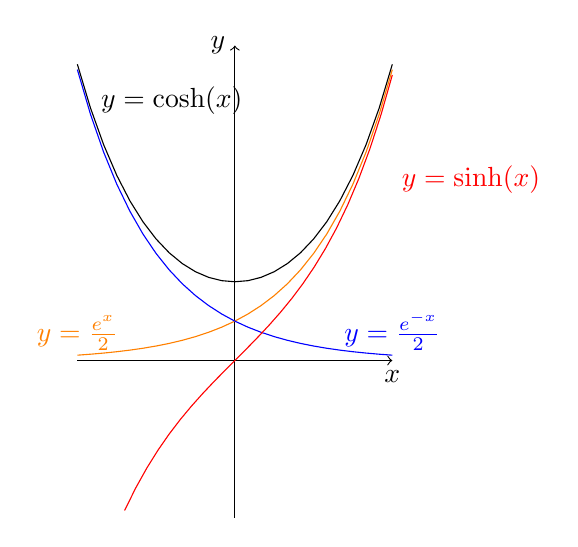
\begin{tikzpicture} 
    	\draw[->] (-2,0) -- (2,0) node[below] {$x$};
    	\draw[->] (0,-2) -- (0,4) node[left] {$y$};
    	\draw[orange, domain= -2:2]  plot (\x, {  exp(\x) * 0.5  } ) ;
    	\draw[orange]  (-2,0) node[above] {$y=\frac{e^ x}{2}$};
    	\draw[ blue, domain= -2:2]  plot (\x, {  exp(-\x) * 0.5  } );
    	\draw[blue]  (2,0) node[above] {$y=\frac{e^ {-x}}{2}$};
    	\draw[red, domain= -1.4:2]  plot (\x, {  exp(\x) * 0.5 -  exp(-\x) * 0.5 } ) ;
    	\draw[red]  (3,2) node[above] {$y=\sinh(x)$};
    	\draw[black, domain= -2:2]  plot (\x, {  exp(\x) * 0.5 +exp(-\x) * 0.5 } );
    	\draw[black]  (-0.8,3) node[above] {$y=\cosh(x)$};
	    \end{tikzpicture} 
	\end{center}
\end{frame}	

\subsection{区域边界条件}
\begin{frame}
	\frametitle{圆域拉普拉斯方程}	
	拉普拉斯算符在不同坐标系中的具体形式\\  \vspace{0.6 cm}	
	直角坐标~ $(x,y,z): $	{ 	$ \displaystyle  \nabla ^{2}  = \frac{\partial ^2}{\partial x^2} +\frac{\partial^2 }{\partial y^2} +\frac{\partial^2  }{\partial z^2}$}\\ 	
	球坐标~ $	(r,\theta, \varphi )$ :
	{ 	$ \displaystyle  \nabla ^{2} =\frac{1}{r^2} \frac{\partial }{\partial r} (r^2\frac{\partial }{\partial r} )+
		\frac{1}{r^2 \sin \theta  } \frac{\partial }{\partial \theta } (\sin \theta \frac{\partial }{\partial \theta } )
		+\frac{1}{r^2 \sin^2 \theta  } \frac{\partial^2}{\partial\varphi ^2}$ } \\ 	
	极坐标~ $	(r,\theta)$ :
	{ 	$ \displaystyle  \nabla ^{2} =\frac{\partial ^2 }{\partial r^2 } +\frac{1}{r } \frac{\partial }{\partial r } +
		\frac{1}{r^2 } \frac{\partial ^2 }{\partial \theta ^2 } $ }\\ 		
\end{frame}	
	
\begin{frame}	
	\begin{exampleblock} {例3、求圆域拉普拉斯方程}
	{ $  \displaystyle  \left \{ 
	\begin{array}{cc}
		\displaystyle {	\frac{\partial^2 u }{\partial r^2 } +\frac{1}{r } \frac{\partial u }{\partial r } +
			\frac{1}{r^2 } \frac{\partial ^2 u }{\partial \theta ^2
		} } =0, ~~ 0<r<r_0\\
		\\
		u(r_0,\theta )=f(\theta ) ,~~~~~~~~~~~~ 0<\theta <2\pi 
	\end{array}
	\right. $}  
	\end{exampleblock}	
	\alert{ 解:}	 
	方程可分离变量,令 $\displaystyle  u(r,\theta)=R(r) \Theta(\theta)$,代回原方程  \\ 
	{ $\displaystyle  R''\Theta +\dfrac{1}{r^2} R\Theta '' +\dfrac{1}{r}R'\Theta=0 $} \\ 
	{ $\displaystyle  \dfrac{r^2R''+rR'}{R}=-\dfrac{\Theta '' }{\Theta} =\lambda $} \\ 
	得两常微分方程:
\end{frame}	

\begin{frame}	
	I、 $\displaystyle 	\Theta '' + \lambda \theta =0 $  \\ 
	定解条件:$\displaystyle 	\Theta(\theta +2 \pi )=\Theta (\theta)  $  \\ 
	II、$\displaystyle  r^2 R'' +r R' -\lambda R =0 $  \\   \vspace{0.6 cm}	
	
	解方程I:  根据以前的分析,在 $\lambda > 0 $ 时,有通解\\ 
	{ $\displaystyle  \Theta(\theta)=A\cos \sqrt{\lambda } \theta+B\sin \sqrt{\lambda }\theta$}\\ 
	由定解条件:$\displaystyle 	\Theta(2 \pi )=\Theta (0)~,~~ 	\Theta' (2 \pi )=\Theta' (0)  $ 得方程: \\ 
	$ \left [
	\begin{array}{lll}
		\cos (\sqrt {\lambda} 2\pi )-1  & \sin (\sqrt {\lambda} 2\pi )\\
		-\sin (\sqrt {\lambda} 2\pi ) & \cos (\sqrt {\lambda} 2\pi )-1
	\end{array} \right] 
	\left [
	\begin{array}{lll}
		A\\
		B
	\end{array} \right] 
	=
	\left [
	\begin{array}{lll}
		0\\
		0
	\end{array} \right]
	$ \\
	系数行列式为零,得\\
	$(\cos (\sqrt {\lambda} 2\pi )-1 ) ^2 + \sin ^2 (\sqrt {\lambda} 2\pi ) =0$ \\ 
\end{frame}	

\begin{frame}
	$\cos (\sqrt {\lambda} 2\pi)=1$   \\ 	
	固有值:$\lambda _n =n^2 ~,~~ (n=0,1,2,...)$  \\ 
	固有函数:$\displaystyle  \Theta(\theta)=A_n\cos n \theta +B_n \sin n \theta $\\   \vspace{0.6cm}

	解方程II:
	{$\displaystyle  r^2 R'' +r R' -\lambda R =0 $  } \\ 
	把$\lambda_n =n^2 $代入, 得 \\ 
	{$\displaystyle  r^2 R'' +r R' -n^2R =0 $  } \\ 
	这是欧拉方程:令 $ r=exp(t) $ ,有 $t=\ln r$, 求导 \\ 
	$ \displaystyle \frac{dR}{dr} =\frac{dR}{dt} \frac{dt}{dr} =\frac{1}{r} \frac{dR}{dt} $ \\ 
	$ \displaystyle \frac{d^2R}{dr^2} =-\frac{1}{r^2}\frac{dR}{dt} + \frac{1}{r} \frac{d}{dr} (\frac{dR}{dt} )$ \\ 
	$ \displaystyle \frac{d^2R}{dr^2} =\frac{1}{r^2} (\frac{d^2R}{dt^2}-\frac{dR}{dt} )$ \\ 		
\end{frame}	

\begin{frame}	
	代回方程,得:\\ 
	$ \displaystyle   \dfrac{d^2R}{dt^2} -n^2 R =0 $ \\ 
	由特征方程有两相异实根,得通解:\\ 
	$ R=C_nexp(nt)+D_n exp(-nt) $\\
	把 $t=\ln r$ 代回,得\\
	$R=C_n r^n +D_nr^{-n}$ \\ 
	第二项发散,应删除,得\\
	$R= C_n r^n,  ~~ (n=0,1,2,......) $		\\
	基本解:\\ 
	$\begin{array}{llll}
		u_n(r,\theta) &=&  r^n(a_n \cos n\theta +b_n \sin n \theta )   \\ 
	\end{array}$ \\ 	
\end{frame}	

\begin{frame}	
	叠加解:\\ 
	$\begin{array}{llll}
		u(r, \theta) &=& \dfrac{1}{2} a_0 +\sum\limits_{n=1}^{\infty }r^n (a_n  \cos n\theta +b_n \sin n \theta ) 
	\end{array}$ \\ 
	代入定解条件:$ u(r_0,\theta)=f (\theta) =  \dfrac{1}{2} a_0 +\sum\limits_{n=1}^{\infty } (a_n\cos n\theta +b_n \sin n \theta ) r_0^n $\\ 
	系数公式:\\ 
	$  \displaystyle  a_n = \dfrac{1}{r_0 ^n \pi }  \int\limits_{0}^{2\pi} f(\theta) \cos n \theta d\theta $ \\ 
	$  \displaystyle  b_n = \dfrac{1}{r_0 ^n \pi }  \int\limits_{0}^{2\pi} f(\theta) \sin n \theta d\theta $  \\ 	
\end{frame}	

\begin{frame}	
	\begin{exampleblock} { 例4、求解如下边值问题}
	{ $  \displaystyle  \left \{ 
	\begin{array}{cc}
		\displaystyle {	\dfrac{\partial^2 u }{\partial r^2 } +\dfrac{1}{r } \dfrac{\partial u }{\partial r } +
		\dfrac{1}{r^2 } \dfrac{\partial ^2 u }{\partial \theta ^2
		} } =0, ~~ 0<r<r_0\\
		\\
		u(r_0,\theta )=A\cos(\theta),~~~~~~~~~ 0<\theta <2\pi 
	\end{array}
	\right. $}  
	\end{exampleblock}	
	\alert{ 解:}	 求系数:\\
	$  \displaystyle  a_1 = \dfrac{1}{r_0 ^1 \pi }  \int\limits_{0}^{2\pi} A\cos(\theta) \cos  \theta d\theta  $ \\ 	
	\hspace{0.8cm}$  \displaystyle  = \dfrac{A}{r_0  \pi }  \int\limits_{0}^{2\pi} \cos ^2 (\theta)  d\theta  = \frac{A}{r_0 \pi }  \int\limits_{0}^{2\pi} (1+\cos2\theta) d\theta$ = $\dfrac{2A}{r_0}$ \\ 
	$  \displaystyle  a_n = \dfrac{1}{r_0 ^n \pi }  \int\limits_{0}^{2\pi} A\cos(\theta) \cos n \theta d\theta =0~,~ (n\ne 1)$ \\ 
\end{frame}	

\begin{frame}	
	$  \displaystyle  b_n = \dfrac{1}{r_0 ^n \pi }  \int\limits_{0}^{2\pi} A\cos(\theta) \sin n \theta d\theta =0 $  \\ 
	叠加解:\\
	$\begin{array}{llll}
		u(r, \theta) &=& \dfrac{1}{2} a_0 +\sum\limits_{n=1}^{\infty } (a_n r^n\cos n\theta +b_n \sin n \theta )  \\
		&=& \dfrac{1}{2} a_0+ a_1 r\cos \theta \\
		&=&  \dfrac{A}{r_0} r \cos \theta 
	\end{array}$ \\ 
	\begin{block}{Remark}
		若将边界条件修改为: $A \cos 2\theta$ ,或 $A \sin 2\theta $ ,解会如何变化?
	\end{block}
\end{frame}	

\begin{frame}	
%	\frametitle{作业} 
	作业:
	1、求解固有值问题\\ 
	$\begin{array}{lllllllll}
		& \begin{cases}
			Y~^{''} +\lambda Y=0  ~~,~~ 0<y<2\pi \\
			Y(0) =Y(2\pi) , ~~ Y'(0) =Y'(2\pi)
		\end{cases}\\	
	\end{array}$ \\ 
	2、求解圆域边值问题\\
	$\displaystyle  \begin{array}{lllllllll}
	&\begin{cases}
		\dfrac{\partial^2 u }{\partial r^2 } +\dfrac{1}{r } \dfrac{\partial u }{\partial r } +
		\dfrac{1}{r^2 } \dfrac{\partial ^2 u }{\partial \theta ^2  } =0, ~~ 0<r<1\\
		u(1,\theta)= A\cos 2 \theta +B \cos 4 \theta \\	
	\end{cases} \\	
	\end{array}$ \\ 
	3、求解矩形域边值问题\\
	$\begin{array}{lllllllll}
		& \begin{cases}
			u_{xx} +u_{yy} =0 ,~~~~ (0<x, y<1)\\
			u(x,0)= u(0,y)=u(x,1)= 0 \\
			u(1,y)= \sin 2\pi y
		\end{cases}\\	
		&\begin{cases}
			u_{xx} +u_{yy} =0 ,~~~~ (0<x, y<1)\\
			u(1,y)= u(0,y)=u(x,0)= 0 \\
			u(x,1)= \sin n\pi x
		\end{cases} \\	
	\end{array}$ \\ 	
\end{frame}

\begin{frame}
	\frametitle{课外读物和思考}
	了解和学习三大偏微分方程的各种解法:\\
	《Partial Differential Equations》- 作者: Lawrence C. Evans \\
	《An Introduction to Partial Differential Equations》- 作者: M. Renardy R. C. Rogers
\end{frame}
%%%%%%%%%%%%%%%%%%%%%%%%%%%%%%			
     
%%%%%%%%%%%%%%%%%%%%%%%%%%%%%%%%%%%%%%%%%%%%%%%%%
\begin{frame}
		\frametitle{}
		\Background[1] 
	    \begin{center}
		{ {\Huge 第三章~~薛定谔方程 (I)\\(6学时)}}
	    \end{center}    
\end{frame}
%%%%%%%%%%%%%%%%%%%%%%%%%%%%%%%%%%%%%%%%%%%%%

\section{1.薛定谔方程基础}
\subsection{薛定谔方程}
\begin{frame}
	\frametitle{}  
	\begin{block}	{量子力学有关波函数的基本结论}
	\begin{itemize}
		\item 	波函数$\Psi$完全描述体系的状态,
		\item 	波函数的模方与粒子出现的概率成比例,$\omega \sim |\Psi|^2$
		\item 	波函数的演化服从薛定谔方程 : $\hat{E} \Psi = \hat{H}  \Psi $ 
	\end{itemize}
	薛定谔方程是量子力学基本方程,与牛顿力学的牛顿第二定理地位相当
	\end{block}	
\end{frame}

%%%%%%%%%%%%%%%%%%%%%%%%%%%%%%%%%%%%%%%%%%%%%
\begin{frame}
	\frametitle{方程的建立}
	\begin{alertblock} {可能思路}  
		\begin{itemize}
			\Item 	\textbf{1:}  最小作用量原理 $\int\limits_{t_1}^{t_2} \delta L d t =0 $\\ 
			\Item 	\textbf{2:}  波粒二象性\\ 
			~\\ 
			\Item 	\textbf{3:}  基本假设,不能从现有理论推导\\
            ~\\ 
            \begin{quote}
            "It is not possible to derive it from anything you know. It came out of the \alert{\faHeartbeat} of Schr$\ddot{o}$dinger"\\
            \rightline{$\cdots$ R. P. Feynman \hspace{3em}}   
            \end{quote}
		\end{itemize}
	\end{alertblock}
\end{frame}
\begin{frame}
	\frametitle{含时薛定谔方程}
	标准形式:    
	 \begin{equation*}
		i\hbar \frac{\partial }{\partial t} \Psi (\overrightarrow{r},t ) =\left [ -\frac{\hbar^2}{2\mu }\nabla ^2 + V(\overrightarrow{r},t ) \right ]\Psi (\overrightarrow{r}, t ) 
	\end{equation*}
	若取 $ \displaystyle  i\hbar \frac{\partial }{\partial t} ~~\to ~~ \hat{E} ~~, ~~  -\frac{\hbar^2}{2\mu }\nabla ^2 + V(\vec{r},t ) ~~\to ~~ \hat{H} $ \\
	算符形式:   \\ 
	\begin{equation*}
		\hat{E} ~ \Psi (\overrightarrow{r},t )  = \hat{H} ~ \Psi (\overrightarrow{r},t )  
	\end{equation*}
\end{frame}

\subsection{分离变量}

\begin{frame}
	\frametitle{分离变量}
	\begin{alertblock} {薛定谔方程$\hat{E} \Psi = \hat{H}  \Psi $ 为什么难求解?因为很难分离变量!}
		~~\\
		多粒子体系的波函数:
		\begin{equation*}
			\Psi (\vec{r_1},\vec{r_2},...,\vec{r_n},t )
		\end{equation*}		
		多粒子体系的哈密顿量:
		\begin{equation*}
			\hat{H} ~=\sum_{i=1}^{n} -\frac{\hbar^2}{2\mu }\nabla ^2 _i + \sum_{i=1}^{n} V(\vec{r_i},t) + \sum_{i,j=1, i\ne j}^{n}  U(\vec{r_i},\vec{r_j}) 
		\end{equation*}	
		有可能分离变量吗?条件呢?
	\end{alertblock}	
\end{frame}

\begin{frame}
\frametitle{分离变量(1)->固有值问题->定态薛定谔方程}
	若势函数$V(\vec{r},t ) $不显含时间$t$,时间变量可分离 \\ \vspace{0.3cm}
	方程: { $ \displaystyle i \hbar \frac{\partial }{\partial t} \Psi (\vec{r},t ) =\left [- \frac{\hbar^2}{2\mu }\nabla ^2 + V(\vec{r}) \right ]\Psi (\vec{r},t ) $}  \\  \vspace{0.3cm}
	\alert{解:}  设  $\Psi (\vec{r},t )  = \Psi (\vec{r} ) f(t) $ , 代回方程 \\ \vspace{0.6em}
	{ $ \displaystyle i\hbar \Psi (\vec{r})  \frac{\partial }{\partial t} f(t)=f(t) \left [ -\frac{\hbar^2}{2\mu }\nabla ^2 + V(\vec{r}) \right ]\Psi (\vec{r}) $}  \\ 	
	{ $ \displaystyle i\hbar \frac{1}{f(t)}  \frac{\partial }{\partial t} f(t)= \frac{1}{\Psi (\vec{r}) } \left [ -\frac{\hbar^2}{2\mu }\nabla ^2 + V(\vec{r}) \right ]\Psi (\vec{r}) =E $}  \\ 	
\end{frame}

\begin{frame}
	\frametitle{}
	得两个微分方程:\\  \vspace{0.3cm}
	I、演化问题(方程)  \[ \displaystyle  i\hbar \frac{1}{f(t)}  \frac{\partial }{\partial t} f(t)=E \]   
	解方程,得:$\displaystyle  f(t) =e^{-iEt/\hbar}$ \\  \vspace{0.6cm}
	II、固有值问题(定态薛定谔方程) \[\displaystyle   \left [ -\frac{\hbar^2}{2\mu }\nabla ^2 + V(\vec{r}) \right ]\Psi (\vec{r}) =E \Psi (\vec{r})  \]   
	算符形式:\[   \hat{H} \Psi (\vec{r}) =E \Psi (\vec{r})    \] 
	哈密顿量决定固有值问题(定态薛定谔方程)求解难度!	
\end{frame}

\begin{frame}
	\frametitle{分离变量(2)->单粒子定态薛定谔方程}
	多粒子体系的定态薛定谔方程:   
	\begin{equation*}
		\left [ \sum\limits_{i=1}^{n} \hat{H}_i + \sum_{i,j=1, i\ne j}^{n}  U(\vec{r_i},\vec{r_j}) \right ]	\Psi (\vec{r_1},\vec{r_2},...,\vec{r_n})=E 	\Psi (\vec{r_1},\vec{r_2},...,\vec{r_n})
	\end{equation*}		
	\alert{解:}  	对于无相互作用体系, 
	有$ U(\vec{r_i},\vec{r_j}) =0 $,\\
	 $ \hat{H}= \sum\limits_{i=1}^{n} (-\dfrac{\hbar^2}{2\mu }\nabla ^2 _i + V(\vec{r_i})) =\sum\limits_{i=1}^{n} \hat{H}_i \qquad (1)$\\   \vspace{0.3cm}
	方程可进一步分离变量!令 : \\
	 $\displaystyle \begin{cases}
	   	\Psi (\vec{r_1},\vec{r_2},...,\vec{r_n}) = \Psi (\vec{r_1}) \Psi (\vec{r_2})...\Psi (\vec{r_n}) \qquad (2) \\
		E= E_1+ E_2 + ... + E_n=\sum\limits_{i=1}^{n} \hat{E}_i \qquad (3)
	\end{cases}$ \\ \vspace{0.3em}
 	把(1)(2)(3)代回原方程
\end{frame}

\begin{frame}
	\frametitle{}
	获得如下方程
	\[ \sum\limits_{i=1}^{n} \hat{H}_i\Psi (\vec{r_1}) \Psi (\vec{r_2})...\Psi (\vec{r_n})= \sum\limits_{i=1}^{n} \hat{E}_i\Psi (\vec{r_1}) \Psi (\vec{r_2})...\Psi (\vec{r_n}) \]
	进一步简化,得单粒子定态薛定谔方程组\\
	$\displaystyle \begin{cases}
		\hat{H}_1\Psi (\vec{r_1})=E_1 \Psi (\vec{r_1})  \\  
		\hat{H}_2\Psi (\vec{r_2})=E_2 \Psi (\vec{r_2})  \\
		\dots\\
		\hat{H}_n\Psi (\vec{r_n})=E_n \Psi (\vec{r_n})  \\
	\end{cases}$ \\	
\end{frame}

\begin{frame}
	\frametitle{分离变量(3)->一维定态薛定谔方程} 
	单粒子定态薛定谔方程标准型
	\begin{equation*}
		\left [ -\dfrac{\hbar^2}{2\mu }\nabla ^2 + V(x,y,z) \right ]\Psi (x,y,z) =E \Psi (x,y,z)  
	\end{equation*}		
	\alert{解:} 若势函数 $ V(x,y,z)=V_1(x)+V_2(y)+V_3(z) $,则  $ \hat{H}=\hat{H}(x)+\hat{H}(y)+\hat{H}(z) $\\
	进一步分离变量:设  $$\Psi (x,y,z)  = \Psi_1 (x)\Psi_2 (y) \Psi_3 (z), \qquad  E= E_x+ E_y+E_z $$ \\
	代回, 得一维薛定谔方程(组)
	$\displaystyle \begin{cases}
		\hat{H}(x)\Psi_1 (x)=E_x \Psi_1 (x) \\
		\hat{H}(y)\Psi _2 (y)=E_y \Psi _2 (y)  \\
		\hat{H}(z)\Psi _3 (z)=E_z \Psi _3 (z) 
	\end{cases}$ \\	
\end{frame}

\begin{frame}
	\frametitle{}	
	如果势函数 $$ V(x,y,z)=V(r,\theta,\varphi) =V_1(r)+V_2(\theta)+V_3(\varphi) $$
	令  $$ \hat{H}=\hat{H}(r)+\hat{H}(\theta)+\hat{H}(\varphi) $$
	分离变量得一维薛定谔方程:\\
	$\displaystyle \begin{cases}
		\hat{H}(r)\Psi_1 (r)=E_r \Psi_1 (r) \\
		\hat{H}(\theta)\Psi _2 (\theta)=E_\theta \Psi _2 (\theta)  \\
		\hat{H}(\varphi)\Psi _3 (\varphi)=E_\varphi \Psi _3 (\varphi) 
	\end{cases}$ \\	
\end{frame}

%%%%%%%%%%%%%%%%%%%%%%%%%%%%%%%%%%%%%%%%%%%%%
\section{2.无限深势阱}

\begin{frame}
	\frametitle{}
	\begin{exampleblock} {例1、	一维无限深势阱I}
	一粒子处于如下一维无限深势阱,求解含时薛定谔方程\\
 	{ $ \displaystyle 
	V(x)=\left \{ 
	\begin{array}{cccc}
		0	~~ ~~ 0<x<a \\  
		+\infty ~~x<0, x>a\\
	\end{array}
	\right.
	$} \\
	\end{exampleblock} %2
	\alert{解:} 	势函数不显含时间t,含时薛定谔方程可分离变量,时间演化方程已求得(见前),现求定态薛定谔方程:\\
	{  $ \displaystyle 
	\left \{ 
	\begin{array}{cccc}
		\left [ -\dfrac{\hbar^2}{2\mu} \dfrac{\mathrm{d} ^2}{\mathrm{d} x^2} +0 \right ]\Psi(x)=E\Psi(x)  ~~ ~~ 0<x<a,~~~~~~~~ (1)  \\ 
		\\	
		\left [ -\dfrac{\hbar^2}{2\mu} \dfrac{\mathrm{d} ^2}{\mathrm{d} x^2} +\infty \right ]\Psi(x)=E\Psi(x)  ~~ ~~ x<0,~ x>a ~~~~~(2)  \\
	\end{array}
	\right.
	$} \\
\end{frame}

\begin{frame}
	\frametitle{}
	方程(2):解为  $\Psi(x) = 0$ \\ 
    方程(1):令 $ k^2= \dfrac{2\mu E}{\hbar ^2} $, 方程是如下边值问题:  \\ 
	{ $ \displaystyle 
		\begin{cases}
			\Psi''(x) + k^2	\Psi(x)=0  \\
			\Psi(0)=0~,~~ \Psi(a)=0 ~~~~~
		\end{cases}
		$} \\  \vspace{0.3cm}
    特征方程有两虚根,通解为:\\
     	\begin{equation*}
  			\Psi(x) = A\cos(kx) +B\sin(kx) 
    	\end{equation*}
    取$x=0, x=a$,  代入上式,由零边值条件得:\\
   	\hspace{2cm} $A=0, ~~~~ \sin ka =0$  \\  \vspace{0.3cm}
	有:$ka=n\pi  \to  k=\dfrac{n\pi}{a} = \sqrt{\dfrac{2\mu E}{\hbar ^2}}$    \\ 
\end{frame}

\begin{frame}
	\frametitle{}
	固有值(能级):{ $E_n = \dfrac{n^2\pi^2\hbar^2}{2\mu a^2} (n=1,2,3,...)$} \\
	能级间隔:  $\triangle E = E_{n+1}-E_n=\dfrac{\pi^2 \hbar^2}{2\mu a^2} (2n+1)$ \\ 
	固有函数: $ \Psi_n(x) = B_n\sin(\dfrac{n\pi}{a}x)  = \sqrt{\dfrac{2}{a}} \sin(\dfrac{n\pi}{a}x)$ \\ 
	\alert{归一化}: $ \int \limits_{0}^{a}  \Psi_n ^*(x)  \Psi_n(x)dx = \int \limits_{0}^{a}  |B_n| ^2 \sin^2(\dfrac{n\pi}{a}x) dx =1$  \\ 
	系数:$B_n=\sqrt{\dfrac{2}{a}}$ \\ 
	解函数: \\
	{  $ \displaystyle 
		\Psi_n(x,t)= \left \{ 
		\begin{array}{cccc}
			\sqrt{\dfrac{2}{a}} \sin(\dfrac{n\pi}{a}x) e^{-\dfrac{i}{\hbar} E_n t} ~~~~   0<x<a \\
			0 ~~~~~~~~~~~~~~~~~~~~~~~ x<0,x>a  
		\end{array}
		\right.
		$} \\	
\end{frame}

\begin{frame}
	\frametitle{}
  叠加解:
	  \[\Psi_(x,t)= A_n \psi_n(x,t)\]

  (1)给出定解条件,如何求$A_n$ \\ 
  (2)势阱有变化.如何解方程\\ \vspace*{0.6em}
	 {$ \displaystyle 
   V(x)=\left \{ 
   \begin{array}{cccc}
	   0+1	~~ ~~ 0<x<a \\  
	   +\infty ~~x<0, x>a\\
   \end{array}
   \right.
   ;$} \\ \vspace*{0.3em}
   {$ \displaystyle  V(x)=\left \{ 
	  \begin{array}{cccc}
		  0	~~ ~~ -a<x<a \\  
		  +\infty ~~x<-a, x>a\\
	  \end{array}
	  \right.
  ;$}\\ \vspace*{0.3em}
  {$ \displaystyle   V(x)=\left \{ 
	  \begin{array}{cccc}
		  0	~~ ~~ -\frac{a}{2}<x<\frac{a}{2} \\  
		  +\infty ~~x<-\frac{a}{2}, x>\frac{a}{2}\\
	  \end{array}
	  \right.
   $} \\
\end{frame}

\begin{frame}
	\frametitle{}
	%\usetikzlibrary {datavisualization.formats.functions} 
	\begin{center}
	\begin{tikzpicture}[baseline, scale=.6]
	\datavisualization [ scientific axes, 
		visualize as smooth line/.list={sin,cos,tan}, style sheet=strong colors,
		style sheet=vary dashing,
		sin={label in legend={text=$\Psi_1$}}, 
		cos={label in legend={text=$\Psi_2 $}}, 
		tan={label in legend={text=$\Psi_3 $}}, 
		data/format=function ]
		data [set=sin] {
			var x : interval [0:1];
			func y = sin(pi* \value x r ) * 1.414;
		}
		data [set=cos] {
			var x : interval [0:1];
			func y = sin(2*pi* \value x r ) * 1.414;
		}
		data [set=tan] {
			var x : interval [0:1];
			func y = sin(3*pi* \value x r ) * 1.414;
		};
	\end{tikzpicture} \\ \vspace{0.3cm}
	\end{center}
	\begin{center}
	\begin{tikzpicture}[baseline, scale=.6]
		\datavisualization [ scientific axes, 
		visualize as smooth line/.list={sin,cos,tan}, style sheet=strong colors,
		style sheet=vary dashing,
		sin={label in legend={text=$|\Psi_1|^2$}}, 
		cos={label in legend={text=$|\Psi_2|^2$}}, 
		tan={label in legend={text=$|\Psi_3|^2$}}, 
		data/format=function ]
		data [set=sin] {
			var x : interval [0:1];
			func y = sin(pi* \value x r ) *sin(pi* \value x r ) *2;
		}
		data [set=cos] {
			var x : interval [0:1];
			func y = sin(2*pi* \value x r ) *sin(2*pi* \value x r ) *2;
		}
		data [set=tan] {
			var x : interval [0:1];
			func y = sin(3*pi* \value x r ) * sin(3*pi* \value x r ) *2;
		};
	\end{tikzpicture}
	\end{center}
\end{frame}

\begin{frame}
	\frametitle{}
	\begin{exampleblock} {例2、无限深势阱II}
		设有一粒子处于如下一维无限深势阱中,求解薛定谔方程\\
		{ $ \displaystyle 
			V(x)=\left \{ 
			\begin{array}{cccc}
				0	~~ ~~ |x|<\dfrac{a}{2} \\  
				+\infty ~~|x|>\dfrac{a}{2}\\
			\end{array}
			\right.
		$} \\
	\end{exampleblock}
	\alert{解:} 	势函数与上例存在平移关系, 令$x' =x+a/2$\\
	有:  $  \sin(\dfrac{n\pi}{a}x') =\sin(\dfrac{n\pi}{a} (x+a/2)) $ \\
	\hspace{2cm}$=\sin \dfrac{n\pi}{a} x \cos \dfrac{n\pi}{2} + \cos \dfrac{n\pi}{a} x \sin \dfrac{n\pi}{2}  $ \\ 
	n为偶数: $E_{2m} = \dfrac{2m^2\pi^2\hbar^2}{\mu a^2} $\\
	\hspace{2cm}$ \Psi_{2m}(x)= B_{2m} \sin(\dfrac{2m\pi}{a}x) $,   \\
\end{frame}

\begin{frame}
	\frametitle{}
	n为奇数:  $E_{2m+1} = \frac{(2m+1)^2\pi^2\hbar^2}{2\mu a^2} $ \\
	\hspace{2cm}$ \Psi_{2m+1}(x)= B_{2m+1} \cos(\dfrac{(2m+1)\pi}{a}x) $,  \\
	归一化,求系数 ... \\	 \vspace{0.6cm}	
	\textbf{如果把势阱宽改为2a}, 直接求解, 可得: \\
	固有值(能级):{ $E_n = \dfrac{n^2\pi^2\hbar^2}{8\mu a^2} (n=1,2,3,...)$} \\
	固有函数: $ \Psi_n(x)= \sqrt{\dfrac{2}{a}} \sin(\dfrac{n\pi}{a}(x+a)) $ \\  \vspace{0.6cm}	
	比较两种解之间的关系!	明确势阱平移与伸缩后解的写法。
\end{frame}

\begin{frame}
	\frametitle{}
	\begin{exampleblock} {例3、无限深势阱III}
	求解一维无限深势阱的非定常问题 \\
		{ $ \displaystyle 
			\begin{cases}
				i\hbar \dfrac{\partial }{\partial t} \Psi = -\dfrac{\hbar^2}{2\mu } \dfrac{\partial ^2 \Psi }{\partial ^2  x ^2 } , ~~ (0<x<L, t>0) \\
				\Psi (0,t) =0, ~~ \Psi (L,t) =0 \\
				\Psi (x,0) =f(x)  \\
			\end{cases}
		$} \\
	\end{exampleblock}
	\alert{解:} 	令$\Psi (x,t) =\Psi (x) T(t) $ ,  代回方程, 得:\\
	{ $ \displaystyle 
	\begin{cases}
		\Psi''(x) + k^2	\Psi(x)=0  \\
		\Psi(0)=0~,~~ \Psi(L)=0 ~~~~~
	\end{cases}
	$} \\
	固有值: $E_n = \dfrac{n^2\pi^2\hbar^2}{2\mu L^2} (n=1,2,3,...)$\\
	固有函数: $ \Psi_n(x) = \sin(\dfrac{n\pi}{L}x) $ 	 \\ 
\end{frame}

\begin{frame}
	\frametitle{}
	时间函数: $T_n(t)  = \exp(-i E_n t /\hbar) $ \\
	级数解为:  $ \Psi(x,t)  = \sum\limits_{n=1}^{\infty}  B_n \exp(-i E_n t /\hbar)  \sin(\dfrac{n\pi}{L}x)  $ \\
	取 t=0, 代入初值条件, 得:  $ f(x)= \sum\limits_{n=1}^{\infty}  B_n \sin(\dfrac{n\pi}{L}x)  $ \\
	得系数:  $ B_n= \dfrac{2}{L} \int\limits_{0} ^{L}  \sin(\dfrac{n\pi}{L}x) dx, ~~ (n=1,2,3,...) $ \\
\end{frame}

\begin{frame}
	\frametitle{作业}
	1、求定态薛定谔方程\\ 
	$\begin{array}{lllllllll}
		& \begin{cases}
			\Psi'' (x) +\dfrac{2\mu E}{\hbar ^2} \Psi(x) =0,~~ |x|<a/2 \\
			\Psi(-a/2) =\Psi(a/2) =0\\
		\end{cases}\\	
	\end{array}$ \\ 
	2、求解非定常问题\\
	$\begin{array}{lllllllll}
		& \begin{cases}
			i\hbar \dfrac{\partial }{\partial t} \Psi = -\dfrac{\hbar^2}{2\mu } \dfrac{\partial ^2 \Psi }{\partial ^2  x ^2 } , ~~ (0<x<L, t>0) \\
			\Psi (0,t) =0, ~~ \Psi (L,t) =0 \\
			\Psi (x,0) =f(x)  \\
		\end{cases}\\
	\end{array}$ \\ 
	3、求三维无限势阱问题\\
	$ ~~~~	V(x,y,z)=\left \{ 
	\begin{array}{cccc}
		0	~~ ,~~ 0<x,y,z<a \\  
		+\infty ,~~others\
	\end{array}
	\right. $ 	
	4. 求自由粒子的一维薛定谔方程\\
\end{frame}

%%%%%%%%%%%%%%%%%%%%%%%%%%%%%%%%%%%%%%%%%%%%%
\section{3.量子谐振子与厄密方程}

\subsection{相互作用势}

\begin{frame}
	\frametitle{相互作用势}
	\begin{exampleblock} {例1、相互作用势的二阶近似}
		半经验Lennard-Jones势(如图所示)\\ \vspace{0.6em }
	   \centerline{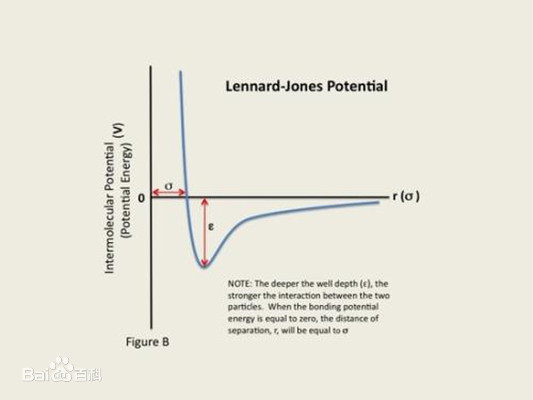
\includegraphics[width=0.45\textwidth]{LJpotential}}  
		实际的相互作用势V(x) 较L-J势更复杂,试求其在平衡位置附近的二阶近似	
	\end{exampleblock}
\end{frame}

\begin{frame}
	\frametitle{}
	\alert{解:} 	不管多复杂,在平衡位置 ($x=a$)附近可泰勒展开
	\begin{equation*}
		V(x)=V(a) +\frac{1}{1!} \frac{\partial V}{\partial x} |_{x=a} (x-a) +\frac{1}{2!} \frac{\partial ^2 V}{\partial x ^2} |_{x=a} (x-a) ^2 + ... 
	\end{equation*}
	一阶导应为零,二阶近似可写为 \\
	$\displaystyle  \begin{array}{lllllllll}
		V(x) &\approx V(a)+\dfrac{1}{2!} \dfrac{\partial ^2 V}{\partial x ^2} |_{x=a} (x-a) ^2   \\
		& =V_0+\dfrac{1}{2} k (x-a) ^2 
	\end{array}$\\
	取坐标原点为($a, V_0 $), 得:\\
	\begin{equation*}
		V(x)=\dfrac{1}{2} k x^2 
	\end{equation*}	
\end{frame}

\begin{frame}
	\frametitle{}
	\begin{block}{弹性势}
		~~\\
		弹簧力正是势函数V(x) 在平衡位置附近的二阶近似\\
		\begin{equation*}
			F=-\frac{ \partial V}{\partial x}=-kx 
		\end{equation*}	
		 把势函数V(x) 改写成弹性势能:\\
		\begin{equation*}
			U(x)=\dfrac{1}{2} \mu \omega ^2 x^2 
		\end{equation*}
	\end{block}	
\end{frame}	

\subsection{量子谐振子方程}

\begin{frame}
	\frametitle{量子谐振子方程}
	\begin{exampleblock} {例2、求解谐振子薛定谔方程}
	\begin{equation*}
		i\hbar \frac{\partial }{\partial t} \Psi (x,t ) =[ -\frac{\hbar^2}{2\mu } \frac{d ^2}{x^2} + \frac{1}{2} \mu \omega ^2 x^2   ] \Psi (x, t ) 
	\end{equation*}
	\end{exampleblock}
	\alert{解:} 	令$\Psi (x,t) =\Psi(x) T(t) $ ,  代回方程\\
	时间和位置分离变量:\\
	时间函数: $T(t)  = \exp(-i E t /\hbar) $ \\
	位置函数满足定态薛定谔方程\\
	\begin{equation*}
		\left [ -\frac{\hbar^2}{2\mu} \frac{\mathrm{d} ^2}{\mathrm{d} x^2} +\frac{1}{2}\mu \omega^2 x^2  \right ]\Psi(x)=E\Psi(x) 
	\end{equation*}	
\end{frame}

\begin{frame}
	\frametitle{}
	整理:\\
	\begin{equation*}
		\frac{1}{\dfrac{\mu\omega}{\hbar}} \frac{\mathrm{d} ^2\Psi}{\mathrm{d} x^2} +	\left ( \frac{2E}{\omega \hbar} -\frac{\mu \omega}{\hbar} x^2 \right )\Psi=0
	\end{equation*}
	令:~~$ \xi =\alpha x$,做自变量伸缩变换 \\
	\begin{equation*}
		\frac{\mathrm{d} \Psi}{\mathrm{d} x} =\frac{\mathrm{d} \Psi}{\mathrm{d} \xi} \frac{\mathrm{d} \xi}{\mathrm{d} x}  = \alpha \frac{\mathrm{d} \Psi}{\mathrm{d} \xi}
	\end{equation*}
	\begin{equation*}
		\frac{\mathrm{d} \Psi ^2 }{\mathrm{d} x ^2} =\frac{\mathrm{d}}{\mathrm{d} x}  ( \alpha \frac{\mathrm{d} \Psi}{\mathrm{d} \xi} ) = \alpha ^2 \frac{\mathrm{d} ^2 \Psi}{\mathrm{d} \xi ^2} 
	\end{equation*}
	代回方程, 得\\
	\begin{equation*}
		\left[ \frac{\hbar ^2 \alpha ^2 }{2\mu} \frac{\mathrm{d}}{\mathrm{d} \xi ^2}  + (E- \frac{\mu \omega ^2 \xi ^2}{2 \alpha ^2}  ) \right] \Psi(\xi) =0
	\end{equation*}	
\end{frame}

\begin{frame}
	\frametitle{}
	同除二阶导数项系数, 得\\
	\begin{equation*}
		\left[ \frac{\mathrm{d}}{\mathrm{d} \xi ^2}  + \frac{2\mu}{\hbar ^2 \alpha ^2 } (E- \frac{\mu \omega ^2 \xi ^2}{2 \alpha ^2}  ) \right] \Psi(\xi) =0
	\end{equation*}
	令 $\dfrac{\mu ^2 \omega ^2 }{\hbar ^2 \alpha ^ 4}=1 $,得伸缩系数:\\
	\begin{equation*}
		\alpha ^2= \frac{\mu\omega}{\hbar}
	\end{equation*}
	引入特征值\\
	\begin{equation*}
		\lambda = \frac{2E}{\omega \hbar}
	\end{equation*}
	得二阶常微分方程\\
	\begin{equation*}
		\left[ \frac{\mathrm{d} ^2\Psi}{\mathrm{d} \xi^2} + \left( \lambda - \xi^2 \right) \right] \Psi=0
	\end{equation*}
\end{frame}

\begin{frame}
	\frametitle{}
	考虑渐近行为, 当 $ |x| \to \infty,  \xi \to \infty$,有 $ \xi ^2  \gg  \lambda $,方程可近似为 \\
	\begin{equation*}
		\left(\frac{\mathrm{d} ^2}{\mathrm{d} \xi^2} - \xi^2 \right) \Psi=0
	\end{equation*}
	方程并无表达式解,但通过检验平方指数函数的导数\\
	\begin{equation*}
		\frac{d^2 }{d \xi ^2} \exp(\frac{\xi ^2}{2}) =(\xi ^2 +1)  \exp(\frac{\xi ^2}{2}) 
	\end{equation*}    
	\begin{equation*}
		\frac{d^2 }{d \xi ^2} \exp( - \frac{\xi ^2}{2}) =(\xi ^2 -1)  \exp( - \frac{\xi ^2}{2}) 
	\end{equation*}     	
\end{frame}

\begin{frame}
	\frametitle{}
	当 $ \xi \to \infty$, 这两导数可近似为:\\
	\begin{equation*}
		(\xi ^2 )  \exp( \frac{\xi ^2}{2}) ~~, ~~ (\xi ^2 )  \exp( - \frac{\xi ^2}{2}) 
	\end{equation*}     
	因此,极限状态解应与如下函数相关联
	\begin{equation*}
		C_1  \exp( \frac{\xi ^2}{2}) + C_2   \exp( - \frac{\xi ^2}{2})  
	\end{equation*}     
	考虑到波函数的有界性,应删除发散项(第一项),得极限状态波函数的简洁形式
	\begin{equation*}
		\Psi_\infty (\xi)  \sim C_2 \exp( - \frac{\xi ^2}{2})  
	\end{equation*}   
\end{frame}

\begin{frame}
	\frametitle{}
	现考虑非极限状态,解函数可写成: 
	\begin{equation*}
		\Psi(\xi) = H(\xi) e^{-\xi^2/2 }  
	\end{equation*}   
	解函数的确定等价于多项式函数 H 的确定。\\
	对上式求导:\\
	\begin{equation*}
		\Psi'(\xi) = H'(\xi) e^{-\xi^2/2 } -  H(\xi) \xi e^{-\xi^2/2 } 
	\end{equation*}  
	\begin{equation*}
		\Psi''(\xi) = \left[  \left( \xi^2 -1 \right) H -2\xi H' +H''  \right] e^{-\xi^2/2}
	\end{equation*}  
	代回原方程  $ \displaystyle \dfrac{\mathrm{d} ^2\Psi}{\mathrm{d} \xi^2} + \left( \lambda - \xi^2 \right) \Psi=0 $  \\ 
\end{frame}

\begin{frame}
	\frametitle{}
	得关于多项式$H(\xi)$的方程: \\  
	\begin{equation*}
		H'' -2 \xi H' +(\lambda -1) H=0 
	\end{equation*}  
	取$\lambda -1= 2n $,方程转化为n阶厄密方程
	\begin{equation*}
		H'' -2 \xi H' +2n H=0 
	\end{equation*}  
	由
	\begin{equation*}
		\lambda = 2n +1 = \frac{2E}{\hbar  \omega}  
	\end{equation*}  
	解出能量固有值(能级)
	\begin{equation*}
		E_n=\left(n+\frac{1}{2}\right) \hbar \omega, ~~~  ( n=0,1,2, ...)  
	\end{equation*}  
	固有函数由n阶厄密方程给出......
\end{frame}

%%%%%%%%%%%%%%%%%%%%%%%%%%%%%%%%%%
\subsection{厄密方程}

\begin{frame}
	\frametitle{厄密方程}
	\begin{exampleblock} {例3、求解n阶厄密方程}
		\begin{equation*}
			H'' -2 \xi H' +2n H=0 
		\end{equation*}  
	\end{exampleblock}
	\alert{解:} 	幂级数方法求解,令:
	\begin{equation*}
		H=\sum_{k=0}^{\infty} c_k \xi ^k
	\end{equation*}     
	求一阶导和二阶导,代回厄密方程,可得系数递推式:
	\begin{equation*}
		c_{k+2} = \frac{ 2(k-n)}{(k+2)(k+1) } c_k, ~~  \left( k=0,1,2,3, ...  \right)
	\end{equation*}   
\end{frame}

\begin{frame}
	\frametitle{}
	分偶数阶和奇数阶写
	\begin{equation*}
		c_{2m} = (-1) ^m \frac{2^mn(n-2)(n-4) ... (n-2m+2)  } {(2m)!} c_0
	\end{equation*}   
	显然有 $ c_{2m} =0~, ~~(2m>n)$
	\begin{equation*}
		c_{k} = (-1) ^m \frac{2^mn !! } {k!} c_0, ~~~(2m=k)
	\end{equation*}   
	\begin{equation*}
		c_{2m+1} = (-1) ^m \frac{2^m (n-1) (n-3)(n-5)...(n-2m+1)  } {(2m+1)!} c_1
	\end{equation*}   
	显然有 $ c_{2m+1} =0~, ~~(2m+1>n)$
	\begin{equation*}
		c_{k} = (-1) ^m \frac{2^m n!! }{k!} c_1, ~~~ (2m+1=k)
	\end{equation*}  
\end{frame}

\begin{frame}
	\frametitle{}
	所有系数求得,幂级数得解\\
	$\displaystyle \begin{cases}
		y_1(\xi)  = [1- \dfrac{2n}{2!} \xi^2+ \dfrac{2^2n(n-2)}{4!} \xi^4 -...  ] \\
		\\
		y_2(\xi)  = [\xi- \dfrac{2(n-1)}{3!} \xi^3+ \dfrac{2^2(n-1)(n-3) }{5!}\xi^5 -...  ]
	\end{cases}$ \\
	n阶厄密方程的解:
	\begin{equation*}
		H(\xi) =c_0y_1(\xi)+c_1 y_2(\xi).
	\end{equation*}   
 	 量子谐振子方程的解:
	\begin{equation*}
		\Psi(\xi) = [c_0y_1(\xi)+c_1 y_2(\xi) ]e^{-\xi^2/2 }  
  	\end{equation*}   
  	根据波函数的有界性性质, H应取多项式 (不能为无穷级数)。当n为偶数时 , $c_1=0$ , 当n为奇数时 , $c_0=0$ 。 待定系数由定解条件给出...
\end{frame}

\begin{frame}
	\frametitle{}
		为了更好地描述,将系数递推式降幂排列,现令最高次项系数为:
	\begin{equation*}
		c_n =2^n
	\end{equation*}  
	系数递推式可写为:
	\begin{equation*}
		c_{k-2} = -\frac{k(k-1) } { 2(n-k+2)}  c_k
	\end{equation*} 
	\begin{equation*}
		c_{n-2} = -\frac{n(n-1) } { 2\times2}  c_n
	\end{equation*} 
	\begin{equation*}
		c_{n-4} = (-1)^2 \frac{n(n-1)(n-2) (n-3) } { 2\times2\times 4}  2^n
	\end{equation*} 
		\begin{equation*}
		c_{n-2m} = (-1)^m \frac{n! } { 2^m (2m) !! (n-2m)!}  2^n =(-1)^m \frac{n! } {  m ! (n-2m)!}  2^{n-2m} 
	\end{equation*} 
\end{frame}

\begin{frame}
	\frametitle{}
	厄密方程的解为厄米多项式:
	\begin{equation*}
		H_n(\xi) =\sum_{m=0}^{M}  (-1)^m \frac{n! } {  m ! (n-2m)!}  2^{n-2m} \xi^{n-2m} ,  ~~~ M=[n/2]
	\end{equation*}   
	量子谐振子的解为
	\begin{equation*}
		\Psi_n(\xi) = N_n \exp(-\frac{\xi ^2}{2}) H_n(\xi) 
	\end{equation*}   
	归一化解:(...)
	\begin{equation*}
		\Psi_n(x) = \left( \frac{\alpha}{\sqrt{\pi} 2^n n!}  \right) ^{1/2}  \exp(-\frac{ \alpha^2 x^2}{2}) H_n( \alpha x) 
	\end{equation*}  
	定态波函数为
	\begin{equation*}
		\Psi_n(x,t) = \left( \frac{\alpha}{\sqrt{\pi} 2^n n!}  \right) ^{1/2}  \exp(-\frac{ \alpha^2 x^2}{2} -\frac{i}{\hbar} E_n t ) H_n( \alpha x) 
	\end{equation*}  	
\end{frame}

\begin{frame}
	\frametitle{作业:}
	1、计算积分\\ 
	$\begin{array}{lllllllll}
		 &\int\limits_{0}^{+\infty} e^{-x^2 /2} dx
	\end{array}$ \\ \vspace{0.6em}
	2、 根据厄米多项式表达式,写出前五个厄米多项式,并分析$H'_n (x)$ 与$H_{n-1} (x)$  之间的联系\\ \vspace{0.6em}
	3、 求解厄米方程\\ \vspace{0.6em}
	$\begin{array}{lllllllll}
		& \dfrac{d^2 H}{d x^2} -2x \dfrac{d y}{d x} +4n H =0 		
	\end{array}$ \\ \vspace{0.6em}
	4、  列出厄米方程的几种形式,说明厄米方程的特点
\end{frame}

%%%%%%%%%%%%%%%%%%%%%%%%%%%%%%%%%%%%%%%%%%%%%
\section{4.厄密多项式及性质}

\subsection{生成函数}

\begin{frame}
	\frametitle{ 生成函数 }
	\begin{exampleblock} { 例1、求厄密多项式的生成函数 }
		找一个函数,它的展开系数刚好就是Hermite 多项式
		 \begin{equation*}
			w(x,t)=e^{2xt-t^2}
		\end{equation*}
		试证明,上述二元函数就是Hermite多项式的一个母函数
	\end{exampleblock}
	\alert {解:}	把函数做关于变量t的Taylor 展开:
	\begin{equation*}
		w(x,t) =\sum_{n=0}^{\infty} \frac{1}{n!}  c_n(x) t^n
	\end{equation*}
	需证明:
	\begin{equation*}
		\left[  \frac{d^2}{dx^2} -2x\frac{d}{dx} +2n  \right] c_n(x)=0
	\end{equation*}
\end{frame}

\begin{frame}
	\frametitle{  }
	\textbf{证明:}	1)、由 $  \dfrac{\partial w}{\partial x} =2t e^{2xt-t^2} =2t ~w(x,t) $, 得 \\ 
	$ \sum\limits_{n=0}^{\infty} \dfrac{1}{n!}  c~'_n(x) t^n  = 2t  \sum\limits_{n=0}^{\infty} \dfrac{1}{n!}  c_n(x) t^n $ \\
	\hspace{2.3cm}	$=  \sum\limits_{n=0}^{\infty} \dfrac{1}{n!}  2c_{n}(x) t^{n+1} $\\
	\hspace{2.3cm}	$=  \sum\limits_{n=1}^{\infty} \dfrac{1}{n!}  2nc_{n-1}(x) t^{n}   $ \\
	比较系数,有:\\
	\hspace{2.1cm}	{ $c~'_n(x)=2nc_{n-1}(x)$} \\  \vspace{0.3cm}
	\hspace{2.1cm}	$c~''_n(x)=2nc~'_{n-1}(x)=4n(n-1)c_{n-2}(x)$ \\  	
\end{frame}

\begin{frame}
	\frametitle{  }
	2)由 $  \dfrac{\partial w}{\partial t} =2(x-t) e^{2xt-t^2} =2(x-t) ~w(x,t) $, 得 \\ 
	\hspace{2.1cm}		$  \dfrac{\partial w}{\partial t} +2(t-x) ~w(x,t) =0$ \\ 
	把展开式代入上式\\ 
	{$  \sum\limits_{n=1}^{\infty} \dfrac{1}{n!}n c_n(x) t^{n-1} +\sum\limits_{n=0}^{\infty} \dfrac{1}{n!}2(t-x) c_n(x)t^n=0$ } \\ \vspace{0.3cm}
	{$ \sum\limits_{n=1}^{\infty} \dfrac{1}{n!}n c_n(x) t^{n-1} +\sum\limits_{n=0}^{\infty} \dfrac{-2x}{n!} c_n(x)t^n +\sum\limits_{n=0}^{\infty}\dfrac{2}{n!} c_n(x)t^{n+1}=0$ } \\ \vspace{0.3cm}
	{$ \sum\limits_{n=0}^{\infty} \dfrac{1}{n!} c_{n+1}(x) t^{n} +\sum\limits_{n=0}^{\infty} \dfrac{-2x}{n!} c_n(x)t^n +\sum\limits_{n=1}^{\infty}\dfrac{2n}{n!} c_{n-1}(x)t^n=0$ } 
\end{frame}

\begin{frame}
	\frametitle{  }
	比较系数,有:\\
	\hspace{2.1cm}	{  $ c_{n+1}(x) -2xc_n(x) +2nc_{n-1} (x) =0 $} \\ \vspace{0.3cm}
	\hspace{2.1cm}	{  $ c_{n}(x) -2xc_{n-1}(x) +2(n-1)c_{n-2} (x) =0 $} \\ 
	3) 把(1)中得到的结论 \\
	\hspace{2.1cm}	{ $c~'_n(x)=2nc_{n-1}(x)$} \\  \vspace{0.3cm}
	\hspace{2.1cm}	$c~''_n(x)=4n(n-1)c_{n-2}(x)$ \\  
	代入(2)中得到的结论,得:\\
	\hspace{2.1cm} $  c_{n}(x) - \dfrac{x}{n}c~'_{n}(x) +\dfrac{1}{2n}c~''_{n} (x) =0 $ \\
	整理为:
	\begin{equation*}
 	    \left[  \dfrac{d^2}{dx^2} -2x\frac{d}{dx} +2n  \right] c_n(x)=0 
	\end{equation*}
 	\textcolor{red}{证毕!}\\
	即有: $c_n(x)=H_n(x)  $ 
\end{frame}

\subsection{性质}
\begin{frame}
	\frametitle{递推公式 }
	{  既然: $c_n(x)=H_n(x) $}  \\ \vspace{0.3cm}
	\hspace{1cm} 	{  $c~'_n(x)=2nc_{n-1}(x)    $ }   \\ 
	{  $ ~\to~~  H~'_n(x)=2nH_{n-1}(x)    $}   \\ \vspace{0.3cm}
	\hspace{1cm} 	{  $ c_{n}(x) -2xc_{n-1}(x) +2(n-1)c_{n-2} (x) =0  $ }   \\ 
	{  $~\to~~   H_{n}(x) -2xH_{n-1}(x) +2(n-1)H_{n-2} (x) =0  $ } \\ \vspace{0.3cm}
	有: $H_0(x)=1,  H_1(x)=2x, $	
\end{frame}

\begin{frame}
	\frametitle{ 微分形式 }
	$ \displaystyle w(x,t) =\sum_{n=0}^{\infty} \frac{1}{n!}  c_n(x) t^n $, ~~~~
	{ $ \displaystyle w(x,t) =\sum_{n=0}^{\infty} \frac{1}{n!}  H_n(x) t^n  $} \\
	由Taylor展式,知:\\
	{ $ \displaystyle  H_n(x) = \left[  \frac{\partial ~^n w  }{\partial t^n}  \right] _{t=0} $}\\ 
	\hspace{1cm} {$ 	\displaystyle  =e^{x^2}   \left[  \frac{\partial ^n }{\partial t^n}  e^{-(x-t)^2}   \right] _{t=0}   $}  \\ 
	\hspace{1cm} {$ 	\displaystyle  =(-1) ^n e^{x^2}   \left[  \frac{d~^n }{d~u^n}  e^{-u^2}   \right] _{u=x}   $}  \\ 
	{$ 	\displaystyle H_n(x) =(-1) ^n e^{x^2}  \frac{d~^n }{d~x^n}  e^{-x^2}   $}  \\ 
\end{frame}

\begin{frame}
	\frametitle{ 正交性 }
	\begin{exampleblock} { 例2、证明厄密多项式正交性 }
	是带权函数($\rho(x) =exp(-x^2)$)的正交函数系:\\
	{$ \displaystyle  
	\left\{  
	\begin{array}{ccccc}
		\int\limits_{-\infty}^{+\infty} e^{-\xi^{2}} H_m(\xi) H_n(\xi)d\xi &=&0 ~~~~~~\\
		\int\limits_{-\infty}^{+\infty} e^{-\xi^{2}} H_n(\xi) H_n(\xi)d\xi &=&2^n n! \sqrt{\pi}  
	\end{array}
	\right.  
	$} 
	\end{exampleblock}
\alert {证明:}	
	谐振子方程:{ $ \displaystyle \dfrac{\mathrm{d} ^2\Psi}{\mathrm{d} \xi^2} + \left( \lambda - \xi^2 \right) \Psi=0  $  }  \\
	代入$\lambda=2n+1 $~\\
	$\to   \Psi''_n +(2n+1-\xi^2) \Psi_n =0$ \\
	解为: $u_n(x)=H_n(\xi) e^{-\xi^{2}/2}$ , 代回方程,得:
\end{frame}

\begin{frame}
	\frametitle{  }
	$u''_n+ (2n+1-\xi^2) u_n =0    ~, ~u''_m+ (2m+1-\xi^2) u_m =0  $\\  \vspace{0.3cm}
	$u_mu''_n +(2n+1-\xi^2) u_mu_n =0 $\\ 
	$u_nu''_m+ (2n+1-\xi^2) u_nu_m =0  $  \\  \vspace{0.3cm}
	$u_mu''_n -u_nu''_m +2(n-m)u_nu_m=0 $\\  \vspace{0.3cm}
	$ \int\limits_{-\infty}^{+\infty} [u_mu''_n -u_nu''_m] d\xi  $\\
	\hspace{2cm} 	$= [u_mu''_n -u_nu''_m] \left |_{-\infty} ^{+\infty}  \right. -\int\limits_{-\infty}^{+\infty} [u'_mu'_n -u'_nu'_m] d\xi =0$\\   
	因此	$ 2(n-m) \int\limits_{-\infty}^{+\infty} u_nu_m d\xi =0$ \\   \vspace{0.3cm}
	即:{ $ \int\limits_{-\infty}^{+\infty} e^{-\xi^{2}} H_m(\xi) H_n(\xi)d\xi =0 $ }	
\end{frame}

\begin{frame}
	\frametitle{  }
	由递推公式:\\
	{$H_{n} -2xH_{n-1} +2(n-1)H_{n-2} =0  $ } \\
	=> 	{ $H^2_{n}-2xH_n H_{n-1}+2(n-1) H_n H_{n-2} =0  $ }\\   \vspace{0.3cm}
	{$H_{n+1} -2xH_{n} +2nH_{n-1} =0  $ } \\
	=>   { $H_{n+1} H_{n-1}-2xH_{n} H_{n-1}+2nH^2_{n-1} =0  $ } \\  \vspace{0.3cm}
	两次相减\\
     $H^2 _n(\xi) -H_{n+1} H_{n-1}=2n H^2 _{n-1}(\xi) - 2(n-1) H_n H_{n-2}$ \\	  \vspace{0.3cm}
	乘以权重函数再积分,  得积分递推式:\\
	{$\int\limits_{-\infty}^{+\infty} e^{-\xi^2} H^2 _n(\xi) d\xi =2n \int\limits_{-\infty}^{+\infty} e^{-\xi^{2}} H^2 _{n-1}(\xi) d\xi$ }\\	
\end{frame}	

\begin{frame}
	\frametitle{  }
	{$\int\limits_{-\infty}^{+\infty} e^{-\xi^2} H^2 _n(\xi) d\xi =2n \int\limits_{-\infty}^{+\infty} e^{-\xi^{2}} H^2 _{n-1}(\xi) d\xi$ }\\
	$= 2n \times 2(n-1) \int\limits_{-\infty}^{+\infty} e^{-\xi^{2}} H^2 _{n-2}(\xi) d\xi$  \\
	$= 2n \times 2(n-1) ... (2(n-n)) \int\limits_{-\infty}^{+\infty} e^{-\xi^{2}} H^2 _{0}(\xi) d\xi$  \\
	$= 2^n n! \int\limits_{-\infty}^{+\infty} e^{-\xi^{2}} H^2 _{0}(\xi) d\xi$  \\	
	$= 2^n n! \int\limits_{-\infty}^{+\infty} e^{-\xi^{2}} d\xi$  \\	
	$= 2^n n! \sqrt{\pi} $ \\	
\end{frame}	

\subsection{归一化系数}

\begin{frame}
	\frametitle{求归一化系数}
	固有解为
	\begin{equation*}
		\Psi_n(\xi) = N_n \exp(-\frac{\xi ^2}{2}) H(\xi) 
	\end{equation*}   
	\begin{equation*}
		\int\limits_{-\infty}^{+\infty} [N_n \exp(-\frac{\xi ^2}{2}) H(\xi) ]^2d\xi  =N^2 _n 2^n n! \sqrt{\pi}=1
	\end{equation*}  
	\begin{equation*}
    	N_n=\dfrac{1}{(2^n n! \sqrt{\pi}) ^{1/2}}
	\end{equation*}    
\end{frame}	

\begin{frame}
	\frametitle{  }
	归一化固有函数:\\  
	{ $  \displaystyle  \Psi_n(x) =  \left(  \dfrac{\alpha}{\sqrt{\pi} 2^n n! } \right) ^{1/2} e^{-a^2 x^2}  H_n(\alpha x)  $ } \\ 
	定态波函数: \\
	{ $  \displaystyle  \Psi_n(x,t) =  \Psi_n(x) e^{-\dfrac{i}{\hbar} E_n t } $} \\
	{$  \displaystyle = \left(  \dfrac{\alpha }{\sqrt{\pi} 2^n n! } \right) ^{1/2} e^{-a^2 x^2 -\dfrac{i}{\hbar} E_n t }  H_n(\alpha  x)  $ } \\  
	叠加解:\\
	{\large $  \displaystyle \Psi(x,t) =\sum a_n \Psi_n(x,t)  $} \\	
\end{frame}	

\begin{frame}
	\frametitle{  }
	下图给出了基态和第一激发态函数及概率分布\\
	%\usetikzlibrary {datavisualization.formats.functions} 
	\begin{tikzpicture}[baseline, scale=.7]
	\datavisualization [ scientific axes, 
		visualize as smooth line/.list={sin,cos}, style sheet=strong colors,
		style sheet=vary dashing,
		sin={label in legend={text=$\Psi_0(x)$}}, 
		cos={label in legend={text=$\Psi_1(x) $}}, 
		data/format=function ]
		data [set=sin] {
			var x : interval [-3:3];
			func y = 1/sqrt(sqrt(pi))* exp(-0.5 * \value x * \value x  )  ;
		}
		data [set=cos] {
			var x : interval [-3:3];
			func y = 2*\value x /sqrt(2*sqrt(pi))* exp(-0.5 * \value x * \value x  )  ;
		};
	\end{tikzpicture}	
   %\usetikzlibrary {datavisualization.formats.functions} 
   	\begin{tikzpicture}[baseline, scale=.7]
   	\datavisualization [ scientific axes, 
   		visualize as smooth line/.list={sin,cos}, style sheet=strong colors,
   		style sheet=vary dashing,
   		sin={label in legend={text=$|\Psi_0(x)|^2$}}, 
   		cos={label in legend={text=$|\Psi_1(x)|^2$}}, 
   		data/format=function ]
   		data [set=sin] {
   			var x : interval [-3:3];
   			func y = 1/sqrt(pi)* exp(- \value x * \value x  )  ;
   		}
   		data [set=cos] {
   		var x : interval [-3:3];
   		func y = 2*\value x * \value x /sqrt(pi)* exp(- \value x * \value x  )  ;
   		};
   \end{tikzpicture}
\end{frame}	

\begin{frame}
	\frametitle{ 课堂测试! }	
	\begin{exampleblock} {课堂测试题1:}
		求处于如下势场:
		\begin{equation*}
			V(x)= \frac{1}{2} \mu \omega ^2 x^2  +\mu
		\end{equation*}
		中粒子的能量固有值和定态波函数。
	\end{exampleblock}	
\end{frame}	

\begin{frame}
	\frametitle{ 作业 }
	1、将函数$f(x)=x^3+2x^2 +1$ 按厄米多项式展开\\ 
	参考答案:$f(x) =\dfrac{1}{8} H_3 + \dfrac{1}{2} H_2 +\dfrac{3}{4} H_1 + 2 H_0 $\\
	2、写出厄米多项式的递推公式,并求 $H_n(0) ,   H'_n(0) , H_n(1) ,   H'_n(1)  $\\ 
	3、求解如下初值问题\\
	\begin{equation*}
		\left\{ 
		\begin{aligned}
			& i \hbar \dfrac{\partial \Psi}{\partial t}  = \left[  -\dfrac{\hbar ^2}{2\mu} \dfrac{\partial ^2}{\partial x^2} +\dfrac{1}{2}  \mu \omega ^2 x ^2 \right] \Psi \\
			& \Psi(x, 0) =\psi(x)
		\end{aligned} 
		\right.
	\end{equation*}
\end{frame}	

\begin{frame}
	\frametitle{ 作业 }
	4、	电荷为q的谐振子,受到沿 x 方向的外电场$\xi $的作用时,其势场为:
	\begin{equation*}
		V(x)= \frac{1}{2} \mu \omega ^2 x^2  +q\xi x  
	\end{equation*}
	求解其能量固有值和定态波函数。(移轴法)
\end{frame}

\begin{frame}
	\frametitle{课外读物和思考}
	薛定谔方程的数值解法:\\
	Matlab or Python or VASP
\end{frame}	
%%%%%%%%%%%%%%%%%%%%%%%%%%%%%%%%%%%%%%%%%%%%%%    
%%%%%%%%%%%%%%%%%%%%%%%%%%%%%%%%%%%%%%%%%%%%%%%%%
\begin{frame}
		\frametitle{}
		\Background[1] 
	    \begin{center}
		{ {\Huge 第四章~~氢原子~~  (6学时)}}
	    \end{center}    
\end{frame}
%%%%%%%%%%%%%%%%%%%%%%%%%%%%%%%%%%%%%%%%%%%%%xs

\section{1.氢原子薛定谔方程分离变量 }

\subsection{相对坐标系}

\begin{frame}
	\frametitle{氢原子薛定谔方程}
	氢原子含一原子核和一核外电子,是二体问题。\\
	{\Bullet}哈密顿量为:
	\begin{equation*}
		H=\left[-\frac{\hbar^2}{2 m_1} \nabla_1 ^2 + V(\vec{r_1},t) \right]  + \left[-\frac{\hbar^2}{2 m_2} \nabla_2 ^2 + V(\vec{r_2},t) \right]  +U(| \vec{r_1}-\vec{r_2} | )
	\end{equation*}
	其中 V为背景势,U为库仑势(相互作用势):
	\begin{equation*}
		U(| \vec{r_1}-\vec{r_2} | )=-\frac{e_s ^2}{| \vec{r_1}-\vec{r_2} |} ~~,~~~ e_s =\frac{Ze}{\sqrt{4\pi\epsilon_0}}
	\end{equation*}
\end{frame}

\begin{frame}
	\frametitle{}
	{\Bullet}薛定谔方程为:
	\begin{equation*}
		i\hbar \frac{\partial }{\partial t} \Psi (\vec{r_1},\vec{r_2},t ) =H (\vec{r_1},\vec{r_2}, t  )  \Psi (\vec{r_1},\vec{r_2},t ) 
	\end{equation*}
	{\Bullet}当背景势V不显含时间t,时空可分离变量。解得的时间函数为:
	\begin{equation*}
		f(t) =e^{-iEt/\hbar}
	\end{equation*}
	空间函数服从定态薛定谔方程:
	\begin{equation*}
		\left[-\frac{\hbar^2}{2 m_1} \nabla_1 ^2 + V_1  -\frac{\hbar^2}{2 m_2} \nabla_2 ^2 + V_2  +U_{1,2} \right] \Psi (\vec{r_1},\vec{r_2}) =E \Psi (\vec{r_1},\vec{r_2}) 
	\end{equation*}
\end{frame}		

\begin{frame}
	\frametitle{}
	对于自由氢原子,背景势V=0,方程简化为:
	\begin{equation*}
		\left[-\frac{\hbar^2}{2 m_1} \nabla_1 ^2  -\frac{\hbar^2}{2 m_2} \nabla_2 ^2 +U(| \vec{r_1}-\vec{r_2} | ) \right] \Psi (\vec{r_1},\vec{r_2}) =E \Psi (\vec{r_1},\vec{r_2}) 
	\end{equation*}
	其中, 
	\begin{equation*}
		U(| \vec{r_1}-\vec{r_2} | )=-\frac{e_s ^2}{| \vec{r_1}-\vec{r_2} |} 
	\end{equation*}
	这是一个6维势,决定着方程求解的难度.
\end{frame}		

\begin{frame}
	\frametitle{相对坐标}
	{\Bullet} 引入相对坐标和质心坐标\\ \vspace{0.6em}
	令:(1)
	$\displaystyle \begin{cases}
		\vec{r} (x,y,z)= \vec{r_1}-\vec{r_2}  , \qquad \text{(相对坐标)} \\ \vspace{0.3em}
		\vec{R} (X,Y,Z)= \dfrac{ m_1\vec{r_1}+ m_2\vec{r_2}  }{ m_1+m_2} , \qquad \text{(质心坐标)} 
	\end{cases}$ \\	
	\hspace{1.6em} (2)
	$\displaystyle \begin{cases}
		m = \dfrac{m_1m_2}{m_1+m_2}, \qquad \text{(折合质量)}\\
		M= m_1+m_2,  \qquad \text{(质心质量)}
	\end{cases}$ \\	\vspace{1em}
	可实现变量分离!
\end{frame}		

\begin{frame}
	有坐标函数:
	$\displaystyle \begin{cases}
		\vec{r_1}= f_1(\vec{r},\vec{R}) \\
		\vec{r_2}= f_2(\vec{r},\vec{R}) 
	\end{cases}$ \\	
	对其求导:
	\begin{equation*}
		\begin{split}
		\dfrac{d}{dx_1}= &\dfrac{\partial}{\partial X}  \dfrac{\partial X}{ \partial x_1} +\dfrac{\partial }{\partial x}  \dfrac{\partial x}{\partial x_1} 
		= \dfrac{m_1}{M}  \dfrac{\partial }{ \partial X} +\dfrac{\partial }{\partial x} \\ \vspace{0.3em}
		\dfrac{d^2}{dx^2 _1}= &\dfrac{m^2 _1}{M^2 }  \dfrac{\partial^2 }{ \partial X^2} + \dfrac{2m _1}{M }  \dfrac{\partial^2 }{ \partial X \partial x}+\dfrac{\partial ^2 }{\partial x^2} \\		
		\nabla ^2 _1= &\dfrac{m^2 _1}{M^2 }  \nabla ^2 _R + \dfrac{2m _1}{M }  (\dfrac{\partial^2 }{ \partial X \partial x} +  \dfrac{\partial^2 }{ \partial Y \partial y} + \dfrac{\partial^2 }{ \partial Z \partial z})    + \nabla ^2 _r  \\
		\nabla ^2 _2= &\dfrac{m^2 _2}{M^2 }  \nabla ^2 _R - \dfrac{2m _2}{M }  (\dfrac{\partial^2 }{ \partial X \partial x} +  \dfrac{\partial^2 }{ \partial Y \partial y} + \dfrac{\partial^2 }{ \partial Z \partial z})    + \nabla ^2 _r
		\end{split}
	\end{equation*}
\end{frame}		

\begin{frame}
	结合在一起,得:	
	\begin{equation*}
		\dfrac{1}{m_1}\nabla ^2 _1	+ \dfrac{1}{m_2}\nabla ^2 _2 = \dfrac{1}{M}\nabla ^2 _R+ \dfrac{1}{m}\nabla ^2 _r
	\end{equation*}	
	代回简化后的方程,得:
	\begin{equation*}
		\left[-\frac{\hbar^2}{2 M} \nabla_R ^2  -\frac{\hbar^2}{2 m} \nabla_r ^2 +U(\vec{r} ) \right] \Psi (\vec{R},\vec{r}) =E \Psi (\vec{R},\vec{r}) 
	\end{equation*}
	相对和质心坐标可分离变量! \\ 
	令: $\Psi (\vec{R},\vec{r}) = \psi (\vec{R}) \Psi (\vec{r})  $, 代入上方程,
\end{frame}		

\begin{frame}
	\frametitle{质心运动方程}
	得方程(1):
	\begin{equation*}
		-\frac{\hbar^2}{2 M} \nabla_R ^2  \psi (\vec{R}) =E_c \psi (\vec{R})  ..... (1)
	\end{equation*}	
	这是质心运动方程,解为自由粒子平面波:
	\begin{equation*}
	\psi (\vec{R},t)=-\frac{1}{(2\pi\hbar)^{3/2}}e^{-\frac{i}{\hbar}(E_c t -\vec{p}\cdot\vec{R})}
	\end{equation*}
\end{frame}		

\begin{frame}
	\frametitle{相对运动方程}
	不失一般性,方程(2)写为:
	\begin{equation*}
		\left[-\frac{\hbar^2}{2 m} \nabla ^2 +U(\vec{r}) \right] \Psi (\vec{r}) =E \Psi (\vec{r})   ..... (2)
	\end{equation*}
	这是相对运动方程,是核与核外电子相对于质心的运动方程.\\
	可以近似地看成是核外电子相对于核的运动方程.
\end{frame}	

\begin{frame}
	其中,
	\begin{equation*}
		U(\vec{r})=U(| \vec{r_1}-\vec{r_2} | )=-\frac{e_s ^2}{| \vec{r_1}-\vec{r_2} |} = -\frac{e_s ^2}{r} ~~,~~~ r =\sqrt{x^2+y^2+z^2}
	\end{equation*}
	 有
	\begin{equation*}
		U(r)=-\frac{e_s ^2}{r}
	\end{equation*}	
	是一个与角量无关的物理量。 \\
	若改用球坐标系描述方程(2), 则经向r可分离变量!\\
	\begin{equation*}
		\left[-\frac{\hbar^2}{2 \mu} \nabla ^2 +U(r) \right] \Psi (\vec{r}) =E \Psi (\vec{r})   ..... (2)
	\end{equation*}
	因此要求普拉斯算子$\nabla ^2$的球坐标系形式
\end{frame}		

\subsection{球坐标拉普拉斯}

\begin{frame}
	\frametitle{球坐标拉普拉斯算子}
	\例[1.已知x,y,z)坐标系下的拉普拉斯算子为] 
	{\begin{equation*}
		\nabla ^{2}  = \dfrac{\partial ^2}{\partial x^2} +\dfrac{\partial^2 }{\partial y^2} +\dfrac{\partial^2  }{\partial z^2}
	\end{equation*}\\
	求 ($r, \theta, \varphi $)坐标系下的拉普拉斯算子 \\ 
	}
	\begin{center}
		   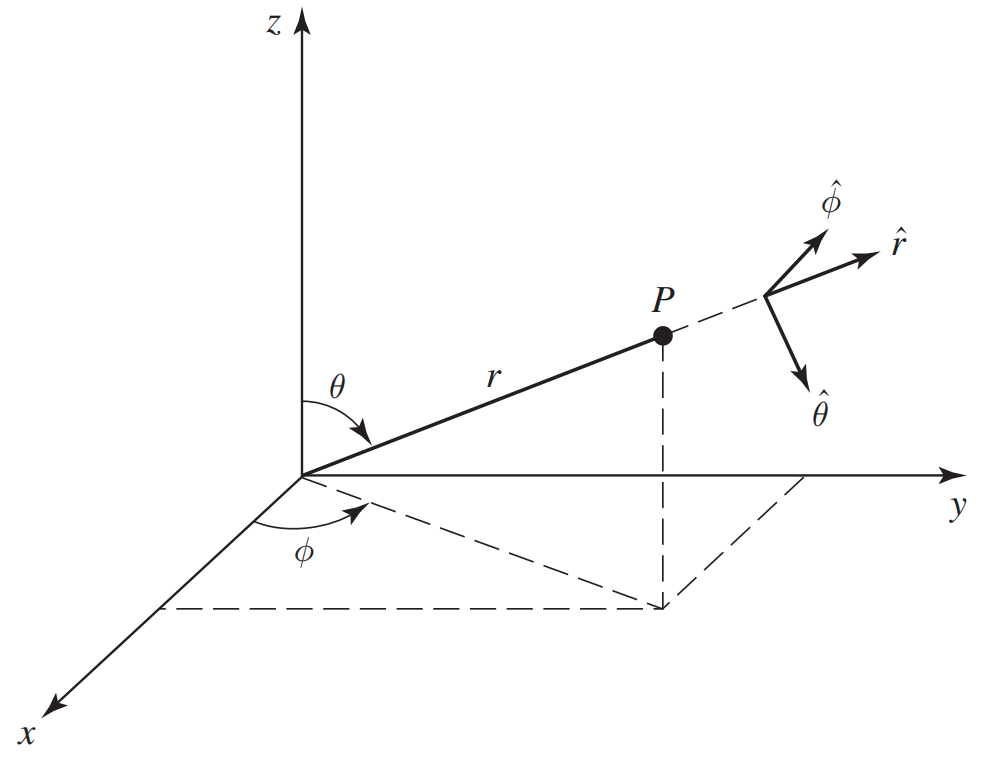
\includegraphics[width=0.48\textwidth]{figs/2022-03-28-22-51-18.png}
	\end{center}
\end{frame}

\begin{frame}
	  \frametitle{}	  
	\alert{解:}  坐标变换关系为:\\
	$\begin{cases}
		x= r\sin \theta \cos \varphi \\
		y= r\sin \theta \sin \varphi \\
		z=r\cos \theta
	\end{cases} $ \\
	对函数$u(x,y,z)$,进行 $r, \theta, \varphi $求导,有:\\ \vspace{0.6em}
	{\small $\begin{cases}
		\dfrac{\partial {u}}{\partial {r}}=\dfrac{\partial {u}}{\partial x} \dfrac{\partial {x}}{\partial {r}}+\dfrac{\partial u}{\partial {y}} \dfrac{\partial {y}}{\partial {r}}+\dfrac{\partial u}{\partial z} \dfrac{\partial z}{\partial {r}} \\ \vspace{0.3em}
		\dfrac{\partial {u}}{\partial \theta}=\dfrac{\partial {u}}{\partial x} \dfrac{\partial{x}}{\partial \theta}+\dfrac{\partial u}{\partial {y}} \dfrac{\partial {y}}{\partial \theta}+\dfrac{\partial{u}}{\partial z} \dfrac{\partial z}{\partial \theta} \\ \vspace{0.3em}
		\dfrac{\partial {u}}{\partial \varphi}=\dfrac{\partial u}{\partial x} \dfrac{\partial{x}}{\partial \varphi}+\dfrac{\partial u}{\partial y} \dfrac{\partial y}{\partial \varphi}+\dfrac{\partial u}{\partial z} \dfrac{\partial z}{\partial \varphi}
	\end{cases} $}\\ \vspace{1em}
\end{frame}	

\begin{frame}
	写成矩阵形式 \\ \vspace{1em}
	{\small $\left[\begin{array}{ccc}
		\dfrac{\partial u}{\partial r} \\ \vspace{0.3em}
		\dfrac{\partial u}{\partial \theta} \\ \vspace{0.3em}
		\dfrac{\partial u}{\partial \varphi}
	\end{array}\right]$
	=
	$\left[\begin{array}{ccc}
		\sin \theta \cos \varphi & \sin \theta \sin \varphi & \cos \theta \\ \vspace{0.3em}
		r \cos \theta \cos \varphi & r \cos \theta \sin \varphi & -r \sin \theta \\ \vspace{0.3em}
		-r \sin \theta \sin \varphi & r \sin \theta \cos \varphi & 0
	\end{array}\right]$
	$\left[\begin{array}{ccc}
		\dfrac{\partial u}{\partial x} \\ \vspace{0.3em}
		\dfrac{\partial u}{\partial y} \\ \vspace{0.3em}
		\dfrac{\partial u}{\partial z}
	\end{array}\right]$
	}\\
	{\small $\left[\begin{array}{ccc}
		\dfrac{\partial u}{\partial r} \\ \vspace{0.3em}
		\dfrac{\partial u}{\partial \theta} \\ \vspace{0.3em}
		\dfrac{\partial u}{\partial \varphi}
	\end{array}\right]$
	=
	$\left[\begin{array}{ccc}
		1 & 0 & 0 \\ \vspace{0.3em}
		0 & r  & 0 \\ \vspace{0.3em}
		0 & 0 & r \sin \theta 
	\end{array}\right]$
	$\left[\begin{array}{ccc}
		\sin \theta \cos \varphi & \sin \theta \sin \varphi & \cos \theta \\ \vspace{0.3em}
		\cos \theta \cos \varphi & \cos \theta \sin \varphi & - \sin \theta \\ \vspace{0.3em}
		-\sin \varphi &  \cos \varphi & 0
	\end{array}\right]$
	$\left[\begin{array}{ccc}
		\dfrac{\partial u}{\partial x} \\ \vspace{0.3em}
		\dfrac{\partial u}{\partial y} \\ \vspace{0.3em}
		\dfrac{\partial u}{\partial z}
	\end{array}\right]$
	}
\end{frame}	

\begin{frame}
	\small {$
		\left[\begin{array}{ccc}
			\dfrac{\partial u}{\partial x} \\
			\dfrac{\partial u}{\partial y} \\
			\dfrac{\partial u}{\partial z}
		\end{array}\right]$
		=
		$\left[\begin{array}{ccc}
			\sin \theta \cos \varphi & \cos \theta \cos \varphi & -\sin \varphi \\
			\sin \theta \sin \varphi &  \cos \theta \sin \varphi &  \cos \varphi \\
			\cos \theta & -\sin \theta & 0
		\end{array}\right]$
		$\left[\begin{array}{ccc}
			\dfrac{\partial u}{\partial r} \\
			\dfrac{1}{r}\dfrac{\partial u}{\partial \theta} \\
			\dfrac{1}{r \sin \theta}\dfrac{\partial u}{\partial \varphi}
		\end{array}\right]
		$}	\\ \vspace{0.3cm}
	\small {$
		\left[\begin{array}{ccc}
			\dfrac{\partial u}{\partial x} \\
			\dfrac{\partial u}{\partial y} \\
			\dfrac{\partial u}{\partial z}
		\end{array}\right]$
		=
		$\left[\begin{array}{ccc}
			{\vec{e}_r}&  {\vec{e}_\theta} & {\vec{e}_\varphi}
		\end{array}\right]$
		$\left[\begin{array}{ccc}
			\dfrac{\partial u}{\partial r} \\
			\dfrac{1}{r}\dfrac{\partial u}{\partial \theta} \\
			\dfrac{1}{r \sin \theta}\dfrac{\partial u}{\partial \varphi}
		\end{array}\right]
		$}	\\ 
\end{frame}	

\begin{frame}
	球坐标系下, 有:
	\begin{equation*}
	\nabla=\vec{e}_{r} \frac{\partial}{\partial r}+\frac{1}{r} \vec{e}_{\theta} \frac{\partial}{\partial \theta}+\frac{1}{r \sin \theta} \vec{e}_{\varphi} \frac{\partial}{\partial \varphi}
	\end{equation*}
	\begin{equation*}
	\begin{split}
		\nabla ^2&=\nabla \cdot \nabla \\
		&=(\vec{e}_{r} \frac{\partial}{\partial r}+\frac{1}{r} \vec{e}_{\theta} \frac{\partial}{\partial \theta}+\frac{1}{r \sin \theta} \vec{e}_{\varphi} \frac{\partial}{\partial \varphi})  \cdot (\vec{e}_{r} \frac{\partial}{\partial r}+\frac{1}{r} \vec{e}_{\theta} \frac{\partial}{\partial \theta}+\frac{1}{r \sin \theta} \vec{e}_{\varphi} \frac{\partial}{\partial \varphi}) \\
		&=\frac{\partial ^2}{\partial r^2} + ( \frac{1}{r} \frac{\partial}{\partial r} + \frac{1}{r^2} \frac{\partial^2} {\partial \theta ^2}  ) + (\frac{1}{r} \frac{\partial}{\partial r}  + \frac{\cos \theta}{r^2 \sin \theta} \frac{\partial} {\partial \theta }  + \frac{1}{r^2 \sin^2 \theta  } \frac{\partial^2}{\partial\varphi ^2} )\\
		&=\frac{1}{r^2} \frac{\partial }{\partial r} (r^2\frac{\partial }{\partial r} )+
		\frac{1}{r^2 \sin \theta  } \frac{\partial }{\partial \theta } (\sin \theta \frac{\partial }{\partial \theta } )
		+\frac{1}{r^2 \sin^2 \theta  } \frac{\partial^2}{\partial\varphi ^2}
	\end{split}
	\end{equation*}

	{\Bullet}~利用球坐标单位矢(1)正交归一性和(2)微分性质完成计算(见讲义 15页)
\end{frame}	

\begin{frame}
	直角坐标~ $(x,y,z) $: 
	\begin{equation*}
		\nabla ^{2}  = \dfrac{\partial ^2}{\partial x^2} +\dfrac{\partial^2 }{\partial y^2} +\dfrac{\partial^2  }{\partial z^2}
	\end{equation*}
	球坐标~ $(r,\theta, \varphi )$ :
	\begin{equation*}
		\nabla ^{2} =\frac{1}{r^2} \frac{\partial }{\partial r} (r^2\frac{\partial }{\partial r} )+
		\frac{1}{r^2 \sin \theta  } \frac{\partial }{\partial \theta } (\sin \theta \frac{\partial }{\partial \theta } )
		+\frac{1}{r^2 \sin^2 \theta  } \frac{\partial^2}{\partial\varphi ^2}
	\end{equation*}	
	令角向部分为:
	\begin{equation*}
		L^2 = - \left[ \frac{1}{ \sin \theta  } \frac{\partial }{\partial \theta } (\sin \theta \frac{\partial }{\partial \theta } )
		+\frac{1}{ \sin^2 \theta  } \frac{\partial^2}{\partial\varphi ^2} \right]
	\end{equation*}	
	有 :
	\begin{equation*}
		\nabla ^{2} =\frac{1}{r^2} \frac{\partial }{\partial r} (r^2\frac{\partial }{\partial r} )-
		\frac{1}{r^2 } L^2 
	\end{equation*}	
	的确它由径向和角向二部分加和构成,因此可实现径向和角向的分离变量!
\end{frame}	

\begin{frame}
	\frametitle{角向与角动量的关系}	
	角向(方)算子:
	\begin{equation*}
		L^2 = - \left[ \frac{1}{ \sin \theta  } \frac{\partial }{\partial \theta } (\sin \theta \frac{\partial }{\partial \theta } )
		+\frac{1}{ \sin^2 \theta  } \frac{\partial^2}{\partial\varphi ^2} \right]
	\end{equation*}	
    角动量(方)算子:
		\begin{equation*}
		L^2 = -\hbar ^2 \left[ \frac{1}{ \sin \theta  } \frac{\partial }{\partial \theta } (\sin \theta \frac{\partial }{\partial \theta } )
		+\frac{1}{ \sin^2 \theta  } \frac{\partial^2}{\partial\varphi ^2} \right]
	\end{equation*}	
	动量的切向分量
	\begin{equation*}
	p_ \perp  ^2 =  \frac{L^2}{r^2}
	\end{equation*}	
	动量的径向分量
	\[ p_r ^2 = -\hbar ^2  \frac{1}{r^2} \frac{\partial }{\partial r} (r^2\frac{\partial }{\partial r} ) \]
\end{frame}		

\begin{frame}
	得动量算子: 
	\[ \hspace{1em}\hat{p}^2 =-\hbar ^2 \nabla ^{2}
		\]
	\[ \hat{p} =-i\hbar \nabla \quad \text{or} \quad i\hbar \nabla\]
	在球坐标系下,
	\[ \hat{p} =-i\hbar  ( \vec{e}_{r} \frac{\partial}{\partial r}+\frac{1}{r} \vec{e}_{\theta} \frac{\partial}{\partial \theta}+\frac{1}{r \sin \theta} \vec{e}_{\varphi} \frac{\partial}{\partial \varphi})
		\]
\end{frame}		

\begin{frame}
	\frametitle{位置算子 }	
	$\begin{cases}
		x= r\sin \theta \cos \varphi \\
		y= r\sin \theta \sin \varphi \\
		z=r\cos \theta
	\end{cases} $\\ 
	~~\\
	矩阵形式: \\ \vspace{0.6em}
	$
	\left[\begin{array}{ccc}
		x \\
		y \\
		z
	\end{array}\right]$
	=
	$\left[\begin{array}{ccc}
		r\sin \theta \cos \varphi  \\
		r\sin \theta \sin \varphi  \\
		r\cos \theta
	\end{array}\right]$	
	=
	$r \vec{e}_r$ \\ \vspace{0.3cm}
	球坐标系下,位置算子:
	\[ \qquad \hat{r}=r \vec{e}_r \]
\end{frame}	

\begin{frame}
	角动量: $ \vec{L}= \vec{r}\times \vec{p} $, \\
	球坐标系下,角动量算子:
	\begin{equation*}
		\hat{L}= \hat{r}\times \hat{p} = -i \hbar r \vec{e}_r \times \nabla  
	\end{equation*}
	\begin{equation*}
		\hat{L}=   -i \hbar   ( \vec{e}_{\varphi} \frac{\partial}{\partial \theta} - \frac{1}{\sin \theta}  \vec{e}_{\theta} \frac{\partial}{\partial \varphi} )
	\end{equation*}
	\begin{equation*}
		\begin{split}
		\hat{L}	^2 &=   - \hbar ^2  ( e_{\varphi} \frac{\partial}{\partial \theta} - \frac{1}{\sin \theta}  e_{\theta} \frac{\partial}{\partial \varphi} )  \cdot   ( e_{\varphi} \frac{\partial}{\partial \theta} - \frac{1}{\sin \theta}  e_{\theta} \frac{\partial}{\partial \varphi} ) \\
		&= - \hbar ^2 (\frac{1}{\sin \theta  } \frac{\partial }{\partial \theta } (\sin \theta \frac{\partial }{\partial \theta } )
		+\frac{1}{\sin^2 \theta  } \frac{\partial^2}{\partial\varphi ^2} ) 	
		\end{split}
	\end{equation*}
	正是前面的假设, 完全自洽!\\ \vspace{1em}

	同样, 可得到角动量的Z分量 (不证):
	\begin{equation*}
		\hat{L}_z= -i \hbar \frac{\partial }{\partial\varphi }
	\end{equation*}	
\end{frame}	

%#############################################
\subsection{球坐标系氢原子方程 }	

\begin{frame}
	\frametitle{ 球坐标系氢原子方程 }	
	球坐标下的哈密顿量 (折合质量$m$计为 $\mu$):
	\begin{equation*}
		\begin{split}
		H&=-\frac{\hbar^2}{2 \mu r^2}  \frac{\partial }{\partial r} (r^2\frac{\partial }{\partial r} ) +  \frac{\hbar^2}{2 \mu r^2} L^2  -\frac{e_s ^2}{r} \\
		&= \frac{1}{2 \mu } p_r ^2 +  \frac{1}{2 \mu r^2} L^2  -\frac{e_s ^2}{r} 	
		\end{split}	
	\end{equation*}	
	球坐标系氢原子定态方程:	
	\begin{equation*}
		\left[ (\frac{1}{2 \mu } p_r ^2  -\frac{e_s ^2}{r})  +\frac{1}{2 \mu }	p_ \perp  ^2   \right] \Psi (r,\theta,\varphi) =E \Psi (r,\theta,\varphi)  
	\end{equation*}	
	方程可做动量的径向/切向分离.......\\
\end{frame}		

\begin{frame}
	为了与数学方程统一,先不考虑物理意义,仅采用角向(方)算子 $L^2$(与角动量(方)算子差~$\hbar ^2$):
	\begin{equation*}
		L^2 =  -\left[ \frac{1}{ \sin \theta  } \frac{\partial }{\partial \theta } (\sin \theta \frac{\partial }{\partial \theta } )
		+\frac{1}{ \sin^2 \theta  } \frac{\partial^2}{\partial\varphi ^2} \right]
	\end{equation*}	
	球坐标系下的方程为:
	\begin{equation*}
		\left[-\frac{\hbar^2}{2 \mu r^2}  \frac{\partial }{\partial r} (r^2\frac{\partial }{\partial r} ) +  \frac{\hbar ^2 }{2 \mu r^2} L^2  -\frac{e_s ^2}{r} \right] \Psi
		=E\Psi
	\end{equation*}	
	数学上的径向/角向分离变量,令: 
	\begin{equation*}
		\Psi=R (r) Y(\theta,\varphi)
	\end{equation*}	
	代回原方程,得:
	\begin{equation*}
		\frac{ L^2 Y}{Y}= \frac{1}{R}   \frac{\partial }{\partial r} (r^2\frac{\partial R }{\partial r} ) + \frac{2 \mu r^2} {\hbar^2}(E+ \frac{e_s ^2}{r} )=\lambda
	\end{equation*}	
\end{frame}		

\begin{frame}
	氢原子的定态方程在球坐标系下变量分离,得两个方程:	\\
	(1)角向方程:
	\begin{equation*}
		L^2 Y=\lambda Y
	\end{equation*}	
	(2)径向方程:
	\begin{equation*}
		\frac{d}{d r} (r^2\frac{d R }{d r} ) + \frac{2 \mu r^2} {\hbar^2}(E+ \frac{e_s ^2}{r} ) R =\lambda R
	\end{equation*}	
	下面分别求解数学上的角向/径向方程...
\end{frame}	

\begin{frame}
	\frametitle{ 作业 }
	1、求基向量($\vec{e}_r, \vec{e}_\theta, \vec{e}_\varphi$) 点积和叉积的运算规律\\
	2、求如下偏分
	\begin{equation*}
	\frac{\partial }{\partial \theta}  e_\theta, \qquad \frac{\partial }{\partial \theta}  e_r 
	\end{equation*}	
    3、角向算子与角动量算子有什么区别? \\
	4、为什么只有氢原子薛定谔方程可以精确求解?
\end{frame}	
%%%%%%%%%%%%%%%%%%%%%%%%%%%%%%%%%%%%%%%%%%%%%%

\section{2.角向方程与勒让德多项式}

\subsection{ 经/纬分离}

\begin{frame}
	\frametitle{角向方程分离变量}
	(1)角向方程:
	\begin{equation*}
		L^2 Y=\lambda Y
	\end{equation*}	
	令 $\lambda=l(l+1) $ 课外参考 \href{https://zhuanlan.zhihu.com/p/133865994}{点这里}
	\begin{equation*}
		L^2 Y=l(l+1) Y
	\end{equation*}	
	代入角向算子:
	\begin{equation*}
		\left[ \frac{1}{ \sin \theta  } \frac{\partial }{\partial \theta } (\sin \theta \frac{\partial }{\partial \theta } )
		+\frac{1}{ \sin^2 \theta  } \frac{\partial^2}{\partial\varphi ^2}  +l(l+1) \right] Y=0 
	\end{equation*}	
	方程可进一步分离变量,令:
	\begin{equation*}
		Y(\theta,\varphi)= \Theta(\theta) \Phi(\varphi)
	\end{equation*}	
	代回上方程,得:
\end{frame}	

\begin{frame}
	\begin{equation*}
		\Phi \frac{1}{\sin \theta} \frac{d}{d \theta}\left(\sin \theta \frac{d \Theta}{d \theta}\right)+\Theta \frac{1}{\sin ^{2} \theta} \frac{d^{2} \Phi}{d \varphi^{2}}+l(l+1) \Theta \Phi=0
	\end{equation*}	
	整理:
	\begin{equation*}
		\frac{\sin ^{2} \theta}{\Theta \sin \theta} \frac{d}{d \theta}\left(\sin \theta \frac{d \Theta}{d \theta}\right)+\sin ^{2} \theta l(l+1)=-\frac{1}{\Phi} \frac{d^{2} \Phi}{d \varphi^{2}}=\lambda
	\end{equation*}	
	(1)经度方程:
	\begin{equation*}
		\frac{d^{2} \Phi}{d \varphi^{2}}+\lambda \Phi=0,(0<\varphi\le2 \pi)
	\end{equation*}	
	(2)纬度方程:
	\begin{equation*}
		\frac{1}{\sin \theta} \frac{d}{d \theta}\left(\sin \theta \frac{d \Theta}{d \theta}\right)+\left[l(l+1)-\frac{\lambda}{\sin ^{2} \theta}\right] \Theta=0,(0<\theta \le \pi)
	\end{equation*}	
\end{frame}	

\subsection{解经度方程}

\begin{frame}
	\frametitle{解经度方程}
	经度方程是周期性边界条件下的固有值问题:\\
	\[\begin{cases}
		\dfrac{d^{2} \Phi}{d \varphi^{2}}+\lambda \Phi=0,0<\varphi<2 \pi \\ 
		\Phi(0)=\Phi(2 \pi), \Phi^{\prime}(0)=\Phi^{\prime}(2 \pi)
	\end{cases}\]
	
	特征方程有两虚根,对应固有值和固有函数为:
	\[\begin{cases}
		\lambda=m^2, ~~~ (m=0,\pm 1,\pm 2,\cdots) \\ 
		\Phi_m (\varphi)=A\cos m\varphi+B\sin m\varphi
	\end{cases}\]
	
	指数形式
	\begin{equation*}
		\Phi_m (\varphi)=A_m e^{im\varphi}
	\end{equation*}	
\end{frame}	

\begin{frame}
	求归一化系数 :
	\begin{equation*}
	\begin{split}
		\int_{0}^{2\pi}  |\Phi_m (\varphi)|^2 d\varphi &= 1 \\
		\int_{0}^{2\pi}  A_m e^{im\varphi} A_m e^{-im\varphi} d\varphi &= 1 \\
		A^2_m \int_{0}^{2\pi} 1 d\varphi &= 1 \\
		A^2_m 2\pi &= 1 \\
		A_m&=\frac{1}{\sqrt{2\pi}} 
	\end{split}
	\end{equation*}	
	\begin{equation*}
	\to 	\Phi_m (\varphi)=\frac{1}{\sqrt{2\pi}} e^{im\varphi}
	\end{equation*}	
\end{frame}	

\subsection{解纬度方程}
\begin{frame}
	\frametitle{解纬度方程}
	把固有值$\lambda=m^2$代回纬度方程,得m阶连带勒让德方程:
	\begin{equation*}
		\boxed{\frac{1}{\sin \theta} \frac{d}{d \theta}\left(\sin \theta \frac{d \Theta}{d \theta}\right)+\left[l(l+1)-\frac{m^{2}}{\sin ^{2} \theta}\right] \Theta=0}
	\end{equation*}	
	\alert{解:}~微分展开,得:
	\begin{equation*}
		\frac{d^{2} \Theta}{d \theta^{2}}+\frac{\cos \theta}{\sin \theta} \frac{d \Theta}{d \theta}+\left[l(l+1)-\frac{m^{2}}{\sin ^{2} \theta}\right] \Theta=0
	\end{equation*}		
	(勒让德)令:$x=\cos \theta$,  $y(x)= y(\cos \theta) =\Theta (\theta)$, 有:
	\begin{equation*}
		\frac{d x}{d  \theta} =-\sin \theta  
	\end{equation*}		
	\begin{equation*}
		\frac{d \Theta}{d \theta} =\frac{d y}{d x}\frac{d x}{d \theta} =-\sin \theta \frac{d y}{d x}
	\end{equation*}		
\end{frame}	

\begin{frame}
	\begin{equation*}
		\frac{ d^2 \Theta }{d \theta ^2} =\sin ^2 \theta \frac{d^2 y}{d x^2} -\cos \theta \frac{d y}{d x}
	\end{equation*}		
	代回方程,注意($\cos\theta =x,~ \sin  \theta =1-x^2 $), \\
	得标准连带勒让德方程:
	\begin{equation*}
		\left(1-x^{2}\right) \frac{d^{2} y}{d x^{2}}-2 x \frac{d y}{d x}+\left[l(l+1)-\frac{m^{2}}{1-x^{2}}\right] y=0, \quad (|x|\le 1)
	\end{equation*}		
	若 m=0,就是(0阶)勒让德方程:
	\begin{equation*}
		\left(1-x^{2}\right) \frac{d^{2} y}{d x^{2}}-2 x \frac{d y}{d x}+l(l+1)y=0
	\end{equation*}		
\end{frame}	

\subsection{解勒让德方程}

\begin{frame}
	\frametitle{解勒让德方程}
	\begin{equation*}
		\boxed{\left(1-x^{2}\right) \frac{d^{2} y}{d x^{2}}-2 x \frac{d y}{d x}+l(l+1)y=0}
	\end{equation*}		
	\alert{解:} (勒让德)令方程有级数解,
	\[ y=\sum_{k=0}^{\infty} a_k x ^k \]
	求导,并代回方程,得:
	\begin{equation*}
		\sum_{k=0}^{\infty}\left\{(k+1)(k+2) a_{k+2}+[l(l+1)-k(k+1)] a_{k}\right\} x^{k}=0
	\end{equation*}	
	系数项为零:
	\begin{equation*}
		(k+1)(k+2) a_{k+2}+[l(l+1)-k(k+1)] a_{k}=0
	\end{equation*}	   
\end{frame}	

\begin{frame}
	得递推式:
	\begin{equation*}
		a_{k+2}=-\frac{(l-k)(l+k+1)}{(k+1)(k+2) }a_{k}
	\end{equation*}	   
	k为偶数:
	\begin{equation*}
		y_{1}(x)=\left[1-\frac{l(l+1)}{2} x^{2}+\frac{l(l+1)(l+3)(l-2)}{4 !} x^{4}+\cdots\right]
	\end{equation*}	
	k为奇数:
	\begin{equation*}
		y_{2}(x)=\left[x-\frac{(l-1)(l+2)}{3 !} x^{3}+\frac{(l+2)(l+3)(l-1)(l-3)}{5 !} x^{5}+\cdots\right]
	\end{equation*}	    
	方程的级数解:\[ y(x)=  a_{0}y_{1}(x) + a_{1} y_{2}(x)  \]	
\end{frame}	

\begin{frame}
	\frametitle{}
	\begin{equation*}
		a_{k+2}=-\frac{(l-k)(l+k+1)}{(k+1)(k+2) }a_{k}
	\end{equation*}
	说明存在最高项$k=l$ \\
	逆向递推式为 
	\begin{equation*}
		a_{k}=-\frac{(k+1)(k+2) }{(l-k)(l+k+1)}a_{k+2}
	\end{equation*}	   
	{\Bullet}逆向递推式
	\begin{equation*}
		a_{k-2}=-\frac{(k-1)(k) }{(l-k+2)(l+k-1)}a_{k}
	\end{equation*}	    
	注意到级数最高项 $k=l$,现以$n$描述, 有 
	\begin{equation*}
		a_{n-2}=-\frac{(n-1) n}{2(2n-1)} a_{n}
	\end{equation*}	 
\end{frame}	

\begin{frame}
	令最高项系数: \[a_n=\frac{(2n)!}{2^n (n!)^2} = \frac{(2n-2)!\times 2n \times (2n-1)}{2^n (n-1)!\times n \times (n-2)!\times n \times (n-1)  } \]
	得逆向递推式:
	\begin{equation*}
		a_{n-2}=-\frac{(2 n-2) !}{2^{n} 1! (n-1) !(n-2) !}
	\end{equation*}	 
	\begin{equation*}
		a_{n-2\times2}=(-)^2\frac{(2 n-2\times2) !}{2^{n} 2! (n-2) !(n-2\times2) !}
	\end{equation*}	 
	一般式:
	\begin{equation*}
		a_{n-2 m}=(-1)^{m} \frac{(2 n-2 m) !}{2^{n} m !(n-m) !(n-2 m) !}
	\end{equation*}	 
\end{frame}	

\begin{frame}
	得勒让德方程的多项式解:
	\begin{equation*}
		y(x)=\sum_{k=0}^{\infty}a_k x^k =\sum_{m=0}^{[n / 2]}(-1)^{m} \frac{(2 n-2 m) !}{2^{n} m !(n-m) !(n-2 m) !} x^{n-2 m}=P_{n}(x)
	\end{equation*}	 
	TIPS 指标计算:
	\[ k=n-2m \]
	\[k=0, \to  m=[n/2] \]
	\[k=l=n, \to m=0 \]
	称此多项式为勒让德多项式$P_n(x)$, 即 $P_l(x)$。
\end{frame}	

\subsection{勒让德多项式及其性质}

\begin{frame}
	\frametitle{勒让德多项式}
	\[P_{n}(x)=\sum_{m=0}^{[n / 2]}(-1)^{m} \frac{(2 n-2 m) !}{2^{n} m !(n-m) !(n-2 m) !} x^{n-2 m}\]
	\[ n=0, m=[n/2]=0; \qquad n=1, m=[n/2]=0; \qquad n=2, m=0,1 ; \cdots \hspace{5em}\]
	取 x=$\cos\theta$,得下表右列:\\ \vspace{0.3em}
	{\small $\begin{array}{|l|l|}
		\hline P_{0}(x)=1 & P_{0}(\cos\theta)=1\\
		\hline P_{1}(x)=x & P_{1}(\cos \theta)=\cos \theta \\
		\hline P_{2}(x)=\dfrac{1}{2}\left(3 x^{2}-1\right) & P_{2}(\cos \theta)=\dfrac{1}{4}[3 \cos 2 \theta+1] \\ 
		\hline P_{3}(x)=\dfrac{1}{2}\left(5 x^{3}-3 x\right) & P_{3}(\cos \theta)=\dfrac{1}{8}[5 \cos 3 \theta+3 \cos \theta] \\
		\hline P_{4}(x)=\dfrac{1}{8}\left(35 x^{4}-30 x^{2}+3\right) & P_{4}(\cos \theta)=\dfrac{1}{64}[35 \cos 4 \theta+20 \cos 2 \theta+9] \\
		\hline
	\end{array}$}
\end{frame}	 

\begin{frame}
	\frametitle{勒让德多项式性质}
	\alert{性质1}:勒让德多项式有如下微分形式:
	\begin{equation*}
		P_{n}(x)=\frac{1}{2^{n} n !} \frac{d^{n}}{d x^{n}}\left(x^{2}-1\right)^{n}, \quad(n=0,1,2,3, \cdots \cdots)
	\end{equation*}	 
	\alert{证明:} 由二项式定理,有:
	\begin{align*}
		\left(x^{2}-1\right)^{n}&=\sum_{m=0}^{n} C_{n}^{m}(-1)^{m}\left(x^{2}\right)^{n-m}\\
		&=\sum_{m=0}^{n} \frac{(-1)^{m} n !}{m !(n-m) !} x^{2 n-2 m}
	\end{align*}	 
	求n次导,
	\begin{equation*}
		\frac{d^{n}}{d x^{n}}\left(x^{2}-1\right)^{n}=\sum_{m=0}^{n} \frac{(-1)^{m} n !}{m !(n-m) !} \frac{d^{n}}{d x^{n}}\left(x^{2 n-2 m}\right)
	\end{equation*}	
\end{frame}	

\begin{frame}
	当$2n-2m<n$时, 上次的右边导数为零,即非零的最高项为 $[n/2]$,  有:
	\begin{align*}
		\frac{d^{n}}{d x^{n}}\left(x^{2}-1\right)^{n}&=\sum_{m=0}^{[n/2]} \frac{(-1)^{m} n !}{m !(n-m) !} \frac{d^{n}}{d x^{n}}\left(x^{2 n-2 m}\right)\\
		&=\sum_{m=0}^{[n / 2]}(-1)^{m} \frac{(2 n-2 m) ! n!}{ m !(n-m) !(n-2 m) !} x^{n-2 m}\\
	\end{align*}	
	\begin{align*}
		\frac{1}{2^{n} n !} \frac{d^{n}}{d x^{n}}\left(x^{2}-1\right)^{n} &= \sum_{m=0}^{[n / 2]}(-1)^{m} \frac{(2 n-2 m) !}{2^{n} m !(n-m) !(n-2 m) !} x^{n-2 m}\\
		&=P_n(x)\\
	\end{align*}	
	\alert{证毕!}
\end{frame}	

\begin{frame}
	\alert{性质2:}勒让德多项式具有如下母函数:
	\begin{equation*}
		w(x, z)=\left(1-2 z x+z^{2}\right)^{-1 / 2}
	\end{equation*}	
	\alert{证明:}即要证
	\begin{equation*}
		\left(1-2 z x+z^{2}\right)^{-1 / 2}=\sum_{n=0}^{\infty} P_n(x) z^n
	\end{equation*}	
	由二项式定理有:
	\begin{equation*}
		(1+v)^{p}=\sum_{k=0}^{\infty} \frac{p(p-1) \cdots(p-k+1)}{k !} v^{k}
	\end{equation*}	
\end{frame}	

\begin{frame}
	取$p=-1/2$, 得:
	\begin{align*}
		(1+v)^{-1/2}&=\sum_{k=0}^{\infty} (-1)^{k}\frac{\frac{1}{2}\frac{3}{2}  \cdots \frac{2k-1}{2}}{k !} v^{k}\\
		&=\sum_{k=0}^{\infty} (-1)^{k}\frac{\frac{1}{2}\frac{2}{2}\frac{3}{2} \frac{4}{2}  \cdots \frac{2k-1}{2}\frac{2k}{2}} {(k !)^2} v^{k}\\
		&=\sum_{k=0}^{\infty}(-1)^{k} \frac{(2 k) !}{2^{2 k}(k !)^{2}} v^{k}
	\end{align*}	
	取$v=-2zx+z^2=-z(2x-z)$, 有:
	\begin{equation*}
		v^{k}=(-1)^{k} z^{k}(2 x-z)^{k}=(-1)^{k} z^{k} \sum_{m=0}^{k} C_{k}^{m}(2 x)^{k-m}(-z)^{m}
	\end{equation*}	
	代回
	\begin{equation*}
		\left(1-2 z x+z^{2}\right)^{-\frac{1}{2}}=\sum_{k=0}^{\infty} \frac{(2 k) !}{2^{2 k}(k !)^{2}} \sum_{m=0}^{k}(-1)^{m} C_{k}^{m}(2 x)^{k-m} z^{k+m}
	\end{equation*}	
\end{frame}	

\begin{frame}
	令:$k+m=n$,则有关$z^{n}$的展开系数为
	\begin{equation*}
	\begin{split}
		\sum_{k+m=n}\frac{(2 k) !}{2^{2 k}(k !)^{2}} & (-1)^{m} C_{k}^{m}(2 x)^{k-m}\\
		&=\sum_{m=0}^{n} \frac{(2 (n-m)) !}{2^{2 (n-m)}((n-m) !)^{2}}(-1)^{m} C_{n-m}^{m}(2 x)^{n-2m}\\
		&=\sum_{m=0}^{n}(-1)^{m} \frac{(2 n-2m) !}{2^{2 (n-m)}((n-m) !)^{2}} \frac{(n-m) !}{m!(n-2 m) !}2^{n-2 m}x^{n-2 m}\\
		&=\sum_{m=0}^{n}(-1)^{m} \frac{(2 n-2 m) !}{2^{n} m !(n-m) !(n-2 m) !} x^{n-2 m} \\
		&=P_{n}(x)
	\end{split}
	\end{equation*}	
	\alert{证毕!}
\end{frame}	

\begin{frame}
	\alert{性质3:}勒让德多项式具有如下递推关系:
	\begin{equation*}
		(n+1) P_{n+1}(x)-(2 n+1) x P_{n}(x)+n P_{n-1}(x)=0
	\end{equation*}	
	\alert{证明:} 对于母函数的形式级数:
	\begin{equation*}
		w(x, z)=(1-2zx+z^2{-1/2})=\sum_{n=0}^{\infty} P_{n}(x) z^{n}
	\end{equation*}	
	求关于z的偏导:
	\begin{equation*}
		\frac{\partial w}{\partial z}=\sum_{n=1}^{\infty} n P_{n}(x) z^{n-1}=\sum_{n=0}^{\infty}(n+1) P_{n+1} z^{n}
	\end{equation*}		
\end{frame}	

\begin{frame}
	\begin{equation*}
		\frac{\partial w}{\partial z}=	(x-z)(1-2zx+z^2){-3/2}
	\end{equation*}		
	\begin{equation*}
		(1-2zx+z^2)\frac{\partial w}{\partial z}=(x-z)(1-2zx+z^2){-1/2}
	\end{equation*}		
	\begin{equation*}
		(1-2zx+z^2)\frac{\partial w}{\partial z}-(x-z)w=0
	\end{equation*}		
	\begin{equation*}
		(1-2zx+z^2)\sum_{n=0}^{\infty}(n+1) P_{n+1} z^{n}-(x-z)\sum_{n=0}^{\infty} P_{n}(x) z^{n}=0
	\end{equation*}		
	整理,得
	\begin{equation*}
		\sum_{n=1}^{\infty} [(n+1)P_{n+1} -(2n+1)x P_n + nP_{n-1} ] z^{n}=0
	\end{equation*}		
	系数项等于零,\alert{得证!}   	  
\end{frame}	

\begin{frame}
	\alert{性质4:}~勒让德多项式具有正交性:\\
	\alert{证明:}  勒让德多项式满足勒让德方程($n=l$)
	\begin{equation*}
		\left(1-x^{2}\right) P'' _n  (x) -2 x P' _n (x)+n(n+1)P_n(x)=0
	\end{equation*}		
	等价形式:
	\begin{equation*}
		[\left(1-x^{2}\right) P' _n  (x)]' +n(n+1)P_n(x)=0    \cdots  (1)
	\end{equation*}		
	同理:
	\begin{equation*}
		[\left(1-x^{2}\right) P' _m  (x)]' + m (m+1)P_m(x)=0    \cdots  (2)
	\end{equation*}		
	(1)式$\times P_m$, (2)式$\times P_n$,所得两式相减并积分: 
	{\small \begin{equation*}
			[n(n+1) -m (m+1)]\int_{-1}^{1} P_mP_n dx =\int_{-1}^{1} (P_n [\left(1-x^{2}\right) P' _m] '-P_m [\left(1-x^{2}\right) P' _n ]')dx
	\end{equation*}		}
\end{frame}	

\begin{frame}
	上式右端分部积分,
	\begin{equation*}
	\begin{split}
		= &(P_n [\left(1-x^{2}\right) P' _m] - P_m [\left(1-x^{2}\right) P' _n ])|_{-1} ^{1} \\ 
		&-\int_{-1}^{1}  [\left(1-x^{2}\right) P' _nP' _m -\left(1-x^{2}\right) P' _mP' _n  ]  dx \\
		=&0
	\end{split}
	\end{equation*}		
	因此,式子的左端
	\begin{equation*}
		[n(n+1) -m (m+1)]\int_{-1}^{1} P_mP_n dx =0
	\end{equation*}	
	有:
	\begin{equation*}
		\int_{-1}^{1} P_mP_n dx =0 ,\cdots (n\ne m)
	\end{equation*}	
	\alert{证毕!} 
\end{frame}	

\begin{frame}
	\alert{性质5:} 勒让德多项式平方可积
	\begin{equation*}
		\int_{-1}^{1} P_nP_n dx = \frac{2}{2n+1}
	\end{equation*}	
	\alert{证明:}  由递推公式
	\begin{equation*}
		nP_{n} -(2n-1)x P_{n-1} + (n-1)P_{n-2}  =0
	\end{equation*}		
	\begin{equation*}
		nP ^2 _{n} =(2n-1)x P_n P_{n-1} - (n-1)P_nP_{n-2} 
	\end{equation*}		
	\begin{equation*}
		\int_{-1}^{1}  P ^2 _{n} dx = \frac{(2n-1)}{n} \int_{-1}^{1}  x P_n P_{n-1} dx , \cdots (1)
	\end{equation*}	
	递推式可写成
	\begin{equation*}
		(n+1)P_{n+1} -(2n+1)x P_{n} + nP_{n-1}  =0  
	\end{equation*}		
	\begin{equation*}	
		x P_{n}=\frac{n+1}{2n+1}P_{n+1} + \frac{n}{2n+1}P_{n-1} , \cdots (2)
	\end{equation*}	
	把(2)代入(1)式,
\end{frame}	

\begin{frame}	
	得积分递推式
	\begin{align*}
		\int_{-1}^{1}  P ^2 _{n} dx &=  \frac{2n-1}{2n+1}\int_{-1}^{1}   P^2_{n-1} dx \\
		&=  \frac{2n-1}{2n+1} \cdot \frac{2(n-1)-1}{2(n-1)+1} \int_{-1}^{1}   P^2_{n-2} dx \\
	\end{align*}		
	反复递推:
	\begin{equation*}
		\int_{-1}^{1}  P ^2 _{n} dx =  \frac{1}{2n+1}\int_{-1}^{1}   P^2_{0} dx = \frac{2}{2n+1}
	\end{equation*}		
	\alert{证毕!} 
\end{frame}	


\begin{frame}
	\alert{例 1:}	利用勒让德多项式正交性计算积分:
	\begin{equation*}
		\int_{-1}^{+1} x^2 P _{n}(x) dx 
	\end{equation*}		
	\alert{解:} 由 $ P_{n}(x)=\dfrac{1}{2^{n} n !} \dfrac{d^{n}}{d x^{n}}\left(x^{2}-1\right)^{n} $, 得:
	\begin{equation*}
		P_0(x)=1, 	P_1(x)=x,  P_2(x)= \dfrac{1}{2}(3x^2-1)  
	\end{equation*}	
	 $x^2$的勒让德多项式展开式:
	$$ x^2 =\dfrac{2}{3}P_2+\dfrac{1}{3}P_0$$
	原式为:
	\begin{equation*}
			\int_{-1}^{+1} x^2 P _{n} dx = \int_{-1}^{+1} (\dfrac{2}{3}P_2+\dfrac{1}{3}P_0)  P _{n} dx 	
	\end{equation*}	
\end{frame}	

\begin{frame}
	分情况讨论:\\
	(1)  $n=0$, 
	\begin{equation*}
		\int_{-1}^{+1} x^2 P _{n} dx  =   \int_{-1}^{+1} \dfrac{1}{3}P_0  P _{0} dx=\dfrac{1}{3} \frac{2}{2n+1}  = \dfrac{2}{3}	
	\end{equation*}	
	(2)  $n=2$, 
	\begin{equation*}
		\int_{-1}^{+1} x^2 P _{n} dx  =   \int_{-1}^{+1} \dfrac{2}{3}P_2  P _{2} dx= \dfrac{2}{3}\frac{2}{2n+1}  = \dfrac{4}{15}	
	\end{equation*}	
	(3) $ n\neq 0,2$
	\begin{equation*}
		\int_{-1}^{+1} x^2 P _{n} dx  =  0	
	\end{equation*}
\end{frame}	

\begin{frame}
	\frametitle{Tips:得记住}	
	\begin{equation*}
		\begin{split}
		1&= P_0 \\
		x&=P_1\\
	    x^2&=\dfrac{1}{3}(2P_2+P_0)\\
		x^3&=\dfrac{1}{5}(2P_3+3P_1)		
		\end{split}
	\end{equation*}
\end{frame}	

\subsection{连带勒让德多项式}

\begin{frame}
	\frametitle{连带勒让德多项式}
	勒让德方程:
	\begin{equation*}
		\left(1-x^{2}\right) \frac{d^{2} y}{d x^{2}}-2 x \frac{d y}{d x}+l(l+1)y=0
	\end{equation*}		
	解为勒让德多项式
	\begin{equation*}
		P_{l}(x)=\frac{1}{2^{l} l !} \frac{d^{l}}{d x^{l}}\left(x^{2}-1\right)^{l}, \quad(l=0,1,2,3, \cdots \cdots)
	\end{equation*}	 
	连带勒让德方程:
	\begin{equation*}
		\left(1-x^{2}\right) \frac{d^{2} y}{d x^{2}}-2 x \frac{d y}{d x}+\left[l(l+1)-\frac{m^{2}}{1-x^{2}}\right] y=0
	\end{equation*}		
	解为连带勒让德多项式
	\begin{equation*}
		P^m  _{l}(x)= (1-x^2) ^ {m/2 } \frac{d^{m}}{d x^{m} } P_l(x),  \quad(m < l, l=0,1,2,3, \cdots \cdots)
	\end{equation*}	 
\end{frame}	

\begin{frame}
	\frametitle{证明思路:}
	把勒让德多项式 $P_{l}(x) $ 代入勒让德方程,然后对勒让德方程逐级求导, m次后得连带勒让德方程
	\begin{equation*}
		\begin{split}
			&\left(1-x^{2}\right) P'' _l  (x) -2 x P' _l (x)+l(l+1)P_l(x)=0	\\
			&\left(1-x^{2}\right) P^{3} _l  (x) -2(1+1) x P'' _l (x)+(l(l+1)-1(1+1)P'_l(x)=0	\\
			&\left(1-x^{2}\right) P^{4} _l  (x) -2(2+1) x P^{3} _l (x)+(l(l+1)-2(2+1)P''_l(x)=0	\\
			& \cdots \cdots\\
			&\left(1-x^{2}\right) P^{m+2} _l  (x) -2(m+1) x P^{m+1} _l (x)+(l(l+1)-m(m+1)P^{m} _l(x)=0	\\
		\end{split}
	\end{equation*}
	即: 连带勒让德多项式  $P^{m} _l  (x)  $ 是连带勒让德方程的解,($m < l$)
\end{frame}	

\begin{frame}
	连带勒让德多项式性质:\\
	(1) 正交性: 
	\begin{equation*}
		\int_{-1}^{1} P^m _{l'}P^m _{l} dx =0 ,\cdots (l'\ne l)
	\end{equation*}	
	(2) 归一性:
	\begin{equation*}
		\int_{-1}^{1} P^m _l P^m _l dx =  \frac{(l+m)!}{(l-m)!}\frac{2}{2l+1}
	\end{equation*}	
	(3) 递推式: 
	\begin{equation*}
		(l+1-m)P^m _{l+1} -(2l+1)x P^m _l + (l+m) P^m _{l-1} =0 
	\end{equation*}		
\end{frame}	

\begin{frame}
	\frametitle{球谐函数}
	[小结:]
	氢原子角向方程:
	\begin{equation*}
		\left[ \frac{1}{ \sin \theta  } \frac{\partial }{\partial \theta } (\sin \theta \frac{\partial }{\partial \theta } )
		+\frac{1}{ \sin^2 \theta  } \frac{\partial^2}{\partial\varphi ^2} +l(l+1)\right] Y=0
	\end{equation*}	
	其解为球谐函数:
	\begin{equation*}
		Y_{lm}(\theta,\varphi)= \Theta_{lm}(\theta) \Phi_m (\varphi)
	\end{equation*}	
	经度函数为:
	\begin{equation*}
		\Phi_m (\varphi)=\frac{1}{\sqrt{2\pi}} e^{im\varphi}, \qquad (m=0,\pm 1, \pm 2, \cdots \pm l)
	\end{equation*}
	纬度函数为:
	\begin{equation*}
		\Theta_{lm}(\theta)= P^m  _{l}(\cos \theta) ,  \quad(m \le l, l=0 1,2,3, \cdots (n-1))
	\end{equation*}	 
	Tips: $n$ 由径向方程决定!
\end{frame}	

\begin{frame}
	\frametitle{球谐函数归一化}
	\begin{equation*}
		Y_{lm} (\theta,\varphi)= A_{lm}  P_l ^m (cos \theta)  e^{im\varphi} 
	\end{equation*}	
	求归一化系数
	\begin{equation*}
	\begin{split}
	 	\iint  |Y_{lm}| ^2  d \sigma & =1  \\
	 	\iint  A^2_{lm}  |P_l ^m (cos \theta)|^2  |\Phi (\varphi)|^2 d \sigma  & =1  \\
        A^2_{lm} 2\pi  \int_{0}^{\pi}    |P_l ^m (cos \theta)|^2  \sin \theta d\theta &=1 \\
        A^2_{lm}  2\pi  \frac{(l+m)!}{(l-m)!}  \frac{2}{2l+1}  &=1 \\
        A_{lm} &= \sqrt{\frac{(2l+1)(l-m)!}{4\pi (l+m)!}}
	\end{split}		
	\end{equation*}	 
\end{frame}	

\begin{frame}
	取出经度函数的实部和虚部,球谐函数化为
	\[Y_{lm}=A_{lm} P^m _l(\cos\theta) \Phi_m (\varphi)=A_{lm}\begin{cases}
		 P^m _l(\cos\theta) \cos m \varphi\\
		 P^m _l(\cos\theta) \sin m \varphi\\
	\end{cases}\]
	\begin{enumerate}
		\IItem 谐波是指频率为基波频率整数倍的波,比如琴弦的一维谐波,比如鼓面的二维谐波. 球谐函数描述的是球面上的三维谐波.\\
	\end{enumerate}	
\end{frame}	

\begin{frame}
	\frametitle{}
	{\Bullet}每一个基波都有自己的谐波! 因此球谐函数$Y_{l} ^{m}$具有如下三角形排布
	\begin{table}[htpb]
	\centering
	%\caption{caption}
	%\label{tab:label}
	\begin{tabular}{cccccc}
			&$Y_{1} ^{0}$& $Y_{1} ^{1}$ & $\hspace{1.5em}$ & $\hspace{1.5em}$ & $\hspace{1.5em}$\\
			&$Y_{2} ^{0}$& $Y_{2} ^{1}$ & $Y_{2} ^{2}$ & $\hspace{1.5em}$ & $\hspace{1.5em}$\\
			&$Y_{3} ^{0}$& $Y_{3} ^{1}$ & $Y_{3} ^{2}$ & $Y_{3} ^{3}$ & $\hspace{1.5em}$\\
			&$Y_{4} ^{0}$& $Y_{4} ^{1}$ & $Y_{4} ^{2}$ & $Y_{4} ^{3}$ & $Y_{4} ^{4}$	
	\end{tabular}
	\end{table}	
	{\Bullet} 称 $l$ 为自由度,描述一个基波有多少个谐波, \\
	{\Bullet} 称 $m$ 为阶,描述每一个谐波的阶,阶高的称为高阶谐波.
\end{frame}	


\begin{frame}
	\frametitle{作业}
	1、将$x=\cos x$ 代入勒让德多项式,写出前4个勒让德多项式表达式 \\
	2、求$x^4$的勒让德展开式\\
	3、计算积分
	\begin{equation*}
		\int_{-1}^{1} (x^2+x) P_l(x) dx, \qquad \int_{-1}^{1} x^k P_l(x) dx, \quad(k<l) \qquad  	\int_{-1}^{1} x^l P_l(x) dx   
	\end{equation*}
\end{frame}	

%%%%%%%%%%%%%%%%%%%%%%%%%%%%%%%%%%%%%%%%%%%%%%


\section{3.径向方程与拉盖尔多项式}

\subsection{广义拉盖方程}

\begin{frame}
	\frametitle{径向方程与拉盖方程}
	径向方程:
	\begin{equation*}
		\boxed{\frac{d}{d r} (r^2\frac{d R }{d r} ) + \frac{2 \mu r^2} {\hbar^2}(E+ \frac{e_s ^2}{r} ) =\lambda R}
	\end{equation*}	
	\alert{ 解:}取$ \lambda =l(l+1)  $
	\begin{equation*}
		\frac{d}{d r} (r^2\frac{d R }{d r} ) + \frac{2 \mu r^2} {\hbar^2}(E+ \frac{e_s ^2}{r} ) R=l(l+1) R
	\end{equation*}	
	\begin{equation*}
		\frac{d^2 R}{d r^2} + \frac{2}{r^2}\frac{d R }{d r}  + \frac{2 \mu} {\hbar^2}(E+ \frac{e_s ^2}{r} ) R- \frac{l(l+1)}{r^2} R=0
	\end{equation*}	
	令 $\xi=\alpha r$, $U(\xi)=R(\xi /\alpha) $, $\alpha =\sqrt{-\dfrac{8\mu E}{\hbar^2}}$, $\beta=\dfrac{2\mu e^2 _s}{\alpha \hbar^2}$,\\
	进行伸缩变换 ......,
\end{frame}	

\begin{frame}
	得一般形式:
	\begin{equation*}
		\frac{d^2 U}{d \xi ^2} + \frac{2}{\xi }\frac{d U }{d \xi}  -[ \frac{1} {4}  -\frac{\beta}{\xi} + \frac{l(l+1)}{\xi ^2}] U=0  \cdots (1)
	\end{equation*}	 
	考虑方程解的渐近行为: \\
	(1) $r\to \infty$, $\xi \to \infty$,有方程:
	\begin{equation*}
		\frac{d^2 U}{d \xi ^2}   - \frac{1} {4}  U=0
	\end{equation*}	
	特征方程有两互异实根,通解为:
	\begin{equation*}
		U=C_1 exp(\frac{1}{2}\xi ) +C_2 exp(-\frac{1}{2}\xi ) 
	\end{equation*}	
	考虑到有界性,有特解:
	\begin{equation*}
		U_\infty  =  C  exp(-\frac{1}{2}\xi ) 
	\end{equation*}	
\end{frame}	

\begin{frame}
	(2) $r\to 0$, $\xi \to 0$,有欧拉方程:
	\begin{equation*}
		\frac{d^2 U}{d \xi ^2} + \frac{2}{\xi }\frac{d U }{d \xi}  +[ - \frac{l(l+1)}{\xi ^2}] U=0
	\end{equation*}	 
	通解为:
	\begin{equation*}
		U=C_1 \xi ^{-(l+1)}+C_2 \xi ^ l 
	\end{equation*}	
	考虑到有界性,有特解:
	\begin{equation*}
		U_0=C  \xi ^ l 
	\end{equation*}	
	作常数变异,令方程的解为:
	\begin{equation*}
		U=H(\xi)  \xi ^ l  exp(-\frac{1}{2}\xi ) 
	\end{equation*}	
	问题变为求多项式 $H(\xi)$
\end{frame}	

\begin{frame}
	对上式求导,并把结果代回原方程(1),得
	\begin{equation*}
		\xi H''  + [2(l+1) -\xi] H' +[\beta -(l+1)] H =0
	\end{equation*}	
	令
	\begin{equation*}
		m=2l+1, \qquad n=\beta-(l+1), 
	\end{equation*}	
	方程变为标准的连带拉盖方程
	\begin{equation*}
		\boxed{x H''  + [m+1 -x] H' +n H =0}
	\end{equation*}	
	取 $m=0$, 得一般拉盖方程:
	\begin{equation*}
		\boxed{x y''  + [1 -x] y' +n y =0}
	\end{equation*}	
\end{frame}	

\subsection{拉盖方程与拉盖多项式}

\begin{frame}
	\frametitle{解拉盖方程}
	\begin{equation*}
		\boxed{x y''  + [1 -x] y' +n y =0}
	\end{equation*}	
	\alert{ 解:} 设方程有级数解
	\begin{equation*}
		y=\sum_{k=0}^{\infty} c_k x^k
	\end{equation*}	
	求导,代回上方程, 得 
	\begin{equation*}
		\sum_{k=0}^{\infty} [(n-k)c_k +(k+1)^2 c_{k+1}  ] x^k =0
	\end{equation*}	
	得系数递推式:
	\begin{equation*}
		c_{k+1}=-\frac{n-k}{(k+1)^2} c_k, \qquad (k=0,1,2,\cdots)
	\end{equation*}	
\end{frame}	

\begin{frame}
	反复递推,有:
	\begin{equation*}
		c_{k}=(-1)^k \frac{n(n-1)\cdots (n-k+1)}{(k!)^2} c_0, \qquad (k=1,2,\cdots, n)
	\end{equation*}	
	当$k=n$时,最高项系数为:
	\begin{equation*}
		c_{n}=(-1)^n \frac{1}{n!} c_0, 
	\end{equation*}	
	级数解转化为多项式解(拉盖多项式),取
	\begin{equation*}
		c_{0}=n!, \quad  c_{n}=(-1)^n = (-1)^k 
	\end{equation*}	
	拉盖多项式的系数为:
	\begin{equation*}
		c_{k}=(-1)^k \frac{(n!) ^2}{(k!)^2 (n-k)!},  \qquad (k=0,1,2,\cdots, n)
	\end{equation*}	
\end{frame}	

\begin{frame}
	拉盖多项式:
	\begin{equation*}
	\begin{split}
		L_n(x) &=\sum_{k=0}^{n} c_{k} x^k= \sum_{k=0}^{n} (-1)^k \frac{(n!)^2 }{(k!)^2 (n-k)!}x^k \\
		&= \sum_{k=0}^{n} (-1)^k \frac{(n!) }{(k!) (n-k)!} \frac{n!}{k!}x^k   \\
		&= \sum_{k=0}^{n} (-1)^k C^k _n \frac{n!}{k!}x^k,    \qquad (k=0,1,2,\cdots, n)
	\end{split}		
	\end{equation*}	
\end{frame}	

\begin{frame}
	\frametitle{Tips:}
	\begin{equation*}
	\begin{split}
		L_0(x)&=1\\
		L_1(x)&=1-x\\
		L_2(x)&=2-4x+x^2\\
		L_3(x)&=6-18x+9x^2-x^3\\
	\end{split}		
	\end{equation*}	
	课堂作业:\\
	求 $x, x^2, x^3 $的拉盖尔展开式
\end{frame}	


\begin{frame}
	\frametitle{拉盖多项式的性质}
	\alert{	性质1:}  拉盖多项式微分形式
	\begin{equation*}
		L_n(x) =e^x \frac{d ^n}{d x^n} (x^n e^{-x})
	\end{equation*}	
	\alert{	证明:}  由高阶导数莱布尼兹公式 
	\begin{equation*}
		(u\cdot v) ^{(n)} =\sum_{k=0}^{n} C^k _n u^{(k) }V^{(n-k)}, 
	\end{equation*}	
	得:
	\begin{equation*}
	\begin{split}
		(e^{-x}\cdot x^n) ^{(n)}&= \sum_{k=0}^{n} C^k _n [ e ^{-x}]^{(k)}   [(x^n)^{(n-k)}]\\
		&= \sum_{k=0}^{n} C^k _n [(-1)^k e ^{-x}]   [ \frac{n!}{k!} x^k]
	\end{split}		
	\end{equation*}	
\end{frame}		

\begin{frame}
	\begin{equation*}
	\begin{split}
		e^x \frac{d^n }{d x^n} (e^{-x}\cdot x^n) &=e^x \sum_{k=0}^{n} C^k _n [(-1)^k e ^{-x}]   [ \frac{n!}{k!}  x^k]\\
		&= \sum_{k=0}^{n} (-1)^k C^k _n \frac{n!}{k!}x^k  \\
		&=L_n (x)		
	\end{split}		
	\end{equation*}	
	\alert{	证毕!}
\end{frame}		

\begin{frame}
	\alert{	性质2:}  拉盖多项式生成函数
	\begin{equation*}
		w(t,x) =\frac{e^{-xt/(1-t) } } {1-t}
	\end{equation*}	
	\alert{	证明:}  对函数在$t=0$做泰勒展开
	\begin{equation*}
	\begin{split}
		w(t,x) &= \sum_{n=0}^{\infty} \frac{d^n w}{d t^n} |_{t=0} \frac{t^n}{n!}   \\
		&= \sum_{n=0}^{\infty}  e^x \frac{d^n }{d x^n} (e^{-x}\cdot x^n) \frac{t^n}{n!}\\
		&= \sum_{n=0}^{\infty}  L_n  \frac{t^n}{n!}
	\end{split}		
	\end{equation*}	
\end{frame}		

\begin{frame}
	\alert{	性质3:}  拉盖多项式递推式
	\begin{equation*}
	\begin{split}
		L_{n+1} &= (2n+1-x) L_n  -n^2 L_{n-1}  \\
		L_1 &=(1-x) L_0 
	\end{split}		
	\end{equation*}	
	\alert{	证明:}   
	\begin{equation*}
	\begin{split}
		w(t,x) &=\frac{e^{-xt/(1-t) } } {1-t}\\
		\frac{\partial w}{\partial t}  &= [\frac{1}{(1-t)^2} -\frac{x}{(1-t)^3}]  e^{-xt/(1-t) }     \\
		(1-t)^2	\frac{\partial w}{\partial t}  &= [1 -t-x] w   , \cdots \cdots  (1)
	\end{split}		
	\end{equation*}	
\end{frame}		

\begin{frame}
	\begin{equation*}
	\begin{split}
		w(t,x) &= \sum_{n=0}^{\infty}  L_n  \frac{t^n}{n!} \\
		\frac{\partial w}{\partial t}  &=   \sum_{n=1}^{\infty}  L_n  \frac{t^{n-1}}{(n-1)!}   \\
		&=  \sum_{n=0}^{\infty}  L_{(n+1)}  \frac{t^n}{(n)!} \\
		&=  \sum_{n=2}^{\infty}  L_{(n-1)}  \frac{t^{n-2}}{(n-2)!} \\
	\end{split}		
	\end{equation*}	
	代入(1)式的左边,有:
	\begin{equation*}
		(1-t)^2	\frac{\partial w}{\partial t}  =   \sum_{n=0}^{\infty}  L_{n+1}  \frac{t^n}{(n)!}  -2  \sum_{n=1}^{\infty}  L_{n}  \frac{t^n}{(n-1)!} +  \sum_{n=2}^{\infty}  L_{n-1}  \frac{n(n-1)}{(n)!}  t^n
	\end{equation*}	
\end{frame}		

\begin{frame}
	(1)式的右边,有:
	\begin{equation*}
		\begin{split}
			[1 -t-x] w &= (1-x)w -t w \\
			& =   \sum_{n=0}^{\infty} (1-x) L_n  \frac{t^n}{n!} -  \sum_{n=0}^{\infty}  L_n  \frac{t^{n+1}}{n!} \\
			&=  \sum_{n=0}^{\infty} (1-x) L_n  \frac{t^n}{n!} -  \sum_{n=1}^{\infty}  L_{n-1}  \frac{t^n}{(n-1)!}
		\end{split}		
	\end{equation*}	
	(1)式的左边=右边,整理得递推式!
	\begin{equation*}
			L_{n+1} = (2n+1-x) L_n  -n^2 L_{n-1}  
	\end{equation*}	
\end{frame}		

\begin{frame}
	\alert{	性质4:}  拉盖多项式带权($e^{-x}$)正交 \\
	\alert{	证明:}  拉盖多项式满足拉盖方程:
	\begin{equation*}
		\begin{split}
			x L_n''  + [1 -x] L_n' +n L_n &=0  \\
			[xe^{-x}  L_n'] ' +n e^{-x} L_n &=0  \\
			[xe^{-x}  L_m'] ' +m e^{-x} L_m &=0  \\ 
			L_m[xe^{-x}  L_n'] ' +n e^{-x} L_m L_n &=0  \\
			L_n  [xe^{-x}  L_m'] ' +m e^{-x} L_n L_m& =0  \\ 
			(m-n) \int_{0}^{\infty}  e^{-x} L_n L_m dx &=  \int_{0}^{\infty} [L_n  [xe^{-x}  L' _m] ' - L_m[xe^{-x}  L' _n] '] dx \\
			&=  -\int_{0}^{\infty} L'_n  [xe^{-x}  L' _m] dx + L'_m[xe^{-x}  L' _n]  dx \\
			&=  \int_{0}^{\infty} [xe^{-x}  L' _m L' _n - xe^{-x}  L' _n L' _m]  dx =0
		\end{split}		
	\end{equation*}	
\end{frame}		

\begin{frame}
	\alert{	性质5:}  拉盖多项式带权($e^{-x}$)平方可积 \\
	\alert{	证明:}  有递推式
	\begin{equation*}
		\begin{split}
			L_{n+1} &= (2n+1-x) L_n  -n^2 L_{n-1}  \\
			L_{n} &= (2n-1-x) L_{n-1}  -(n-1)^2 L_{n-2}  \\
			L^2 _{n} &= (2n-1-x) L_n  L_{n-1}  -(n-1)^2 L_n L_{n-2}  \\
			L_{n-1}	L_{n+1} &= (2n+1-x)	L_{n-1}	 L_n  -n^2 	L^2 _{n-1}  \\
			\int_{0}^{\infty}  e^{-x}  L^2 _{n}  dx &=  n^2   \int_{0}^{\infty}  e^{-x}  L^2 _{n-1} dx  \\
			&=  (n!)^2   \int_{0}^{\infty}  e^{-x}  L^2 _{0} dx  \\
			&=  (n!)^2 
		\end{split}		
	\end{equation*}		
\end{frame}		

\subsection{连带拉盖多项式}

\begin{frame}
	\frametitle{连带拉盖多项式}
	连带拉盖方程
	\begin{equation*}
		\boxed{x H''  + [m+1 -x] H' +n H =0}
	\end{equation*}	
	量子力学为实现归一化,在$m=0$时定义了广义拉盖多项式,与数学上的拉盖多项式差$\frac{1}{n!}$
	\begin{equation*}
		L^0 _n (x)= \frac{1} {n!} L_n (x) = \frac{1} {n!} \sum_{k=0}^{n} (-1)^k C^k _n \frac{n!}{k!}x^k
	\end{equation*}	
	连带拉盖多项式是在$m\ne0$时的广义拉盖多项式
	\begin{equation*}
		L^m _n (x)= \frac{1} {n!}  \sum_{k=0}^{n} (-1)^k C^k _n \frac{(n+m)!}{(m+k)!}x^k
	\end{equation*}	
	微分形式: 
	\begin{equation*}
		L^m _n(x) =\frac{x^{-m}e^x  }{n!} \frac{d ^n}{d x^n} (x^{m+n} e^{-x})
	\end{equation*}	
\end{frame}		

\begin{frame}
	递推式:
	\begin{equation*}
		(n+1)	L^m _{n+1} = (2n+1+m -x) L^m _n  - (n+m)  L_{n-1}  
	\end{equation*}	
	正交性:
	\begin{equation*}
		\int_{0}^{\infty}  e^{-x} x^m  L^m _n L^ m _k dx =0, \qquad  (k\ne n)
	\end{equation*}	
	归一性:
	\begin{equation*}
		\int_{0}^{\infty}  e^{-x} x^m  [L^m _{n}]^2  dx = \frac{(n+m)!}{n!} 
	\end{equation*}			
	归一性推论:
	\begin{equation*}
		\int_{0}^{\infty}  e^{-x} x^{m+1}  [L^m _{n}]^2  dx = \frac{(n+m)!}{n!}  (2n+m+1)
	\end{equation*}			
\end{frame}		

\begin{frame}
	\frametitle{能量固有值问题}	
	注意到 $\xi=\alpha r$, $U(\xi)=R(\xi /\alpha) $, $\alpha =\sqrt{-\dfrac{8\mu E}{\hbar^2}}$, $\beta=\dfrac{2\mu e^2 _s}{\alpha \hbar^2}=n, \beta-(l+1)$\\
	能量固有值:
	\\\begin{equation*}
		\begin{split}
			n =&\beta = \frac{2\mu e^2 _s}{\alpha \hbar ^2} \\
			E_n =& - \frac{1}{n^2} \frac{\mu e^4 _s }{2 \hbar ^2} =\frac{E_1}{n^2}, \qquad (n=1,2,3,\cdots) 
		\end{split}		
	\end{equation*}	
	由于${n-(l+1)\ge 0}$,有:
	\[n=1,2,3,\cdots, \qquad l=0,1,2,3,\cdots, n-1\]	

	能量固有解(氢原子径向函数):
	\begin{equation*}
		R_{nl} (r) =N_{nl}R(r)=N_{nl} \xi  ^l  L_{n-l-1} ^{2l+1} (\xi) e^{-\xi/2} , \qquad (\xi =\alpha r)
	\end{equation*}	
\end{frame}			

\begin{frame}
	\frametitle{* 求归一化系数}
  \begin{center}
	   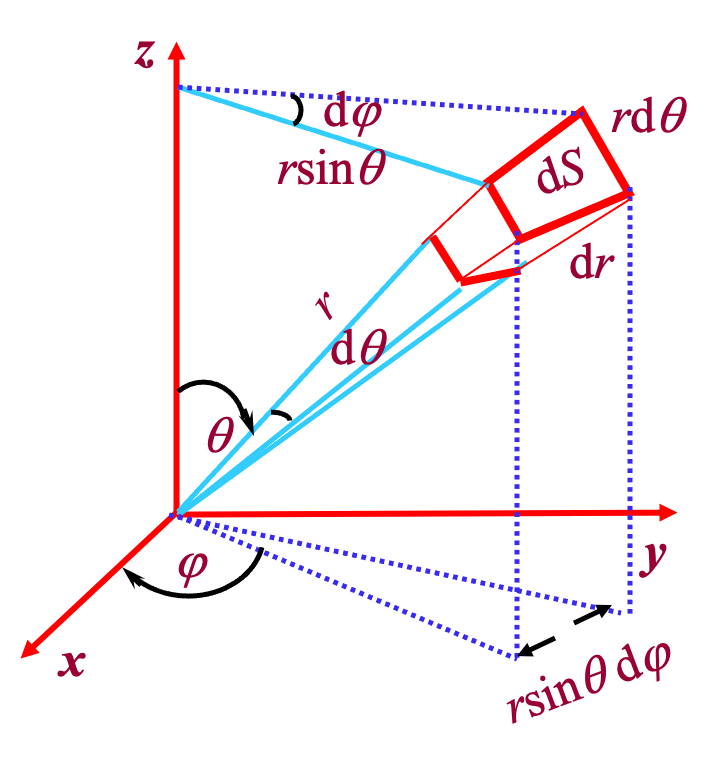
\includegraphics[width=0.4\textwidth]{figs/dt.png}
  \end{center}
$$ \begin{aligned}
  dS&=(rd\theta)\cdot (r\sin \theta d \varphi ) =r^2 \sin \theta d\theta d \varphi \\
  d \tau &=dS \cdot dr = r^2 \sin \theta dr d\theta d \varphi	  
\end{aligned}$$
\end{frame}

\begin{frame}
	* 求 $N_{nl}$ 
	\begin{equation*}
	\begin{split}
		\iiint  &\Psi(r,\theta,\varphi) d \tau =1  \\
		\iiint  &|N_{nl} R (r) Y_{lm} (\theta,\varphi)| ^2 r^2 \sin \theta dr d\theta d\varphi =1  \\
		\int_{0}^{\infty}  & N^2_{nl} R^2  (r)  r^2 dr =1   \\
		\frac{1}{\alpha ^3}	&\int_{0}^{\infty}  N^2_{nl}  R^2 (\xi)  \xi^2 d\xi =1   \\
		\frac{1}{\alpha ^3} &	\int_{0}^{\infty}  N^2_{nl}  \xi ^{2l+2}  [L_{n-l-1} ^{2l+1} (\xi)]^2 e^{-\xi}  d\xi =1   \\
		\frac{1}{\alpha ^3} &	\int_{0}^{\infty}  N^2_{nl}  \xi ^{M+1}  [L_N ^M (\xi)]^2 e^{-\xi}  d\xi =1   \\
	\end{split}		
	\end{equation*}	
\end{frame}		

\begin{frame}
	\begin{equation*}
		\frac{1}{\alpha ^3} 	  N^2_{nl}  \frac{(N+M)!}{N!} (2N+M+1) =1  	
	\end{equation*}	
	$\to$ \\
	\begin{equation*}
		N^2 _{nl}  \frac{2n [(n+1)!]^3} {\alpha^3 (n-l-1)!} =1
	\end{equation*}	
	\begin{equation*}
		N_{nl}  =\sqrt{\alpha^3 \frac{ (n-l-1)!}{2n [(n+1)!]^3}} 
	\end{equation*}	
\end{frame}		

\section{5.氢原子量子描述}

\begin{frame}
	\frametitle{小结:解氢原子}
	\tcbset{enhanced jigsaw,fonttitle=\bfseries,opacityback=0.35,colback=blue!5!white,
		frame style={left color=red!75!black,right color=red!10!yellow}}
	
\begin{tikzpicture}% draw two balls
	  \path[use as bounding box] (0,0.8) rectangle +(0.1,0.1);
	  \shadedraw [shading=ball] (0,0.3) circle (1cm);
	  %\shadedraw [ball color=yellow!20] (3,-2.2) circle (1cm);
	\end{tikzpicture}
	\begin{tcolorbox}[title=\faEnvira\hspace{1em} 第一次分离变量,
	  overlay=
	  {\begin{tcbinvclipframe}
	  \draw[red,line width=1cm] ([xshift=-2mm,yshift=2mm]frame.north west)
	  --([xshift=2mm,yshift=-2mm]frame.south east);
	  \draw[red,line width=1cm] ([xshift=-2mm,yshift=-2mm]frame.south west)
	  --([xshift=2mm,yshift=2mm]frame.north east);
	  \end{tcbinvclipframe}}]
	  {\Bullet}氢原子定态薛定谔方程:
		\begin{equation*}
			\left[-\frac{\hbar^2}{2 m_1} \nabla_1 ^2  -\frac{\hbar^2}{2 m_2} \nabla_2 ^2 +U(| \vec{r_1}-\vec{r_2} | ) \right] \Psi (\vec{r_1},\vec{r_2}) =E \Psi (\vec{r_1},\vec{r_2}) 
		\end{equation*}
	{\Bullet} 质心运动方程
	  \begin{equation*}
		-\frac{\hbar^2}{2 M} \nabla_R ^2  \psi (\vec{R}) =E_c \psi (\vec{R}) 
	\end{equation*}	
	{\Bullet} 相对运动方程
	\begin{equation*}
		\left[-\frac{\hbar^2}{2 m} \nabla ^2 +U(\vec{r}) \right] \Psi (\vec{r}) =E \Psi (\vec{r})   
	\end{equation*}
	  \end{tcolorbox}
\end{frame}

\begin{frame}
	\frametitle{}
	\tcbset{enhanced jigsaw,fonttitle=\bfseries,opacityback=0.35,colback=blue!5!white,
		frame style={left color=red!75!black,right color=red!10!yellow}}
	
\begin{tikzpicture}% draw two balls
	  \path[use as bounding box] (0,0.8) rectangle +(0.1,0.1);
	  \shadedraw [shading=ball] (0,0.3) circle (1cm);
	  %\shadedraw [ball color=yellow!20] (3,-2.2) circle (1cm);
	\end{tikzpicture}
	\begin{tcolorbox}[title=\faEnvira\hspace{1em} 第二次分离变量,
	  overlay=
	  {\begin{tcbinvclipframe}
	  \draw[red,line width=1cm] ([xshift=-2mm,yshift=2mm]frame.north west)
	  --([xshift=2mm,yshift=-2mm]frame.south east);
	  \draw[red,line width=1cm] ([xshift=-2mm,yshift=-2mm]frame.south west)
	  --([xshift=2mm,yshift=2mm]frame.north east);
	  \end{tcbinvclipframe}}]
	{\Bullet}角向方程:
	\begin{equation*}
		\left[ \frac{1}{ \sin \theta  } \frac{\partial }{\partial \theta } (\sin \theta \frac{\partial }{\partial \theta } )
		+\frac{1}{ \sin^2 \theta  } \frac{\partial^2}{\partial\varphi ^2}  +l(l+1) \right] Y=0 
	\end{equation*}
	{\Bullet}径向方程:
	\begin{equation*}
		\frac{d^2 R}{d r^2} + \frac{2}{r^2}\frac{d R }{d r}  + \frac{2 \mu} {\hbar^2}(E+ \frac{e_s ^2}{r} ) R- \frac{l(l+1)}{r^2} R=0
	\end{equation*}	
	  \end{tcolorbox}
\end{frame}

\begin{frame}
	\frametitle{}
	\tcbset{enhanced jigsaw,fonttitle=\bfseries,opacityback=0.35,colback=blue!5!white,
		frame style={left color=red!75!black,right color=red!10!yellow}}
	
\begin{tikzpicture}% draw two balls
	  \path[use as bounding box] (0,0.8) rectangle +(0.1,0.1);
	  \shadedraw [shading=ball] (0,0.3) circle (1cm);
	  %\shadedraw [ball color=yellow!20] (3,-2.2) circle (1cm);
	\end{tikzpicture}
	\begin{tcolorbox}[title=\faEnvira\hspace{1em} 第三次分离变量,
	  overlay=
	  {\begin{tcbinvclipframe}
	  \draw[red,line width=1cm] ([xshift=-2mm,yshift=2mm]frame.north west)
	  --([xshift=2mm,yshift=-2mm]frame.south east);
	  \draw[red,line width=1cm] ([xshift=-2mm,yshift=-2mm]frame.south west)
	  --([xshift=2mm,yshift=2mm]frame.north east);
	  \end{tcbinvclipframe}}]
	{\Bullet}经度方程:
	\begin{equation*}
		\frac{d^{2} \Phi}{d \varphi^{2}}+\lambda \Phi=0,(0<\varphi\le2 \pi)
	\end{equation*}	
	{\Bullet}纬度方程:
	\begin{equation*}
		\frac{1}{\sin \theta} \frac{d}{d \theta}\left(\sin \theta \frac{d \Theta}{d \theta}\right)+\left[l(l+1)-\frac{\lambda}{\sin ^{2} \theta}\right] \Theta=0,(0<\theta \le \pi)
	\end{equation*}	
	{\Bullet}径向方程:
	\begin{equation*}
		\frac{d^2 R}{d r^2} + \frac{2}{r^2}\frac{d R }{d r}  + \frac{2 \mu} {\hbar^2}(E+ \frac{e_s ^2}{r} ) R- \frac{l(l+1)}{r^2} R=0
	\end{equation*}	
	  \end{tcolorbox}
\end{frame}

\begin{frame}
	\frametitle{}
	\tcbset{enhanced jigsaw,fonttitle=\bfseries,opacityback=0.35,colback=blue!5!white,
		frame style={left color=red!75!black,right color=red!10!yellow}}
	
\begin{tikzpicture}% draw two balls
	  \path[use as bounding box] (0,0.8) rectangle +(0.1,0.1);
	  \shadedraw [shading=ball] (0,0.3) circle (1cm);
	  %\shadedraw [ball color=yellow!20] (3,-2.2) circle (1cm);
	\end{tikzpicture}
	\begin{tcolorbox}[title=\faEnvira\hspace{1em} 经度方程的解,
	  overlay=
	  {\begin{tcbinvclipframe}
	  \draw[red,line width=1cm] ([xshift=-2mm,yshift=2mm]frame.north west)
	  --([xshift=2mm,yshift=-2mm]frame.south east);
	  \draw[red,line width=1cm] ([xshift=-2mm,yshift=-2mm]frame.south west)
	  --([xshift=2mm,yshift=2mm]frame.north east);
	  \end{tcbinvclipframe}}]
	{\Bullet}经度方程:
	\begin{equation*}
		\frac{d^{2} \Phi}{d \varphi^{2}}+\lambda \Phi=0,(0<\varphi\le2 \pi)
	\end{equation*}	
	固有值和固有函数:
	\[\begin{cases}
		\lambda=m^2, ~~~ (m=0,\pm 1,\pm 2,\cdots,\pm l) \\ 
		\Phi_m (\varphi)=\frac{1}{\sqrt{2\pi}} e^{im\varphi}
	\end{cases}\]
	物理上对应角动量Z方向投影:
	\[L_z =m\hbar \]
	\end{tcolorbox}
\end{frame}

\begin{frame}
	\frametitle{}
	\tcbset{enhanced jigsaw,fonttitle=\bfseries,opacityback=0.35,colback=blue!5!white,
		frame style={left color=red!75!black,right color=red!10!yellow}}
	
\begin{tikzpicture}% draw two balls
	  \path[use as bounding box] (0,0.8) rectangle +(0.1,0.1);
	  \shadedraw [shading=ball] (0,0.3) circle (1cm);
	  %\shadedraw [ball color=yellow!20] (3,-2.2) circle (1cm);
	\end{tikzpicture}
	\begin{tcolorbox}[title=\faEnvira\hspace{1em} 纬度方程的解,
	  overlay=
	  {\begin{tcbinvclipframe}
	  \draw[red,line width=1cm] ([xshift=-2mm,yshift=2mm]frame.north west)
	  --([xshift=2mm,yshift=-2mm]frame.south east);
	  \draw[red,line width=1cm] ([xshift=-2mm,yshift=-2mm]frame.south west)
	  --([xshift=2mm,yshift=2mm]frame.north east);
	  \end{tcbinvclipframe}}]
	  {\Bullet}纬度方程:
	  \begin{equation*}
		  \frac{1}{\sin \theta} \frac{d}{d \theta}\left(\sin \theta \frac{d \Theta}{d \theta}\right)+\left[l(l+1)-\frac{m^2}{\sin ^{2} \theta}\right] \Theta=0,(0<\theta \le \pi)
	  \end{equation*}	
	固有值
	\[\begin{cases}
		 m^2, ~~~ (m=0,\pm 1,\pm 2,\cdots,\pm l) \\
		l(l+1), ~~~ (l=1, 2,\cdots, n-1) \\ 
	\end{cases}\]
	固有函数:
	\[
		\Theta_{lm}(\theta)= P^m  _{l}(\cos \theta) \]
\end{tcolorbox}
\end{frame}

\begin{frame}
	\frametitle{}
	\tcbset{enhanced jigsaw,fonttitle=\bfseries,opacityback=0.35,colback=blue!5!white,
		frame style={left color=red!75!black,right color=red!10!yellow}}
	
\begin{tikzpicture}% draw two balls
	  \path[use as bounding box] (0,0.8) rectangle +(0.1,0.1);
	  \shadedraw [shading=ball] (0,0.3) circle (1cm);
	  %\shadedraw [ball color=yellow!20] (3,-2.2) circle (1cm);
	\end{tikzpicture}
	\begin{tcolorbox}[title=\faEnvira\hspace{1em} 角向方程的解,
	  overlay=
	  {\begin{tcbinvclipframe}
	  \draw[red,line width=1cm] ([xshift=-2mm,yshift=2mm]frame.north west)
	  --([xshift=2mm,yshift=-2mm]frame.south east);
	  \draw[red,line width=1cm] ([xshift=-2mm,yshift=-2mm]frame.south west)
	  --([xshift=2mm,yshift=2mm]frame.north east);
	  \end{tcbinvclipframe}}]
	{\Bullet}角向方程:
	\begin{equation*}
		\left[ \frac{1}{ \sin \theta  } \frac{\partial }{\partial \theta } (\sin \theta \frac{\partial }{\partial \theta } )
		+\frac{1}{ \sin^2 \theta  } \frac{\partial^2}{\partial\varphi ^2}  +l(l+1) \right] Y=0 
	\end{equation*}
	角动量固有值
	\[\begin{cases}
		m\hbar, ~~~ (m=0,\pm 1,\pm 2,\cdots,\pm l) \\
		l(l+1)\hbar^2, ~~~ (l=1, 2,\cdots, n-1) \\ 
	\end{cases}\]
	固有函数:
	\[
		Y_{lm} (\theta,\varphi)= \sqrt{\frac{(2l+1)(l-m)!}{4\pi (l+m)!}}  P_l ^m (cos \theta)  e^{im\varphi}  \]
\end{tcolorbox}
\end{frame}

\begin{frame}
	\frametitle{}
	\tcbset{enhanced jigsaw,fonttitle=\bfseries,opacityback=0.35,colback=blue!5!white,
		frame style={left color=red!75!black,right color=red!10!yellow}}
	
\begin{tikzpicture}% draw two balls
	  \path[use as bounding box] (0,0.8) rectangle +(0.1,0.1);
	  \shadedraw [shading=ball] (0,0.3) circle (1cm);
	  %\shadedraw [ball color=yellow!20] (3,-2.2) circle (1cm);
	\end{tikzpicture}
	\begin{tcolorbox}[title=\faEnvira\hspace{1em} 径向方程的解,
	  overlay=
	  {\begin{tcbinvclipframe}
	  \draw[red,line width=1cm] ([xshift=-2mm,yshift=2mm]frame.north west)
	  --([xshift=2mm,yshift=-2mm]frame.south east);
	  \draw[red,line width=1cm] ([xshift=-2mm,yshift=-2mm]frame.south west)
	  --([xshift=2mm,yshift=2mm]frame.north east);
	  \end{tcbinvclipframe}}]
	  {\Bullet}径向方程:
	  \begin{equation*}
		\frac{d^2 R}{d r^2} + \frac{2}{r^2}\frac{d R }{d r}  + \frac{2 \mu} {\hbar^2}(E+ \frac{e_s ^2}{r} ) R- \frac{l(l+1)}{r^2} R=0
	  \end{equation*}	
	能量固有值
	\[ E_n =- \frac{1}{n^2} \frac{\mu e^4 _s }{2 \hbar ^2} =\frac{E_1}{n^2}, \qquad (n=1,2,3,\cdots) \]
	固有函数:
	\[
		R_{nl} (r) =\sqrt{(\frac{2}{n a_0})^3 \frac{ (n-l-1)!}{2n [(n+1)!]^3}}  (\frac{2}{n a_0}r) ^l  L_{n-l-1} ^{2l+1} (\frac{2}{n a_0}r) e^{-\frac{r}{n a_0}}\]
\end{tcolorbox}
\end{frame}


\begin{frame}
	\frametitle{}
	\tcbset{enhanced jigsaw,fonttitle=\bfseries,opacityback=0.35,colback=blue!5!white,
		frame style={left color=red!75!black,right color=red!10!yellow}}
	
\begin{tikzpicture}% draw two balls
	  \path[use as bounding box] (0,0.8) rectangle +(0.1,0.1);
	  \shadedraw [shading=ball] (0,0.3) circle (1cm);
	  %\shadedraw [ball color=yellow!20] (3,-2.2) circle (1cm);
	\end{tikzpicture}
	\begin{tcolorbox}[title=\faEnvira\hspace{1em} 氢原子的解,
	  overlay=
	  {\begin{tcbinvclipframe}
	  \draw[red,line width=1cm] ([xshift=-2mm,yshift=2mm]frame.north west)
	  --([xshift=2mm,yshift=-2mm]frame.south east);
	  \draw[red,line width=1cm] ([xshift=-2mm,yshift=-2mm]frame.south west)
	  --([xshift=2mm,yshift=2mm]frame.north east);
	  \end{tcbinvclipframe}}]
	  {\Bullet}	氢原子波函数:
	\begin{equation*}	
		 \Psi_{nlmm_s}(r, \theta, \varphi, s)= R_{nl} (r) Y_{lm} (\theta,\varphi)S_{m_s}(s)
	\end{equation*} 
	\begin{itemize}
		  \item 主量子数: $n=1,2,3,\cdots$, 能级,轨道能量 (主 K,L,M, N, O, P, Q)
		  \item 角量子数: $l=0,1,2,\cdots, n-1$, 角动量大小, 轨道形状 (次 s, p, d, f) 
		  \item 磁量子数: $m=0,\pm 1,\pm 2,\cdots, \pm l$, 角动量方向, 轨道空间取向 
		  \item 自旋量子数: $m_s=\pm 1/2$
	\end{itemize}
\end{tcolorbox}
\end{frame}


\begin{frame}
	  \frametitle{轨道波函数}
	  \begin{center}
		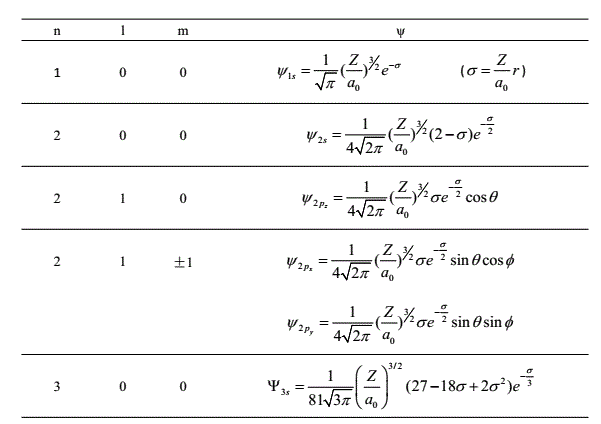
\includegraphics[width=0.95\textwidth]{figs/orbitals.png}
   \end{center}
\end{frame}

\begin{frame}
	  \frametitle{能级与光谱}
	  \[ E_n = - \frac{1}{n^2} \frac{\mu e^4 _s }{2 \hbar ^2} =\frac{E_1}{n^2}, \quad (n=1,2,3,\cdots) , \qquad \nu=\frac{E_n -E_m}{h} = R_H c [\frac{1}{m^2} -\frac{1}{n^2}]
	  \]
	  \begin{center}
		   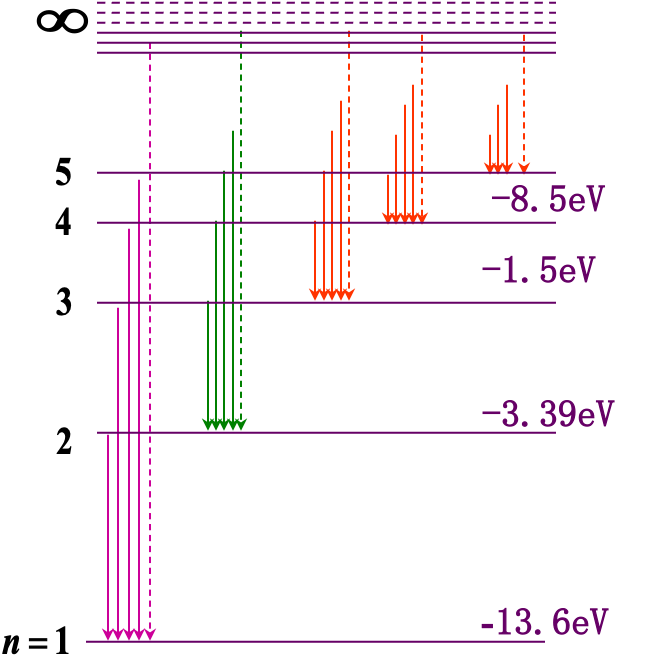
\includegraphics[width=0.40\textwidth]{figs/spectra.png}
	  \end{center}
\end{frame}

\begin{frame} 
    \frametitle{角动量量子化}
    \begin{wrapfigure} {b} {0.4\textwidth} %;图在右
        \includegraphics[width=0.35\textwidth]{figs/LandL2.png}   
    \end{wrapfigure}
    {\Bullet} 角动量大小  $L^2=l(l+1) \hbar^2$\\
	$L=\sqrt{l(l+1)}\hbar, \quad (l=1,2,\cdots, n-1)$\\
    ~~\\ \vspace{0.3em}
    {\Bullet} 角动量Z投影 $L^2_z=m^2\hbar^2$\\
    $L_z=m\hbar, \quad (m=0,\pm 1,\pm 2, \cdots, \pm l)$\\
	~~\\
    {\Bullet} 大小和方向皆量子化
\end{frame} 

\begin{frame}
	  \frametitle{轨道的形态}
		\begin{center}
			 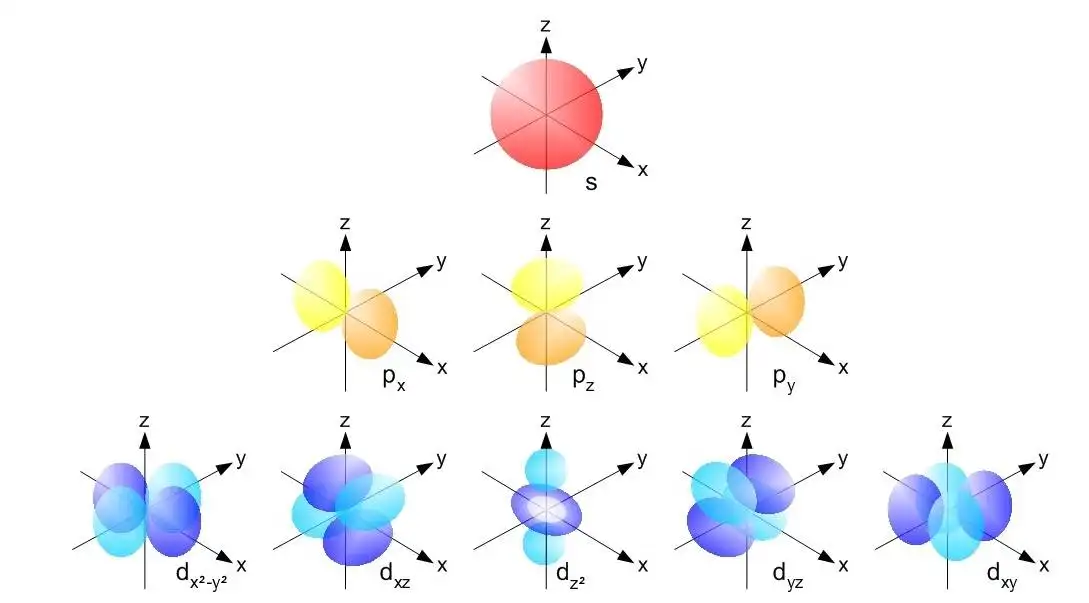
\includegraphics[width=1.0\textwidth,height=2.5in]{figs/2022-03-25-19-35-50.png}
		\end{center}	 
\end{frame}	

\begin{frame}
	  \frametitle{}
	  \例 [求电子云的形态]{}
	  \begin{enumerate}
		  \item 径向分布($r-r+dr$找到粒子的概率)
		   \[ \begin{aligned}
	    \omega_{nl} dr &= \int _{\varphi=0} ^{2\pi} \int _{\theta=0} ^{\pi} |R_{nl}(r)Y_{lm}(\theta,\varphi)|^2 r^2\sin \theta dr d\theta d \varphi \\
		&= R^2_{nl}(r) r^2 dr \\
		\end{aligned}\]
		\item 角向分布($(\theta,\varphi)-(\theta+d\theta,\varphi+d\varphi)$找到粒子的概率)		
		\[ \begin{aligned}
			\omega_{lm} d \Omega &= \int _{r=0} ^{\infty} |R_{nl}(r)Y_{lm}(\theta,\varphi)|^2 r^2dr  d \Omega \\
			&= |Y_{lm}|^2 d \Omega 	
			\end{aligned}\]		
	  \end{enumerate}  
\end{frame}
%%%%%%%%%%%%%%%%%%%%%%%%%%%%%%%%%%%%%%%%%%%%%%
\begin{frame}
	\frametitle{}
  \begin{center}
	   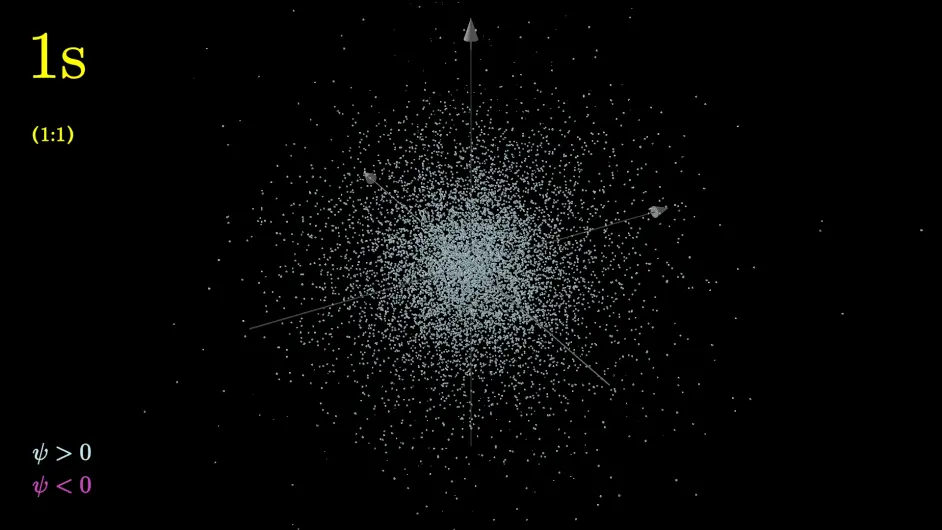
\includegraphics[width=1\textwidth]{figs/2022-03-30-18-45-45.png}
  \end{center}
\end{frame}

\begin{frame}
	\frametitle{}
  \begin{center}
	   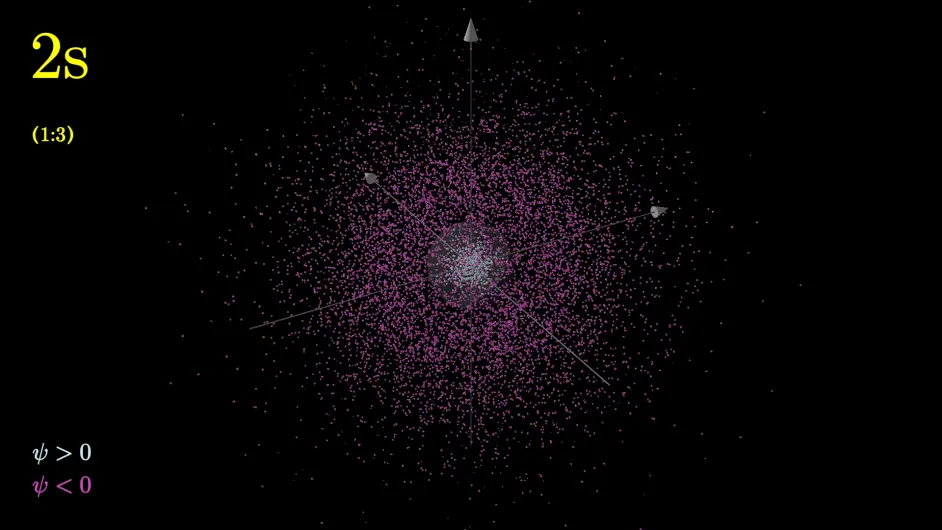
\includegraphics[width=1\textwidth]{figs/2022-03-30-18-46-37.png}
  \end{center}
\end{frame}

\begin{frame}
	\frametitle{}
  \begin{center}
	   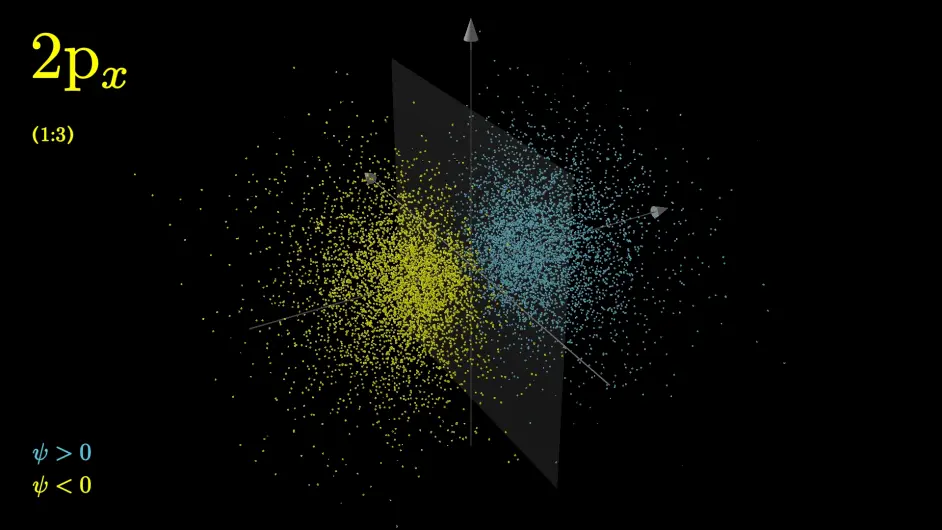
\includegraphics[width=1\textwidth]{figs/2022-03-30-18-48-34.png}
  \end{center}
\end{frame}

\begin{frame}
	\frametitle{}
  \begin{center}
	   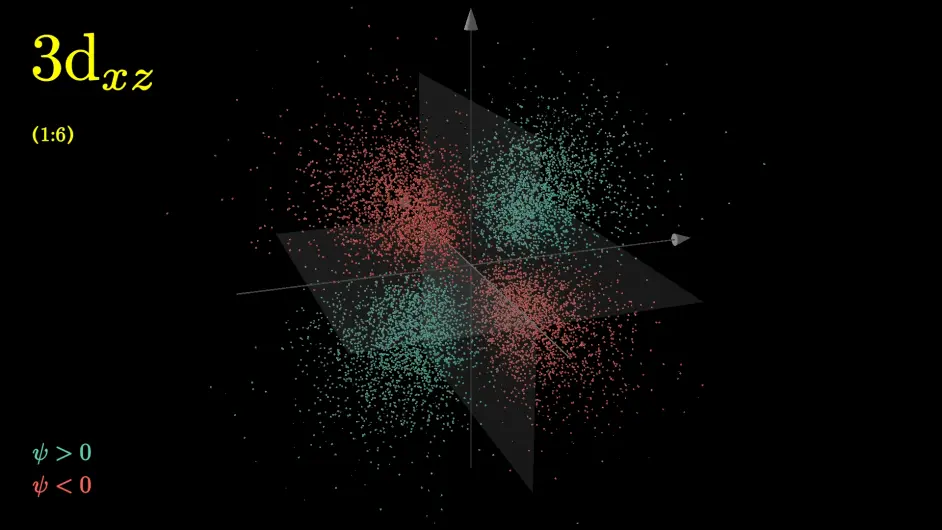
\includegraphics[width=1\textwidth]{figs/2022-03-30-18-49-45.png}
  \end{center}
\end{frame}

\begin{frame}
	\frametitle{}
  \begin{center}
	   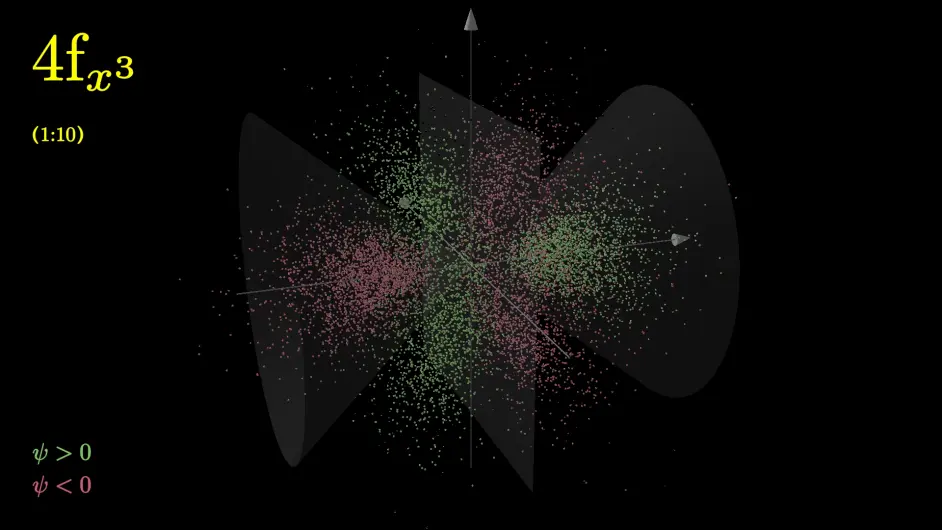
\includegraphics[width=1\textwidth]{figs/2022-03-30-18-55-10.png}
  \end{center}
\end{frame}

\begin{frame}
	\frametitle{作业}
	1、证明拉盖多项式的正交性\\
	2、求方程的解
	\begin{equation*}
		\frac{d^2 U}{d \xi ^2} + \frac{2}{\xi }\frac{d U }{d \xi}  +[\frac{\beta}{\xi} - \frac{l(l+1)}{\xi ^2}] U=0
	\end{equation*}	 
	3、计算积分:
	\begin{equation*}
		\int_{0}^{\infty}   e^{-x} ( L_1 (x) )^2 dx, \qquad  \int_{0}^{\infty}   e^{-x} ( L_2 (x) )^2 dx, 
	\end{equation*}	
	4、写出 $L_1 (x)$ 和 $L_1 ^0 (x)$ 之间的关系式
\end{frame}		

\begin{frame}
	\frametitle{随堂测试}
	\begin{exampleblock} {1.粒子处于如下势场中:}
		\begin{equation*}
			V(x)= \frac{1}{2} \mu \omega ^2 x^2  +1
		\end{equation*}
		\hspace{2em}求能量固有值和定态波函数。
	\end{exampleblock}	
	\begin{exampleblock} {2.基于厄米多项式的正交性求积分:}
		\begin{equation*}
			\int\limits_{-\infty}^{+\infty} (x^3 +1)e^{-x^{2}} H_n(x) d x 
		\end{equation*}
	\end{exampleblock}	
\end{frame}


\begin{frame}
	\frametitle{}
	\begin{exampleblock} {1.粒子处于如下势场中:}
	  \begin{equation*}
		  V(x)= \frac{1}{2} \mu \omega ^2 x^2  +1
	  \end{equation*}
	\end{exampleblock}
	  \hspace{2em}求能量固有值和定态波函数。\\	
	  \解 ~ (1)含时分离变量, 得时间函数: $T(t)  = \exp(-i E t /\hbar) $ \\
	  (2) 定态薛定谔方程:
	  \begin{equation*}
		  \begin{split}
			  \left [ -\frac{\hbar^2}{2\mu} \frac{\mathrm{d} ^2}{\mathrm{d} x^2} +\frac{1}{2}\mu \omega^2 x^2 +1 \right ]\Psi(x)&=E\Psi(x) \\ 
			  \left [ -\frac{\hbar^2}{2\mu} \frac{\mathrm{d} ^2}{\mathrm{d} x^2} +\frac{1}{2}\mu \omega^2 x^2  \right ]\Psi(x)&=(E-1)\Psi(x) 	
		  \end{split}
	  \end{equation*}
	  令 $E'=E-1$, 得:
	  \[\left [ -\frac{\hbar^2}{2\mu} \frac{\mathrm{d} ^2}{\mathrm{d} x^2} +\frac{1}{2}\mu \omega^2 x^2  \right ]\Psi(x)=E'\Psi(x) \]
	  此方程就是谐振子标准方程!
\end{frame}

\begin{frame}
		\frametitle{}	  
	  能量固有值(能级$E_n$)
	  \begin{equation*}
		  E'_n=\left(n+\frac{1}{2}\right) \hbar \omega=E_n-1, ~~~  ( n=0,1,2, ...)  
	  \end{equation*}  
	  定态波函数为
	  \begin{equation*}
		  \Psi_n(x,t) = \left( \frac{\alpha}{\sqrt{\pi} 2^n n!}  \right) ^{1/2}  \exp(-\frac{ \alpha^2 x^2}{2} -\frac{i}{\hbar} E_n t ) H( \alpha x) , \qquad (\alpha ^2= \frac{\mu\omega}{\hbar}) 
	  \end{equation*}  
\end{frame}       
%%%%%%%%%%%%%%%%%%%%%%%%%%%%%%%%%%%%55%%
\begin{frame} [plain]
    \frametitle{}
    \Background[1] 
    \begin{center}
    { {\huge 第一章:绪论 }}
    \end{center}  
    \addtocounter{framenumber}{-1}   
\end{frame}
%%%%%%%%%%%%%%%%%%%%%%%%%%%%%%%%%%
\section{1.课程简介}

\begin{frame}[t]
    \frametitle{课程目标}
        \begin{enumerate}
            \Item Learn the formal theory of Quantum Mechanics
            \IItem How physical systems are described in Quantum Mechanics.
            \Item How to solve problems in Quantum Mechanics.
        \end{enumerate}
\end{frame}
\begin{frame} [t]
    \frametitle{分数构成}
        \begin{enumerate}
            \Item Normal results 20\%
            \Item Midterm examination results 20\%
            \Item Final examination results 60\%
        \end{enumerate}
\end{frame}

\begin{frame} [t]
    \frametitle{教学效果}
    \centering
    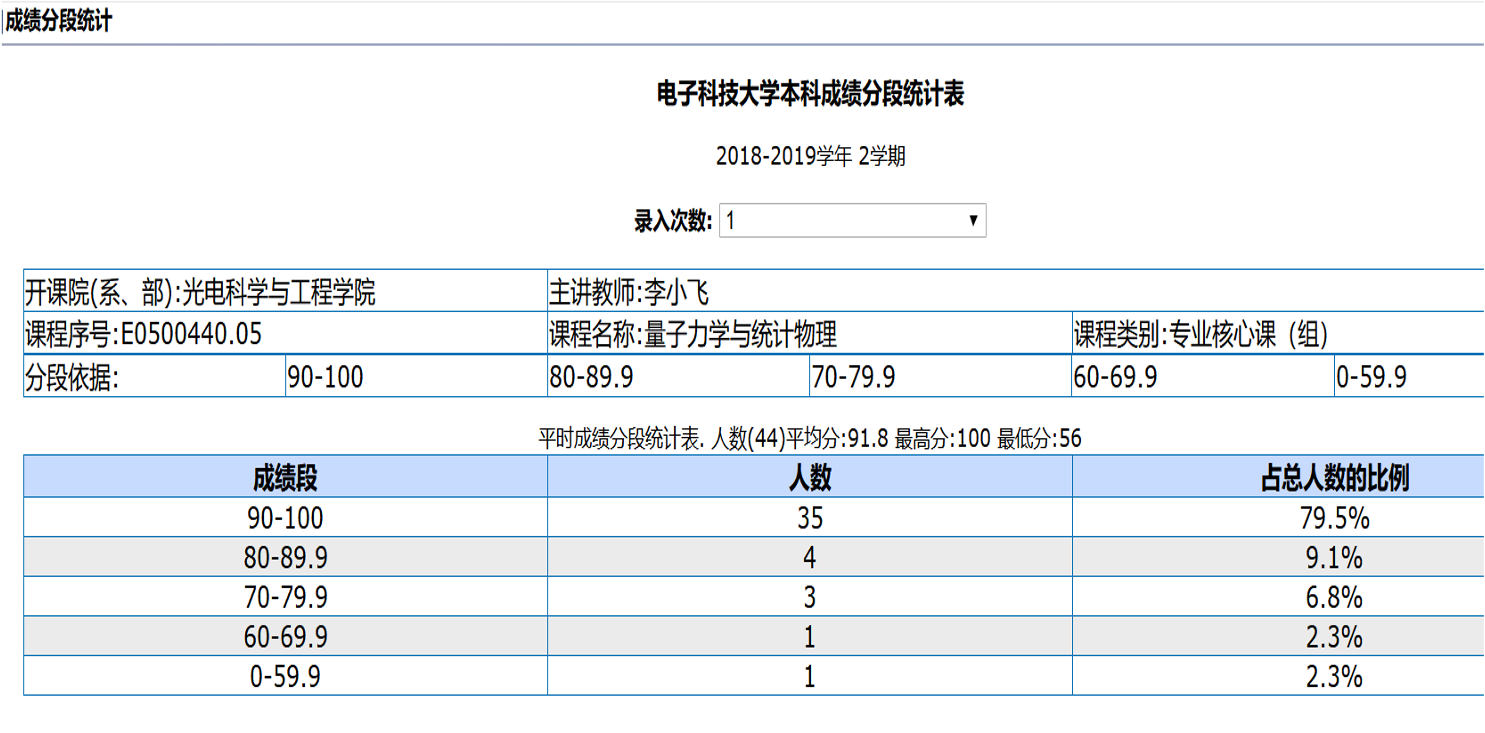
\includegraphics[width=1.0\textwidth,height=5.0cm]{figs/exam1.png}
\end{frame}

\begin{frame}[t]
    \frametitle{参考书目}
        \begin{itemize}
            \Item 《量子力学》卷I,II, 曾谨言, 科学出版社, 2008           
            \Item Principles of quantum mechanics, shankar
            \Item Modern quantum mechanics, shankar
            \Item Lectures on quantum mechanics, weinberg
            \Item Principles of quantum mechanics, Dirac
        \end{itemize}
\end{frame}

\begin{frame}[t]
    \begin{tcolorbox4}[三条军规]    
        \begin{enumerate}
            \Item Objects are wave-particles and can be in states of superposition
            \Item Rule 1 holds as long as you don't measure
            \Item Measurement gives random results
        \end{enumerate}
    \end{tcolorbox4} 
\end{frame}

\section{2.能量子假说}

\subsection{伟大成就}

\begin{frame}[t]
    \frametitle{经典物理伟大成就}
    \begin{tcolorbox3}
    [Great successes in Classical Physics]
        \begin{enumerate}
            \Item Newtonian mechanics
            \Item Maxwell's electromagnetism
            \Item Thermodynamic laws
        \end{enumerate}
    \end{tcolorbox3}  
    \begin{quotation}
        "There is nothing new to be discovered in physics now. All that remains is 
        more and more precise measurements"   \\
        \rightline{$\cdots$ Lord Kelvin (1900)\hspace{3em}}
    \end{quotation}
\end{frame}

\begin{frame}
    \frametitle{}
    \begin{quotation}
        "But the beauty and clearness ... is obscured by two small puzzling clouds \faCloud "  \\
        \rightline{$\cdots$ Lord Kelvin (1900.4)\hspace{3em}}   
    \end{quotation}
    ~~ \vspace{0.3em}
    \begin{tcolorbox4}[两朵乌云]    
        \begin{enumerate}
        \Item Michelson-Morley experiment
        \Item Black body radiation
        \end{enumerate}
    \end{tcolorbox4} 
\end{frame}

\begin{frame}
    \frametitle{迈克尔逊-莫雷实验}
    \begin{center}
    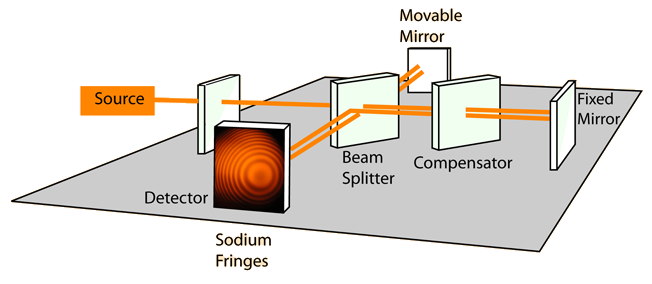
\includegraphics[width=0.8\textwidth]{figs/michel.png}
    \end{center}
There is no displacement of the interference bands. \dots 
the Stationary Ether is thus shown to be incorrect
\end{frame}

\begin{frame}
    The theory of relativity is established 
    \begin{center}
        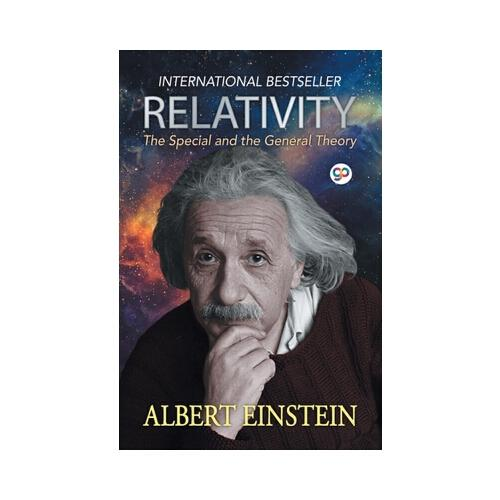
\includegraphics[width=0.4\textwidth]{figs/relativity.jpg}
    \end{center}   
    Greatly changed our view of time and space. Mainly useful in two aspects: high-speed motion, and strong gravitational field. 
\end{frame}

\begin{frame}
    \frametitle{黑体辐射实验}
    \begin{center}
    \includegraphics[width=0.7\textwidth]{figs/2021-12-01-23-47-27.png}
    \end{center}
    No mathematical function to describe the curves exactly 
\end{frame}
\begin{frame}
    Quantum mechanics is established  
    \begin{center}
        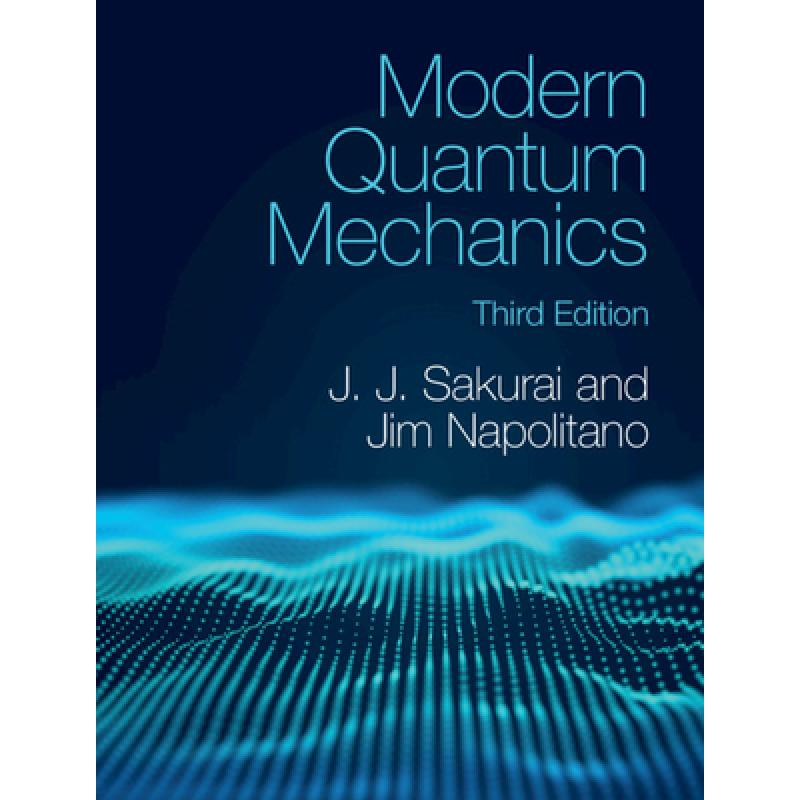
\includegraphics[width=0.45\textwidth]{figs/mqm.jpg}
    \end{center}   
    It is a theory about matter.
\end{frame}

\begin{frame}
    \frametitle{现代科学基石}
    \begin{center}
        \includegraphics[width=0.75\textwidth]{figs/stone.png}
    \end{center}   
\end{frame}

%%%%%%%%%%%%%%%%%%%%%%%%%%%%%%%%%%%%
\subsection{普朗克公式}
%%%%%%%%%%%%%%%%%%%%%%%%%%%%%%%%%%%%

\begin{frame}
    \frametitle{Black body radiation}
    \begin{definition}[Black body: ]
    \hspace{2em}absorb all electromagnetic waves in any temperature
    \end{definition}
    \begin{center}
        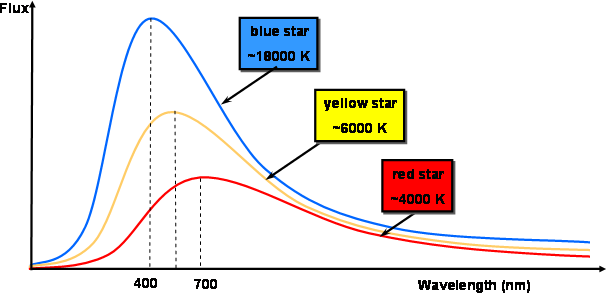
\includegraphics[width=0.55\textwidth]{figs/blackbody_radn_curves.png}
    \end{center}
    \textbf{\color{deepred} Most interestingly}, what is the mathematical function that describes all of these curves?
\end{frame}

\begin{frame}
    \frametitle{三个经验公式}
    \begin{center}
        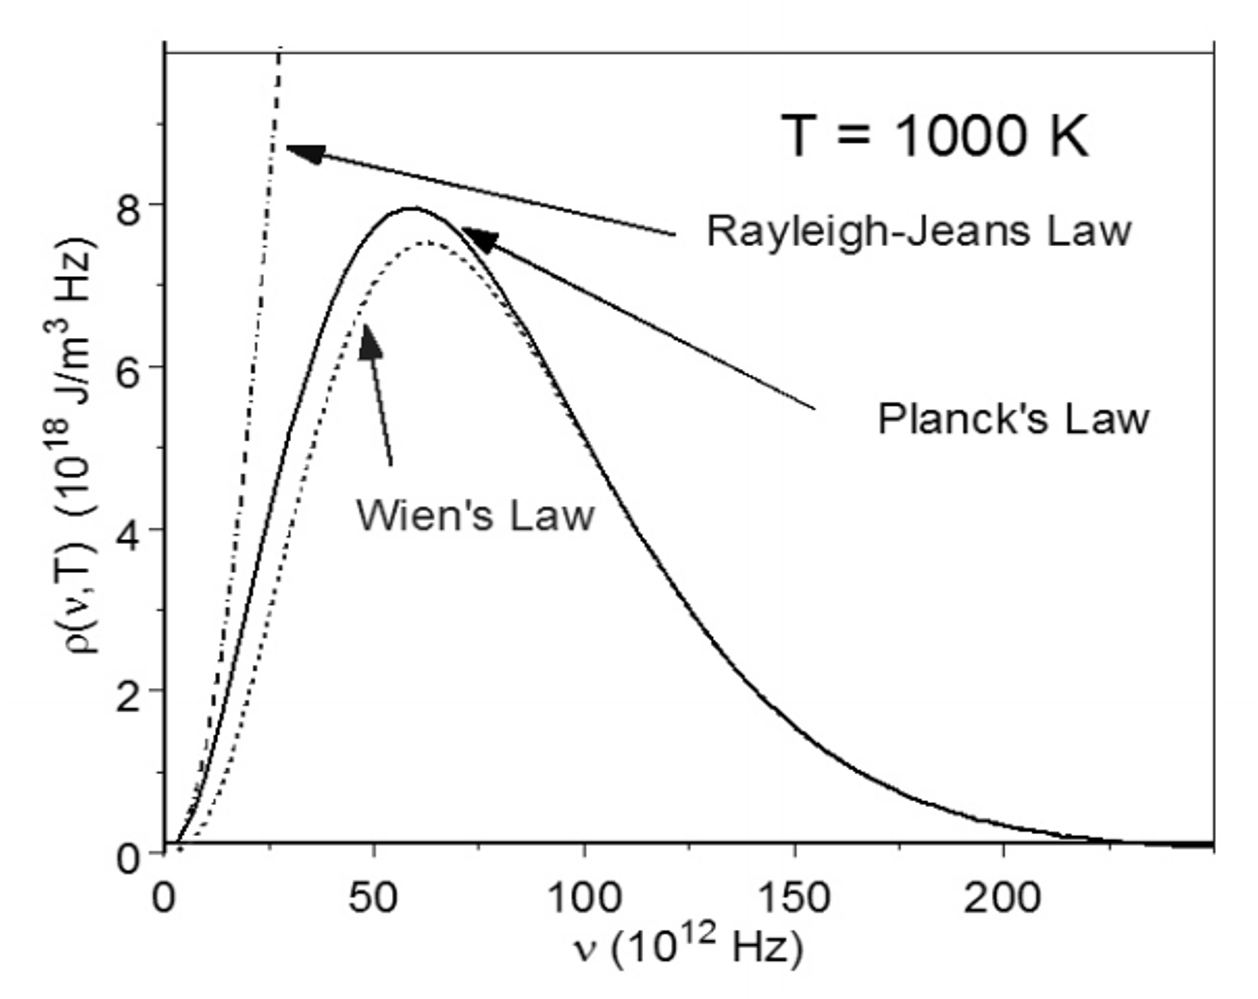
\includegraphics[width=0.7\textwidth]{figs/threelaws.png}
    \end{center}
\end{frame}

\begin{frame} [t]
    \frametitle{维恩公式}
    \begin{equation*}
        \rho(\nu) d \nu=c_{1} \nu^{3} e^{-c_{2} \nu / T} d \nu 
    \end{equation*}
    Derived from electromagnetism (1893), but described well only in high frequency region.\\ 
    {\color{deepred} Nobel Prize in physics(1911)}\\
\end{frame}

\begin{frame}[t]
    \frametitle{瑞-金公式}
    \begin{equation*}
        \rho(\nu, T) d \nu=\frac{8 \pi}{c^{3}} \nu^{2} k T d \nu 
    \end{equation*}
    Derived from thermodynamics (1900), but described well only in low frequency region.\\ 
   {\color{deepred} Nobel Prize in physics(1904)}\\ \vspace{0.3em}
   {\color{deepblue} {\Bullet} Ultraviolet Catastrophe:} 
    \begin{equation*}
         \int_0 ^\infty \frac{8 \pi}{c^{3}} \nu^{2} k T d \nu \to \infty 
    \end{equation*}
\end{frame}

\begin{frame}
    \frametitle{普朗克公式}
    On 1900-10-19, at the German Physical Society, 
    Max Planck presented a resolution to {\color{deepblue} Ultraviolet Catastrophe} 
    \begin{equation}
        \boxed{\rho(\nu, T) d \nu=\frac{8 \pi}{c^{3}} \frac{h \nu^{3}}{e^{h \nu / K T}-1} d \nu}
    \end{equation}
    Obtained from experimental data via interpolation technique, described well in whole region \\
    {\color{deepred} Nobel Prize in physics(1918)}\\
\end{frame}

\begin{frame}
    \centering
    \begin{tcbb}[0.7]{Problems}{
        How to derive the formula from existing theory.}
    \end{tcbb}
\end{frame}

\begin{frame}
    \begin{tcolorbox2}{Solution}
        On 1900-12-14, Planck gives out his solution based on the Energy Quantum Hypothesis  
    \end{tcolorbox2}
\end{frame}

%%%%%%%%%%%%%%%%%%%%%%%%%%%%%%%%%%%%
\subsection{能量子假说}
%%%%%%%%%%%%%%%%%%%%%%%%%%%%%%%%%%%%
\begin{frame}{能量子假说}
    \begin{tcolorbox4}[Energy quantum hypothesis]
    Assuming the oscillators of the cavity could only radiate at a discrete amounts of energy
    \begin{equation}
        E=n\varepsilon
    \end{equation}
    where, the $\varepsilon$ is the unit of the energy (quanta) determined by the oscillator' frequency 
    \begin{equation}
        \varepsilon=h\nu
    \end{equation}
    and the $h=6.6260693(11)\times10^{-34} J\cdot s $ is the Planck constant. 
    \end{tcolorbox4}
\end{frame}

\begin{frame} {推导公式}
    Based on Boltzmann distribution law,
    \begin{equation*}
        \frac{N_{i}}{N}=\frac{\exp \left(-\frac{E_{i}}{k T}\right)}{\sum_{i} \exp \left(\frac{-E_{i}}{k T}\right)}
    \end{equation*}
    {\Bullet} when the energy is continuous,the distribution between $E - dE$ should be 
    \begin{equation*}
        \frac{e^{-E / k T}}{\int\limits_{0}^{\infty} e^{-E / k T} d E}
    \end{equation*}  
    the average energy 
    \begin{equation*}
        <E>=\int\limits_{0}^{\infty} E \frac{e^{-E / k T}}{\int\limits_{0}^{\infty} e^{-E / k T} d E} d E
    \end{equation*}
\end{frame}

\begin{frame}
    \begin{equation*}
        \begin{split}
            <E> &= -kT \frac{Ee^{-E / k T}\vert_0 ^\infty-\int\limits_{0}^{\infty} e^{-E / k T} d E } {\int\limits_{0}^{\infty} e^{-E / k T} d E }\\  
                &= kT
        \end{split}  
    \end{equation*} 
    {\Bullet} when the energy is discrete,the distribution should be   
    \begin{equation*}
        \frac{e^{-E / k T}}{\int\limits_{0}^{\infty} e^{-E / k T} d E} 
        \to \frac{e^{-E / k T}}{\sum\limits_{0}^{\infty} e^{-E / k T}} 
        \to \frac{e^{-nh\nu / k T}}{\sum\limits_{0}^{\infty} e^{-nhv / k T}} 
    \end{equation*}    
\end{frame}

\begin{frame}
    the average energy 
    \begin{equation*}
        \begin{split}
            <E> &= \sum\limits_{0}^{\infty} nh\nu\frac{e^{-nh\nu / k T}}{\sum\limits_{0}^{\infty} e^{-nh\nu / k T}} \\
            &= -h\nu \frac{d}{dx} \frac{n e^{-nx}}{\sum\limits_{0}^{\infty} e^{-nx}} \\
            &= \frac{h\nu}{e^{h\nu/kT}-1} 
        \end{split} 
    \end{equation*}
    We get
    \begin{equation*}
        \text{(continuous)} \quad k T \rightarrow \frac{h \nu}{e^{ h \nu / k T}-1} \quad \text{(discrete)} 
    \end{equation*}
\end{frame}

\begin{frame}
    In Rayleigh-Jeans formula
    \begin{equation*}
        \rho(\nu, T) d \nu=\frac{8 \pi}{c^{3}} \nu^{2} k T d \nu 
    \end{equation*}
    the item $kT$ should be replaced by $\dfrac{h \nu}{e^{ h \nu / k T}-1}$
    \begin{equation*}
        \rho(\nu, T) d \nu=\frac{8 \pi}{c^{3}} \frac{h \nu^{3}}{e^{h \nu / K T}-1} d \nu
    \end{equation*}
    It is the Planck's formula exactly 
\end{frame}

\begin{frame}
    \begin{tcolorbox4}[Revolutionary Significance]
        Planck's Energy Quantum Hypothesis broke through the constraints of classical physics and 
        opened the door of quantum mechanics 
    \end{tcolorbox4}
\end{frame}

\begin{frame}
    \frametitle{}
    \centering
    \tcbb[0.68]{一只会下金蛋的鹅}
    {
    历史上,普朗克,德拜,艾伦菲斯特,劳厄,洛伦兹,庞加莱,泡利,玻色,爱因斯坦等从多角度推导过普朗克公式,每一次推导都给物理学带来了新的知识内容 
    }

 《黑体辐射公式的多种推导及其在近代物理构建中的意义》- 返朴|曹则贤
\end{frame}

%\begin{frame}
%    \begin{tcolorbox}[colback=yellow!10,colframe=red!75!black,title=THE END]
%    In 1927, Dirac got the Planck's formula from Quantum Mechanism.  
%    \end{tcolorbox}
%\end{frame}

\begin{frame}
    \frametitle{}
    \begin{tcolorbox3}[学术讨论]
        普朗克黑体辐射公式重要,还是能量量子化观念重要?\\
        能量量子化只是一种数学处理工具?
    \end{tcolorbox3}
\end{frame}

%\begin{frame}
%    \frametitle{Homework}
%    \begin{enumerate}
%        \item Planck's Energy Quantum Hypothesis
%        \item What's the quanta
%        \item Deriving the Rayleigh-Jeans formula and Wien's formula from Planck's formula
%    \end{enumerate}
%\end{frame}
%%%%%%%%%%%%%%%%%%%%%%%%%%%%%%%%%%%%%%%%%%%%%%%%%%%%%%%%%%%%%%%%%%%
%\section{3.波粒二象性}      

\begin{frame}
    \frametitle{}
    \begin{tcolorbox3}[前情回顾]
        Assuming the oscillators can radiate at a discrete amounts of energy
        \[    E=n\varepsilon, \qquad (n=1,2,3,\cdots) \]
        and the unit of the energy is determined by the oscillator' frequency
        \[   \varepsilon=h\nu  \]
        one can derive the framula:
        \[ \rho(\nu, T) d \nu=\frac{8 \pi}{c^{3}} \frac{h \nu^{3} }{e^{h \nu / K T}-1} d \nu \]
    \end{tcolorbox3}
\end{frame}

\begin{frame}
    \frametitle{粒-波的不可调和性}
	\begin{columns}
		\begin{column}[t]{0.46\linewidth}
			粒子性
			\begin{itemize}
				\Item  确定的位置、能量、动量等
				\Item  两个粒子不能同时占据同一位置
				\Item  同一粒子也不能同时占据多个位置
				\Item  碰撞现象
			\end{itemize}
		\end{column}
		\begin{column}[t]{0.46\linewidth}
			波动性
			\vspace{1ex}
			\begin{itemize}
				\Item  确定的波长、振幅、相位等
				\Item  可以同时出现在同一位置
				\Item  可以同时占据多个位置
				\Item  衍射、干涉,无碰撞
			\end{itemize}
		\end{column}
	\end{columns}
\end{frame}

\begin{frame} 
    人们通过上述特性进行判定\\
    \begin{itemize}
        \Item  一个物体要么是粒子,要么是波
        \Item  这个方法一直是有效
        \Item  直到遇到**光** 
    \end{itemize}   
    \begin{figure}
        \centering
        \subfigure[]{\includegraphics[width=7.4cm]{figs/2021-12-02-15-26-40.png}}
        \subfigure[]{
\includegraphics[width=4.5cm]{figs/2021-12-06-11-44-50.png}}
        %\caption{} %图片标题
        %\label{fig:1}  
    \end{figure} 
    \setcounter{subfigure}{0}
\end{frame}

\begin{frame}
	\begin{columns}
		\begin{column}[t]{0.46\linewidth}
            水波
            \begin{center}
                \includegraphics[width=2.5in,height=2.5in]{figs/2021-12-02-15-46-16.png}
            \end{center}
		\end{column}
		\begin{column}[t]{0.46\linewidth}
            光波
            \begin{center}
                \includegraphics[width=2.5in,height=2.5in]{figs/2021-12-02-15-49-36.png}
            \end{center}
		\end{column}
	\end{columns}
\end{frame}

\begin{frame} {光的波动说}
    \begin{center}
        \includegraphics[width=0.70\textwidth]{figs/2021-12-02-16-23-16.png}
    \end{center}
    光只是一定波长范围内的电磁波
\end{frame}

\begin{frame} 
    波动说面临的困难:
    \begin{itemize}
        \Item  黑体辐射
        \Item  光电效应
        \Item  康普顿效应
        \Item  氢原子光谱
    \end{itemize}
\end{frame}

%%%%%%%%%%%%%%%%%%%%%%%%%%%%%%%%%%%%
\subsection{光电效应}
%%%%%%%%%%%%%%%%%%%%%%%%%%%%%%%%%%%%

\begin{frame} 
    \frametitle{光电效应实验}   
    \begin{center}
       \includegraphics[width=0.53\textwidth]{figs/2021-12-02-16-01-21.png}
   \end{center}  
   \bullet 具有瞬时性 \\
   \bullet 存在临界频率 $\nu_0$ \\
   \bullet 光电子能量由光的频率决定
\end{frame}  

\begin{frame} 
    In 1905, Einstein considered the derivation of Planck's Law  \\
    \begin{itemize}
        \Item  Plank’s Law was consistent with experment but not with existing theory
        \Item  Rayleigh-Jeans Law was consistent with existing theory but not with experiment
        \Item  For treating Ultraviolet Catastrophe, he proposed the light quantum hypothesis
        \Item  Using light quantum hypothesis, he explained the Photoelectric effect
    \end{itemize}
\end{frame}

\begin{frame}
    \frametitle{}
        \begin{figure}
            \centering
            \subfigure[光强分布]{\includegraphics[width=0.495\textwidth]{figs/blackbody_radn_curves.png}}
            \subfigure[粒子数分布]{\includegraphics[width=0.495\textwidth]{figs/2022-01-17-14-21-43.png}}
        \end{figure}
    \setcounter{subfigure}{0}
\end{frame}

\begin{frame} 
    \begin{tcolorbox4}[Light quantum hypothesis]
        \bullet Light likes particles with unit energy  (quanta).\\
        \[E=h\nu\]  
        \bullet The energy of n light quantum is $nh\nu$. \\
        \bullet The momentum of light quantum is (1918) \\
        \[p=\frac{E}{c}=\frac{h\nu}{c}=\frac{h}{\lambda}\]
    \end{tcolorbox4}
\end{frame}

\begin{frame} 
    基于光量子假说,提出光电效应公式
    \[
    \frac{1}{2}m_eV_0^2=h\nu-W
    \]
    \begin{itemize}
        \Item  瞬时性:光子碰上电子时,能量被瞬时吸收
        \Item  临界频率:$\nu_0=\frac{W}{h} $
        \Item  光电子能量与光的频率决定: $E_k=h\nu-W$
    \end{itemize}
    {\color{deepred} Nobel Prize in physics(1921)}
\end{frame}

\begin{frame} 
    基于光电效应公式:
$$
\frac{1}{2}m_eV_0^2=h\nu-W
$$
1916年,密立根实验上测定普朗克系数,验证光子说\\
\color{deepred}{1923年诺贝尔物理学奖} 
\end{frame}

\begin{frame} 
    \begin{tcolorbox4}[光量子假说的意义]
        \begin{itemize}
            \Item  揭示能量子的本质:在于光本身是量子化的,具有粒子性
            \Item  揭示光的本质:光既具波动性又具粒子性。
        \end{itemize}
    \end{tcolorbox4}
    \begin{quotation}
        "在近代物理学结出硕果的那些重大问题中,很难找到一个问题是爱因斯坦没有做出过重要贡献的。
        在他的各种推测中,他有时可能也曾经没有中标的,例如他的光量子假设,就有点迷失了方向\dots"  \\
        \rightline{$\cdots$ 普朗克\hspace{3em}}   
    \end{quotation}
\end{frame}

%%%%%%%%%%%%%%%%%%%%%%%%%%%
\subsection{康普顿效应}
%%%%%%%%%%%%%%%%%%%%%%%%%%%

\begin{frame}   
    \frametitle{康普顿效应 (1922)}
    \begin{center}
        \includegraphics[width=0.8\textwidth]{figs/compton.png}
    \end{center}  
    经验公式:$\lambda_{out}-\lambda_{in}=\lambda_e(1-\cos \theta)$
\end{frame}

\begin{frame}  
    推导经验公式\\
    \alert{解:} Energy of electron 
    \begin{equation*}
        E^2 =m_ec^2=p^2c^2 +m_0 ^2 c^4 
    \end{equation*}
    Energy of light quantum
    \begin{equation*}
        E =pc 
    \end{equation*}
    energy conservation law
    \begin{equation*}
        \begin{split}
        E_i + m_0 c^2 &= E_o + m_ec^2 \\
        (E_i -E_o + m_0 c^2)^2 &= E_e ^2\\
        (p_i c-p_o c + m_0 c^2) ^2 &= p_e ^2 c^2 +m_0 ^2 c^4 \\
        (p_i-p_o)^2 +2 m_0 (p_i c-p_o c) &= p_e ^2
    \end{split}
    \end{equation*}
\end{frame}

\begin{frame}  
    momentum conservation law
    \begin{equation*}
        \begin{split}
            \vec{p}_i -\vec{p}_o &= \vec{p}_e \\
            (\vec{p}_i -\vec{p}_o)\cdot (\vec{p}_i -\vec{p}_o)  &= \vec{p}_e\cdot \vec{p}_e   \\
            p_i ^2 + p_o ^2 -2p_i p_o \cos \theta &= p_e ^2  \\
            p_i ^2 + p_o ^2 -2p_i p_o \cos \theta &= (p_i-p_o)^2 +2 m_0 (p_i c-p_o c) \\
            \frac{1}{p_o} -\frac{1}{p_i} &= \frac{1}{m_0 c} (1-\cos \theta) \\
            \lambda_o -\lambda_i &= \frac{h}{m_0 c} (1-\cos \theta) 
        \end{split}
    \end{equation*}
\end{frame}

\begin{frame}   
    \begin{tcolorbox3}[Significance]
        Prove that:\\
        \bullet The light of wavelength ($\lambda$) possesses a quantum momentum \[p=\frac{h}{\lambda}\]
        \bullet Momentum conservation law works in subatom scales 
    \end{tcolorbox3}   
    \color{deepred}{Nobel Prize in physics(1927)}\\
\end{frame}

%%%%%%%%%%%%%%%%%%%%%%%%%%
\subsection{氢原子光谱}
%%%%%%%%%%%%%%%%%%%%%%%%%%

\begin{frame}  
     \frametitle{氢原子光谱}
     \begin{center}
        \includegraphics[width=0.6\textwidth]{figs/2022-01-17-14-02-45.png}
    \end{center}  
    经验公式:
       $\dfrac{1}{\lambda}=R_H c (\dfrac{1}{m^2} -\dfrac{1}{n^2})$ \\ \vspace{0.3em}
    \alert{Problem:} the formula cannot be derived from existing theory
\end{frame}

\begin{frame} 
    \frametitle{Rutherford model}  
    \begin{center}
        \includegraphics[width=0.8\textwidth]{figs/utherford_atom.png}
    \end{center}  
\end{frame}

\begin{frame}  
    \begin{tcolorbox4}[Bohr's hydrogen atom hypothesis]
    Bohr asummed that :\\
    \bullet Stationary states: Electrons move around the nucleus only in certain allowed circular orbits with fixed energy \\
    \[ L=n \frac{h}{2\pi}= n \hbar,\qquad (\oint p_i dq_i = n_i h)\]
    \bullet Quantum transition: Electron can jump between stationary state orbits when absorbed or emitted a photon with certain energy\\
    \[ h\nu=E_n -E_m \]
    \end{tcolorbox4}
\end{frame}

\begin{frame}   
    \frametitle{}
    推导光谱公式\\
    \bullet Stationary state orbit radius:
    \begin{equation*}
        \begin{split}
            m\frac{v^2}{r}&=\frac{1}{4\pi\epsilon_0} \frac{e^2}{r^2} \\
            L=&mvr =n\hbar \\
            r_n&= n^2 (\frac{\epsilon_0 h^2}{m\pi e^2}) =n^2 r_1   
        \end{split} 
     \end{equation*}
     \bullet Stationary state orbit energy: 
     \begin{equation*}
        \begin{split}
            E_n &= T + U \\
            &= \frac{1}{2}mv^2- \frac{1}{4\pi\epsilon_0} \frac{e^2}{r_n ^2} \\
            &= \frac{1}{n^2} (-\frac{m e^4}{8 \epsilon_0 ^2 h^2}) = \frac{E_1}{n^2}
        \end{split}  
     \end{equation*}
\end{frame}

\begin{frame}
    \bullet Spectrum formula: 
    \begin{equation*}
        \begin{split}
         \nu&=\frac{E_n -E_m}{h} \\
         &= \frac{m e^4}{4\pi \hbar ^3} [\frac{1}{m^2} -\frac{1}{n^2}]
        \end{split}  
     \end{equation*}
     \bullet Rydberg constant : 
     \[R_{theo}= \frac{m e^4}{4\pi \hbar ^3 c} =1.0973731\times 10^7 m^{-1}\]
    \[R_{exp}=1.0974\times10^7 m^{-1} \]  
\end{frame}

\begin{frame}   
    \frametitle{Bohr's model}  
    \begin{center}
        \includegraphics[width=0.6\textwidth]{figs/bohratom.png}
    \end{center}  
    \bullet 1905年爱因斯坦提出的光子概念,不受名人的重视,普朗克把爱因斯坦的光量子概念说成是“迷失了方向”。\\
    \bullet 1913年,28岁的玻尔,创造性地把光子概念用到卢瑟福模型上,成功破解氢原子光谱问题 \\
    {\color{deepred} \bullet Nobel Prize in physics(1922)}\\ 
\end{frame}

\subsection{光的波粒二象性} 

\begin{frame} 
  \frametitle{光的波粒二象性}  
  \bullet In 1905, when Einstein first put forward this hypothesis, 
  he simply stated that light consisted of quanta with energy \[ E = h\nu \] 
  \bullet In 1917, he stated that the light quantum carried a momentum of  \[ p=\frac{h}{\lambda}\]
  At this point, the light quantum with massless particle property was named as photon (光子)
\end{frame}

\begin{frame}  
  $\begin{cases}
    \text{Light behaves like waves }\\
    \text{~~\qquad Interference} \\
    \text{~~\qquad Diffraction} \\
    \text{Light behaves like particles}\\
    \text{~~\qquad Black body radiation} \\
    \text{~~\qquad Photoelectric effect} \\
    \text{~~\qquad Compton effect} \\
   \end{cases}$\\
   ~~\\
   Light has both wave and particle properties is called \alert{wave-particle duality} of light
\end{frame}

\begin{frame}
    \frametitle{}
    \begin{tcolorbox3}[学术讨论]
        ~\\
        How can the light be both particle and wave ?
    \end{tcolorbox3}
\end{frame}

%%%%%%%%%%%%%%%%%%%%%%%%%%%
\subsection{物质波假说}
%%%%%%%%%%%%%%%%%%%%%%%%%%%

\begin{frame}   
  \frametitle{物质波假说}
  \begin{tcolorbox4}[Matter wave hypothesis]
  In 1923, de Broglie states that if light which is classically a wave could behave as a particle
  then classical particles could also behave as quantum waves. The wave length and frequency are
  \[\lambda=\frac{h}{p}\]
  \[\nu =\frac{E}{h}\]
  \end{tcolorbox4}
\end{frame}

\begin{frame}  
    \frame{}
    Calculating de Broglie wavelength of electron in Bohr's H atom model
    \begin{equation*}
        \begin{split}
            L&=n\hbar \\
            \vec{r} \cdot \vec{p} & =  n\frac{h}{2 \pi} \\
            2\pi r&=  n\frac{h}{p}\\
            2\pi r&=  n\lambda 
        \end{split} 
     \end{equation*}
     Now, we called it standing-wave condition 
\end{frame}


\begin{frame}   
  \frametitle{Experimental verification}
  \begin{center}
    \includegraphics[width=0.5\textwidth]{figs/elediffr.jpeg} \\
    Electron diffraction patterns (Davisson and Germer, 1927)
    \end{center} 
\end{frame}
\begin{frame}   
    \begin{center}
      \includegraphics[width=0.55\textwidth]{figs/scatting.png} \\
    \end{center} 
    \begin{itemize}
        \Item  Meeting Bragg formula $2d\sin \theta=n\lambda $
        \Item  Obtaining the wavelength of electron (about 0.16X $nm$), agreeing well with the 
   calculated de Broglie wavelength 
    \end{itemize}
  {\color{deepred} Nobel Prize in physics(1937)}  
  \end{frame}

\begin{frame} 
    \begin{tcolorbox}[colback=yellow!10,colframe=red!75!black,title=Significance]
        De Broglie extended the wave-particle duality from light to particles! \\
        {\color{deepred} Nobel Prize in physics(1929)} for discovery of wave nature of electrons
    \end{tcolorbox}  
\end{frame}

\begin{frame}{电子双缝干涉实验}
    \includemedia[
    width=1.0\linewidth,height=0.67\linewidth, % 16:9
    activate=pageopen,
    addresource=figs/doubleslite-n.mp4,
    flashvars={
    source=figs/doubleslite-n.mp4
    &autoPlay=true % start playing on activation
    &loop=true
    }
    ]{}{VPlayer.swf}
\end{frame}

\begin{frame}
    \frametitle{学术讨论}
        \begin{figure}
            \centering
            \subfigure[]{\includegraphics[width=4.5cm]{figs/ds-1.jpeg}}
            \subfigure[]{\includegraphics[width=4.5cm]{figs/ds-2.jpeg}}
            \subfigure[]{\includegraphics[width=4.5cm]{figs/ds-3.jpeg}}
            %\caption{} %图片标题
            %\label{fig:1}  
            {\color{red} How can electrons be both a particle and a wave?}
        \end{figure}
    \setcounter{subfigure}{0}
\end{frame}

\begin{frame}  
    \begin{tcolorbox3}[Conclusion]
    Wave-particle duality is the inherent attribute of matter
    \end{tcolorbox3} 
\end{frame} 

\begin{frame}
    \frametitle{}
    \centering
    \tcbb[0.5]{Big problems}
    {
      \large  How to interpret a world where waves are particles and particles are waves
    }
\end{frame}


%%%%%%%%%%%%%%%%%%%%%%%%%%%%%%%%%%%%55%%
\begin{frame} [plain]
    \frametitle{}
    \Background[1] 
    \begin{center}
    { {\huge 第二章、波函数和薛定谔方程}}
    \end{center}  
    \addtocounter{framenumber}{-1}   
\end{frame}
%%%%%%%%%%%%%%%%%%%%%%%%%%%%%%%%%%

\section{1.波函数}

\subsection{波粒二象性导致的困境}

\begin{frame}
    \frametitle{}
    \begin{tcolorbox4}[前情回顾]
        Wave-particle duality is the inherent attribute of matter\\
        ~~\\
        How to interpret a world where waves are particles and particles are waves
    \end{tcolorbox4}
\end{frame}

\begin{frame}
    \begin{center}
        \includegraphics[width=0.6\textwidth]{figs/Etwoslitexp.png} \\
        \includegraphics[width=0.6\textwidth]{figs/two-slit.png} \\
    \end{center} 
\end{frame}

\begin{frame}
    \frametitle{}
    实验分析:\\
    \begin{itemize}
        \Item 多个波构成电子 
        \Item 多个电子构成 
        \Item 单个电子既是粒子又是波 
    \end{itemize}
\end{frame}

\begin{frame}
    如果单个电子既是粒子又是波 \\
\begin{itemize}
    \Item  电子与自己干涉 
    \Item  电子同时过两个缝  
    \Item  电子至少同时有两条路径 
    \Item  牛顿力学失效! 
    \Item  波动学失效! 
\end{itemize}
\end{frame}

\begin{frame}
    \centering
    \begin{tcbb}[0.68]{波粒二象性导致的困境}
        {如何描述象电子这样具有波粒二象性物体的运动?}
    \end{tcbb}
\end{frame}

%%%%%%%%%%%%%%%%%%%%%
\subsection{波函数假说}
%%%%%%%%%%%%%%%%%%%%%

\begin{frame}
    \frametitle{波函数假说}
    \begin{tcolorbox4}[Basic assumption 1/5]
    In 1924, De Broglie assumed that:\\
    ~\\
    The state of matter is described by a wavefunction \\
    ~\\
    (物体的状态用波函数描述)
    \end{tcolorbox4}
\end{frame}

\begin{frame}
    \frametitle{}
    构造第一个波函数(平面波函数):~\\
    For the classical plane wave,
        \begin{equation*}
            \begin{split}
                y(x,t)&=A e^{i(\frac{2\pi}{\lambda}x-\omega t)} \\
                    & = A e^{i\frac{2\pi}{h}(\frac{h}{\lambda}x-h\nu t)}
            \end{split} 
        \end{equation*}
        Put De Broglie relationship into the formula, we get a quantum plane wavefunction
        \begin{equation*}
            \begin{split}
                \Psi_p(x,t)&=A e^{\frac{i}{\hbar}(px-Et)}
            \end{split} 
         \end{equation*}
         It describes the state of a quantum free particle\\
         \Note ~ A wavefunction is a complex function 
\end{frame}

\begin{frame}
         For a general wavefunction, it should be a wave-packet of plane wavefunction
         \begin{equation*}
                \Psi(x,t)=\sum\limits_{p} c(p)\Psi_p(x,t) = \int\limits_{-\infty} ^{\infty} c(p,t) e^{\frac{i}{\hbar}px}dp
         \end{equation*}
\end{frame}


\begin{frame}
    \frametitle{德布罗意}
        \begin{columns}
            \begin{column}[t]{0.46\linewidth}
                主要成就:\\
                \begin{enumerate}
                    \Item 物质波假说
                    \Item 原子内电子的波动性
                    \Item 波函数假说 
                    \Item 构造第一个波函数
                \end{enumerate}
                ~\\
                \begin{quote}
                "德布罗意已经揭开了面纱的一角"  \\
                    \rightline{$\cdots$ 爱因斯坦 (1925)\hspace{3em}}
                \end{quote}  
            \end{column}
            \begin{column}[t]{0.46\linewidth}
                \begin{center}
                    \includegraphics[width=0.85\textwidth]{figs/2021-12-03-18-00-05.png} \\
                \end{center} 
            \end{column}
        \end{columns}
\end{frame}

%%%%%%%%%%%%%%%%%%%%%%%%%%%%%%%%%
\section{2.波函数统计诠释}
%%%%%%%%%%%%%%%%%%%%%%%%%%%%%%%%%

\subsection{统计诠释}
\begin{frame}
    \frametitle{统计诠释}
    In 1926, Born proposed statistical interpretation of wavefunction
    \begin{tcolorbox4}[Statistical interpretation]
        \large The magnitude of wavefunction $\Psi(\vec{r},t)$ does not tell us how much of 
        the particle is at position $\vec{r}$ at time t, 
        but rather the probability (W) that the particle is at or near the position at time t. \\
        \[ d W = |\Psi(\vec{r},t)|^2 d \tau \]
    \end{tcolorbox4}
    {\color{deepred} Nobel Prize in physics(1954)}
\end{frame}

\begin{frame}
    \frametitle{}
    解释干涉实验:
    \begin{itemize}
        \Item 自由电子是平面波,可等概率出现在屏的任一位置
        \Item 电子波通过双缝发生衍射和干涉,导致某些位置的振幅大,某些位置的振幅小
        \Item 振幅较大的位置电子出现的概率大,形成明纹。振幅小的位置电子出现的概率小,形成暗纹
        \Item 明暗干涉条纹不体现电子波的形状,体现的是电子出现概率的分布
    \end{itemize}  
\end{frame}

\subsection{统计诠释的数学描述}

\begin{frame}[allowframebreaks=]
    统计诠释的数学描述:
    \begin{enumerate}
        \Item Probability density \[\omega = |\Psi|^2 =\Psi^* \Psi \]
        \Item Probability  \[ d W = |\Psi|^2 d \tau \]
        \Item Normalization \[ \int_{\Omega} |\Psi|^2 d \tau =1 \]
        \Item Momentum wavefunction \[ c(\vec{p},t)=\frac{1}{(2\pi\hbar)^{3/2}} \int_{-\infty}^{\infty} \Psi(\vec{r},t) e^{\frac{-i}{\hbar} \vec{p}\cdot \vec{r} } d \tau \] 
        \Item Expectation value of any function $f (x)$  \[ <f(x)>=\int_{-\infty}^{\infty} f(x) |\Psi(x)|^2 dx \]
        \Item Expectation value of observable A \[ <A>=\int_{-\infty}^{\infty} \Psi^*(x) [A \Psi](x)| dx \]
    \end{enumerate}
\end{frame}

\begin{frame}
    \frametitle{}
    \Tips \\
    \begin{itemize}
        \Item $\Psi$ and $C\Psi$ describe the same state 
        \[ \frac{C\Psi(x_1)}{C\Psi(x_2)} = \frac{\Psi(x_1)}{\Psi(x_2)}\]
        \Item $\Psi$ and $e^{i\varphi}\Psi$ describe the same state 
         \[ |e^{i\varphi}\Psi|^2 = e^{-i\varphi} e^{i\varphi} |\Psi|^2 = |\Psi|^2 \] 
    \end{itemize}  
    * 两相同的波叠加, 在测量上并没有什么不同,与经典条件下两相同的波叠加完全不同
\end{frame}

\begin{frame}
    Statistical interpretation requires wavefunctions to be (标准化条件):
    \begin{itemize}
        \Item finite  function
        \Item continuous function 
        \Item monotropic function
        \Item square integrable function 
    \end{itemize}
\end{frame}

\begin{frame}[allowframebreaks=]
    \frametitle{}
    \EXP[1.~normalizating the wavefunction] {\[\psi(x)=\sin(x), \qquad (0\le x \le \pi)\]}
    \Solution ~assuming the normalized wavefunction to be 
    $\Psi=C\sin(x)$
    \begin{equation*}
        \begin{split}
            \int_0 ^\pi |C\sin(x)|^2 dx &=1 \\
            C^2 \int_0 ^\pi \sin^2(x) dx &=1 \\
            C^2 \int_0 ^\pi \frac{1-\cos 2x }{2} dx &=1 \\ 
            C^2 [\frac{x}{2}-\frac{\sin 2x}{4}]_0 ^\pi &=1 \\ 
        \end{split} 
     \end{equation*}
     \[C=\sqrt{\frac{2}{\pi}}\]
     The normalized wavefunction:
     \begin{equation*}
        \Psi=C\sin(x)=\sqrt{\frac{2}{\pi}}\sin(x)
    \end{equation*}
\end{frame}

\begin{frame}[allowframebreaks=]  
    \EXP[2.~normalizating the plane wavefunction ] {\[\Psi_p (x,t)=e^{\frac{i}{\hbar}(px-Et)} \] }
    \Solution  ~assuming the normalized wavefunction 
    $\Psi=C\Psi_p (x,t)$
    \begin{equation*}
        \begin{split}
            \int_{-\infty} ^\infty |C\Psi_p (x,t)|^2 dx &=1  \\
            C^2 \int_{-\infty} ^\infty \Psi_p (x) \Psi_{p} ^* (x) dx &=1  \\
            C^2 \int_{-\infty} ^\infty \Psi_p (x) \Psi_{p'} ^* (x) dx &=\delta (p-p')  \\
            C^2 \int_{-\infty} ^\infty e^{\frac{i}{\hbar}(p-p')x} dx &=\delta (p-p')\\
        \end{split} 
     \end{equation*}
     with the defination of $\delta$ funcation,
     \[ \delta(x)=\int_{-\infty}^{+\infty} \frac{d k}{2 \pi} e^{i k x}\]
     we get
     \[C^2 2\pi \hbar \delta (p-p') =\delta(p-p') \]
     \[C= \dfrac{1}{\sqrt{2\pi \hbar}}\]
     The normalized plan wavefunction:
     \begin{equation*}
        \Psi=\frac{1}{\sqrt{2\pi \hbar}} e^{\frac{i}{\hbar}px}
    \end{equation*}  
    In general
    \[ \Psi(\vec r ,t)=\frac{1}{(2\pi \hbar)^{3/2}} e^{\frac{i}{\hbar}(\vec p\cdot \vec r -Et)} \]
    \[ \Psi(\vec r_1 ,\vec r_2, t)=\frac{1}{(2\pi \hbar)^{6/2}} e^{\frac{i}{\hbar}(\vec p_1 \cdot \vec r_1 +\vec p_2 \cdot \vec r_2 -Et)} \]
\end{frame}

\begin{frame}
    \frametitle{玻恩 (Max Born)}
        \begin{columns}
            \begin{column}[t]{0.46\linewidth}
                主要成就:
                \begin{enumerate}
                    \Item 波函数的统计诠释
                    \Item 态叠加原理
                \end{enumerate}
                德国理论物理学家,量子力学的奠基人之一。\\
                因对波函数的统计解释,获1954年诺贝尔物理学奖.\\
                1912年受聘哥廷根大学无薪讲师,1933年因犹太血统被剥夺教职和财产,流亡英国.\\ \vspace{0.3em}
                泡利、海森堡和黄昆都是他的学生
            \end{column}
            \begin{column}[t]{0.46\linewidth}
                \begin{center}
                    \includegraphics[width=0.9\textwidth]{figs/Born.png} \\
                \end{center} 
            \end{column}           
        \end{columns}
\end{frame}

\begin{frame}  
    \begin{tcolorbox3}[Conclusion]
        ~~\\
       {The state of matter is described by a wavefunction and the magnitude of the wavefunction $ \Psi(x,t)$ 
       tells us the probability that the particle is at or near the position ($x$) at time $t$.}
    \end{tcolorbox3} 
\end{frame} 

\begin{frame}
    \frametitle{}
    \centering
    \tcbb[0.5]{Big problems}
    {
    {Is the world obeys the rule of probability ?}
    }
\end{frame}
 %%%%%%%%%%%%%%%%%%%%%%%%%%%%%%%%%%%%%%%%%%%%%%%%%%%%%%%%%%%%%%%%%%%
 \begin{frame}
     \frametitle{课外作业}
     \begin{enumerate}
        \item 已知电子的波函数(t=0)为$\psi(r)=Ae^{-r/a_0} $,试求:\\
               (1) 归一化系数A \\
               (2) 电子在$r-r+dr$之间出现的概率\\
               (3) 电子在哪里出现概率最大(r的值)
     \end{enumerate}
 \end{frame}
 %%%%%%%%%%%%%%%%%%%%%%%%%%%%%%%%%%%%%%%%%%%%%%%%%%%%%%%%%%%%%%%%%%%


%\section{3.态叠加原理}

\begin{frame}
    \frametitle{前情回顾}
    \begin{itemize}
        \Item 波粒二象性
        \Item 波函数假说
        \Item 波函数统计诠释
    \end{itemize}
\end{frame}  

\subsection{态叠加原理实验基础}

\begin{frame}
    \frametitle{两种双缝实验}
        \begin{figure}
            \centering
            \subfigure[小球双缝实验]{\includegraphics[width=0.495\textwidth]{figs/2022-01-17-13-50-38.png}}
            \subfigure[电子双缝实验]{\includegraphics[width=0.495\textwidth]{figs/2022-01-17-13-51-15.png}}
        \end{figure}
    \setcounter{subfigure}{0}
\end{frame}

\begin{frame}
    \frametitle{小球双缝实验}
    \begin{center}
        \includegraphics[width=0.5\textwidth]{figs/sup-2.png} \\
    \end{center} 
    依据统计诠释,振幅是概率幅\\
    \begin{itemize}
        \Item 小球双缝实验,$P'=P_1+P_2 $, 是概率叠加。
        \Item 结论:经典叠加服从概率叠加
    \end{itemize}
\end{frame} 


\begin{frame}
    \frametitle{电子双缝实验}
    \begin{center}
        \includegraphics[width=0.5\textwidth]{figs/sup-3.png} \\
    \end{center} 
    依据统计诠释,振幅是概率幅\\
    \begin{itemize}
        \Item 电子双缝实验,$P\neq P_1+P_2 $,量子叠加服从的不是概率叠加!
        \Item 波恩认为服从波函数(态)叠加,即:
        $$ \psi =\psi_1+\psi_2$$
    \end{itemize}
\end{frame} 


\begin{frame} [allowframebreaks=]
    Analysing the two-slit experiment:\\
    \begin{itemize}
        \Item Using wavefunction $\psi_1$ to describe the state of the electron running across slit-1 and $\psi_2$ for slit-2. \\
        \Item when the both slits opened, one can assume that the electron locates at the superposition state
            \[ \Psi=c_1 \psi_1+ c_2\psi_2 \]
        \Item based on statistical interpretation, the possiblity density of electron reaches certain point of screen should be
        \begin{equation*}
        \begin{split}
            \omega &=|\Psi|^2 \\
            &= (c_1 \psi_1+ c_2\psi_2)^* (c_1 \psi_1+ c_2\psi_2) \\
            &=(\psi_1^*+\psi_2^*)(\psi_1+\psi_2) \\ 
            & = |c_1|^2 |\psi_1|^2 + |c_2|^2 |\psi_2|^2  + [c_1 c_2 ^* \psi_1 \psi_2 ^* + c_1 ^* c_2 \psi_1 ^* \psi_2] \\
        \end{split} 
        \end{equation*}
        \Item Thus, the interference pattern comes from the item  
        \[[c_1 C_c ^* \psi_1 \psi_2 ^* + c_1 ^* c_2 \psi_1 ^* \psi_2] \]
    \end{itemize}
    \begin{itemize}
        \Item 概率计算表明,电子处于叠加态时,存在干涉项(后两项),产生干涉条纹
        \Item 如果电子不处于叠加态,即电子只过一个缝,则有$\psi_1$ 或$\psi_2$为零,不存在干涉项为,没有干涉条纹!
        \Item 干涉条纹正是源于电子同时过两个缝的状态, 即叠加态。
    \end{itemize}
    基于此,波恩提出了态叠加原理
\end{frame}

\subsection{态叠加原理表述}

\begin{frame}
    \frametitle{态叠加原理}
    Born also proposed that: \\
    \begin{tcolorbox4}[Superposition principle of states]
    If $\psi_1$ and $\psi_2$ are the possible states of the system,
    their linear superposition \[ \Psi=c_1 \psi_1+ c_2\psi_2 \]
    is also the possible state of the system.\\
    if the system locates at the superposition $\Psi$, the possiblity of observating the system at $\psi_1$ is $|c_1|^2$, and at $\psi_2$ is $|c_2|^2$ \\
    \[|c_1 |^2 + |c_2 |^2 =1\]
    \end{tcolorbox4}
\end{frame}

\begin{frame}
    \frametitle{}
    \begin{tcolorbox4}[态叠加原理中文表述]
    如果 $\psi_1$ 、 $\psi_2$、 $\cdots$、$\psi_N$ 是粒子可能的态,那么它们的线性叠加
        $$ \Psi=c_1 \psi_1+ c_2\psi_2+\cdots+c_N\psi_N $$
    也是粒子可能的态(叠加态)\\   
    如果粒子处于叠加态 $\Psi=\sum\limits_{i=1}^N c_i \psi_i$,  
    那么测得粒子处在第$i$态 ($\psi_i$) 的概率为 $|c_i |^2$, 
    并且有  $$\sum_{i=1}^{N} |c_i|^2 =1$$
    \end{tcolorbox4}
\end{frame}

\subsection{波函数坍塌}

\begin{frame}
    \frametitle{实验升级}
    \begin{center}
        \includegraphics[width=0.5\textwidth]{figs/sup-4.png} \\
    \end{center} 
    \begin{itemize}
        \Item 目标:想观测到电子是如何同时过两个缝的
        \Item 结果:1)只能测到电子要么过第一缝,要么过第二缝。\\
        2)探测器越灵敏,干涉条纹越模糊,\\
        3) 当探测器能长时间地保持几乎可以完全判断电子过哪条缝时,干涉条纹消失!如图(b)所示
    \end{itemize}
\end{frame}

\begin{frame} 
    \frametitle{结果分析}
    \begin{enumerate}
        \Item 实验目标与实验结果的一致性\\
        \begin{itemize}
            \Item 当我们“挖出”A和B两条狭缝时,“设计”了一个想要观察“波动性”的设备,也就是电子已经预先被我们设定为“波”,因此观测到波动性(干涉条纹)
            \Item 当我们装上侦测器时,整个实验被我们“设计”成观察“粒子性”,因为想要知道电子到底是由A还是B穿过,就必须先具备确定的“位置”,因此观察到粒子性(干涉条纹消失)
        \end{itemize}
        \Item 测量可导致状态改变与实验结果的一致性 \\
        \begin{itemize}
            \Item 探测前,电子处于叠加态($ \psi =\psi_1+\psi_2$)
            \Item 探测时,电子状态改变,被迫从叠加态变为确定态 ($\psi_1$ or $\psi_2$),(称为波函数坍塌)
            \Item 探测后,电子处于某确定态,不能干涉。
            \Item 探测器不灵敏,有部分没有被探测到的电子处于叠加态, 干涉条纹模糊。
            \Item 探测器灵敏,全部电子被探测,没有电子处于叠加态, 干涉条纹消失。
        \end{itemize}
        ~~\\
        \Item 测量结果的互补性(互补性原理)\\
        \begin{itemize}
            \Item 波动性和粒子性是两种不同的属性,一般不能用同一设备进行测量
            \Item 不能因为测得粒子性就否定波动性,反之亦然。
            \Item 测量结果就算相互矛盾,也要同时接受,因为它们互补地揭示物体的本质。
        \end{itemize}
        \Item 结论
        \begin{itemize}
            \Item 电子具有波粒二象性,总是处于叠加态
            \Item 不被测量,则保持在叠加态
            \Item 测量导致确定态,但结果是随机的。
            \Item 测得电子某个确定态,不能说明电子原本就处于这个态
        \end{itemize}
    \end{enumerate}
\end{frame}

\begin{frame}
    \frametitle{学术大讨论!}
    The probabilistic interpretation was controversial from the beginning of of quantum mechanics
    \begin{tcolorbox4}[Which Way?]
    \begin{itemize}
        \Item De Broglie : Pilot waves
        \Item Schr$\ddot{o}$dinger: Schr$\ddot{o}$dinger's cat
        \Item Einstein: EPR paradox
        \Item Wheeler's delayed choice experiment
        \Item Quantum eraser experiment
        \Item $\cdots \cdots$
    \end{itemize}
    \end{tcolorbox4}
\end{frame}

\begin{frame}
    \frametitle{薛定谔的猫}
    \begin{center}
        \includegraphics[width=0.8\textwidth]{figs/cat.jpeg} \\
    \end{center} 
\end{frame}

\begin{frame}
    \frametitle{EPR佯谬}
    \begin{center}
        \includegraphics[width=1.0\textwidth]{figs/2022-01-09-14-45-26.png} \\
    \end{center} 
\end{frame}

\begin{frame}
    \frametitle{贝尔不等式}
    \begin{center}
        \includegraphics[width=0.8\textwidth]{figs/bell.png} \\
    \end{center} 
\end{frame}

\begin{frame}
    \frametitle{惠勒延迟选择实验}
    \begin{center}
        \includegraphics[width=0.8\textwidth]{figs/choose.png} \\
    \end{center} 
\end{frame}

\begin{frame}
    \frametitle{量子擦除实验}
    \begin{center}
        \includegraphics[width=1.0\textwidth]{figs/chachuexp.png} \\
    \end{center} 
\end{frame}

\begin{frame}
    \frametitle{}
    \begin{center}
        \includegraphics[width=1.0\textwidth]{figs/chachuexp_2.png} \\
    \end{center} 
\end{frame}

\begin{frame}
    \frametitle{}
    \begin{center}
        \includegraphics[width=1.0\textwidth]{figs/chachuexp_3.png} \\
    \end{center} 
\end{frame}

\begin{frame}
    \begin{tcolorbox4}[Conclusion]
        ~~\\
    \begin{enumerate}
        \Item Objects are wave-particles and in superposition state
        \Item Measurement changes the state and gives random results
        \Item Measurement results are complementary
        \Item Measurement leads to objective reality
    \end{enumerate}
    \end{tcolorbox4}
\end{frame}

\begin{frame}
    \frametitle{}
    \centering
    \tcbb[0.5]{Big problems}
    {
      \large  {The world is not a real world?\\
      What is the measurement? \\
      If not performing measurement, what it would be?}
    }
\end{frame}
  
%
\section{4.薛定谔方程}

\begin{frame}
    \frametitle{前情回顾}
    \begin{itemize}
        \Item 波粒二象性
        \Item 波函数假说
        \Item 波函数统计诠释
        \Item 态叠加原理
    \end{itemize}
\end{frame}  

\begin{frame}
    \begin{tcolorbox4}[Conclusion]
        ~~\\
    \begin{enumerate}
        \Item Objects are wave-particles and in superposition state
        \Item Measurement changes the state and gives random results
        \Item Measurement results are complementary
        \Item Measurement leads to objective reality
    \end{enumerate}
    \end{tcolorbox4}
\end{frame}  

\begin{frame}
    \centering
    \tcbb[0.5]{Big problems}
    {
      If not performing measurement, what it would be? 
    }
\end{frame}

\subsection{波函数演化假说}

\begin{frame}
    \begin{tcolorbox4}[Basic assumption 2/5]
        The evolution of wavefunction obeys Schr$\ddot{o}$dinger equation
        \begin{equation*}
            i\hbar \frac{\partial }{\partial t} \Psi (\overrightarrow{r},t ) =\left [ -\frac{\hbar^2}{2\mu }\nabla ^2 + V(\overrightarrow{r},t ) \right ]\Psi (\overrightarrow{r}, t ) 
        \end{equation*}
    \end{tcolorbox4}
\end{frame}

\subsection{薛定谔方程}

\begin{frame}
    \frametitle{神秘来源}
    \begin{itemize}
        \Item 1923年,德布罗意博士论文传到了瑞士,一战炮兵指挥官苏黎世大学讲师薛定谔作了一个关于物质波假说的报告,德拜评注:\\
        $$\text{“有了波,总得有个波动方程吧”}$$
        \Item 1926年,薛定谔:
        $$“Dear~Debye, I~find~one~\cdots”$$
    \end{itemize}            
\end{frame}

\begin{frame}
    \begin{alertblock} {}  
    \begin{quote}
        “是粒子还是波?是妻子还是情人?这都是难题!” \\
        ~~\\
        \rightline{--《薛定谔的女友》(2001)\hspace{6em}}   
    \end{quote}  
    \begin{quote}    
    这部话剧讲述了薛定谔方程建立的神秘过程:在1925年圣诞节前,薛定谔像往年一样,来到阿尔卑斯山度假。这次陪伴他的不是妻子安妮,而是维也纳的一位神秘女郎。
    就是这位比薛定谔的猫还神秘的女郎激发了薛定谔的灵感,使他在一年的时间里连发~6~篇~“SCI”~论文,建立波动量子力学,$\cdots$\\
    ~~\\
    \end{quote} 
    \end{alertblock}   
\end{frame}

\begin{frame}
	\begin{alertblock} {可能思路}  
		\begin{itemize}
			\Item 	\textbf{1:}  最小作用量原理 $\int\limits_{t_1}^{t_2} \delta L d t =0 $\\ 
			\Item 	\textbf{2:}  波粒二象性\\ 
			~\\ 
			\Item 	\textbf{3:}  基本假设,不能从现有理论推导\\
            ~\\ 
            \begin{quote}
            "It is not possible to derive it from anything you know. It came out of the \alert{\faHeartbeat} of Schr$\ddot{o}$dinger"\\
            \rightline{$\cdots$ R. P. Feynman \hspace{3em}}   
            \end{quote}
		\end{itemize}
	\end{alertblock}
\end{frame}

\begin{frame} [allowframebreaks=]
    \frametitle{}
    \alert{\faHeartbeat} Quantum plane wavefunction \[\psi(x,t)=\Psi_p(x,t)=e^{\frac{i}{\hbar}(p\cdot x-Et)} \]
    should be a sulotion of this equation
    \begin{equation*}
        \begin{split}
       -i\hbar \nabla \psi(x,t) &=p\psi(x,t) \\ \vspace{0.6em}
       \hbar^2 \nabla^2 \psi(x,t) &=p^2\psi(x,t) \\
       \frac{\hbar^2}{2\mu} \nabla^2 \psi(x,t) &=\frac{p^2}{2\mu} \psi(x,t) , \qquad \cdots (1)
        \end{split}
    \end{equation*}
    \begin{equation*}
       i\hbar \frac{\partial }{\partial t} \psi(x,t) =E\psi(x,t)  , \qquad \cdots (2)
     \end{equation*}
    (2)-(1)
    \begin{equation*}
        (i\hbar \frac{\partial }{\partial t} - \frac{\hbar^2}{2\mu} \nabla^2 )\psi(x,t) =(E-\frac{p^2}{2\mu})\psi(x,t)=0  
    \end{equation*}
    \begin{equation*}
        i\hbar \frac{\partial }{\partial t} \psi(x,t) = \frac{\hbar^2}{2\mu} \nabla^2 \psi(x,t)
    \end{equation*}
    For general wavefunction, it's a wave packet of plane wavefunction
    \begin{equation*}
        \Psi(x,t)= \int\limits_{-\infty} ^{\infty} c(p,t) e^{\frac{i}{\hbar}px}dp
    \end{equation*}
    we get 
    \begin{equation*}
        \begin{split}
        (i\hbar \frac{\partial }{\partial t} - \frac{\hbar^2}{2\mu} \nabla^2 )\Psi(x,t) &= \int\limits_{-\infty} ^{\infty} c(p,t) (E-\frac{p^2}{2\mu}) e^{\frac{i}{\hbar}px}dp=0  \\
        i\hbar \frac{\partial }{\partial t} \Psi(x,t) &= \frac{\hbar^2}{2\mu} \nabla^2 \Psi(x,t)
        \end{split}
    \end{equation*}
    For nonfree particle in a potential $U(x)$,
    \begin{equation*}
        \boxed{i\hbar \frac{\partial }{\partial t} \Psi(x,t) = (\frac{\hbar^2}{2\mu} \nabla^2 +U(x)) \Psi(x,t)}
    \end{equation*}
    That is the Schr$\ddot{o}$dinger equation. \\
    ~~\\
    {\Bullet} For N-particles system
   {\small \begin{equation*}
        i\hbar \frac{\partial }{\partial t} \Psi(x_1, x_2, \cdots x_N,t) = [\sum_{i=1} ^{N} \frac{\hbar ^2}{2\mu_i} \nabla^2 +U(x_1, x_2, \cdots x_N)] \Psi(x_1, x_2, \cdots x_N,t)
    \end{equation*}}
\end{frame}

\begin{frame}
    \frametitle{}
    检验正确性:
    \begin{enumerate}
        \Item 自由粒子的解 ~~ 求解自由粒子的一维薛定谔方程
        \Item 氢原子光谱
        \Item $\cdots \cdots$
    \end{enumerate}
    ~\\ 
    发表论文:《Quantisierung als Eigenwert problem》(量子化是本征值问题),整整140页!
\end{frame}

\begin{frame}{名人评述}
    \begin{enumerate}
        \Item 
        \begin{quote}
            “我一阅读完毕整篇论文,就像被一个迷语困惑多时渴慕知道答案的孩童,现在终于听到了解答!” \\
            ~~\\
            \rightline{--普朗克(1926)\hspace{5em}}   
        \end{quote}  
        \Item 
        \begin{quote}
            “这著作的灵感如同泉水般源自一位真正的天才!” \\
            ~~\\
            \rightline{--爱因斯坦(1926)\hspace{4em}}   
        \end{quote}  
        \Item  
        \begin{quote}
            “你的方程把量子理论推进了关键性的一步!” \\
            ~~\\
            \rightline{--玻尔(1926)\hspace{6em}}   
        \end{quote} 
    \end{enumerate}
\end{frame}

\begin{frame}
    \frametitle{薛定谔}
    \begin{wrapfigure} {r} {0.3\textwidth} %;图在右
        \includegraphics[width=0.25\textwidth]{figs/schroginger.png}   
    \end{wrapfigure}
奥地利理论物理学家, 生于维也纳, 量子力学的奠基人之一。薛天才,通灵的人, 1926年提出薛定谔方程,获1933年诺贝尔物理学奖; 1935年提出“薛定谔的猫”,至今还是“养猫人”的猫王;1943年写的《生命是什么》一书,被誉为“唤起生物革命的小册子”。\\ \vspace{0.3em}
薛定谔:他玉树临风,英俊潇洒,风流倜傥,人见人爱,花见花开,情人无数,江湖人称“段正淳"
\end{frame}

\begin{frame}
    \frametitle{}
    \centering
    \tcbb[0.68]{Significance }
    {
      \large {It's the most fundamental equation in quantum mechanics. 
      It's the starting point for every quantum mechanical system we want to describe: electrons, protons, neutrons, whatever.
      And now, it has become the established analogue of Newton's second law of motion for quantum mechanics}
    }
\end{frame}

\subsection{守恒定律}

\begin{frame} 
    \frametitle{守恒定律 }
    {\Bullet} 概率守恒定律\\ \vspace{0.3em}
    守恒定律关心的是物理量随时间的变化率问题,量子力学中最重要的是概率,我们考虑概率密度的变化率
    $$\omega (\vec{r}, t)=|\Psi(\vec{r}, t)|^{2}=\Psi^{*}(\vec{r}, t) \Psi(\vec{r}, t)$$
    \begin{equation*}
        \begin{split}
            \frac{\partial \omega}{\partial t} &=\Psi^{*} \frac{\partial \Psi}{\partial t}+\frac{\partial \Psi^{*}}{\partial t} \Psi, \cdots (1) \\
            \frac{\partial \Psi}{\partial t} & =\frac{i \hbar}{2 \mu} \nabla^{2} \Psi+\frac{1}{i \hbar} U \Psi, \cdots (2) \\
            \frac{\partial \Psi^{*}}{\partial t} & =-\frac{i \hbar}{2 \mu} \nabla^{2} \Psi^{*}-\frac{1}{i \hbar} U \Psi^{*}, \cdots (3) 
        \end{split}
    \end{equation*}
\end{frame}

\begin{frame} 
    把(2)(3)代回(1),得:
    \begin{equation*}
        \begin{split}
        \frac{\partial \omega}{\partial t}
        &=\frac{i \hbar}{2 \mu}\left(\Psi^{*} \nabla^{2} \Psi-\Psi \nabla^{2} \Psi^{*}\right) \\
        &=\frac{i \hbar}{2 \mu}[(\Psi^{*} \nabla^{2} \Psi + \nabla \Psi^{*} \nabla \Psi)- (\nabla \Psi^{*} \nabla \Psi +\Psi \nabla^{2} \Psi^{*})] \\ 
        &=\frac{i \hbar}{2 \mu} \nabla \cdot\left(\Psi^{*} \nabla \Psi-\Psi \nabla \Psi^{*}\right)\\
        &=-\nabla \cdot \frac{i \hbar}{2 \mu} \left(\Psi \nabla \Psi^{*}-\Psi^{*} \nabla \Psi\right) \\
        &=-\nabla \cdot \vec{J}
        \end{split}
    \end{equation*}
\end{frame}

\begin{frame} 
    上式定义了一个矢量: $\vec{J}=\dfrac{i \hbar}{2 \mu} \left(\Psi \nabla \Psi^{*}-\Psi^{*} \nabla \Psi\right) $,  得连续性方程(4),\\
    \begin{equation*}
        \frac{\partial \omega}{\partial t}+ \nabla \cdot \vec{J}=0, \cdots (4)
    \end{equation*}    
    说明矢量 $\vec{J}$ 的散度决定了概率密度变化率。\\ \vspace{0.6em}
    在任意空间区域 V, 对(4)式求积分,有:
    \begin{equation*}
        \frac{d}{d t} \int_{V} \omega d \tau =-\int_{S} \vec{J} \cdot d \vec{S}, \cdots (5)
    \end{equation*}
    由 Gauss 定理可知,单位时间内体系V内增加的概率应等于穿过V边界面S进入V内的概率,所以$\vec{J}$是概率流。(4) 式和(5)分别是概率守恒定律的微分和积分形式。\\ \vspace{0.3em}
\end{frame}

\begin{frame} \frametitle{}   
    {\Bullet} 粒子数守恒定律\\ \vspace{0.3em}
    \begin{equation*}
        \begin{split}
        \frac{d}{d t} \int\limits_{V\to\infty} \omega d \tau &= \frac{d}{d t} \int\limits_{V\to\infty} |\Psi(\vec{r}, t)|^{2} d \tau  \\
        &=\frac{d}{d t} 1\\ 
        &=0
        \end{split}
    \end{equation*}
    说明全空间概率不随时间发生变化,即粒子既未产生也未湮灭时,概率守恒定律就是粒子数守恒定律。\\ \vspace{0.3em}
\end{frame}

\begin{frame}\frametitle{}
    {\Bullet} 质量守恒定律\\ \vspace{0.3em}
    对(4)式,左右两边同乘以粒子的质量$\mu$, 
    \begin{equation*}
        \frac{\partial \mu\omega}{\partial t}+ \nabla \cdot \mu\vec{J}=0
    \end{equation*}  
    得质量守恒定律
    \begin{equation*}
        \frac{\partial \omega_\mu}{\partial t}+ \nabla \cdot \vec{J_\mu}=0, \cdots (6)
    \end{equation*} 
\end{frame}

\begin{frame}\frametitle{}
    {\Bullet} 电荷守恒定律\\ \vspace{0.3em}
    对(4)式,左右两边同乘以粒子的电荷$e$, 
    \begin{equation*}
        \frac{\partial e\omega}{\partial t}+ \nabla \cdot e\vec{J}=0
    \end{equation*}  
    得电荷守恒定律
    \begin{equation*}
        \frac{\partial \omega_e}{\partial t}+ \nabla \cdot \vec{J_e}=0, \cdots (7)
    \end{equation*}  
\end{frame}

\subsection{定态薛定谔方程}

\begin{frame} 
    \frametitle{定态问题}
    若势函数$V(\vec{r},t ) $不显含时间 t,则时间变量可分离 \\ \vspace{0.3cm}
    方程: { $ \displaystyle i \hbar \frac{\partial }{\partial t} \Psi (\vec{r},t ) =\left [- \frac{\hbar^2}{2\mu }\nabla ^2 + V(\vec{r}) \right ]\Psi (\vec{r},t ) $}  \\  \vspace{0.3cm}
    \alert{解:}  设  $\Psi (\vec{r},t )  = \Psi (\vec{r} ) f(t) $ , 代回方程 \\ 
     { $ \displaystyle i\hbar \Psi (\vec{r})  \frac{\partial }{\partial t} f(t)=f(t) \left [ -\frac{\hbar^2}{2\mu }\nabla ^2 + V(\vec{r}) \right ]\Psi (\vec{r}) $}  \\ 	
     { $ \displaystyle i\hbar \frac{1}{f(t)}  \frac{\partial }{\partial t} f(t)= \frac{1}{\Psi (\vec{r}) } \left [ -\frac{\hbar^2}{2\mu }\nabla ^2 + V(\vec{r}) \right ]\Psi (\vec{r}) =E $}  \\ \vspace{0.3cm} 
     得两个微分方程:\\  \vspace{0.3cm}
     I、演化方程  $ \displaystyle  i\hbar \frac{1}{f(t)}  \frac{\partial }{\partial t} f(t)=E, \qquad $  
        解方程,得:$\displaystyle  f(t) =e^{-iEt/\hbar}$ 
\end{frame}

\begin{frame} 
    II、定态薛定谔方程 $\displaystyle   \left [ -\frac{\hbar^2}{2\mu }\nabla ^2 + V(\vec{r}) \right ]\Psi (\vec{r}) =E \Psi (\vec{r})  $   \\ 
    算符形式:$$\displaystyle   \hat{H} \Psi (\vec{r}) =E \Psi (\vec{r})  $$   
    是哈密顿算符 $\hat{H}$ 的本征方程。结合定解条件,可得能量本征值($E_n$)及本征函数 $\Psi_{E_n} (\vec{r} )$ \\ \vspace{0.6em}
    \begin{definition}[定态:]
        \hspace{2em}能量有确定值的态称为定态,用定态波函数描述
        \[ \Psi_{E_n} (\vec{r} ) e^{-i E_n t/\hbar} \] 
    \end{definition}
    依据态叠加原理,一般的态(叠加解)可表示为:
    \[ \Psi (\vec{r},t ) =\sum\limits_n c_n(t)\Psi_{E_n} (\vec{r} ) e^{-iE_n t/\hbar}  \]
\end{frame}

\begin{frame} 
    \frametitle{定态的概率与概率流}
    \例[1.试证明定态的概率密度不随时间变化]{}
    \证~
    \begin{equation*}
        \begin{split}
            \omega (\vec{r}, t)&=\Psi^{*}(\vec{r}, t) \Psi(\vec{r}, t) \\
            &=\Psi_{E_n} (\vec{r} ) e^{-iE_n t/\hbar} \Psi_{E_n} ^* (\vec{r} ) e^{iE_n t/\hbar} \\
            &=\Psi_{E_n} (\vec{r} )\Psi_{E_n} ^* (\vec{r} ) \\
            &=|\Psi_{E_n} (\vec{r} )|^2
        \end{split}
    \end{equation*}
\end{frame}

\begin{frame}   
    \例[2.试证明定态的概率流密度不随时间变化]{} 
    \证~ 
    \begin{equation*}
        \frac{\partial \omega}{\partial t }+ \nabla \cdot \vec{J}=0
    \end{equation*}  
    \to
    \begin{equation*}
        \nabla \cdot \vec{J}=-\frac{\partial \omega}{\partial t}=0
    \end{equation*}  
\end{frame}

\begin{frame}
    \frametitle{学术讨论}
    问题:体系总是处于叠加态,不测量时,波函数服从薛定谔方程演化,测量时波函数坍塌(Collapsing waves),导致客观实在。那坍塌过程服从什么规律?\\
    \begin{center}
        \includegraphics[width=0.6\textwidth]{figs/2022-01-17-13-13-18.png} \\
    \end{center} 
    \begin{quote}
    "Anyone who claims to understand quantum theory is either lying or crazy." \\
    \rightline{$\cdots$ R. P. Feynman \hspace{3em}}   
    \end{quote}
\end{frame}

%%%%%%%%%%%%%%%%%%%%%%%%%%%%%%%%%%%%%%%%%%%%%%%%%%%%%%%%%%%%%%%%%%%
\begin{frame}
    \frametitle{课外作业}
    \begin{enumerate}
        \item 已知粒子的波函数为$\psi(x,t)=Ae^{\frac{i}{\hbar}(p_x x - E t)}$,试求:\\
                (1)归一化系数A\\
                (2)概率密度$\omega(x,t)$\\
                (3)概率流密度$\vec{J}(x,t)$
        \item 如果势场$U(x,t)$不显含$x$,试求解一维薛定谔方程. 
        \item 设电子处于如下球型无限深势阱
        \[ U(r)= \begin{cases}
            0, \quad r<r_0
            \infty \quad r\geq r_0
        \end{cases} 
        \]
        试求电子的能级及径向波函数$\psi(r)$
    \end{enumerate}
\end{frame}
%%%%%%%%%%%%%%%%%%%%%%%%%%%%%%%%%%%%%%%%%%%%%%%%%%%%%%%%%%%%%%%%%%%

                     
%%%%%%%%%%%%%%%%%%%%%%%%%%%%%%%%%%%%55%%
\begin{frame} [plain]
    \frametitle{}
    \Background[1] 
    \begin{center}
    { {\huge 第三章、量子力学中的力学量 \\ (12学时)}}
    \end{center}  
    \addtocounter{framenumber}{-1}   
\end{frame}
%%%%%%%%%%%%%%%%%%%%%%%%%%%%%%%%%%

\section{1.力学量算符表示}

\begin{frame}
    \frametitle{前情回顾}
    \begin{itemize}
        \Item 波粒二象性
        \Item 波函数假说
        \Item 波函数的统计解释
        \Item 态叠加原理
        \Item 薛定谔方程
    \end{itemize}
    ~~\\ \vspace{1.0em}
    \hspace{2em}\alert{TIPS:}这些都是有关量子态的问题,那物理量又如何呢?
\end{frame} 

\subsection{力学量算符表示假说}

\begin{frame}    
    \begin{tcolorbox4}[Basic assumption 3/5]
    力学量用厄密算符表示
    \end{tcolorbox4}
\end{frame} 

\begin{frame} 
    \frametitle{}
    \begin{exampleblock}{考察平均值问题}
        已知粒子的位置波函数$\psi(x,t)$,求动量的期望值   
    \end{exampleblock}
    \alert{解:} 由概率解释知,位置的期望值为
    \begin{equation*}
        \bar{x}=\int x|\psi(x, t)|^{2} d x=\int \psi^{*}(x, t) x \psi(x, t) d x
    \end{equation*}
    对于动量波函数 $c(p,t)$, 动量的期望值为
    \begin{equation*}
        \bar{p_x}=\int p_x|c(p_x, t)|^{2} d p_x=\int c^{*}(p_x, t) p c(p_x, t) d p_x
    \end{equation*}
    很明显,对于已知位置波函数$\psi(x,t)$的条件下,
    \begin{equation*}
        \bar{p_x}\neq\int p_x|\psi(x, t)|^{2} d p_x
    \end{equation*}
\end{frame} 

\begin{frame}
    但可以通过变换求解(注:为了方便,用$p \to p_x$)
    \begin{equation*}
        \begin{split}
            \bar{p}&=\int c^{*}(p) p c(p) d p \\  
            &=\int (\frac{1}{\sqrt{2 \pi \hbar}} \int \psi^{*}(x) e^{\frac{i}{\hbar} p\cdot x} d x) p c\left(p\right) d p \\
            &=\frac{1}{\sqrt{2 \pi \hbar}} \int \int \psi^{*}(x) (e^{\frac{i}{\hbar} p\cdot x}  p) c\left(p\right) d xd p \\
            &=\frac{1}{\sqrt{2 \pi \hbar}} \int \int \psi^{*}(x) (-i\hbar\frac{d}{d x} e^{\frac{i}{\hbar} p\cdot x}) c(p) d xd p \\
            &=\int \psi^{*}(x) (-i\hbar\frac{d}{d x}) (\frac{1}{\sqrt{2 \pi \hbar}} \int e^{\frac{i}{\hbar} p\cdot x} c(p) d p)  d x\\
            &=\int \psi^{*}(x) (-i\hbar\frac{d}{d x}) \psi(x)  d x\\
         \end{split}
    \end{equation*}  
\end{frame} 

\begin{frame}
    定义如下计算符号:
    $$ \hat{p}_x= -i\hbar\frac{d}{d x} $$ 
    上式变为:         
    $$\bar{p}_x=\int \psi^{*}(x) \hat{p}_x \psi(x) d x $$
    称$ \hat{p}_x= -i\hbar\dfrac{d}{d x} $ 是位置表象里的动量算符($x$分量)\\
    同理,任意力学量F的也有算符$\hat{F}$,其平均值为\\
    $$\bar{F}=\int \psi^{*}(x) \hat{F} \psi(x) d x $$
    表明算符与物理量关系密切
\end{frame} 

\begin{frame} 
    \frametitle{一般力学量算符的获取}
    \begin{tcolorbox1}{命题:}
    已知两个基本力学量的算符形式
    \begin{itemize}
        \Item  位置算符: $ \hat{\vec{r}} =\vec{r} $
        \Item  动量算符: $ \hat{\vec{p}} =-i\hbar(\dfrac{d}{d x}+ \dfrac{d}{d y} + \dfrac{d}{d z})=-i\hbar \nabla $
    \end{itemize}
    求其他一般力学量的算符形式
    \end{tcolorbox1}
    \alert{Bohm规则(1954):} 经典物理学存在力学量F,它若是位置与动量的函数
    \[F(\vec{r},\vec{p})\]
    则其在量子力学中的算符为:
    \[\hat{F}=F(\hat{\vec{r}},\hat{\vec{p}})\]
\end{frame} 

\begin{frame}    
    \begin{exampleblock}{例如:}
        \begin{itemize}
            \Item  动能: $ T=\dfrac{p^2}{2\mu} \to \hat{T}= \dfrac{\hat{p}^2}{2\mu} $
            \Item  哈密顿量: $ H=T+U(\vec{r} ) \to \hat{H}= \hat{T}+ U(\hat{\vec{r}})$
            \Item  角动量:$ \vec{L}=\vec{r}\times\vec{p} \to \hat{\vec{L}}=\hat{\vec{r}}\times \hat{\vec{p}}$
        \end{itemize}
    \end{exampleblock}  
    \alert{TIPS:} 若 $F(\vec{r},\vec{p})$ 中存在连乘项: 
    \[\vec{r}^m\cdot\vec{p}^n\] 
    则采用如下方式进行取代
    \[\frac{1}{2}(\hat{\vec{r}}^m\cdot\hat{\vec{p}}^n+\hat{\vec{p}}^n\cdot\hat{\vec{r}}^m)\]
\end{frame} 

\begin{frame} 
    \alert{例1:} 求经典物理量$F=x^2p_x$的量子力学算符形式 \\ 
    \alert{解:} 根据Bohm规则,有:
    \[\begin{aligned}
        \hat{F}&=\frac{1}{2} (\hat{x}^2 \hat{p}_x + \hat{p}_x \hat{x}^2 ) \\
    \end{aligned}\]   
\end{frame}     

\subsection{力学算符是线性厄密算符}

\begin{frame} 
    \frametitle{}
    算符的一般性定义:
    \begin{definition}
        算符:描述态函数之间的对应关系,即算符作用于一个态函数,使它变成另一个态函数。
        $$ \hat{F} \Psi=\psi$$
    \end{definition}
    注:,在不引起不明意义的条件下,为简单见可略去算符的帽子
    \begin{definition}
        单位算符:
        $$ I\Psi=\Psi $$
    \end{definition}
\end{frame} 

\begin{frame}
    \begin{definition}
        算符相等 : 对任意波函数,有
        $$ A\Psi=B\Psi \to A=B $$
    \end{definition}
    \begin{definition}
        算符的和 : 
        $$ (A+B)\Psi=A\Psi+B\Psi $$
        存在交换律和结合律\\
        A+B=B+A\\
        (A+B)+C=A+(B+C)
    \end{definition}
\end{frame} 

\begin{frame}
    \begin{definition}
        算符的积: 
        $$ (AB)\Psi=A(B\Psi) $$
        不存在交换律
        $AB=BA$ 或 $AB\ne BA$ 都有可能
    \end{definition}
    \begin{definition}
        对易子: 
        $$ [A,B]=AB-BA$$
        若[A,B]=0,称两算符对易,否则不对易
    \end{definition}
\end{frame} 

\begin{frame}
    \begin{definition}
        逆算符: 
        $$ F\Psi=\psi $$
        $$ F^{-1}\psi=\Psi $$
    \end{definition}
    \begin{definition}
        内积: 
        $$ \int\Psi^*\psi d \tau$$
        称为两函数的内积,
    \end{definition} 
        内积可以简写成
        $$ (\Psi,\psi)$$ 
        $$ <\Psi|\psi>$$
        并称 $ <\psi|$为左矢, $|\psi>$为右矢\\
    \end{frame} 

    \begin{frame}        
        内积性质:
        $$ (\Psi,\psi)^*=(\psi,\Psi)$$ 
        $$ (\Psi,c_1\psi_1+c_2\psi_2)=(\Psi,c_1\psi_1)+(\Psi,c_2\psi_2)$$ 
        $$ (\Psi,c\psi)=c(\Psi,\psi)$$ 
        $$ (c\Psi,\psi)=c^*(\Psi,\psi)$$ 
  
    \begin{definition}
        伴算符: 
        $$ F|\Psi> = |\psi> $$
        $$ <\psi| = <\Psi|F^{\dagger} $$
        内积形式:
        $$ (\psi,F\Psi)=(\psi,\psi)$$ 
        $$ (F^\dagger \Psi,\psi)=(\psi,\psi)$$ 
    \end{definition}  
\end{frame} 

\begin{frame} 
        \begin{definition}
        线性算符:对任意函数,有\\
        $$F(c_1\psi_1+c_2\psi_2 ) = c_1(F\psi_1)+c_2(F\psi_2 )$$
    \end{definition}
    \begin{definition}
        自伴算符: 
        $$ F^{+} = F $$
        性质:
        $$ (\Psi,F\psi)=(F\Psi,\psi)$$ 
        也称厄密性,即厄密算符就是自伴算符
    \end{definition} 
\end{frame} 

\begin{frame}
    \begin{definition}
        幺正(酉)算符: 
        $$ F^{\dagger}F = FF^{\dagger}=I $$
        性质:
        $$ F^{\dagger}=F^{-1}$$ 
    \end{definition}         
\end{frame} 

\begin{frame} 
    \frametitle{力学量算符的性质}
    \begin{tcolorbox1}{命题1:}
      可观测力学量算符都是线性算符  
    \end{tcolorbox1}
    \alert{证明:}
        设$\psi_1, \psi_2$ 是算符$\hat{F}$的属于本征值$f$的两个解,有\\
        $$\hat{F}\psi_1=f\psi_1, \to c_1\hat{F}\psi_1=c_1f\psi_1 $$
        $$\hat{F}\psi_2=f\psi_2, \to c_2\hat{F}\psi_2=c_2f\psi_2 $$
        $$f(c_1f\psi_1+c_2f\psi_2)=c_1\hat{F}\psi_1+c_2\hat{F}\psi_2$$
        $$\hat{F}(c_1f\psi_1+c_2f\psi_2)=c_1\hat{F}\psi_1+c_2\hat{F}\psi_2$$
    证毕!
\end{frame} 

\begin{frame} 
    \begin{tcolorbox1}{命题2:}
        可观测力学量算符都是厄密算符  
    \end{tcolorbox1}
    \alert{证明:}
        对任意波函数$\Psi$, 力学量算符$F$的期望值为\\
        $$\bar{F}=(\Psi,\hat{F} \Psi) $$
        $$\bar{F}^*=(\Psi, \hat{F} \Psi)^* = (\hat{F}\Psi, \Psi) $$
        可观测力学量的期望值都是实数,有:\\
        $$(\Psi,\hat{F}\Psi)=(\hat{F} \Psi, \Psi) $$
\end{frame} 

\begin{frame} [allowframebreaks=]
        取 $\Psi= \psi_1+c\psi_2 $, 代入上式,得:
        $$([\psi_1+c\psi_2],\hat{F} [\psi_1+c\psi_2])=(\hat{F}[\psi_1+c\psi_2],[\psi_1+c\psi_2]) $$
        进行积分,得:
        $$
        \begin{array}{r}
        \left(\psi_{1}, \hat{F} \psi_{1}\right)+c^{*}\left(\psi_{2}, \hat{F} \psi_{1}\right)+c\left(\psi_{1}, \hat{F} \psi_{2}\right)+|c|^{2}\left(\psi_{2}, \hat{F} \psi_{2}\right) \\
        =\left(\hat{F} \psi_{1}, \psi_{1}\right)+c^{*}\left(\hat{F} \psi_{2}, \psi_{1}\right)+c\left(\hat{F} \psi_{1}, \psi_{2}\right)+|c|^{2}\left(\hat{F} \psi_{2}, \psi_{2}\right)
        \end{array}
        $$
        算符的平均值都是实数,即 
        $$(\psi_1,\hat{F}\psi_1)=(\hat{F} \psi_1, \psi_1), \qquad (\psi_2,\hat{F}\psi_2)=(\hat{F} \psi_2, \psi_2) $$
        上式可消去第一、四项,变为:
        $$\begin{array}{r}
            c^{*}\left(\psi_{2}, \hat{F} \psi_{1}\right)+c\left(\psi_{1}, \hat{F} \psi_{2}\right) \\
            =c^{*}\left(\hat{F} \psi_{2}, \psi_{1}\right)+c\left(\hat{F} \psi_{1}, \psi_{2}\right)
        \end{array}$$
        分别取$c=1$, $c=i$代入,得到两个等式:
        $$  \left(\psi_{2}, \hat{F} \psi_{1}\right)+\left(\psi_{1}, \hat{F} \psi_{2}\right) = 
        \left(\hat{F} \psi_{2}, \psi_{1}\right)+\left(\hat{F} \psi_{1}, \psi_{2}\right) , \cdots (1)
        $$
        $$
        -i\left(\psi_{2}, \hat{F} \psi_{1}\right)+i\left(\psi_{1}, \hat{F} \psi_{2}\right) 
        =-i\left(\hat{F} \psi_{2}, \psi_{1}\right)+i\left(\hat{F} \psi_{1}, \psi_{2}\right)
        $$
        第二式乘以$i$,得:
        $$
        \left(\psi_{2}, \hat{F} \psi_{1}\right)-\left(\psi_{1}, \hat{F} \psi_{2}\right) 
        =\left(\hat{F} \psi_{2}, \psi_{1}\right)-\left(\hat{F} \psi_{1}, \psi_{2}\right), \cdots (2)
        $$
        (1)+(2),并两边除以2,得
        $$
        \left(\psi_{2}, \hat{F} \psi_{1}\right) =\left(\hat{F} \psi_{2}, \psi_{1}\right)
        $$
        证毕!
\end{frame} 
  
%
\section{2.厄密算符的性质}

\begin{frame}
    \frametitle{前情回顾}
    \begin{itemize}
        \Item 物体的状态用希尔伯特空间的矢量描述
        \Item 力学量用希尔伯特空间的厄密算符表示
    \end{itemize}
\end{frame} 

\subsection{运算性质}

\begin{frame}
    \frametitle{运算性质}
    \begin{enumerate}
        \Item 两厄米算符之和仍为厄米算符
        \Item 当且仅当两厄米算符对易时,它们之积才是厄米算符。
        \Item 无论两厄米算符是否对易,算符$\dfrac{1}{2}(AB+BA)$ 及$\dfrac{1}{2i}(AB-BA) $  都是厄米算符。
        \Item 任意算符总可以分解成$A=A_+ +iA_-$,且$A_+$和$A_-$,都是厄米算符
    \end{enumerate}
\end{frame} 

\begin{frame} [allowframebreaks=]
    \frametitle{}
    \begin{tcolorbox1}{命题1.}
     试证明两厄米算符之和仍为厄米算符 
    \end{tcolorbox1}
    \alert{证明:}设A,B为厄米算符,对于任意态,有\\
    $$(\Psi, A\psi ) = (A\Psi, \psi), \qquad (\Psi, B\psi ) = (B\Psi, \psi)$$
    它们的和有: 
    \begin{equation*}
        \begin{split}
            (\Psi, (A+B)\psi ) &= (\Psi, A\psi ) + (\Psi, B\psi ) \\  
            &=(A\Psi, \psi ) + (B\Psi, \psi ) \\
            &=((A+B)\Psi, \psi ) 
         \end{split}
    \end{equation*}  
    证毕!
\end{frame} 

\begin{frame} [allowframebreaks=]
    \frametitle{}
    \begin{tcolorbox1}{命题2、}
        当且仅当两厄米算符对易时,它们之积才是厄米算符。
    \end{tcolorbox1}
    \alert{证明:}设A,B为厄米算符,对于任意态,
    \begin{equation*}
        \begin{split}
            (\Psi, (AB)\psi ) &= (\Psi, A(B\psi) ) \\  
            &=((A \Psi), (B\psi) )  \\
            &=(B(A \Psi), \psi )  \\
            &=( (BA) \Psi, \psi )  \\
            &=( (AB) \Psi, \psi )  \\
         \end{split}
    \end{equation*}  
    证毕!
\end{frame}  

\begin{frame} [allowframebreaks=]
    \frametitle{}
    \begin{tcolorbox1}{命题3、}
        无论两厄米算符是否对易,算符$\dfrac{1}{2}(AB+BA)$ 及 $\dfrac{1}{2i}(AB-BA) $ 都是厄米算符
    \end{tcolorbox1}
    \alert{证明:}设A,B为厄米算符,对于任意态,
    \begin{equation*}
        \begin{split}
            I.~ (\Psi, \dfrac{1}{2}(AB+BA)\psi ) &=\dfrac{1}{2}(\Psi, AB\psi) + \dfrac{1}{2}(\Psi, BA\psi)  \\
            &=\dfrac{1}{2}(A\Psi, B\psi) + \dfrac{1}{2}(B\Psi, A\psi)  \\
            &=\dfrac{1}{2}(BA\Psi, \psi) + \dfrac{1}{2}(AB\Psi, \psi)  \\
            &=\dfrac{1}{2}((BA+AB)\Psi, \psi) =(\dfrac{1}{2}(AB+BA)\Psi, \psi)\\
         \end{split}
    \end{equation*}  
    \begin{equation*}
        \begin{split}
            II.~ (\Psi, \dfrac{1}{2i}(AB-BA)\psi ) &= (\Psi, \dfrac{1}{2i}AB\psi) - (\Psi, \dfrac{1}{2i}BA\psi)\\  
            &=\dfrac{1}{2i}(\Psi, AB\psi) - \dfrac{1}{2i}(\Psi, BA\psi)  \\
            &=\dfrac{1}{2i}(A\Psi, B\psi) - \dfrac{1}{2i}(B\Psi, A\psi)  \\
            &=\dfrac{1}{2i}(BA\Psi, \psi) - \dfrac{1}{2i}(AB\Psi, \psi)  \\
            &=-(\dfrac{1}{2i}BA\Psi, \psi) +(\dfrac{1}{2i}AB\Psi, \psi)  \\
            &=(\dfrac{1}{2i}(AB-BA)\Psi, \psi) \\
         \end{split}
    \end{equation*}  
    证毕!
\end{frame}  

\begin{frame} [allowframebreaks=]
    \frametitle{}
    \begin{tcolorbox1}{命题4、}
       任意算符总可以分解成$A=A_+ +iA_-$,且$A_+$和$A_-$都是厄米算符
    \end{tcolorbox1}
    \alert{证明:}令:
    $A_+=\dfrac{1}{2} (A+A^\dagger), \quad A_-=\dfrac{1}{2i} (A-A^\dagger) $,有$A=A_+ +iA_-$\\
    问题转化为求证$\dfrac{1}{2} (A+A^\dagger), \quad \dfrac{1}{2i} (A-A^\dagger) $是厄米算符\\
    \begin{equation*}
        \begin{split}
            (\Psi, \dfrac{1}{2} (A+A^\dagger)\psi ) &=\dfrac{1}{2}(\Psi, (A)\psi) + \dfrac{1}{2}(\Psi, (A^\dagger)\psi) \\
            &= \dfrac{1}{2}((A^\dagger)\Psi, \psi) + \dfrac{1}{2}((A^\dagger)^\dagger\Psi, \psi) \\
            &= \dfrac{1}{2}((A^\dagger)\Psi, \psi) + \dfrac{1}{2}(A\Psi, \psi)= ( \dfrac{1}{2}(A^\dagger + A) \Psi, \psi ) \\
         \end{split}
    \end{equation*}  
\end{frame} 

\subsection{本征性质}

\begin{frame}{本征性质}   
    \begin{quote}
        《量子化就是本征值问题》\\
        ~~\\
        \rightline{薛定谔(1926)\hspace{9em}}     
     \end{quote}
    \begin{enumerate}
        \Item 厄米算符的本征值为实数
        \Item 任意态下平均值为实数的算符必为厄米算符
        \Item 厄米算符属于不同本征值的本征函数正交
        \Item 简并的本征函数可通过重组变得正交
        \Item 厄米算符的本征函数系具有完备性
        \Item 厄米算符的本征函数系具有封闭性
    \end{enumerate}    

\end{frame} 

\begin{frame} [allowframebreaks=]
    \frametitle{}
    \begin{tcolorbox1}{命题 1、}
    厄米算符的本征值为实数
    \end{tcolorbox1}
    \alert{证明:}设A为厄米算符,有如下本征方程
    $$A\psi=a\psi $$
    \begin{equation*}
        (\psi, A\psi)=(\psi, a\psi)=a(\psi, \psi)=a
    \end{equation*}  
    由厄米性有:
    \begin{equation*}
        (\psi, A\psi)=(A\psi, \psi)=(a\psi, \psi)= a^* (\psi, \psi)=a^*
    \end{equation*}
    有:
    \begin{equation*}
        a= a^* 
    \end{equation*}
    所以,本征值 a必为实数。
\end{frame} 

\begin{frame} [allowframebreaks=]
    \frametitle{}
    \begin{tcolorbox1}{命题 2、}
    任意态下平均值为实数的算符必为厄米算符
    \end{tcolorbox1}
    \alert{证明:}任意态$\Psi$下,F的平均值
    $$(\Psi,F\Psi)=\bar{F}=\bar{F}^*=(\Psi,F\Psi)^*=(F\Psi,\Psi), \qquad (1) $$
    令 $\Psi= \psi_1+c\psi_2 $, 代入上式,得:
    $$([\psi_1+c\psi_2],F [\psi_1+c\psi_2])=(F[\psi_1+c\psi_2],[\psi_1+c\psi_2]) $$
    进行积分,得:
    $$
    \begin{array}{r}
    \left(\psi_{1}, F \psi_{1}\right)+c^{*}\left(\psi_{2}, F \psi_{1}\right)+c\left(\psi_{1}, F \psi_{2}\right)+|c|^{2}\left(\psi_{2}, \hat{F} \psi_{2}\right) \\
    =\left(F \psi_{1}, \psi_{1}\right)+c^{*}\left(F \psi_{2}, \psi_{1}\right)+c\left(F \psi_{1}, \psi_{2}\right)+|c|^{2}\left(\hat{F} \psi_{2}, \psi_{2}\right)
    \end{array}
    $$
    由(1)有: 
    $$(\psi_1,F\psi_1)=(F \psi_1, \psi_1), \qquad (\psi_2,F\psi_2)=(F \psi_2, \psi_2) $$
    上式可消去第一、四项,变为:
    $$\begin{array}{r}
        c^{*}\left(\psi_{2}, F \psi_{1}\right)+c\left(\psi_{1}, F \psi_{2}\right) \\
        =c^{*}\left(F \psi_{2}, \psi_{1}\right)+c\left(F \psi_{1}, \psi_{2}\right)
    \end{array}$$
    分别取$c=1$, $c=i$代入,得到两个等式:
    $$  \left(\psi_{2}, F \psi_{1}\right)+\left(\psi_{1}, F \psi_{2}\right) = 
    \left(\hat{F} \psi_{2}, \psi_{1}\right)+\left(\hat{F} \psi_{1}, \psi_{2}\right) , \cdots (2)
    $$
    $$
    -i\left(\psi_{2}, F \psi_{1}\right)+i\left(\psi_{1}, F \psi_{2}\right) 
    =-i\left(\hat{F} \psi_{2}, \psi_{1}\right)+i\left(F \psi_{1}, \psi_{2}\right)
    $$
    第二式乘以$i$,得:
    $$
    \left(\psi_{2}, F \psi_{1}\right)-\left(\psi_{1}, F \psi_{2}\right) 
    =\left(\hat{F} \psi_{2}, \psi_{1}\right)-\left(F \psi_{1}, \psi_{2}\right), \cdots (3)
    $$
    (2)+(3),并两边除以2,得
    $$
    \left(\psi_{2}, F \psi_{1}\right) =\left(F \psi_{2}, \psi_{1}\right)
    $$
    证毕!
\end{frame} 
\begin{frame} [allowframebreaks=]
    \frametitle{}
    \begin{tcolorbox1}{命题 3、}
    厄米算符属于不同本征值的本征函数正交
     \end{tcolorbox1}
    \alert{证明:}设$\psi_a$、$\psi_b$分别是厄米算符A属于本征值a、b的本征函数
    \begin{equation*}
        (\psi_a, A\psi_b)=(\psi_a, b\psi_b)=b(\psi_a, \psi_b)
    \end{equation*}  
    由于厄米性,有:
    \begin{equation*}
        (\psi_a, A\psi_b)=(A\psi_a, \psi_b)=a(\psi_a, \psi_b)
    \end{equation*}
    由于$a\neq b$,有
    \begin{equation*}
        (\psi_a, \psi_b)=0
    \end{equation*}
   证毕!
\end{frame} 

\begin{frame} [allowframebreaks=]
    \frametitle{}
    \alert{本征函数的正交归一性}\\
    设$\psi_n$、$\psi_m$都是厄米算符A的本征函数\\
    归一性:
    \begin{equation*}
        (\psi_n, \psi_m)=(\psi_n, \psi_n)=1, \qquad (n=m)
    \end{equation*}  
    正交性:
    \begin{equation*}
        (\psi_n, \psi_m)=0, \qquad (n\neq m)
    \end{equation*}
    定义$\delta$函数:
    \begin{equation*}
        \delta_{n m}= 
        \begin{cases}1, & n=m \\ 
            0, & n \neq m
        \end{cases}
        \end{equation*}
    正交归一性:
    \begin{equation*}
        (\psi_n, \psi_m)=\delta_{nm}
    \end{equation*}
\end{frame} 

\begin{frame} [allowframebreaks=]
    \frametitle{}
    \begin{tcolorbox1}{命题 4、}
       简并的本征函数可通过重组变得正交
     \end{tcolorbox1}
    \alert{证明:}设厄米算符A属于本征值a的本征函数有f个
    \begin{equation*}
        A\psi_{na}=a\psi_{na}, \qquad (n=1,2,3,\cdots, f)
    \end{equation*}  
    由这f函数构成如下线性叠加态
    \begin{equation*}
        \Psi_a=\sum_{n=1}^{f} c_n \psi_{na} \qquad (n=1,2,3,\cdots, f)
    \end{equation*}
    这样的叠加态也有f个
    \begin{equation*}
        \Psi_{\beta a}=\sum_{n=1}^{f} c_{\beta n} \psi_{na} \qquad (\beta=1,2,3,\cdots, f)
    \end{equation*}
    \begin{equation*}
        A\Psi_{\beta a}=\sum_{n=1}^{f} c_{\beta n} A\psi_{na} =a \Psi_{\beta a}
    \end{equation*}
   说明叠加态也是属于本征值a的本征函数。\\
   选择系数$c_{\beta n}$,让这f个新的本征态正交归一
   \begin{equation*}
    (\Psi_{\beta a}, \Psi_{\beta' a})=\delta_{\beta\beta'}
    \end{equation*}
    正交条件式数目 $\dfrac{1}{2}f(f-1)$, 归一条件式数目 $f$\\
    系数$c_{\beta n}$的数目为$f^2$,有:$$ f^2\ge \dfrac{1}{2}f(f-1)+f$$
    因此,总可以找到一组系数$c_{\beta n}$,使其满足正交归一化条件。
\end{frame} 

\begin{frame} [allowframebreaks=]
    \frametitle{}
    \例[1.试采用Schmidt正交化方案使能量E的三个简并函数($\Psi_1, \Psi_2, \Psi_3$)正交归一]{}
    \解~取$\psi_1=\dfrac{\Psi_1}{(\Psi_1, \Psi_1)}$\\
    设 $\psi_2'=\Psi_2-(\psi_1, \Psi_2)\psi_1$\\
    \begin{equation*}
        (\psi_1, \psi_2')=(\psi_1, \Psi_2)-(\psi_1, \Psi_2)(\psi_1, \psi_1)=0
    \end{equation*}  
    取$\psi_2=\dfrac{\psi_2'}{(\psi_2', \psi_2')}$\\
    设 $\psi_3'=\Psi_3-(\psi_1, \Psi_3)\psi_1-(\psi_2, \Psi_3)\psi_2$\\
    \begin{equation*}
        (\psi_1, \psi_3')=(\psi_1, \Psi_3)-(\psi_1, \Psi_3)(\psi_1, \psi_1)-(\psi_2, \Psi_3)(\psi_1, \psi_2)=0
    \end{equation*}
    \begin{equation*}
        (\psi_2, \psi_3')=(\psi_2, \Psi_3)-(\psi_1, \Psi_3)(\psi_2, \psi_1)-(\psi_2, \Psi_3)(\psi_2, \psi_2)=0
    \end{equation*}
    取$\psi_3=\dfrac{\psi_3'}{(\psi_3', \psi_3')}$\\ \vspace{0.6em}
    则$\psi_1, \psi_2, \psi_3$构成正交归一化组。\\ \vspace{0.6em}
    现求它们的本征值$\dots$\\
    $$ H\psi_1= H \dfrac{\Psi_1}{(\Psi_1, \Psi_1)} =  \dfrac{E\Psi_1}{(\Psi_1, \Psi_1)} = E \psi_1$$
    $$ H\psi_2= H \dfrac{\Psi_2-(\psi_1, \Psi_2)\psi_1}{(\psi_2', \psi_2')} =  \dfrac{H\Psi_2-(\psi_1, \Psi_2)H\psi_1}{(\psi_2', \psi_2')}=E\psi_2$$
    同理,有$ H\psi_3=E\psi_3$\\
    它们依然是简并的!
\end{frame} 

\begin{frame} [allowframebreaks=]
    \frametitle{}
    \begin{tcolorbox1}{命题 5、}
        厄米算符的本征函数系具有完备性
     \end{tcolorbox1}
    \alert{完备性定义:}设某个体系的厄米算符A具有本征方程
    \begin{equation*}
        A\psi_{n}=a_n\psi_{n}, 
    \end{equation*}  
    则这个体系的任意态函数都可以在A的本征函数系上展开,
    \begin{equation*}
        \Psi=\sum_n c_n \psi_{n} \qquad (n=1,2,3,\cdots)
    \end{equation*}
    本征函数系的这种性质称为完备性。\\
    完备性证明: 见文献《厄米算符本征函数完备性的一般证明》,大学物理,2012, 31(9): 16-19.
\end{frame} 

\begin{frame} 
    \begin{exampleblock}{推论 1、}
        展开系数就是态矢量在对应本征基矢上的投影
    \end{exampleblock}
    \begin{equation*}
        c_n=\sum_m c_m\delta_{nm} = \sum_m c_m(\psi_n, \psi_m)= (\psi_n, \sum_m c_m\psi_m) =(\psi_n, \Psi)
    \end{equation*}
\end{frame} 

\begin{frame} 
    \begin{exampleblock}{推论 2、}
        展开系数的模方$|c_n|^2$就是测得相应本征值$a_n$的概率
    \end{exampleblock}
    \begin{equation*}
        \begin{split}
            \bar{A}&=(\Psi, A\Psi)=(\Psi, A\sum_n c_n \psi_{n})=(\Psi, \sum_n c_n A\psi_{n})\\
            &=(\sum_m c_m \psi_{m}, \sum_n c_n a_n \psi_{n})\\
            &=\sum_{m,n} c_m^* c_n a_n (\psi_m, \psi_n)\\
            &=\sum_{m,n} c_m^* c_n a_n \delta_{mn} \\
            &=\sum_{n} c_n^* c_n a_n  \\
            &=\sum_{n} |c_n|^2 a_n 
        \end{split}
    \end{equation*}
\end{frame} 

\begin{frame} [allowframebreaks=]
    \frametitle{}
    \begin{tcolorbox1}{命题 6、}
        厄米算符的本征函数系具有封闭性
     \end{tcolorbox1}
    \begin{equation*}
        \begin{split}
            \Psi(x)&=\sum_n c_n \psi_{n}(x) \\
            &=\sum_n (\psi_n(x'), \Psi(x')) \psi_{n}(x)\\
            &= (\sum_n\psi_{n} ^* (x)\psi_n(x'), \Psi(x')) \\
            \to &\sum_n\psi_{n} ^* (x)\psi_n(x')=\delta(x-x')\\
            \to &(\psi_{n}(x),\psi_n(x'))=\delta(x-x')
        \end{split} 
    \end{equation*}
\end{frame} 

\begin{frame} 
    态的展开系数构成的矩阵:\\ \vspace{0.3em}
    \begin{equation*}
        \begin{split}
            \vec{P}&=\sum_i{x_i\vec{e_i}}, \qquad i=1,2,3 \\
            \Psi&=\sum_n c_n \psi_n, \qquad n=1,2,\cdots 
        \end{split}  
    \end{equation*}
    正交归一的基矢组{$\left\{\vec{e_i}\right\}$}张开的空间是三维矢量空间, 任意矢量的系数矩阵 
    \[\vec{P}\Leftrightarrow(x_1,x_2,x_3)\]
    正交归一的本征函数系{$\left\{\psi_n\right\}$}张开的空间是Hilbert空间,任意态的系数矩阵 
    \[\Psi\Leftrightarrow(c_1,c_2,\cdots)^T\]
\end{frame} 

\begin{frame}
    \frametitle{小结}
   \begin{itemize}
       \Item 希尔伯特空间的态矢量描述体系的状态
       \Item 希尔伯特空间的厄米算符描述体系的物理量
       \Item 物理量的取值是相应算符的本征值
       \Item 态矢量取某本征值的概率是其按算符本征函数系展开时对应本征矢上展开系数的模方
       \Item 态矢量随时间的演化服从薛定谔方程。
   \end{itemize}
   ~~ \\ \vspace{1.0em}
   \begin{quote}
    《量子化就是本征值问题》\\
    ~~\\
    \rightline{薛定谔(1926)\hspace{9em}}     
 \end{quote}
\end{frame} 

%%%%%%%%%%%%%%%%%%%%%%%%%%%%%%%%%%%%%%%%%%%%%%%%%%%%%%%%%%%%%%%%%%%
\begin{frame}
    \frametitle{课外作业3-2}
    \begin{enumerate}
        \item 试证当且仅当两厄密算符A,B对易时,它们的积才是厄密的.
        \item P51 3.2, 3.5, 3.6, 3.8, 3.9, 3.12, 3.13 
    \end{enumerate}
\end{frame}
%%%%%%%%%%%%%%%%%%%%%%%%%%%%%%%%%%%%%%%%%%%%%%%%%%%%%%%%%%%%%%%%%%%


  
%

\section{3.常见算符的本征方程}

\begin{frame}
    \frametitle{前情回顾}
    \begin{itemize}
        \Item 希尔伯特空间的态矢量描述体系的状态
        \Item 希尔伯特空间的厄米算符描述体系的物理量
        \Item 物理量可取的值是相应算符的本征值
        \Item 取某本征值的概率是态矢量按算符本征函数系展开时的对应本征矢前展开系数的模方成正比
    \end{itemize} 
    ~~ \\ \vspace{0.8em}
    \begin{quote}
     《量子化就是本征值问题》\\
     ~~\\
     \rightline{薛定谔(1926)\hspace{9em}}     
    \end{quote}
\end{frame} 


\subsection{动量算符}

\begin{frame} {动量算符}
    \例[1.求解动量算符本征方程]{  
    \[\hat{\vec p}\psi_{\vec p}=\vec p \psi_{\vec p}\] }  
    \解~  
    \begin{equation*}
        \begin{split}
            \hat{p}_x\psi_{p_x}&=p_x \psi_{p_x} \\
            -i\hbar\frac{\partial}{\partial x} \psi_{\vec p} &= p_x \psi_{p_x}\\
            \frac{1}{\psi_{p_{x}}} \frac{\partial}{\partial x} \psi_{p_{x}}&=\frac{i p_{x}}{\hbar}\\
            \psi_{p_{x}}&=Ae^{\frac{i}{\hbar}p_x x} \\
            \psi_{p_{x}}&=\frac{1}{\sqrt{2\pi\hbar}}e^{\frac{i}{\hbar}p_x x}
        \end{split} 
    \end{equation*}
\end{frame} 

\begin{frame} 
    本征函数: $$ \psi_{\vec{p}}(\vec{r})=\frac{1}{(2\pi\hbar)^{3/2}}e^{\frac{i}{\hbar}\vec{p}\cdot \vec{x}}   $$
    本征值谱: 连续
        $$ p \in (-\infty, +\infty) $$
    正交归一性:
        $$ (\psi_{\vec{p}'}, \psi_{\vec{p}}) =\delta(\vec{p}'-\vec{p})$$
    完备性:
    $$ \Psi(\vec{r},t)=\iiint\limits_{-\infty}^{+\infty}c(\vec{p},t) \psi_{\vec{p}}(\vec{r}) dp_xdp_ydp_z $$
    封闭性:$$ (\psi_{\vec{p}}(\vec{r}''), \psi_{\vec{p}}(\vec{r}')) =\delta(\vec{r}''-\vec{r}')$$
\end{frame} 

\subsection{位置算符}

\begin{frame} {位置算符}
    \例[2.求解位置算符本征方程]{  
    \[\hat{\vec r}\psi_{\vec \lambda}=\vec \lambda \psi_{\vec \lambda}\]}   
    \解~  
    \begin{equation*}
        \begin{split}
            \hat{\vec r}\psi_{\vec \lambda}&=\vec \lambda \psi_{\vec \lambda} \\
            \vec{r}\psi_{\vec \lambda}&=\vec \lambda \psi_{\vec \lambda} \\
        \end{split} 
    \end{equation*}
    分析,$\vec \lambda$是本征值(常数),所以除 $\vec r =\vec \lambda $这一点外,$\psi_{\vec \lambda}$在其他位置
    处处为零!\\
\end{frame} 

\begin{frame} 
    本征函数: $$ \psi_{\vec \lambda}(\vec{r})= A \delta(\vec{r}-\vec{\lambda})= \delta(\vec{r}-\vec{\lambda})$$
    本征值谱: 连续
        $$ \lambda \in (-\infty, +\infty) $$
    正交归一性:
        $$ (\psi_{\vec{\lambda}'}, \psi_{\vec{\lambda}}) =\delta(\vec{\lambda}'-\vec{\lambda})$$
    完备性:
    $$ \Psi(\vec{r},t)=\iiint\limits_{-\infty}^{+\infty}c_(\vec{\lambda}(\vec{r},t) \psi_{\vec{\lambda}}(\vec{r}') dx'dy'dz' $$
    封闭性:$$ (\psi_{\vec{\lambda}}(\vec{r}''), \psi_{\vec{\lambda}}(\vec{r}')) =\delta(\vec{r}''-\vec{r}')$$
\end{frame} 

\begin{frame}
    \begin{tcolorbox2}{课堂作业:}
        已知某算符为  $\hat{F}=-ie^{ix}\frac{d}{dx}$,求本征函数 \\  
     \end{tcolorbox2}
\end{frame} 

\begin{frame} 
    \frametitle{}
    \解~ 设本征方程为 $\hat{F}\psi_f(x)=f\psi_f(x)$\\
    代入算符的具体形式:
    \begin{equation*}
        \begin{split}
            -ie^{ix}\frac{d}{dx}\psi_f(x)&=f\psi_f(x) \\
            \frac{d\psi_f(x)}{\psi_f(x)}&=ife^{-ix} dx \\
            \frac{d\psi_f(x)}{\psi_f(x)}&=d(-fe^{-ix}) \\
           \ln{\psi_f(x)}&=-fe^{-ix}+\ln c \\
           \psi_f(x)&=c e^{-fe^{-ix}}
        \end{split} 
    \end{equation*}
\end{frame} 

\subsection{角动量算符}

\begin{frame} {角动量算符}
    \例[3.已知角动量的经典定义如下,求它的算符形式,并求解本征方程] {
    $$\vec{L}=\vec{r}\times\vec{p}$$} 
    \解~ 根据$Bohm$原则,有:
    $$\hat{\vec{L}}=\hat{\vec{r}}\times\hat{\vec{p}}= -i\hbar \vec{r}\times\nabla$$
    (I)直角坐标系
    $$
    \left \{
    \begin{array}{l} 
        \hat{L}_x=y\hat{p}_z-z\hat{p}_y  \\ 
        \hat{L}_y=z\hat{p}_x-x\hat{p}_z  \\ 
        \hat{L}_z=x\hat{p}_y-y\hat{p}_x 
    \end{array}
    \right.
    $$ \vspace{0.3em}
    $$ \hat{L}^2= \hat{L}_x ^2+ \hat{L}_y ^2 +\hat{L}_z ^2  $$
\end{frame} 

\begin{frame} 
    (II)球坐标系\\
    $$
    \left\{\begin{array}{l}
        \hat{L}_{x}=i \hbar\left[\sin \varphi \frac{\partial}{\partial \theta}+\cot \theta \cos \varphi \frac{\partial}{\partial \varphi}\right] \\
        \hat{L}_{y}=-i \hbar\left[\cos \varphi \frac{\partial}{\partial \theta}+\cot \theta \sin \varphi \frac{\partial}{\partial \varphi}\right] \\
        \hat{L}_{z}=-i \hbar \frac{\partial}{\partial \varphi}
        \end{array}\right.
    $$
    $$ \hat{L}^{2}=-\hbar^{2}\left[\frac{1}{\sin \theta} \frac{\partial}{\partial \theta}\left(\sin \theta \frac{\partial}{\partial \theta}\right)+\frac{1}{\sin ^{2} \theta} \frac{\partial^{2}}{\partial \varphi^{2}}\right] $$
    相对较简单,可求解本征方程
\end{frame} 

\begin{frame} [allowframebreaks=]
    \alert{解-1:} $\hat{L}_z$ 的本征方程为 
    $$\hat{L}_z\Phi(\varphi)=l_z\Phi(\varphi)$$
    代入算符的具体形式:
    \begin{equation*}
        \begin{split}
            -i \hbar \frac{\partial}{\partial \varphi}\Phi(\varphi)&=l_z\Phi(\varphi) \\
            \frac{1}{\Phi(\varphi)}\frac{\partial}{\partial \varphi}\Phi(\varphi)&=\frac{i}{\hbar}l_z \\
            \Phi(\varphi)&=A e ^{\frac{i}{\hbar}l_z\varphi}
        \end{split} 
    \end{equation*}
     根据周期性边界条件:$\Phi(\varphi)=\Phi(2\pi+\varphi)$\\
    \begin{equation*}
        \frac{A e ^{\frac{i}{\hbar}l_z(2\pi+\varphi)}}{A e ^{\frac{i}{\hbar}l_z\varphi}}=1
    \end{equation*} 
     因此
    \begin{equation*}
        e ^{\frac{i}{\hbar}l_z2\pi}=1
    \end{equation*} 
    $$
    \cos \left(2 \pi l_{z} / \hbar\right)+i \sin \left(2 \pi l_{z} / \hbar\right)=1
    $$
    $$ 2 \pi l_{z} / \hbar=2\pi m, \qquad (m=0,\pm 1,  \pm 2, \cdots) $$
    $$\to l_z=m\hbar$$
    $$\to \Phi_m(\varphi)=Ae^{im\varphi}$$
    归一化:
    \begin{equation*}
        \begin{split}
            \int_0 ^{2\pi} |\Phi|^2 d \varphi &= \int_0 ^{2\pi} \Phi^*\Phi  d \varphi \\
            &= A^2 \int_0 ^{2\pi} e^{im\varphi-im\varphi} d \varphi \\
            &= A^2 2\pi \\
            &= 1
        \end{split}   
    \end{equation*}
    $$ \to A= \frac{1}{\sqrt{2\pi}} $$
    $$ \to \Phi_m(\varphi)=\frac{1}{\sqrt{2\pi}}e^{im\varphi}$$
    (小结)算符:  $\hat{L}_{z}=-i \hbar \frac{\partial}{\partial \varphi}$ \\
    本征方程: $$\hat{L}_z\Phi_m(\varphi)=m\hbar \Phi_m (\varphi)$$
    本征函数: $$ \Phi_m(\varphi)=\frac{1}{\sqrt{2\pi}}e^{im\varphi}$$
    本征值谱:  分立
        $$ l_z=m\hbar, \qquad (m=0,\pm 1,  \pm 2, \cdots) $$
    正交归一性:
        $$ (\Phi_{m'}(\varphi), \Phi_m(\varphi)) =\delta_{m'm}$$
    完备性与封闭性:$$ (\Phi_m(\varphi''), \Phi_m(\varphi')) =\delta(\varphi''-\varphi')$$
\end{frame} 

\begin{frame} 
    \alert{解-2:} $\hat{L}^2$ 的本征方程
    $$\hat{L}^2Y(\theta,\varphi)=L^2 Y(\theta,\varphi)$$
    代入算符的具体形式,并令本征值为$\lambda\hbar^2$,有:
    \begin{equation*}
        \begin{split}
            -\hbar^{2}\left[\frac{1}{\sin \theta} \frac{\partial}{\partial \theta}\left(\sin \theta \frac{\partial}{\partial \theta}\right)+\frac{1}{\sin ^{2} \theta} \frac{\partial^{2}}{\partial \varphi^{2}}\right] Y(\theta,\varphi)&=\lambda\hbar^2 Y(\theta,\varphi) \\
            \left[\frac{1}{\sin \theta} \frac{\partial}{\partial \theta}\left(\sin \theta \frac{\partial}{\partial \theta}\right)+\frac{1}{\sin ^{2} \theta} \frac{\partial^{2}}{\partial \varphi^{2}}\right] Y(\theta,\varphi)&=-\lambda Y(\theta,\varphi) \\
        \end{split} 
    \end{equation*}
    这是球谐方程,利用分离变量及幂级数法可得:\\
    本征值: $$\lambda=l(l+1), \qquad (l= 0,1,2,\cdots)$$ 
\end{frame} 

\begin{frame} 
    $\hat{L}^2$的本征值:$$\lambda\hbar^2=l(l+1)\hbar^2$$
    $\hat{L}^2$本征函数:
    $$
    \mathrm{Y}_{l m}(\theta, \varphi)=(-1)^{m} \sqrt{\frac{(2 l+1)(l-m) !}{4 \pi(l+m) !}} \mathrm{P}_{l}^{m}(\cos \theta) \Phi_{m}(\varphi)
    $$ 
    式中:
    $$ m=0,\pm 1,  \pm 2, \cdots, \pm l  $$
    $\mathrm{P}_{l}^{m} $ 是连带勒上德多项式
    $$
    P_{l}^{m}(\cos \theta)=(-1)^{l+m} \frac{1}{2^{l} l !} \sqrt{\frac{(2 l+1)}{4 \pi} \frac{(l+m) !}{(l-m) !} } \frac{1}{\sin ^{m} \theta}\left(\frac{d}{d \cos \theta}\right)^{l-m} \sin ^{2 l} \theta
    $$
\end{frame} 

\begin{frame} [allowframebreaks=]
    (小结)\\ \vspace{0.3em}
    算符:  $$ \hat{L}^{2}=-\hbar^{2}\left[\frac{1}{\sin \theta} \frac{\partial}{\partial \theta}\left(\sin \theta \frac{\partial}{\partial \theta}\right)+\frac{1}{\sin ^{2} \theta} \frac{\partial^{2}}{\partial \varphi^{2}}\right] $$
    本征方程: $$\hat{L}^2Y(\theta,\varphi)=l(l+1)\hbar^2 Y(\theta,\varphi)$$
    本征函数:     $$
    \mathrm{Y}_{l m}(\theta, \varphi)=(-1)^{m} \sqrt{\frac{(2 l+1)(l-m) !}{4 \pi(l+m) !}} \mathrm{P}_{l}^{m}(\cos \theta) \Phi_{m}(\varphi)
    $$ 
    本征值谱:  分立
    $$l(l+1)\hbar^2, \qquad (l= 0,1,2,\cdots, n) $$
    正交归一性:
    $$
    \int_{0}^{\pi} \int_{0}^{2 \pi} Y_{l m}(\theta, \varphi) Y_{l^{\prime} m^{\prime}}^{*}(\theta, \varphi) \sin \theta \mathrm{d} \theta \mathrm{d} \varphi=\delta_{l l^{\prime}} \delta_{m m^{\prime}}
    $$
    完备性与封闭性:
    $$\psi(\theta, \varphi)=\sum_{l=0}^{n} \sum_{m=-l}^{l} C_{l m} \mathrm{Y}_{l m}(\theta, \varphi)$$

    简并度: $2l+1$\\
    对于本征值$l(l+1)\hbar^2$,有$2l+1$个本征函数 $\mathrm{Y}_{l m}$与之对应。
\end{frame} 

\begin{frame} 
    \frametitle{角动量量子化}
    \begin{wrapfigure} {b} {0.4\textwidth} %;图在右
        \includegraphics[width=0.35\textwidth]{figs/LandL2.png}   
    \end{wrapfigure}
    {\Bullet} 角动量大小:$\sqrt{l(l+1)\hbar}, \quad (l=1,2,\cdots, n)$\\
    对应球的半径\\ \vspace{0.3em}
    {\Bullet} 角动量Z投影 
    $$l_z=m\hbar, \quad (m=0,\pm 1,\pm 2, \cdots, \pm l)$$
    {\Bullet} 大小和方向皆量子化
\end{frame} 

\subsection{能量算符}

\begin{frame} {能量算符}
    \例[4.求质量为$\mu$的一维自由粒子的能量本征值和本征态]{}  
    \解~ 能量算子即哈密顿算子:
    $$ \hat{H}=\hat{T}+\hat{V}=\frac{\hat{p}_x ^2 }{2\mu} = -\frac{\hbar^2}{2\mu}\frac{d^2}{dx^2} $$
    建立能量本征方程:
    $$ \hat{H} \psi =E \psi $$
    $$ -\frac{\hbar^2}{2\mu}\frac{d^2}{dx^2} \psi =E \psi $$
    $$ \frac{d^2}{dx^2} \psi = -\frac{2\mu E}{\hbar^2} \psi $$
\end{frame}

\begin{frame} 
    简化成数理方程标准形式:
    $$  \psi'' + k^2 \psi =0 $$
    特征方程的根为:$\lambda_{1,2}=\pm k$ \\ \vspace{0.6em}
    固有解(本征解): $\psi \sim e^{\pm ikx}$  \\
    固有值(本征值):$ E= \dfrac{\hbar^2 k^2 }{2\mu} \le 0 $
\end{frame}


\begin{frame} 
    \frametitle{ }
    \例[5.求转动惯量为I的平面转子的能量本征值和本征态]{} 
    \解~ 能量算子即哈密顿算子:
    $$ \hat{H}=\hat{T}+\hat{V}=\frac{\hat{l}_z ^2 }{2I} = -\frac{\hbar^2}{2I}\frac{\partial^2}{\partial\varphi^2} $$
    能量本征方程:
    $$ \hat{H} \psi =E \psi $$
    $$ -\frac{\hbar^2}{2I}\frac{\partial^2}{\partial\varphi^2} \psi =E \psi $$
\end{frame}

\begin{frame} 
    本征函数: $$\psi_m(\varphi)=\frac{1}{\sqrt{2\pi}}e^{im\varphi}, \qquad (m=0,\pm 1, \pm 2, \cdots)$$
    本征值: $$ E_m=\frac{m^2\hbar^2}{2I} $$     
\end{frame}

\begin{frame}    
    \begin{tcolorbox2}[0.86]{课堂作业}
        思考:如何求空间转子的能量本征值和本征态?  
    \end{tcolorbox2}
\end{frame}  %                    
%

\section{4.对易关系}

\begin{frame}
    \frametitle{前情回顾}
    \begin{itemize}
        \Item 希尔伯特空间的态矢量描述体系状态
        \Item 希尔伯特空间的算符给出体系的物理量
        \Item 算符的本征函数系构成正交归一完全基
        \Item 常见算符本征方程求解
    \end{itemize}   
\end{frame} 

\subsection{对易子运算法则}

\begin{frame} 
    \frametitle{}
    \begin{tcolorbox1}{对易子定义:}
        定义对易子:$$ [F,G]\equiv FG-GF $$ \\
        若$[F,G]=0$,则对易 \\
        若$[F,G]\neq0$,则不对易  
    \end{tcolorbox1}
\end{frame} 

\begin{frame} 
    \frametitle{对易子运算法则}
    \begin{enumerate}
        \Item  $[A,B]=-[B,A]$
        \Item  $[A,A]=0$
        \Item  $[A,c]=0$
        \Item  $[A,B+C]=[A,B]+[A,C]$
        \Item  $[A,BC]=B[A,C]+[A,B]C$
        \Item  $[AB,C]=A[B,C]+[A,C]B$
        \Item  $[A,[B,C]] + [B,[C,A]] + [C,[A,B]] =0$
    \end{enumerate}
\end{frame} 
\begin{frame}
    \begin{proof}{}   
        \begin{equation*}
            \begin{split} 
            [AB,C]&=ABC-CAB \\
            A[B,C]+[A,C]B&=A(BC-CB)+(AC-CA)B\\
            &=ABC-ACB+ACB-CAB\\
            &=ABC-CAB
            \end{split}  
        \end{equation*}  
        $$ [AB,C]=A[B,C]+[A,C]B $$
    \end{proof}
\end{frame} 

\begin{frame} 
    \begin{tcolorbox2}{推论:如果A与B、C分别对易}
        \begin{itemize}
            \Item 则A与$B+C$对易
            \Item 则A与$B^n+C^m$对易
            \Item 则A与$BC$对易
            \Item 则A与$B^nC^m$对易
            \Item 则A与$B^nC^m+B^{n'}C^{m'}$对易
        \end{itemize}
    \end{tcolorbox2}
\end{frame} 

\begin{frame} [allowframebreaks=]
    \begin{proof}{}
        \begin{equation*}
            \begin{split} 
             [A,B^{n}]&=[A,BB^{n-1}] \\
             &=B[A,B^{n-1}]+[A,B]B^{n-1}\\
             &=B[A,B^{n-1}] \\
             &=B^2[A,B^{n-2}]\\
             &=\cdots\\
             &=B^{n-1}[A,B]\\
             &= 0\\
            \end{split}  
        \end{equation*}  
    \end{proof}
        同理:$[A,C^{m}]=0$\\
        \begin{equation*}
            \begin{split} 
            [A,B^{n}+C^{m}] &= [A,B^{n}]+[A,C^{m}]\\
            &=0 \\
            [A,B^{n}C^{m}] &= B^{n}[A,C^{m}] + [A,B^{n}] C^{m}\\
            &=0 \\
        \end{split}  
        \end{equation*}
        同理:$[A,B^{n'}C^{m'}]=0$\\
        \begin{equation*}
            \begin{split} 
            [A,B^{n}C^{m}+B^{n'}C^{m'}] &= [A,B^{n}C^{m}]+[A,B^{n'}C^{m'}]\\
            &=0\\
        \end{split}  
        \end{equation*}
\end{frame} 

\subsection{基本对易关系}

\begin{frame}{基本对易关系}
    \例[1.求位置-动量对易关系式] {$$[x,p_x]=?,  [x,p_y]=?$$}
    \解~ 对任意波函数$\psi$,有
    \begin{equation*}
        \begin{split}
        xp_x\psi&= x(-i\hbar \frac{\partial}{\partial x})\psi \\
        &=-i\hbar x \frac{\partial}{\partial x}\psi\\
        p_x x \psi&= -i\hbar \frac{\partial}{\partial x} (x\psi) \\
        &=-i\hbar\psi - i\hbar x \frac{\partial}{\partial x}\psi \\
        \end{split}  
    \end{equation*}
\end{frame} 

\begin{frame}
    两式相减,$$(xp_x-p_x x)\psi= i\hbar\psi$$
    得 $xp_x-p_x x= i\hbar$ \\ \vspace{0.3em}
    即 $$\boxed{[x,p_x]= i\hbar}$$
    同理,有:\\
    $\begin{cases}
        [x,p_x]= i\hbar  \\ 
        [y,p_y]= i\hbar  \\ 
        [z,p_z]= i\hbar  
    \end{cases}$
    $\begin{cases}
        [x,p_y]= 0  \\ 
        [y,p_z]= 0  \\ 
        [z,p_x]= 0  
    \end{cases}$
    $\begin{cases}
        [p_x,p_y]= 0  \\ 
        [p_y,p_z]= 0  \\ 
        [p_z,p_x]= 0  
    \end{cases}$
    $\begin{cases}
        [x,y]= 0  \\ 
        [y,z]= 0  \\ 
        [z,x]= 0  
    \end{cases}$ \\
\end{frame} 

\begin{frame}  
    \begin{tcolorbox4}[量子力学基本对易关系]
    $\begin{cases}
        [x_\alpha,x_\beta]= 0  \\ 
        [p_\alpha,p_\beta]= 0  \\ 
        [x_\alpha,p_\beta]= i\hbar \delta_{\alpha\beta}  \\ 
    \end{cases}$
    \end{tcolorbox4}
\end{frame} 

\subsection{常见对易关系}

\begin{frame}
    \frametitle{角动量-位置对易关系}
    \例[2.试证明角动量-位置对易关系] {$$[L_x,y] = i\hbar z,  [L_x,x] = 0 $$}
    \证~ 
    \begin{equation*}
        \begin{split}
        [L_x,y]&= [yp_z-zp_y,y]\\
        &=-[y,yp_z-zp_y]\\
        &= -[y,yp_z] + [y,zp_y]\\
        &=-y[y,p_z] -[y,y]p_z + z[y,p_y] + [y,z]p_y\\
        &=-0 -0 + z i\hbar + 0\\
        &=i\hbar z \\
        \end{split}  
    \end{equation*}
\end{frame} 

\begin{frame}

    同理,有:\\
    $\begin{cases}
        [L_x,y]= i\hbar z  \\ 
        [L_x,x]= 0  \\ 
        [L_x,z]= -i\hbar y 
    \end{cases}$
    $\begin{cases}
        [L_y,z]= i\hbar x  \\ 
        [L_y,y]= 0  \\ 
        [L_y,x]= -i\hbar z 
    \end{cases}$
    $\begin{cases}
        [L_z,x]= i\hbar y  \\ 
        [L_z,z]= 0  \\ 
        [L_z,y]= -i\hbar x 
    \end{cases}$
    \begin{tcolorbox4}[角动量-位置对易关系]
        $ [L_\alpha,x_\beta]= \varepsilon_{\alpha\beta\gamma} i\hbar x_\gamma $ 
    \end{tcolorbox4}
\end{frame} 

\begin{frame}
    \frametitle{角动量-动量对易关系}
    \例[3.试证明角动量-动量对易关系] {$$[L_x,p_y]=i\hbar p_z,  [L_x,p_x]=0$$}
    \证~ 
    \begin{equation*}
        \begin{split}
        [L_x,p_y]&= [yp_z-zp_y,p_y]\\
        &=-[p_y,yp_z-zp_y]\\
        &=-[p_y,yp_z] + [p_y,zp_y]\\
        &=-y[p_y,p_z] -[p_y,y]p_z + z[p_y,p_y] + [p_y,z]p_y\\
        &=-y[p_y,p_z] +[y,p_y]p_z + z[p_y,p_y] + [p_y,z]p_y\\
        &=-0 + i\hbar p_z + 0+0\\
        &=i\hbar p_z \\
        \end{split}  
    \end{equation*}
\end{frame} 

\begin{frame}   
    同理,有:\\
    $\begin{cases}
        [L_x,p_y]= i\hbar p_z  \\ 
        [L_x,p_x]= 0  \\ 
        [L_x,p_z]= -i\hbar p_y 
    \end{cases}$
    $\begin{cases}
        [L_y,p_z]= i\hbar p_x  \\ 
        [L_y,p_y]= 0  \\ 
        [L_y,p_x]= -i\hbar p_z 
    \end{cases}$
    $\begin{cases}
        [L_z,p_x]= i\hbar p_y  \\ 
        [L_z,p_z]= 0  \\ 
        [L_z,p_y]= -i\hbar p_x 
    \end{cases}$
    \begin{tcolorbox4}[角动量-动量对易关系]
        $ [L_\alpha,p_\beta]= \varepsilon_{\alpha\beta\gamma} i\hbar p_\gamma $
    \end{tcolorbox4}
\end{frame} 

\begin{frame} 
    \frametitle{角动量-角动量对易关系}
    \例[4.试证明角动量对易关系] {$$[L_x,L_y]=i\hbar L_z,  [L_z, L^2]= 0$$}
    \alert{证明方法1:} 基于运算法则 
    \begin{equation*}
        \begin{split}
        [L_x,L_y]= &[yp_z-zp_y,zp_x-xp_z]\\
        =&[yp_z,zp_x-xp_z] - [zp_y,zp_x-xp_z]\\
        =&y[p_z,zp_x-xp_z]+[y,zp_x-xp_z]p_z- z[p_y,zp_x-xp_z]-[z,zp_x-xp_z]p_y\\
        =&y[p_z,zp_x]-y[p_z,xp_z]+[y,zp_x]p_z-[y,xp_z]p_z \\ &-z[p_y,zp_x] +z[p_y,xp_z]- [z,zp_x]p_y+[z,xp_z]p_y\\    
    \end{split}  
    \end{equation*}
\end{frame} 

\begin{frame} 
    \begin{equation*}
        \begin{split}
        [L_x,L_y]=&yz[p_z,p_x]+y[p_z,z]p_x-yx[p_z,p_z]-y[p_z,x]p_z \\ & +z[y,p_x]p_z+[y,z]p_xp_z-x[y,p_z]p_z -[y,x]p_zp_z \\ & -zz[p_y,p_x] -z[p_y,z]p_x +zx[p_y,p_z] +z[p_y,x]p_z \\ & -z[z,p_x]p_y -[z,z]p_xp_y+x[z,p_z]p_y +[z,x]p_zp_y\\  
        =&0-yi\hbar p_x-0-0+0+0-0 -0-0 -0 +0 +0-0 -0+xi\hbar p_y +0\\
        =&i\hbar xp_y-i\hbar y p_x\\
        =&i\hbar (xp_y-y p_x)\\
        =&i\hbar L_z\\    
    \end{split}  
    \end{equation*}
\end{frame} 

\begin{frame} 
    \alert{证明方法2:} 基于推论 
    \begin{equation*}
        \begin{split}
        [L_x,L_y]= &[yp_z-zp_y,zp_x-xp_z]\\
        =&[yp_z,zp_x-xp_z] - [zp_y,zp_x-xp_z]\\
        =&y[p_z,zp_x-xp_z]+[y,zp_x-xp_z]p_z- z[p_y,zp_x-xp_z]-[z,zp_x-xp_z]p_y\\
        =&y[p_z,zp_x]+0- 0-[z,-xp_z]p_y\\
        =&yz[p_z,p_x]+y[p_z,z]p_x+x[z,p_z]p_y+[z,x]p_zp_y\\
        =&0-yi\hbar p_x+x i\hbar p_y+0\\
        =&i\hbar L_z\\
    \end{split}  
    \end{equation*}
\end{frame} 

\begin{frame} 
    同理,有:\\
    $\begin{cases}
        [L_x,L_y]= i\hbar L_z  \\ 
        [L_x,L_x]= 0  \\ 
        [L_x,L_z]= -i\hbar L_y 
    \end{cases}$
    $\begin{cases}
        [L_y,L_z]= i\hbar L_x  \\ 
        [L_y,L_y]= 0  \\ 
        [L_y,L_x]= -i\hbar L_z 
    \end{cases}$
    $\begin{cases}
        [L_z,L_x]= i\hbar L_y  \\ 
        [L_z,L_z]= 0  \\ 
        [L_z,L_y]= -i\hbar L_x 
    \end{cases}$
    \begin{tcolorbox4}[角动量对易关系1]
        $ [L_\alpha,L_\beta]= \varepsilon_{\alpha\beta\gamma} i\hbar L_\gamma $ 
    \end{tcolorbox4}
\end{frame} 

\begin{frame}
    \frametitle{}
    \alert{证明3:} 
    \begin{equation*}
        \begin{split}
        [L_z,L^2]&= [L_z,L_x ^2+L_y ^2+L_z ^2]\\
        &=[L_z,L_x ^2]+[L_z,L_y ^2]+[L_z,L_z ^2]\\
        &=[L_z,L_x ^2]+[L_z,L_y ^2]\\
        &=L_x[L_z,L_x] +[L_z,L_x]L_x +L_y[L_z,L_y] +[L_z,L_y]L_y\\
        &=i\hbar L_x L_y +i\hbar L_yL_x -i\hbar L_yL_x- i\hbar L_xL_y \\
        &=0 \\
        \end{split}  
    \end{equation*}
\end{frame} 

\begin{frame}     
    同理,有:\\
    $\begin{cases}
        [L_x,L^2]= 0  \\ 
        [L_y,L^2]= 0  \\ 
        [L_z,L^2]= 0 
    \end{cases}$
    \begin{tcolorbox4}[角动量对易关系2]
        $$ [L_\alpha,L^2]= 0 $$ 
    \end{tcolorbox4}
\end{frame} 

\begin{frame} 
    \frametitle{课堂作业}
    \begin{tcolorbox2}{角动量对易关系3}
     定义升降算符:$L_\pm \equiv L_x \pm i L_y$ \\
     试证明对易关系:  $$[L_\pm,L^2]=0$$
     $$[L_z, L_\pm]= \pm \hbar L_\pm $$
    \end{tcolorbox2}
\end{frame} 


\begin{frame} 
    \frametitle{小结}
    \begin{tcolorbox4}[常见对易关系]
        \begin{enumerate}
            \Item $\begin{cases}
                [x_\alpha,x_\beta]= 0  \\ 
                [p_\alpha,p_\beta]= 0  \\ 
                [x_\alpha,p_\beta]= i\hbar \delta_{\alpha\beta}  \\ 
                \end{cases}$
            \Item $ [L_\alpha,x_\beta]= \varepsilon_{\alpha\beta\gamma} i\hbar x_\gamma $
            \Item $ [L_\alpha,p_\beta]= \varepsilon_{\alpha\beta\gamma} i\hbar p_\gamma $
            \Item $ [L_\alpha,L_\beta]= \varepsilon_{\alpha\beta\gamma} i\hbar L_\gamma $
            \Item $ [L_\alpha,L^2]= 0 $
        \end{enumerate}
    \end{tcolorbox4}
\end{frame} 

%%%%%%%%%%%%%%%%%%%%%%%%%%%%%%%%%%%%%%%%%%%%%%%%%%%%%%%%%%%%%%%%%%%
\begin{frame}
    \frametitle{课外作业}
    \begin{enumerate}
        \item 设体系处于$L^2$和$L_z$的共同本征态$Y_{lm}$,试证明\\
              (1)$\overline{L}_x=\overline{L}_y=0$ \\
              (2)$\overline{L_x^2}=\overline{L_y^2}=\dfrac{1}{2}[l(l+1)\hbar^2-m^2\hbar^2]$ \\
    \end{enumerate}
\end{frame}
%%%%%%%%%%%%%%%%%%%%%%%%%%%%%%%%%%%%%%%%%%%%%%%%%%%%%%%%%%%%%%%%%%%
  %   
%
\section{5.对易关系的物理含义}

\begin{frame}
    \frametitle{前情回顾}
    \begin{itemize}
        \Item 希尔伯特空间的态矢量描述体系状态
        \Item 希尔伯特空间的算符给出体系的物理量
        \Item 算符的本征函数系构成正交归一完全基
        \Item 常见算符本征方程求解
        \Item 算符对易关系
    \end{itemize}   
\end{frame} 

\subsection{对易的物理含义}

\begin{frame} 
    \frametitle{对易的含义}
    \begin{enumerate}
        \Item  相互对易的两力学量算符,具有共同本征函数系
        \Item  当体系处于共同的本征态时,它们同时具有确定值
        \Item  构成最小完全集的一组力学量算符的数目等于体系的自由度。
    \end{enumerate}
\end{frame} 

\begin{frame} [allowframebreaks=]
    \begin{tcolorbox1}{定理1:}
        如果两算符具有共同的本征函数系,则它们对易
    \end{tcolorbox1}
    \alert{证明:} 设它们的共同本征函数系为{$\varphi_n$}, 有:\\ 
        \begin{equation*}
            \begin{split} 
            A\varphi_n&=a_n \varphi_n \\
            B\varphi_n&=b_n \varphi_n \\
            \end{split}  
        \end{equation*}  
        对任意波函数
        \begin{equation*}
            \begin{split} 
            [A,B]\Psi &= [A,B]\sum_n c_n \varphi_n \\
            &= \sum_n c_n [A,B]\varphi_n \\
            &= \sum_n c_n (AB-BA)\varphi_n\\
            &= \sum_n c_n AB\varphi_n- \sum_n c_n BA\varphi_n\\
            &= \sum_n c_n a_nb_n\varphi_n- \sum_n c_n a_nb_n\varphi_n\\
            &=0\Psi
            \end{split}  
        \end{equation*}  
        得证: $$[A,B]=0$$
\end{frame} 

\begin{frame} [allowframebreaks=]
    \begin{tcolorbox1}{逆定理:}
       如果两算符对易,则它们具有共同的本征函数系。
    \end{tcolorbox1}
    \alert{证明:} 设A有本征函数系{$\varphi_n$}, 有:\\ 
        \begin{equation*}
            \begin{split} 
            A(B\varphi_n)&= AB\varphi_n\\
            &=BA\varphi_n \\
            &=Ba_n\varphi_n \\
            &=a_n(B\varphi_n) \\
            \end{split}  
        \end{equation*}  
        说明$B\varphi_n$ 和 $\varphi_n$ 都是A的属于本征值$a_n$的本征态,当$a_n$非简并时, 
        $B\varphi_n$ 和 $\varphi_n$ 描述同一个态,两者最多只差一个常数因子,记为 $b_n$,
        $$ B\varphi_n=b_n \varphi_n$$
        即: $\varphi_n$也是B的本征态。\\
        证毕!
\end{frame} 

\begin{frame} [allowframebreaks=]
    \begin{tcolorbox1}{推论1:}
        一组力学量算符具有共同本征函数完备系的充要条件是这些算符彼此两两对易
    \end{tcolorbox1}
    \alert{例子1:动量本征函数系} \\
    由于 $[p_\alpha,p_\beta]=0$,动量算符($p_x, p_y, p_z$)具有共同本征函数系 即平面波\\
    $$ \Psi_{\vec p}= \frac{1}{(2\pi\hbar)^{3/2}} e^{\frac{i}{\hbar}\vec{p}\cdot\vec{r}}$$ 
    \alert{例子2:角动量本征函数系} \\
    由于 $[L_z,L^2]=0$,它们具有共同的本征函数系 {$Y_{lm}$},\\
    当体系处于共同的本征态$Y_{lm}$时 ,它们同时具有确定值
    $$L_z= m\hbar, \qquad L^2=l(l+1)\hbar ^2 $$.
    当体系处于非共同的本征态,比如 $\frac{1}{\sqrt{2}}Y_{lm} + \frac{1}{\sqrt{2}}Y_{lm'}$,此时,$L^2$具有确定值
    $$L^2=l(l+1)\hbar ^2 $$,
    而$L_z$具有两个可能值(非确定)
    $$L_z= m\hbar\quad \text{or} \quad m'\hbar$$
    也就是说$\frac{1}{\sqrt{2}}Y_{lm} + \frac{1}{\sqrt{2}}Y_{lm'}$依然是$L^2$的本征态,却不是$L_z$的本征态。
\end{frame} 

\begin{frame}
    \begin{tcolorbox1}{推论2:}
        一组力学量同时有确定值的条件:一组力学量算符具有共同本征函数完备系的充要条件是这些算符彼此两两对易
    \begin{enumerate}
    \Item 算符彼此两两对易
    \Item 体系处于共同本征态
    \end{enumerate}
    \end{tcolorbox1}

\end{frame} 

\begin{frame} [allowframebreaks=]
    \begin{tcolorbox1}{推论3:}
        完全确定体系的一个量子态所需要的彼此对易的一组力学量算符集称为力学量完全集,最小力学量完全集所含力学量的数目等于体系的自由度。
    \end{tcolorbox1}
    \alert{例子1:空间的自由度为3} \\
    完全确定空间一个矢量(一个点)的位置,至少需要三个彼此对易的一组力学量构成的集,比如: $$(i,j,k) \qquad or \qquad (r,\theta,\varphi) $$
    当然,你可以用多于三个力学量构成的集来完全描述,但不是最小完全集!\\
\end{frame} 

\begin{frame}
    \alert{例子2:经典物理学} \\
    经典物理学用$\vec{r}, \vec{p}$来完全描述质点的运动状态,用了六个力学量$(x,y,z, p_x, p_y, p_z)$,量子力学发现这个集并不是彼此对易的,
    $$\begin{cases}
        [x_\alpha,x_\beta]= 0  \\ 
        [p_\alpha,p_\beta]= 0  \\ 
        [x_\alpha,p_\beta]= i\hbar \delta_{\alpha\beta}  \\ 
    \end{cases}$$
    它们不能构成一个完全集!
\end{frame} 

\subsection{不对易的物理含义}

\begin{frame} 
    \frametitle{不对易的含义}
    \begin{tcolorbox1}{不确定性原理:}
        两不对易力学量算符,一般不同时具有确定值    
    \end{tcolorbox1}
\end{frame} 

\begin{frame} 
    \frametitle{不确定度}
    \begin{itemize}
        \Item 偏差: 测量值与平均值之差
        $$ \Delta F=F-\bar{F} $$
        \Item 不确定度: 偏差的绝对值
         $$ \left | \Delta F  \right | $$
        \Item 均方差: 偏差平方的平均值 (量子涨落)
        $$ \overline{(\Delta F)^2} = \overline{F^2} - \overline{F}^2$$
    \end{itemize}   
    我们通常先算(1)算符的平方的平均值和(2)算符的平均值平方,得到了均方差,再开方得到不确定度!
\end{frame} 

\begin{frame} 
    \frametitle{}
    \alert{证明:}
    \begin{equation*}
        \begin{split} 
        \overline{(\Delta F)^2}&= \overline{(F-\bar{F})^2}\\
        &=\overline{F^2-2F\bar{F}+\bar{F}^2 }\\
        &=\overline{F^2} -2\overline{F\bar{F}} +\overline{\bar{F}^2 }\\
        &=\overline{F^2} -2\overline{F}^2 +\overline{F}^2\\
        &= \overline{F^2} - \overline{F}^2
        \end{split}  
    \end{equation*} 
\end{frame} 

\begin{frame} 
    \frametitle{}
    \begin{tcolorbox2}{不确定度对易关系}
     试证明:  $$[\Delta F, \Delta G]= [F, G]$$
    \end{tcolorbox2}
    \alert{证明:}
    \begin{equation*}
        \begin{split} 
        [\Delta F, \Delta G]&= \Delta F \Delta G - \Delta G \Delta F \\
        &=(F-\bar{F}) (G-\bar{G})- (G-\bar{G}) (F-\bar{F}) \\
        &=FG -F\bar{G}-\bar{F}G + \bar{F} \bar{G} -GF + G \bar{F} + \bar{G} F -\bar{G} \bar{F}   \\
        &=FG-GF \\
        &=[F, G]
        \end{split}  
    \end{equation*} 
\end{frame} 

\begin{frame} [allowframebreaks=]
    \frametitle{}
    \alert{不确定性原理的严格证明:} \\
    令 $[\hat{F}, \hat{G}]= i\hat{k}$,对任意波函数,计算含实参$\xi$的积分:
    $$
    \begin{aligned}
    I(\xi)= &\int|(\xi\Delta \hat{F}-i \Delta \hat{G}) \psi|^{2} d \tau \quad (\geq 0) \\
    =&\int[\xi \Delta \hat{F} \psi-i \Delta \hat{G} \psi][\xi \Delta \hat{F} \psi-i \Delta \hat{G} \psi]^{*} d \tau \\
    =&\int[\xi \Delta \hat{F} \psi-i \Delta \hat{G} \psi] [\xi(\Delta \hat{F} \psi)^{*}+i(\Delta \hat{G} \psi)^{*}] d \tau \\
    =&\int[\xi \Delta \hat{F} \psi-i \Delta \hat{G} \psi]\left[\xi(\Delta \hat{F} \psi)^{*}+i(\Delta \hat{G} \psi)^{*}\right] d \tau \\
    =& \xi^{2} \int(\Delta \hat{F} \psi)(\Delta \hat{F} \psi) * d \tau-i \xi \int(\Delta \hat{G} \psi)(\Delta \hat{F} \psi) * d \tau \\
        &+i \xi \int(\Delta \hat{F} \psi)(\Delta \hat{G} \psi) * d \tau+\int(\Delta \hat{G} \psi)(\Delta \hat{G} \psi) * d \tau \\
    \end{aligned}
    $$
    $$
    \begin{aligned}
    =& \xi^{2} \int \psi^{*}(\Delta \hat{F})^{2} \psi d \tau-i \xi \int \psi^{*}(\Delta \hat{F} \Delta \hat{G}) \psi d \tau \\
    &+i \xi \int \psi^{*}(\Delta \hat{G} \Delta \hat{F}) \psi d \tau+\int \psi^{*}(\Delta \hat{G})^{2} \psi d \tau \\
    =& \xi^{2} \int \psi^{*}(\Delta \hat{F})^{2} \psi d \tau-i \xi \int \psi^{*}(\Delta \hat{F} \Delta \hat{G}-\Delta \hat{G} \Delta \hat{F}) \psi d \tau+\int \psi^{*}(\Delta \hat{G})^{2} \psi d \tau \\
    =& \xi^{2} \overline{(\Delta F)^{2}}-i \xi \overline{[\Delta F, \Delta G]}+\overline{(\Delta G)^{2}}\\
    =&\xi^{2} \overline{(\Delta F)^{2}}+\xi \overline{[F, G]}+\overline{(\Delta G)^{2}} \\
    =&\xi^{2} \overline{(\Delta F)^{2}}+\xi \bar{\hat{k}}+\overline{(\Delta G)^{2}} \\
    \geq & 0\\
    \end{aligned}
    $$
\end{frame} 

\begin{frame} 
    \[\xi^{2} \overline{(\Delta F)^{2}}+\xi \bar{\hat{k}}+\overline{(\Delta G)^{2}} \geq  0\]  
    对比不等式条件:
    $$
    a \xi^{2}+b \xi+c \geq 0
    $$
    $$
    b^{2}-4 a c \leq 0 \Rightarrow a c \geq \frac{b^{2}}{4}
    $$
    可知: 
    $$
    \overline{(\Delta \hat{F})^{2}} \cdot \overline{(\Delta \hat{G})^{2}} \geq \frac{(\bar{\hat{k}})^{2}}{4}
    $$
    得: 
    $$
    \overline{(\Delta \hat{F})^{2}} \cdot \overline{(\Delta \hat{G})^{2}} \geq \frac{1}{4}|\overline{[\hat{F}, \hat{G}]}|^{2}
    $$
    证毕!
\end{frame} 

\begin{frame}
取位置与动量为例,有:
$$ [x,p_x]=i\hbar $$
$$
\overline{(\Delta \hat{x})^{2}} \cdot \overline{(\Delta \hat{p_x})^{2}} 
\geq \frac{1}{4}|\overline{[\hat{x}, \hat{p_x}]}|^{2}=\frac{\hbar^2}{4}
$$
$$
\sqrt{\overline{(\Delta x)^{2}} \cdot \overline{(\Delta p_x)^{2}}} 
\geq \frac{\hbar}{2}
$$
$$  
\Delta x \cdot \Delta p_x 
\geq \frac{\hbar}{2}
$$ 
得位置-动量不确定性关系,称为海森堡不确定性关系.
\end{frame}

\begin{frame}
    能量-时间不确定性关系:
    \[\Delta x \Delta p = \Delta (vt)  \Delta p = \Delta t  \Delta (vp_x)= \Delta t  \Delta E \]
    \[\to \Delta E \Delta t \geq \frac{\hbar}{2}  \]
    激发态没有明确的能量,其能量不确定度$\Delta E$也称为能级宽度$\Gamma$,\\
    根据不确定性有理,$\Gamma$越大(越扩展),粒子处于这个态的寿命越短;$\Gamma$越小(越局域),
    粒子处于这个态的寿命越长。\\
    在光谱中体现为:峰宽(1/2峰高处的展宽)越大,对应的态寿命越短;峰宽越小,态越稳定。 
\end{frame}

\begin{frame}
    \frametitle{海森堡}
    \begin{wrapfigure} {r} {0.3\textwidth} %;图在右
        \includegraphics[width=0.25\textwidth]{figs/hesb.png}   
    \end{wrapfigure}
    维尔纳·海森堡(Werner Heisenberg,1901年12月5日-1976年2月1日),德国物理学家,1932年诺贝尔物理学奖。主要贡献:(1) 创立矩阵力学(量子力学的矩阵形式);(2)提出“测不准原理”;(3)散射(S)矩阵。  
\end{frame}

\begin{frame} [allowframebreaks=]
    \begin{tcolorbox2}{不确定性关系式表明:}
    \begin{itemize}
        \Item 若两个力学量算符不对易(对易子不等于零),对易子平均值的平方一般大于零,则它们的不确定度的积必大于零,说明它们一般不能同时具有确定值
        \Item 若两个力学量算符对易,则总可以找出这样的态(比如共同的本征态),使它们同时有确定值。 
    \end{itemize}   
    \end{tcolorbox2}
\end{frame} 

\begin{frame} [allowframebreaks=]
    TIPS:下列说法,正确的有:
    \begin{enumerate}
        \Item 两力学量算符对易,则同时有确定值。 
        \Item 两力学量算符不对易,则不能同时有确定值 
        \Item 若两力学量算符有共同的本征态,则彼此对易
        \Item 若两力学量算符不对易,则没有共同本征态
        \Item 若[A,B]=常数,则A和B能有共同本征态
    \end{enumerate} 
\end{frame} 

\begin{frame} 
    \frametitle{}
    \begin{tcolorbox2}{课堂作业}
    已知$[L_x, L_y]=i\hbar L_z$, 试计算体系处于$L_z$的基态 $$Y_{00}=\frac{1}{\sqrt{4\pi}}$$时,$L_x, L_y$的不确定度。
    \end{tcolorbox2}
\end{frame} 

\begin{frame} 
    \frametitle{}
    \includegraphics[width=0.9\textwidth]{figs/meet.png}
\end{frame} 

  %  
%

\section{6.算符运动方程}

\begin{frame}
    \frametitle{前情回顾}
    \begin{itemize}
        \Item 希尔伯特空间的态矢量描述体系状态
        \Item 希尔伯特空间的算符给出体系的物理量
        \Item 算符的本征函数系构成正交归一完全基
        \Item 常见算符本征方程求解
        \Item 算符对易关系及其物理含义 
    \end{itemize}   
\end{frame} 

\subsection{守恒量及守恒条件}

\begin{frame}
\includegraphics[width=0.6\textwidth]{figs/2021-12-17-21-25-13.png} \\
1918年 德国数学家 A. E. Noether : 从自然界的每一对称性可
得到一守恒律;反之,每一个守恒律均揭示蕴含其中的一种对称性。
\end{frame} 

\begin{frame} 
    \frametitle{守恒量定义}
    \begin{enumerate}
        \Item  经典物理中的守恒量与对称条件\\
                守恒量:力学量的值不随时间变化\\
                \begin{itemize}
                    \Item 机械能空间平移不变→动量守恒
                    \Item 机械能空间转动不变→角动量守恒
                    \Item 机械能时间平移不变→能量守恒
                \end{itemize}
        \Item  量子力学中的守恒量\\
                守恒量:在任意态下力学量的平均值不随时间变化\\
                $$ \bar{F}(t)=(\Psi(t), F\Psi(t)) =c.  $$
                守恒量及守恒条件... 
    \end{enumerate}
\end{frame} 

\begin{frame}
    由平均值公式  
        \begin{equation*}
            \begin{split} 
            \bar{F}(t)&=(\Psi(t), F(t)\Psi(t)) \\
            \frac{d\bar{F}}{dt}&=(\frac{\partial\Psi }{\partial t}, F\Psi) +(\Psi, \frac{\partial F }{\partial t}\Psi) +(\Psi, F\frac{\partial\Psi }{\partial t}) \\
            &= - \frac{1}{i\hbar} (H\Psi, F\Psi)+(\Psi, \frac{\partial F }{\partial t}\Psi) + \frac{1}{i\hbar} (\Psi, FH\Psi) \\
            &= - \frac{1}{i\hbar} (\Psi, HF\Psi)+(\Psi, \frac{\partial F }{\partial t}\Psi) + \frac{1}{i\hbar} (\Psi, FH\Psi) \\
            &= (\Psi, \frac{\partial F }{\partial t}\Psi)  +\frac{1}{i\hbar} (\Psi, [F,H]\Psi) \\
            &=\overline{(\frac{\partial F }{\partial t})}  +\frac{1}{i\hbar} \overline{[F,H]} \\
            \end{split}  
        \end{equation*}
    \end{frame} 

\begin{frame}
    \frametitle{算符运动方程}  
        \[\boxed{\frac{d\bar{F}}{dt} = \overline{(\frac{\partial F }{\partial t})}  +\frac{1}{i\hbar} \overline{[F,H]}}\]
\end{frame} 

\begin{frame} 
        \frametitle{守恒条件} 
        由守恒量定义:   
        $$ \bar{F}(t)=(\Psi(t), F\Psi(t)) =c.  $$
        $$\frac{d\bar{F}}{dt}=\overline{(\frac{\partial F }{\partial t})}  +\frac{1}{i\hbar} \overline{[F,H]}=0$$
        得守恒量条件:
        $$\left\{\begin{aligned}
            &\frac{\partial F }{\partial t}=0\\
            &[F,H]=0 \\
        \end{aligned} \right. $$
\end{frame}

\subsection{守恒量性质}

\begin{frame} 
    \frametitle{守恒量性质1} 
    \例[1.试证明守恒量测量值的概率分布不随时间改变]{}
    \证~ F是守恒量,则 $[F,H]=0$, 设F,H的共同本征函数系$\{\varphi_n\}$, 有:\\ 
    任意态$\Psi(t)$在$\{\varphi_n\}$展开,其展开系数为:
    $$C_n(t)=(\varphi_n, \Psi(t))$$
    展开系数的模方即为测量值为本征值$f_n$的概率,因此要证明:
    $$\frac{d}{dt} |C_n(t)|^2=0$$
\end{frame}

\begin{frame} [allowframebreaks=]
    $$\begin{aligned}
      \frac{d}{dt} |C_n(t)|^2 &= \frac{d}{dt} C_n^* C_n \\
      &=C_n \frac{d}{dt} C_n^*  +  C_n^*\frac{d}{dt}C_n \\
      &=[C_n^*[\frac{d}{dt} C_n]^*  +  [C_n^*\frac{d}{dt}C_n] \\
    \end{aligned}$$
    $$\begin{aligned}
      C_n^*\frac{d}{dt}C_n&= (\varphi_n, \Psi)^* \frac{d}{dt}(\varphi_n, \Psi) \\
      &= (\varphi_n, \Psi)^* (\varphi_n, \frac{d}{dt}\Psi) \\
      &= \frac{1}{i\hbar}(\varphi_n, \Psi)^* (\varphi_n, H\Psi) \\
      &= \frac{1}{i\hbar}(\varphi_n, \Psi)^* (H\varphi_n, \Psi) = \frac{E_n}{i\hbar}C_n ^* C_n 
    \end{aligned}$$
    $$\begin{aligned}
        \frac{d}{dt} |C_n(t)|^2 &= [C_n^*[\frac{d}{dt} C_n]^*  +  [C_n^*\frac{d}{dt}C_n] \\
        &= [\frac{E_n}{i\hbar}C_n ^* C_n ]^* + \frac{E_n}{i\hbar}C_n ^* C_n \\
        &= -\frac{E_n}{i\hbar}C_n ^* C_n ] + \frac{E_n}{i\hbar}C_n ^* C_n \\
        &=0
    \end{aligned}$$
      证毕! \\
    \Tips ~无论体系处于本征态还是叠加态(任意态),守恒量的平均值及各测量值的概率分布都不随时间变化。         
\end{frame}

\begin{frame}
    \frametitle{性质2}
    \例[2.试证明若体系有两个不对易守恒量,则一般存在简并能级]{}
    \证~ 设F、G都是体系的守恒量,则有 $[F,H]=0$, $[G,H]=0$, 设F,H的共同本征函数系$\{\varphi_n\}$, 有:\\ 
    $$F\varphi_n =f_n \varphi_n, \qquad H\varphi_n =E_n \varphi_n $$
    $$H(G\varphi_n) =HG\varphi_n=GH\varphi_n= E_n (G\varphi_n)$$
    说明 $G\varphi_n$ 和 $\varphi_n$ 都是H的属于$E_n$的本征态。
    假设能级非简并,则$G\varphi_n$ 和 $\varphi_n$描述同一个态,两者最多只差一个常数因子,设为 $g_n$,有:
    $$G\varphi_n=g_n \varphi_n$$
    也就是说,$\varphi_n$也是G的本征态,即 F和G具有相同的本征函数系,即它们对易,与题设相矛盾。评毕!\\
\end{frame}

\begin{frame}
    \begin{tcolorbox2}{推论:}
        若体系有两个不对易守恒量,则一般存在简并能级, 非简并能级都是守恒量的本征态,简并能级中存在守恒量的一个本征态。\\
        根据能级简并,可找出体系的守恒量;根据能级不简并,可找到守恒量的本征态。
    \end{tcolorbox2}
\end{frame}

\subsection{常见守恒定律}

\begin{frame} 
    \frametitle{动量守恒} 
    \例[3.试证明自由粒子的动量是守恒量]{}                                   
    \证~ (1)自由粒子动量算符为:
    $$ \hat{\vec{p}} = -i\hbar\nabla  $$
    不显含时间,有 $$\frac{d}{dt}\hat{\vec{p}}=0$$ 
    (2), 自由粒子哈密顿算符为: $$ \hat{H} = \frac{1}{2\mu} \hat{\vec{p}}^2 $$
    $$\begin{aligned}
        [\hat{\vec{p}},\hat{H}]&= \frac{1}{2\mu}[\hat{\vec{p}}, \hat{\vec{p}}^2 ] =0 \\
    \end{aligned}$$
    证毕!
\end{frame}

\begin{frame} 
    \frametitle{} 
    \例[4.试证明空间平移不变性导致动量守恒]{}                                
    \证~ (1)设体系沿x轴方向作无穷小平移:
    $$ x \to x'=x+\delta x $$
    则体系的波函数变为:
    $$ \Psi \to \Psi'=T\Psi  $$
    波函数只是做了平移变换: $$ \Psi'(x+\delta x) = \Psi(x) $$\\
    $$ \Psi(x+\delta x) = T\Psi(x) $$\\
\end{frame}

\begin{frame}    
    令 $x=x-\delta x$,做反向平移,有:
    $$\begin{aligned}
        T\Psi(x)&= \Psi(x-\delta x) \\
        &= \Psi(x)-\delta x \frac{\partial}{\partial x}\Psi(x)+\cdots\\
        &= \Psi(x)-\delta x \frac{\partial}{\partial x}\Psi(x)+\cdots\\
        &= e^{-\delta x \frac{\partial}{\partial x}} \Psi(x)\\
    \end{aligned}$$
    平移算符的具体形式:
    $$\begin{aligned}
        T(\delta x)&= e^{-\delta x \frac{\partial}{\partial x}} \\
        &= e^{-\delta x (-i\hbar) \frac{\partial}{\partial x}\frac{1}{-i\hbar}} \\
        &= e^{-\frac{i}{\hbar}\delta x p_x } \\
    \end{aligned}$$
\end{frame}

\begin{frame} 
    推广到三维,有:
    $$ T(\delta \hat{\vec{r}})= e^{-\frac{i}{\hbar}\delta \hat{\vec{r}}\cdot \hat{\vec{p}} }  $$ 
    对于无穷小平移,有:
    $$T=1-\frac{i}{\hbar}\delta x p_x$$
    很明显,平移算符不显含时间,满足条件(1)\\
    (2)若具空间平移不变性,则
    $$\begin{aligned}
        [T,H]&= 0 \\
        [1-\frac{i}{\hbar}\delta x p_x, H] &=0 \\
        [1, H]-[\frac{i}{\hbar}\delta x p_x, H]&=0 \\
        [\frac{i}{\hbar}\delta x p_x, H]&=0 \\
        [p_x, H] &=0 \\
    \end{aligned}$$
    证毕!
\end{frame}

\begin{frame}
    \frametitle{角动量守恒} 
    \例[5.试证明在中心力场中运动粒子的角动量是守恒量]{}                                
    \证~ (1)中心力场中的角动量
    $$
    \left\{\begin{array}{l}
        \hat{L}_{x}=i \hbar\left[\sin \varphi \frac{\partial}{\partial \theta}+\cot \theta \cos \varphi \frac{\partial}{\partial \varphi}\right] \\
        \hat{L}_{y}=-i \hbar\left[\cos \varphi \frac{\partial}{\partial \theta}+\cot \theta \sin \varphi \frac{\partial}{\partial \varphi}\right] \\
        \hat{L}_{z}=-i \hbar \frac{\partial}{\partial \varphi}
        \end{array}\right.
    $$
    $$ \hat{L}^{2}=-\hbar^{2}\left[\frac{1}{\sin \theta} \frac{\partial}{\partial \theta}\left(\sin \theta \frac{\partial}{\partial \theta}\right)+\frac{1}{\sin ^{2} \theta} \frac{\partial^{2}}{\partial \varphi^{2}}\right] $$
    
    很明显,角动量不显含时间,满足条件(1)\\
\end{frame}

\begin{frame} 
    (2) 中心力场哈密顿算符为: 
    $$
    \hat{H}=-\frac{\hbar^{2}}{2 \mu r^{2}}\left[\frac{\partial}{\partial r}\left(r^{2} \frac{\partial}{\partial r}\right)+\frac{1}{\sin \theta} \frac{\partial}{\partial \theta}\left(\sin \theta \frac{\partial}{\partial \theta}\right)+\frac{1}{\sin ^{2} \theta} \frac{\partial^{2}}{\partial \varphi^{2}}\right]+U(r)
    $$
    $$
    \hat{H}=-\frac{\hbar^{2}}{2 \mu r^{2}} \frac{\partial}{\partial r}\left(r^{2} \frac{\partial}{\partial r}\right)+\frac{\hat{L}^{2}}{2 \mu r^{2}}+U(r)
    $$
    哈密顿算符与角动量各分量算符及角动量方均对易 因为(a)角动量都是$\theta, \varphi$ 的函数,与$r$无关,与哈密顿算符只含$r$的项对易。
    (b)角动量都与$L^2$对易。\\
    证毕!
\end{frame}

\begin{frame} 
    \frametitle{能量守恒} 
    \例[6.试证明哈密顿算符不显含时间的体系能量守恒]{}                               
    \证~ (1)密顿算符不显含时间:
    有 $$\frac{d}{dt}\hat{H}=0$$ 
    (2), 密顿算符与自己对易: 
        $$ [\hat{H},\hat{H}]=0 $$
    证毕!
\end{frame}

\begin{frame} 
    \frametitle{} 
    \begin{tcolorbox2}{角动量守恒:}
        试证明:具有空间旋转不变性的体系角动量守恒                               
    \end{tcolorbox2}
    \begin{tcolorbox2}{能量守恒:}
        试证明:具有时间平移对称性的体系能量守恒                               
    \end{tcolorbox2}
    \begin{tcolorbox2}{宇称守恒:}
        试证明:具有空间反射对称性的体系宇称守恒                             
    \end{tcolorbox2}
\end{frame}

\begin{frame}
    \frametitle{宇称守恒} 
    \例[7.试证明若哈密顿算符空间反射不变,则宇称守恒]{}                               
    \证~ (1)宇称算符:
    空间反射:$$\vec{r} \to -\vec{r} $$
    $$\Psi(\vec{r}) \to \Psi(-\vec{r}) $$
    定义宇称算符: $$ \hat{P}\Psi(\vec{r},t) = \Psi(-\vec{r},t) $$
    
    (2) 解宇称算符本征方程: 
    对于本征函数 $\psi_p (\vec{r})$, 有:
    $$\begin{aligned}
        \hat{P}\psi_p (\vec{r}) &= p\psi_p (\vec{r}) \\
        \hat{P}^2\psi_p (\vec{r}) &= \hat{P} p\psi_p (\vec{r}) = p^2\psi_p (\vec{r})\\
        &= 0
    \end{aligned}$$
\end{frame}

\begin{frame} 
    基于定义,有:
    $$\begin{aligned}
        \hat{P}^2\psi_p (\vec{r}) &= \hat{P} [\hat{P} \psi_p (\vec{r})]\\
        &= \hat{P} \psi_p (-\vec{r})\\
        &= \psi_p (\vec{r})\\
    \end{aligned}$$
    得本征值 $p=\pm 1$,分别称为偶宇称和奇宇称。\\ \vspace{0.6em}
    (3) 证明宇称守恒 \\
    (a) 显然,宇称算符不显含时间t,满足条件(1)\\

\end{frame}

\begin{frame} 
    (b) 当哈密顿算符具有空间反射不变性,即:
    $$ H(\vec{r},t)= H(-\vec{r},t)$$
    对于任意态,有:
    $$\begin{aligned}
        \hat{P} (\hat{H}(\vec{r},t) \Psi (\vec{r},t)) &= \hat{H}(-\vec{r},t) \Psi (-\vec{r},t)\\
        &= \hat{H}(\vec{r},t) \Psi (-\vec{r},t)\\
        &= \hat{H}(\vec{r},t) \hat{P} \Psi (\vec{r},t)\\
    \end{aligned}$$
    得: $$ \hat{P} \hat{H} = \hat{H} \hat{P} $$
    即:$$[\hat{P}, \hat{H}]=0$$
    满足条件(2),证毕!
\end{frame}

\begin{frame}
    \centering
    \includegraphics[width=0.8\textwidth]{figs/2021-12-18-00-23-17.png} \\
\end{frame} 





  %                     
%%%%%%%%%%%%%%%%%%%%%%%%%%%%%%%%%%%%55%%
\begin{frame} [plain]
    \frametitle{}
    \Background[1] 
    \begin{center}
    { {\huge 第四章、态和力学量的表象 (8学时)}}
    \end{center}  
    \addtocounter{framenumber}{-1}   
\end{frame}
%%%%%%%%%%%%%%%%%%%%%%%%%%%%%%%%%%

\section{1.矩阵表示}

\begin{frame}
    \frametitle{前情回顾}
    \begin{itemize}
        \Item 波函数 : $$ \Psi(\vec{r},t)$$
        \Item 薛定谔方程 :     
        \begin{equation*}
            i\hbar \frac{\partial }{\partial t} \Psi(\vec{r},t) = (\frac{\hbar^2}{2\mu} \nabla^2 +U(\vec{r})) \Psi(\vec{r},t)
        \end{equation*}
        \Item 力学量算符 :
        $$\left\{ \begin{aligned}
            &\hat{\vec{r}} =\vec{r}  \\
            &\hat{\vec{p}} =-i\hbar(\dfrac{d}{d x}+ \dfrac{d}{d y} + \dfrac{d}{d z}) \\
            &\hat{F}=F(\hat{\vec{r}},\hat{\vec{p}}) \\
        \end{aligned} \right.$$
    \end{itemize}   
    可以发现:所有函数都以位置为自变量!我们称为位置表象
\end{frame} 
%
\begin{frame} 
    \frametitle{表象理论}
    \begin{tcolorbox1}{定义:}
        \begin{itemize}
            \Item 表象:波函数和力学量的具体表示形式,选择一个力学量本征函数系做为基就是选取一种表象
            \Item 表象理论:研究量子力学具体表示形式以及它们之间的相互变换的理论。
        \end{itemize}
    \end{tcolorbox1}
\end{frame} 

\subsection{波函数矩阵表示}

\begin{frame} 
    \frametitle{展开系数}   
    \begin{exampleblock}{命题-1.试证明波函数可用其在任意基上的展开系数构成的矩阵表示}
        $$ \Psi(\vec{r},t)=\sum_n c_n(t) \psi_n(\vec{r})$$ 
        $$ \Psi\Leftrightarrow(c_1,c_2,\cdots)^T $$   
    \end{exampleblock}
    \证 ~对于任意表象Q,若:\\
     本征分立谱: $\psi_n(\vec{r}) \to u_n(\vec{r})$, $c_n \to a_n $
        \begin{equation*}
            a_n(t)=(u_n(\vec{r}), \Psi(\vec{r},t)) 
        \end{equation*}  
    本征连续谱: $\psi_n(\vec{r}) \to u_q(\vec{r})$, $c_n \to a(q) $
        \begin{equation*}
            a(q,t)=(u_q(\vec{r}), \Psi(\vec{r},t)) 
        \end{equation*}  
\end{frame} 

\begin{frame} 
        \frametitle{波函数矩阵表示} 
        \begin{equation*}
            \begin{split} 
                \Psi(\vec{r},t)&=\sum_n a_n(t) u_n(\vec{r}) \\
                &=a_1(t) u_1+ a_2(t) u_2+\cdots+ a_n(t) u_n \\
                &=(u_1,u_2,\cdots,u_n) 
               \begin{pmatrix}
                    a_1(t)\\
                    a_2(t)\\
                    \cdots\\
                    a_n(t)
                \end{pmatrix} \\
                &= (u_1,u_2,\cdots,u_n) (a_1(t),a_2(t),\cdots, a_n(t))^T
            \end{split}  
        \end{equation*}  
        因此,有: $$   \Psi \Leftrightarrow (a_1(t),a_2(t),\cdots, a_n(t))^T \Leftrightarrow {\color{red}  \pmb {\Psi} } $$
\end{frame}

\begin{frame} 
    \frametitle{} 
    $$\begin{matrix}
      ~~  & \text{矢量空间} & \text{希尔伯特空间}\\ \vspace{0.6em}
      \text{基}  & \{\vec{e}_1,\vec{e}_2,\vec{e}_3\}  & \{ u_1,u_2,\cdots,u_n \}\\ \vspace{0.6em}
      \text{正交归一}  & \vec{e}_i \cdot \vec{e}_j=\delta_{ij} & ( u_m, u_n)= \delta_{mn}\\ \vspace{0.6em}
      \text{完备性}  & \vec{P}=\sum\limits_{i=1}^{3} x_i \vec{e}_i &  \Psi=\sum_n a_n(t) u_n \\  \vspace{0.6em}
      \text{投影}  & x_i= \vec{e}_i \cdot \vec{P}  & a_n(t)=( u_m, \Psi) \\ \vspace{0.6em}
      \text{矩阵}  & (x_1, x_2, x_3)^T & (a_1(t), a_2(t), \cdots, a_n(t))^T
      \end{matrix}
      $$
\end{frame}

\begin{frame} 
    \frametitle{实例} 
    \例[2.求动量本征态(平面波)在动量表象中的具体形式(矩阵表示)]{}
    \解~ 动量的本征谱连续,采用公式\\
    $$a(q,t)=(u_q(\vec{r}), \Psi(\vec{r},t)) $$
    取 $$u_q(\vec{r})=\psi_{\vec{p}}(\vec{r})=\frac{1}{(2\pi\hbar)^{3/2}}e^{\frac{i}{\hbar}\vec{p}\cdot \vec{r}}, 
    \qquad \Psi(\vec{r},t))=\frac{1}{(2\pi \hbar)^{3/2}} e^{\frac{i}{\hbar}(\vec p\cdot \vec r -Et)} = 
    \psi_{\vec{p}'}e^{-\frac{i}{\hbar}Et}  $$
\end{frame}

\begin{frame} [allowframebreaks=]
    \frametitle{}
    \begin{equation*}
        \begin{split}
            a(q,t)&=(u_q(\vec{r}), \Psi(\vec{r},t)) \\
            a(p,t)&= (\psi_{\vec{p}}(\vec{r}), \psi_{\vec{p}'}e^{-\frac{i}{\hbar}Et})\\
            &= e^{-\frac{i}{\hbar}Et}(\psi_{\vec{p}}(\vec{r}), \psi_{\vec{p}'})\\
            &= e^{-\frac{i}{\hbar}Et}\delta(\vec{p}-\vec{p}')\\
        \end{split} 
    \end{equation*}
    ~\\
    \Tips~本征态在自身表象中的矩阵表示为$\delta$函数。
\end{frame} 

\begin{frame} [allowframebreaks=]
    \例[3.已知如下波函数是体系的能量本征态,求其基态(n=1)分别在动量和能量表象中的具体形式]
        {$$ \psi_n(x)=\sqrt{\frac{2}{a}} \sin \frac{n\pi}{a}x, \qquad 0<x<a $$}
    \解~ (1)动量的本征谱连续,采用公式\\
    \begin{equation*}
        \begin{split}
            a(q,t)&=(u_q(\vec{r}), \Psi(\vec{r},t)) \\
            a(p)&= (\psi_{p}(x), \psi_1(x))\\
            &= (\frac{1}{\sqrt{2\pi\hbar}}e^{\frac{i}{\hbar}px}, \sqrt{\frac{2}{a}} \sin \frac{\pi}{a}x)
        \end{split} 
    \end{equation*}

    \begin{equation*}
        \begin{split}
          ~~~~~~&= \frac{1}{\sqrt{2\pi\hbar}}\sqrt{\frac{2}{a}} (e^{\frac{i}{\hbar}px},  \sin \frac{\pi}{a}x)\\
            &= \frac{1}{\sqrt{2\pi\hbar}}\sqrt{\frac{2}{a}} \int_0 ^a e^{{\color{red}-}\frac{i}{\hbar}px}\sin \frac{\pi}{a}x) dx\\
            &=\sqrt{\frac{a\pi}{\hbar}} \frac{1+e^{\frac{i}{\hbar}pa}}{\pi^2-p^2a^2/\hbar^2}
        \end{split} 
    \end{equation*}

    (2)能量本征谱分立,采用公式\\
    \begin{equation*}
        \begin{split}
            a_n(t)&=(u_n(\vec{r}), \Psi(\vec{r},t)) \\
            a_{E_n}&=(\psi_n(x), \psi_1(x)) \\
            &=\delta_{1n} \\
        \end{split} 
    \end{equation*}  
\end{frame} 

\subsection{算符的矩阵表示}

\begin{frame}
    \frametitle{算符矩阵表示}    
    \例[4.算符有如下定义式,求其在Q表象的矩阵形式]{
    \begin{equation*}
        \varphi(\vec{r})=F\Psi(\vec{r}) 
    \end{equation*} } 
    \解~ 把两波函数在表象Q中展开(基$u_n(\vec{r})$):\\
    \begin{equation*}
        \begin{split} 
         \sum_m b_m(t)u_m(\vec{r})&= F\sum_m a_m(t)u_m(\vec{r}) \\
         \sum_m b_m(t)u_m(\vec{r})&= \sum_m Fu_m(\vec{r})a_m(t) \\
         \sum_m b_m(t)u_n ^*(\vec{r}) u_m(\vec{r})&= \sum_m u_n ^*(\vec{r}) Fu_m(\vec{r})a_m(t) \\
         \sum_m b_m(t)(u_n (\vec{r}), u_m(\vec{r}))&= \sum_m (u_n (\vec{r}), Fu_m(\vec{r}))a_m(t) \\
        \end{split}  
    \end{equation*} 
\end{frame}

\begin{frame} 
    \begin{equation*}
        \begin{split} 
         \sum_m b_m(t)\delta_{nm}&= \sum_m (u_n (\vec{r}), Fu_m(\vec{r}))a_m(t) \\
         b_n(t)&= \sum_m (u_n (\vec{r}), Fu_m(\vec{r}))a_m(t) \\
         b_n(t)&= \sum_m F_{nm} a_m(t) 
        \end{split}  
    \end{equation*} 
    取遍$n, m$, 得矩阵形式
    $$\begin{pmatrix}
        b_1(t)\\
        b_2(t)\\
        \cdots \\
        b_n(t)
    \end{pmatrix}
    =
    \begin{pmatrix}
       F_{11} & F_{12} & \cdots & F_{1n} \\
       F_{21} & F_{22} & \cdots & F_{2n} \\
       \cdots & \cdots &  \cdots& \cdots\\
        F_{n1} & F_{n2} & \cdots & F_{nn} \\
    \end{pmatrix}
    \begin{pmatrix}
        a_1(t)\\
        a_2(t)\\
        \cdots \\
        a_n(t)
    \end{pmatrix}
    $$
    \Tips~算符矩阵元公式 $$ F_{nm}=(u_n (\vec{r}), Fu_m(\vec{r})) $$
\end{frame} 

\subsection{算符矩阵的厄密性}

\begin{frame} 
    \frametitle{算符矩阵性质} 
    \begin{enumerate}
    \Item  力学量算符的矩阵是厄密矩阵 
    \Item  力学量算符的矩阵,对角元都是实数
    \Item  力学量算符在自身表象是对角矩阵,对角元素就是算符的本征值
    \end{enumerate}
\end{frame}

\begin{frame} 
    \begin{tcolorbox1}{厄密矩阵定义:}
        \begin{itemize}
        \Item 对于矩阵F,其共轭矩阵为:$F^{\dagger } =(F_{nm} ^*)^T$
        \Item 如果有 $F= F^{\dagger }$, 称F为厄密矩阵
        \end{itemize}
    \Tips~厄密矩阵的矩阵元有特点 $$  F_{nm}^* = F_{mn}  $$
    \end{tcolorbox1}
\end{frame}

\begin{frame} 
    \frametitle{} 
    \例[5.指出下列矩阵,哪些是厄密矩阵]{}
    $$\begin{matrix}
        \begin{pmatrix}
            a & 0 & 0 & 0 \\
            0 & b & 0 & 0 \\
            0 & 0 & c & 0\\
            0 & 0 & 0 & 0 \\
         \end{pmatrix} 
         &  
         \begin{pmatrix}
            a & 1 & 0 & 0 \\
            2 & b & 0 & 0 \\
            0 & 0 & c & 0\\
            0 & 0 & 0 & 0 \\
         \end{pmatrix} 
         & 
         \begin{pmatrix}
            a & 1 & 0 & 0 \\
            1 & b & 0 & 0 \\
            0 & 0 & c & 0 \\
            0 & 0 & 0 & 0 \\
         \end{pmatrix} 
         \\ \vspace{0.6em}
         \begin{pmatrix}
            a & 1 & 0 & 0 \\
            -1 & b & 0 & 0 \\
            0 & 0 & c & 0 \\
            0 & 0 & 0 & 0 \\
         \end{pmatrix} 
         &     
        \begin{pmatrix}
            a & i & 0 & 0 \\
            i & b & 0 & 0 \\
            0 & 0 & c & 0 \\
            0 & 0 & 0 & 0 \\
        \end{pmatrix} 
         &   
         \begin{pmatrix}
            a & -i & 0 & 0 \\
            i & b & 0 & 0 \\
            0 & 0 & c & 0 \\
            0 & 0 & 0 & 0 \\
         \end{pmatrix} 
    \end{matrix}
        $$
\end{frame}


\begin{frame}
    \frametitle{性质1:}
    \例[6.试证明力学量算符的矩阵表示都是厄密矩阵]{}
    \证~ 
    \begin{equation*}
        \begin{split}
            F_{nm}&=(u_n (\vec{r}), Fu_m(\vec{r}))\\
            &=(Fu_n (\vec{r}), u_m(\vec{r}))\\
            &=(u_m(\vec{r}), Fu_n (\vec{r}))^*\\
            &=F_{mn}^*\\
        \end{split} 
    \end{equation*}
    证毕!
\end{frame}

\begin{frame}
    \frametitle{性质2:}
    \例[7.试证明力学量算符的矩阵表示,对角元都是实数]{}
    \证~ 
    \begin{equation*}
        \begin{split}
            F_{nm}&=F_{mn}^*\\
            F_{nn}&=F_{nn}^*\\
        \end{split} 
    \end{equation*}
    即:对角元都是实数。 \\
    证毕!
\end{frame}

\begin{frame}
    \frametitle{性质3:}
    \例[8.试证明力学量算符的矩阵表示,在自身表象中是对角矩阵]{}
    \证~ 
    \begin{equation*}
        \begin{split}
            F_{nm}&=(u_n (\vec{r}), Fu_m(\vec{r}))\\
            &=(u_n (\vec{r}), f_nu_m(\vec{r}))\\
            &=f_n(u_n (\vec{r}), u_m(\vec{r}))\\
            &=f_n\delta_{mn}\\
        \end{split} 
    \end{equation*}
    即:(1)非对角元都是0,是对称阵。(2)对角元就是本征值\\
    证毕!
\end{frame}

\begin{frame} [allowframebreaks=]
    \begin{tcolorbox2}{对角化的物理意义}
        \begin{itemize}
            \Item 力学量算符的表示一般不是对称阵(不在自身表象)
            \Item 在数学上做矩阵对角化,使其成为对角阵 (在自身表象)
            \Item 对角化完成从任意表象回到自身表象的过程
            \Item 对角元就是本征值(解本征方程求本征值)
        \end{itemize}  
    \end{tcolorbox2}
\end{frame}

\begin{frame} 
    \frametitle{}
    \begin{exampleblock}{课堂作业:}
    取Q表象为动量表象,试求位置算符$\hat{x}$、动量算符$\hat{p}_x$ 的具体形式。
    \end{exampleblock}
\end{frame} 

\begin{frame} 
    \frametitle{}
    \begin{tcolorbox2}{课堂讨论}
    已知波函数取如下形式:$$\psi(x)=\dfrac{1}{\sqrt{2}}u_1(x)+\dfrac{1}{2}u_2(x)+\dfrac{1}{2}u_3(x)$$
    其系数矩阵为$$\begin{pmatrix}
            \dfrac{1}{\sqrt{2}}\\
            \dfrac{1}{2}\\
            \dfrac{1}{2}
            \end{pmatrix}$$
    \begin{enumerate}
        \Item  此系数矩阵是波函数在位置表象的矩阵表示吗?
        \Item  此系数矩阵是波函数在能量表象的矩阵表示的条件是什么?  
    \end{enumerate}
    \end{tcolorbox2}
\end{frame} 

%%%%%%%%%%%%%%%%%%%%%%%%%%%%%%%%%%%%%%%%%%%%%%%%%%%%%%%%%%%%%%%%%%%
\begin{frame}
    \frametitle{课外作业}
    \begin{enumerate}
        \item 求动量表象中的位置算符和动量算符的具体形式
        \item 求动量表象中位置算符的本征值和本征函数
    \end{enumerate}
\end{frame}
%%%%%%%%%%%%%%%%%%%%%%%%%%%%%%%%%%%%%%%%%%%%%%%%%%%%%%%%%%%%%%%%%%%  % 
%
\subsection{公式的矩阵表示}

\begin{frame}
%    \frametitle{前情回顾}
%   \begin{itemize}
%      \Item 波函数矩阵表示 :$ a_n(t)=(u_n(\vec{r}), \Psi(\vec{r},t)) $ 
%      \Item 力学量算符矩阵表示 : $ F_{nm} = (u_n (\vec{r}), Fu_m(\vec{r})) $   
%      \Item 公式的矩阵表示:$\cdots$
%   \end{itemize}
\end{frame} 

\begin{frame} 
    \frametitle{}
    \begin{tcolorbox2}{量子力学常用公式}
        \begin{itemize}
            \Item 平均值公式
            \Item 归一化公式
            \Item 本征方程
            \Item 薛定谔方程
            \Item 运动方程
        \end{itemize}   
    \end{tcolorbox2}
\end{frame} 

\begin{frame} 
    \frametitle{平均值公式}
    \例[1、求平均值公式在Q表象中的具体形式(矩阵表示)] {
        $$ \bar{F}=\int \Psi^* (\vec{r},t) F \Psi(\vec{r},t) d\tau $$}
    \解~ 
    \begin{equation*}
        \begin{split}
            \bar{F}&=(\Psi(\vec{r},t), F\Psi(\vec{r},t)) \\
            &= (\sum_n a_n(t) u_n(\vec{r}), \sum_m a_m(t) F u_m(\vec{r}))\\
            &= \sum_{n,m} a_n ^*(t) (u_n(\vec{r}), F u_m(\vec{r})) a_m(t)\\
            &= \sum_{n,m} a_n ^*(t) F_{nm} a_m(t)\\
        \end{split} 
    \end{equation*}
\end{frame}

\begin{frame} 
    取遍$n, m$, 得到如下矩阵形式\\
    $$\bar{F} =(a_1 ^*(t), a_2 ^*(t),\cdots,a_n^*(t) )
    \begin{pmatrix}
       F_{11} & F_{12} & \cdots & F_{1n} \\
       F_{21} & F_{22} & \cdots & F_{2n} \\
       \cdots & \cdots &  \cdots& \cdots\\
        F_{n1} & F_{n2} & \cdots & F_{nn} \\
    \end{pmatrix}
    \begin{pmatrix}
        a_1(t)\\
        a_2(t)\\
        \cdots \\
        a_n(t)
    \end{pmatrix}
    $$ \vspace{1.0em} 
    $$ \large \color{red} \bar{F} = \pmb {\Psi} ^{\dagger } \pmb {F} \pmb {\Psi} $$
\end{frame}

\begin{frame} 
    在自身表象中,有:
    $$\bar{F} =(a_1 ^*(t), a_2 ^*(t),\cdots,a_n^*(t) )
    \begin{pmatrix}
       f_1 & 0 & \cdots & 0 \\
       0& f_2 & \cdots & 0 \\
       \cdots & \cdots &  \cdots& \cdots\\
        0 & 0 & \cdots & f_n \\
    \end{pmatrix}
    \begin{pmatrix}
        a_1(t)\\
        a_2(t)\\
        \cdots \\
        a_n(t)
    \end{pmatrix}
    $$
    \vspace{1.0em} 
    $$ \large \color{red} \bar{F} = \sum_n a_n^*(t) a_n(t) f_n= \sum_n |a_n(t)|^2 f_n $$
\end{frame}

\begin{frame} 
    \frametitle{归一化公式}
    \例[2、求归一化公式在Q表象中的具体形式(矩阵表示)]
        {$$ \int \Psi^* (\vec{r},t) \Psi(\vec{r},t) d\tau =1 $$}
    \解~ 
    \begin{equation*}
        \begin{split}
            1 &=(\Psi(\vec{r},t), \Psi(\vec{r},t)) \\
            &= (\sum_n a_n(t) u_n(\vec{r}), \sum_m a_m(t) u_m(\vec{r}))\\
            &= \sum_{n,m} a_n ^*(t) (u_n(\vec{r}), u_m(\vec{r})) a_m(t)\\
            &= \sum_{n,m} a_n ^*(t) \delta_{nm} a_m(t)\\
        \end{split} 
    \end{equation*}
\end{frame}


\begin{frame} 
    $$  \sum_{n} a_n ^*(t) a_n(t) =1 $$
    取遍$n$, 得到如下矩阵形式\\
    $$ (a_1 ^*(t), a_2 ^*(t),\cdots,a_n^*(t) )
    \begin{pmatrix}
        a_1(t)\\
        a_2(t)\\
        \cdots \\
        a_n(t)
    \end{pmatrix}
    =1 $$ \vspace{1.0em} 
    $$ \large \color{red} \pmb {\Psi} ^{\dagger } \pmb {\Psi} =1 $$

\end{frame}

\begin{frame} 
    \frametitle{本征方程}
    \例[3、求本征方程在Q表象中的具体形式(矩阵表示)]
        {$$ F\psi_n (\vec{r}) =f \psi_n (\vec{r})$$}
    \解~ 
    \begin{equation*}
        \begin{split}
            F\psi_m (\vec{r}) &=f \psi_m \\
            \psi_n ^*  F\psi_m &=\psi_n ^* f \psi_m\\
            (\psi_n, F\psi_m )&=(\psi_n, f \psi_m)\\
            (\psi_n, F\psi_m )&=f(\psi_n, \psi_m)\\
            F_{nm} &=f \delta_{nm}
        \end{split} 
    \end{equation*}
\end{frame}

\begin{frame} 
    $$ \sum_n (F_{nm} -f \delta_{nm})a_n=0 $$
    取遍$n,m$, 得矩阵形式\\            
    $$\begin{pmatrix}
        F_{11}-f & F_{12} & \cdots & F_{1n} \\
        F_{21} & F_{22}-f & \cdots & F_{2n} \\
        \cdots & \cdots &  \cdots& \cdots\\
         F_{n1} & F_{n2} & \cdots & F_{nn}-f \\
     \end{pmatrix}
     \begin{pmatrix}
         a_1(t)\\
         a_2(t)\\
         \cdots \\
         a_n(t)
     \end{pmatrix}
     =0 \qquad (1)$$
     $$ \color{red} (\pmb F -f \pmb I) \pmb \Psi =0 $$

    有解条件,系数行列式等于零!
\end{frame}

\begin{frame} 
    得久期方程:
    $$\begin{vmatrix}
        F_{11}-f & F_{12} & \cdots & F_{1n} \\
        F_{21} & F_{22}-f & \cdots & F_{2n} \\
        \cdots & \cdots &  \cdots& \cdots\\
         F_{n1} & F_{n2} & \cdots & F_{nn}-f \\
     \end{vmatrix} 
     =0 \qquad (2) $$
     解久期方程, 得本征谱{$f_1,f_2,\cdots, f_n $}\\
     依次把$f_i$ 代回方程(1),解得第i个本征函数。本征方程得解\\
     矩阵化使本征方程从微分方程变为代数方程!
\end{frame}

\begin{frame} 
    \例[4、已知算符在Q表象中的矩阵形式如下,求本征值和归一化本征函数,并将矩阵对角化。]
        {$$ L_x= \frac{\hbar}{\sqrt{2}}
        \begin{pmatrix}
            0 & 1 & 0  \\
            1 & 0 & 1  \\
            0 & 1 & 0 \\
         \end{pmatrix} $$
        }
    可选方案:
    \begin{itemize}
        \done 解久期方程,得本征值,然后代入方程(1),得本征函数 ,再直接写出对角阵 
        \todo 直接从数学上对角化,对角元就是本征值,然后代入方程(1),得本征函数。
     \end{itemize}
\end{frame}

\begin{frame} 
    \解~第一步:解久期方程求本征值
    $$\frac{\hbar}{\sqrt{2}}
    \begin{vmatrix}
       0-f & 1 & 0  \\
       1 & 0-f & 1  \\
       0 & 1 & 0-f \\
    \end{vmatrix} 
    =0 \qquad (2) $$
   $$ -f^3+2f=0 $$
   $$ f_1=\sqrt{2}, f_2=0, f_3=-\sqrt{2} $$
   注意:这只是
   $$\begin{pmatrix}
       0 & 1 & 0  \\
       1 & 0 & 1  \\
       0 & 1 & 0 \\
    \end{pmatrix} $$
    的本征值,$L_x$的本征值为 $\lambda_i=\dfrac{\hbar}{\sqrt{2}} f_i$,即 $ \hbar, 0, -\hbar$
\end{frame}

\begin{frame} 
    第二步:把$f_i$ 代回方程(1)求本征函数
    $$\begin{pmatrix}
        0-f & 1 & 0  \\
        1 & 0-f & 1  \\
        0 & 1 & 0-f \\
     \end{pmatrix} 
     \begin{pmatrix}
         a_1\\
         a_2\\
         a_3
     \end{pmatrix}
     =0 \qquad (1)$$

     $$\begin{matrix}
       f_1=\sqrt{2} & f_2=0  &  f_3=-\sqrt{2}\\
    \begin{pmatrix}
        1/\sqrt{2}a_2\\
        a_2\\
        1/\sqrt{2}a_2
    \end{pmatrix}  
    = 1/\sqrt{2}a_2 \begin{pmatrix}
        1\\
        \sqrt{2}\\
        1
        \end{pmatrix} 
    & 
    \begin{pmatrix}
        a_1\\
        0\\
        a_1
    \end{pmatrix}  
    =  a_1 \begin{pmatrix}
        1\\
        0\\
        1
    \end{pmatrix}
    &
    \begin{pmatrix}
        -1/\sqrt{2}a_2\\
        a_2\\
        -1/\sqrt{2}a_2
    \end{pmatrix} 
    = 1/\sqrt{2}a_2 \begin{pmatrix}
        -1\\
        \sqrt{2}\\
        -1
    \end{pmatrix} 
    \end{matrix}$$           
\end{frame}


\begin{frame} 
    代入归一化公式, $$ \pmb {\Psi} ^{\dagger } \pmb {\Psi} =1 $$
    $$\begin{matrix}
    f_1=\sqrt{2} & f_2=0  &  f_3=-\sqrt{2}\\
    \dfrac{1}{2} a_2 ^2 (1, \sqrt{2}, 1)
    \begin{pmatrix}
    1\\
    {\sqrt{2}}\\
    1
    \end{pmatrix} 
    =1 
    & 
    a_1 ^2 (1, 0, 1)
    \begin{pmatrix}
     1\\
     0\\
     1
    \end{pmatrix} 
    =1 
     &
     \dfrac{1}{2} a_2 ^2 (-1, \sqrt{2}, -1)
    \begin{pmatrix}
     -1\\
     {\sqrt{2}}\\
     -1
    \end{pmatrix} 
    =1 \\
    a_2= \dfrac{1}{\sqrt{2}} &  a_1= \dfrac{1}{\sqrt{2}} &   a_2=\dfrac{1}{\sqrt{2}} 
    \\
    \psi_1=\dfrac{1}{2}
    \begin{pmatrix}
    1\\
    \sqrt{2}\\
    1
    \end{pmatrix}  
    & 
    \psi_2=\dfrac{1}{\sqrt{2}}
    \begin{pmatrix}
    1\\
    0\\
    1
    \end{pmatrix}  
    &
    \psi_3=\dfrac{1}{2}
    \begin{pmatrix}
    -1\\
    \sqrt{2}\\
    -1
    \end{pmatrix}  
    \end{matrix}$$   
\end{frame}

\begin{frame} 
    第三步:写出对角阵:
    $$ L_x= \frac{\hbar}{\sqrt{2}}
        \begin{pmatrix}
            0 & 1 & 0  \\
            1 & 0 & 1  \\
            0 & 1 & 0 \\
         \end{pmatrix} 
    = 
    \begin{pmatrix}
        \hbar & 0 & 0  \\
        0 & 0 &   0\\
        0 & 0 & -\hbar \\
     \end{pmatrix} 
    $$
\end{frame}

\begin{frame} 
    \frametitle{薛定谔方程}
    \例[5、求薛定谔方程在Q表象中的具体形式(矩阵表示)]
        {$$ i\hbar \frac{\partial}{\partial t }\psi (\vec{r},t) =H\psi (\vec{r},t)$$}
    \解~ 波函数在Q表象展开
    \begin{equation*}
        \begin{split}
            i\hbar \frac{\partial}{\partial t }\sum_n a_n(t) u_n(\vec{r})  &=H\sum_n a_n(t) u_n(\vec{r}) \\
            u_m ^* (\vec{r}) i\hbar \frac{\partial}{\partial t }\sum_n a_n(t) u_n(\vec{r})  &=u_m ^* (\vec{r})H\sum_n a_n(t) u_n(\vec{r}) \\
            i\hbar \frac{\partial}{\partial t }u_m ^* (\vec{r}) \sum_n a_n(t) u_n(\vec{r})  &=u_m ^* (\vec{r})\sum_n a_n(t) Hu_n(\vec{r}) \\      
        \end{split} 
    \end{equation*}
\end{frame}

\begin{frame} 
    \begin{equation*}
        \begin{split}
            i\hbar \frac{\partial}{\partial t }(u_m (\vec{r}), \sum_n a_n(t) u_n(\vec{r}) ) &=(u_m (\vec{r}), \sum_n a_n(t) Hu_n(\vec{r})) \\
            i\hbar \frac{\partial}{\partial t }\sum_n a_n(t)(u_m (\vec{r}),  u_n(\vec{r}) ) &=\sum_n (u_m (\vec{r}),  Hu_n(\vec{r}))a_n(t) \\
            i\hbar \frac{\partial}{\partial t }\sum_n a_n(t)\delta_{mn} &=\sum_n  H_{mn} a_n(t) \\
            i\hbar \frac{\partial}{\partial t } a_n(t) &=\sum_n H_{mn} a_n(t)  \\
        \end{split} 
    \end{equation*}
\end{frame}

\begin{frame} 
    取遍$n,m$, 得矩阵形式\\ 
    $$i\hbar \frac{\partial}{\partial t }  
    \begin{pmatrix}
        a_1(t)\\
        a_2(t)\\
        \cdots \\
        a_n(t)
    \end{pmatrix}
    =         
    \begin{pmatrix}
        H_{11} & H_{12} & \cdots & H_{1n} \\
        H_{21} & H_{22} & \cdots & H_{2n} \\
        \cdots & \cdots &  \cdots& \cdots\\
        H_{n1} & F_{n2} & \cdots & H_{nn} \\
     \end{pmatrix}
     \begin{pmatrix}
         a_1(t)\\
         a_2(t)\\
         \cdots \\
         a_n(t)
     \end{pmatrix}
    $$ \vspace{0.6em }
    $$\color{red} i\hbar \frac{\partial}{\partial t }  \pmb \Psi = \pmb H  \pmb \Psi $$
\end{frame}

\begin{frame} 
    \frametitle{算符运动方程}
    \例[6、求运动方程在Q表象中的具体形式(矩阵表示)]
        {$$ \frac{d\overline{F}}{dt}=\overline{\frac{\partial F }{\partial t}}  +\frac{1}{i\hbar} \overline{[F,H]}$$}
    \解~波函数在Q表象展
    \begin{equation*}
        \begin{split}
            \frac{d(\psi,F \psi )}{dt} &=(\psi,\frac{\partial F }{\partial t} \psi)  +\frac{1}{i\hbar}  ( \psi,[F,H]\psi) \\
            \frac{d(\sum_m a_m u_m,F \sum_n a_n u_n )}{dt} &=(\sum_m a_m u_m,\frac{\partial F }{\partial t} \sum_n a_n u_n) \\  
            &+\frac{1}{i\hbar}  (\sum_m a_m u_m,[F,H]\sum_n a_n u_n)  \\    
        \end{split} 
    \end{equation*}
\end{frame}

\begin{frame} 
    \begin{equation*}
        \begin{split}
            \frac{d\sum_{mn}a_m ^* (u_m,Fu_n )a_n}{dt} &=\sum_{mn} a_m ^*  (u_m,\frac{\partial F }{\partial t} u_n)a_n \\  
            &+\frac{1}{i\hbar} \sum_{mn} a_m ^*  ( u_m,[F,H] u_n)a_n  \\  
            \frac{d\sum_{mn}a_m ^* F_{mn}a_n}{dt} &=\sum_{mn} a_m ^*  \frac{\partial F_{mn} }{\partial t}a_n \\  
            &+\frac{1}{i\hbar} \sum_{mn} a_m ^* [F_{mn},H_{mn}]a_n  \\       
        \end{split} 
    \end{equation*}
\end{frame}

\begin{frame} 
    取遍$n,m$, 得矩阵形式
    \begin{equation*}
        \begin{split} 
            \frac{d \pmb \Psi^{\dagger } \pmb F \pmb \Psi}{dt} &=\pmb \Psi^{\dagger } \frac{\partial \pmb F }{\partial t} \pmb \Psi +\frac{1}{i\hbar} \pmb \Psi^{\dagger } [\pmb F, \pmb H] \pmb \Psi \\ \vspace{0.6em}  
           \color{red} \frac{d \overline{\pmb F}}{dt} & \color{red} =\overline{\frac{\partial \pmb F }{\partial t}} +\frac{1}{i\hbar} \overline{ [\pmb F,\pmb H]} \\      
        \end{split} 
    \end{equation*}
\end{frame}

\begin{frame} 
    \frametitle{}
    \begin{tcolorbox}[colback=yellow!5,colframe=yellow!75!black,title=课堂作业]
    取Q表象为动量表象,试求平均值公式和薛定谔方程的具体形式。
    \end{tcolorbox}
\end{frame}   %    
%

\section{2.幺正变换}

\begin{frame}
    \frametitle{前情回顾}
    \begin{itemize}
       \done 波函数,力学量算符,公式在Q表象下的矩阵表示 
       \todo 表象变换
    \end{itemize}
\end{frame} 

\subsection{幺正变换的定义}

\begin{frame} 
    \frametitle{}
    \begin{tcolorbox1}{幺正矩阵和厄密矩阵}
        \begin{enumerate}
            \Item F的逆算符$F^{-1}F=FF^{-1}=I$, $$F\Psi=\psi, \qquad \Psi=F^{-1}\psi$$  
            \Item F的共轭算符(称伴算符) $F^{\dagger}=(F_{nm} ^*)^T$, $$ (\psi, F\Psi), \qquad (F^{\dagger}\psi, \Psi)$$
            如果$F^{\dagger } =F$,称F为{\color{red}厄密算符(矩阵)}, 
            判定: $F_{mn}=F_{nm} ^*$; 
            \\ 如果$ F^{\dagger }=F^{-1}$,称F为{\color{red} 幺正算符(矩阵)}, 判定:$F^{\dagger} F= FF^{\dagger}=I$
        \end{enumerate}       
    \end{tcolorbox1}
\end{frame}

\begin{frame} 
    \frametitle{}
    \begin{tcolorbox1}{幺正变换的定义}
    通过幺正矩阵联系起来的两矩阵之间的变换,称为幺正变换。
    \end{tcolorbox1}
    \alert{例1:} 试证明二维平面矢量绕原点的旋转变换是幺正变换
    \begin{wrapfigure} {r} {0.30\textwidth} %;图在右
        \includegraphics[width=0.29\textwidth]{figs/transf1.png}   
    \end{wrapfigure}
    \alert{证明:}
    $\left\{\begin{matrix}
        x'=x\cos\theta -y\sin\theta\\
        y'=x\sin\theta+y\cos\theta
    \end{matrix}\right.$ \qquad
    $\begin{bmatrix}
        x' \\
        y'
    \end{bmatrix}
    =
    \begin{bmatrix}
        \cos\theta & -\sin\theta\\
        \sin\theta & \cos\theta
    \end{bmatrix}
    \begin{bmatrix}
        x \\
        y
    \end{bmatrix}$\\
    $$ R_\theta=
    \begin{bmatrix}
        \cos\theta &-\sin\theta\\
        \sin\theta &\cos\theta
    \end{bmatrix} ,\qquad
    R_\theta ^{\dagger}=
    \begin{bmatrix}
        \cos\theta &\sin\theta\\
        -\sin\theta &\cos\theta
    \end{bmatrix} $$
    $$ R_\theta  R_\theta ^{\dagger} = R_\theta ^{\dagger} R_\theta=  
    \begin{bmatrix}
        \cos\theta &-\sin\theta\\
        \sin\theta &\cos\theta
    \end{bmatrix}
    \begin{bmatrix}
        \cos\theta &\sin\theta\\
        -\sin\theta &\cos\theta
    \end{bmatrix}
    =I
    $$
    证毕!
\end{frame}

\subsection{量子力学中的三种基本变换}

\begin{frame} 
    \frametitle{}
    \begin{tcolorbox1}{1、基矢变换}
        试证明:量子力学不同表象基组之间的变换是幺正变换  
    \end{tcolorbox1}
    \alert{证明:} 设A的基组为$\psi_\alpha$ B的基组为 $\varphi_n$, A归一化公式中把波函数在B展开: 
    \begin{equation*}
        \begin{split}
            \delta_{\alpha\beta} &= (\psi_\alpha, \psi_\beta) \\
            &= (\sum_n S_{n\alpha} \varphi_n, \sum_m S_{m\beta} \varphi_m)\\
            &= \sum_{nm} S_{n\alpha} ^* S_{m\beta}(\varphi_n, \varphi_m)\\
            &= \sum_{nm} S_{n\alpha} ^* S_{m\beta}\delta_{nm}\\
            &= \sum_{n} S_{n\alpha} ^* S_{n\beta} = \sum_{n} S^{\dagger } _{\alpha n} S_{n\beta}
        \end{split} 
    \end{equation*}
\end{frame}

\begin{frame} 
    B归一化公式也可在A展开: 
    \begin{equation*}
        \begin{split}
            \sum_{\alpha} S_{n\alpha}  S^{\dagger } _{\alpha m}&=\sum_{\alpha} S_{n\alpha}  S_{m \alpha} ^* \\
            &=\sum_{\alpha} (\varphi_n, \psi_\alpha) (\varphi_m, \psi_\alpha)^* \\
            &=\sum_{\alpha} (\psi_\alpha,\varphi_n)^* (\psi_\alpha,\varphi_m) \\
            &=\sum_{\alpha\beta} (\psi_\alpha,\varphi_n)^* (\psi_\beta,\varphi_m) \delta_{\alpha\beta} \\
            &=\sum_{\alpha\beta} S_{\alpha n}^*  S_{\beta m} (\psi_\alpha,\psi_\beta)\\
            &= (\sum_{\alpha} S_{\alpha n}\psi_\alpha,\sum_{\beta} S_{\beta m}\psi_\beta)\\
            &= (\varphi_n,\varphi_m) =\delta_{nm} 
        \end{split} 
    \end{equation*}
\end{frame}

\begin{frame} 
    因此,我们有:
    \begin{equation*}
        \begin{split}
            \sum_{\alpha} S_{n\alpha}   S^{\dagger } _{\alpha m} &=\delta_{nm} \\
            \sum_{n} S^{\dagger } _{\alpha n} S_{n\beta}&=\delta_{\alpha\beta}
        \end{split} 
    \end{equation*}
    即:$$ S^{\dagger }S=SS^{\dagger } =I$$ 
    证毕! \\

    注意到: $ S_{n\alpha} = (e_n, e_\alpha)= (e_{(B)}, e_{(A)})$ \\
    得变换公式: $$ \color{red} u_{(B)}= S^{\dagger} u_ {(A)}$$
\end{frame}


\begin{frame} 
    \begin{tcolorbox1}{2、波函数变换}
        试证明:同一波函数在两不同表象中的矩阵之间的变换是幺正变换  
    \end{tcolorbox1}
    \alert{证明:} 设A的基组为$\psi_\alpha$ B的基组为 $\varphi_n$\\
    波函数$\Psi$在A表象和B表象中分别展开:
    \begin{equation*}
        \begin{split}
            \sum_\alpha a_\alpha \psi_\alpha &= \sum_n b_n \varphi_n \\
            \sum_\alpha a_\alpha \psi_\beta ^* \psi_\alpha &= \sum_n b_n \psi_\beta ^* \varphi_n \\
            \sum_\alpha a_\alpha (\psi_\beta, \psi_\alpha) &= \sum_n b_n (\psi_\beta, \varphi_n) \\
            \sum_\alpha a_\alpha \delta_{\alpha\beta} &= \sum_n b_n (\psi_\beta, \varphi_n) \\
            a_\alpha &= \sum_n S_{\alpha n} b_n\\
        \end{split} 
    \end{equation*}
\end{frame}

\begin{frame} 
    \begin{equation*}
        \begin{split}
            \Psi &= \\
            a_\alpha &= \sum_n S_{\alpha n} b_n\\
            a&=Sb\\
            \color{red} b& \color{red}=S^{\dagger}a   
        \end{split} 
    \end{equation*}
    正是两基组之间的幺正矩阵\\
    证毕!\\
\end{frame}


\begin{frame} 
    \begin{tcolorbox1}{3、算符变换}
        试证明:同一力学量算符在两不同表象中的矩阵变换是幺正变换  
    \end{tcolorbox1}
    \alert{证明:} 设A的基组为$\psi_\alpha$ B的基组为 $\varphi_n$\\
    算符F在A表象的矩阵元为$F_{\alpha\beta}$, 在B表象中的矩阵元为$F'_{nm}$
    \begin{equation*}
        \begin{split}
            F'_{nm} &= (\varphi_n, F\varphi_m) \\
            &= (\sum_{\alpha} S_{\alpha n}\psi_\alpha, F \sum_{\beta} S_{\beta m}\psi_\beta)\\
            &= \sum_{\alpha\beta} S_{\alpha n} ^* (\psi_\alpha, F \psi_\beta) S_{\beta m}\\
            &= \sum_{\alpha\beta} S_{\alpha n} ^* F_{\alpha\beta} S_{\beta m}
        \end{split} 
    \end{equation*}
\end{frame}


\begin{frame} 
    \begin{equation*}
    \begin{split}
        F'_{nm} &= \sum_{\alpha\beta} S_{n\alpha } ^{\dagger} F_{\alpha\beta} S_{\beta m} \\
        &= (S^{\dagger} F S)_{nm}
    \end{split} 
    \end{equation*} 
    $$\color{red} F'= S^{\dagger} F S $$
\end{frame}

\subsection{幺正变换的性质}

\begin{frame} 
    \begin{tcolorbox1}{幺正变换性质1:}
        试证明:幺正变换不改变算符的本征值 
    \end{tcolorbox1}
    \alert{证明:}
    算符F在A表象的矩阵为F,本征矢为a, 在B表象中的矩阵为F' 本征矢为b,有本征方程:
    \begin{equation*}
        \begin{split}
            Fa&=fa \qquad (1)\\
            F'b&=f'b\\
            S^{\dagger} F S S^{\dagger}a &=f'S^{\dagger}a\\
            S^{\dagger} F a &=f'S^{\dagger}a\\
            SS^{\dagger} F a &=f'SS^{\dagger}a\\
            F a &=f'a \qquad (2)\\
        \end{split} 
    \end{equation*} 
    比较(1)(2)式,有$f=f'$, 证毕!
\end{frame}    

\begin{frame} 
    \begin{tcolorbox1}{幺正变换性质2:}
        试证明:幺正变换不改变矩阵的迹
    \end{tcolorbox1}
    \alert{证明:} 矩阵A的对角元素之和称为矩阵A的迹,用$SP(A)$或$tr(A)$表示,则性质\\
    $$tr(AB)=tr(BA) $$
    \begin{equation*}
        \begin{split}
            tr(AB) &=\sum_i (AB)_{ii}\\
            &=\sum_{i} \sum_{j} (A_{ij} B_{ji}) \\
            &=\sum_{i} \sum_{j} (B_{ji} A_{ij}) \\
        \end{split} 
    \end{equation*} 
\end{frame}    


\begin{frame}     
    \begin{equation*}
        \begin{split}
            tr(AB) &=\sum_{j} \sum_{i} (B_{ji} A_{ij}) \\
            &=\sum_{j} (BA)_{jj} \\
            &=tr(BA)
        \end{split} 
    \end{equation*}

    \begin{equation*}
        \begin{split}
            F'&= S^{\dagger} F S \\
            tr(F')&=tr(S^{\dagger} F S)\\
            &=tr(SS^{\dagger}  F)\\
            &=tr(F)\\
        \end{split} 
    \end{equation*} 
    证毕!
\end{frame}    

\begin{frame} 
    \begin{tcolorbox1}{幺正变换性质3:}
        幺正变换不改变物理规律,已知在 x 表象中有基本对易关系$xp_x-p_x x =i\hbar$ 试求它在p表象中的形式,然后证明这种对易关系不随表象发生变化。
    \end{tcolorbox1}
    \alert{解:} (1)在p表象, $$ \hat{x}=i\hbar\dfrac{\partial}{\partial p_x}, \qquad \hat{p}_x=p_x $$
     对任意波函数 $\Psi(p_x)$
    \begin{equation*}
        \begin{split}
            \hat{x}\hat{p}_x\Psi &= i\hbar\dfrac{\partial}{\partial p_x} (p_x \Psi )\\
            &= i\hbar\Psi + p_xi\hbar\dfrac{\partial}{\partial p_x}\Psi \qquad (a)\\
        \end{split} 
    \end{equation*} 

\end{frame}  
\begin{frame} 
    $$\hat{p}_x\hat{x}\Psi = p_x(i\hbar\dfrac{\partial}{\partial p_x}\Psi) \qquad (b)$$
    (a)-(b)
    $$\hat{x}\hat{p}_x\Psi-\hat{p}_x\hat{x}=i\hbar\Psi$$
    $$\hat{x}\hat{p}_x-\hat{p}_x\hat{x}=i\hbar$$
    (2) 在Q表象,$$ x'= S^\dagger x S, \qquad p'_x= S^\dagger p_x S $$
    \begin{equation*}
        \begin{split}
        x'p'_x-p'_x x' &= S^\dagger x S S^\dagger p_x S - S^\dagger p_x S S^\dagger x S \\
        &= S^\dagger x p_x S - S^\dagger p_x x S \\
        &= S^\dagger (x p_x -  p_x x) S \\
        &= i\hbar S^\dagger S \\
        &= i\hbar \\
        \end{split} 
    \end{equation*} 
\end{frame}  
\begin{frame}
    \begin{tcolorbox2}{推论:}
       \begin{enumerate}
           \Item 量子体系进行任一幺正变换不改变它的全部物理内容
           \Item 两个量子体系,如果能用幺正变换联系起来,则它们在物理上是等价的
       \end{enumerate} 
    \end{tcolorbox2}
\end{frame}

\begin{frame}
    \begin{tcolorbox2}{构造S矩阵的方法}
        已知一个算符F在A表象中的矩阵如下,求F表象和A表象之间的幺正变换矩阵S
        $$ H=
        \begin{bmatrix}
            2\varepsilon  & 0 & \varepsilon\\
            0 & 2\varepsilon & 0 \\
            \varepsilon & 0 2\varepsilon\\
        \end{bmatrix} $$
     \end{tcolorbox2}
     \alert{解:} 如果知道 A表象的基 $\{\psi_\alpha \}$, F表象的基 $ \{\varphi_n \}$, 则可直接通过计算内积得到:
     $$ S_{n\alpha} =(\varphi_n, \psi_\alpha) $$
     现在知道一个非对角矩阵H,我们可以通过解久期方程得到本征值和本征函数,得到一个对角阵H',这相当于实现了一个从A表象到H表象的幺正变换,关系式为:
     $$ H'=S^\dagger H S$$
\end{frame}  

\begin{frame}
现在证明:F在A表象的本征函数系构成这个S矩阵。\\
\alert{证明:} 注意到H'的对角元是本征值
\begin{equation*}
    \begin{split}
    H' &=S^\dagger H S \\
    H'_{mn} &=(S^\dagger H S)_{mn}  \\
    \sum_{\alpha \beta} S^{\dagger} _{m \alpha} H_{\alpha \beta} S_{\beta n} & = h_m \delta_{mn} \\
    \sum_{\alpha \beta} (\sum_m S_{\alpha m} S^\dagger_{m \alpha}) H_{\alpha \beta} S_{\beta n} &= h_m \sum_m S_{\alpha m}\delta_{mn} \\
    \sum_{\beta} H_{\alpha \beta} S_{\beta n} &= h_n S_{\alpha n} \\
    \end{split} 
\end{equation*} 
上式表明,第n个本征态正好是S矩阵的第n列!\\
即依次提列本征函数构成S阵。证毕!
\end{frame} 


 



  %   
%
\section{狄拉克(Dirac)符号}

\begin{frame}
    \frametitle{前情回顾}
    \begin{itemize}
       \done 波动力学
       \done 矩阵力学
       \todo 两者的统一 
    \end{itemize}
        \begin{center}
            \includegraphics[width=0.9\textwidth]{figs/2021-12-06-16-22-39.png}\\   
        \end{center}    
\end{frame} 

\subsection{左矢与右矢}

\begin{frame}
    量子力学用希尔伯特空间描述,希尔伯特空间是内积空间
    \begin{tcolorbox1}{希尔伯特空间}
    \begin{itemize}
        \item 加法:$\psi + \varphi$
        \item 数乘:$c\psi$
        \item 内积:$(\psi,\psi)$
    \end{itemize}
    \end{tcolorbox1}
    考察内积: $(\psi,\psi)=\int\psi^*\psi d\tau$ \\
    同一波函数放在左边还是右边,意义有所不同: \\
    放右边是线性矢量:  $(\psi,a\psi)=a (\psi,\psi)$ \\
    放左边是反线性矢量:   $(a\psi,\psi)=a^* (\psi,\psi)$   
\end{frame}

\begin{frame}
    \frametitle{左矢和右矢}
    \begin{tcolorbox1}{定义:}
    为了清楚地描述这种线性反线性特点,特定义左矢和右矢
    $$\langle \psi |, \qquad |\psi \rangle $$ 
    内积:\[(\psi,\psi)\equiv \langle \psi | \psi \rangle\]

    有性质: $$\langle a\psi | = \langle \psi |a^* $$
    $$ |a\psi \rangle = a|\psi \rangle$$ 
    \end{tcolorbox1}
\end{frame} 

\begin{frame}
    \frametitle{}
    考察加法和数乘:发现其中的矢量通常是线性的,因此用右矢来代替。\\
    $$\begin{aligned}
    &\text{内积:}   & (\psi,\Psi)  & \qquad\Leftrightarrow \qquad & | \Psi \rangle =\langle \psi | \Psi \rangle \\
    &\text{平均值:}   & \bar{F}=(\Psi,F\Psi)  & \qquad\Leftrightarrow \qquad & \bar{F} =\langle \Psi|F | \Psi \rangle \\
    &\text{态叠加原理:}   & \Psi=a_1 \psi_1+ a_2 \psi_2  & \qquad\Leftrightarrow \qquad &| \Psi \rangle =a_1 |1 \rangle+ a_2 |2 \rangle\\
    &\text{展开式1:}     & \Psi=\sum\limits_{i=1} ^n a_i \psi_i & \qquad \Leftrightarrow \qquad &| \Psi \rangle =\sum\limits_{i=1} ^n a_i |i \rangle\\
    &\text{展开式2:}     & \Psi=\sum\limits_{i=1} ^n (\psi_i ,\Psi) \psi_i & \qquad \Leftrightarrow \qquad &| \Psi \rangle =\sum\limits_{i=1} ^n \langle i | \Psi \rangle |i\rangle\\
    \end{aligned}
    $$
\end{frame} 
 
\subsection{外积}

\begin{frame}
    \frametitle{外积定义}
    考察展开式:
    $$\begin{aligned}
    \Psi \rangle &= \sum\limits_{i=1} ^n \langle i | \Psi \rangle |i\rangle\\
                 &= \sum\limits_{i=1} ^n |i\rangle\langle i | \Psi \rangle \\
    \end{aligned}
    $$
    发现存在:$|i\rangle\langle i$,称为函数的外积,有
    \[\sum\limits_{i=1} ^n |i\rangle\langle i |\]
    称为本征函数系的完全性。
\end{frame} 

\begin{frame}
    \frametitle{外积矩阵表示}
    若:$ \Psi =\sum a_n \varphi_n $\\
    右矢的矩阵形式:
    $$|\Psi\rangle = \begin{pmatrix}
        a_1\\
        a_2\\\
        \cdots\\
        a_n\
    \end{pmatrix}$$ 
    左矢的矩阵形式:
    $$ \langle\Psi| = (a_1 ^*, a_2 ^*, \cdots, a_n ^*) $$
    内积与外积:
    $$\langle\Psi|\Psi\rangle= (a_1 ^*, a_2 ^*, \cdots, a_n ^*) \begin{pmatrix}
        a_1\\
        a_2\\\
        \cdots\\
        a_n\
    \end{pmatrix},\qquad  |\Psi\rangle\langle\Psi|= \begin{pmatrix}
        a_1\\
        a_2\\\
        \cdots\\
        a_n\
    \end{pmatrix} (a_1 ^*, a_2 ^*, \cdots, a_n ^*) $$
\end{frame} 

\begin{frame}
    \frametitle{密度算符}
    定义算符: $ \qquad  \hat{p}_i = |i\rangle\langle i | \qquad $ 有: 
    $$ \hat{p}_i\Psi= |i\rangle\langle i | \Psi \rangle = \langle i | \Psi \rangle |i\rangle=a_i |i\rangle $$
    $$\Psi= \sum\limits_i ^n a_i |i\rangle = \sum\limits_i ^n \hat{p}_i\Psi$$
    可知: $ \hat{p}_i\Psi $ 是矢量$\Psi$ 在第$i$ 个本征矢上的投影, 因此称为{\color{red} 投影算符}\\
    一般地,可定义:$\hat{p} = |\Psi\rangle\langle \Psi |$\\
    考察其在$i$态的平均值:
    $$ \begin{aligned}
    \bar{\hat{p}} &=\langle i |\hat{p} | i \rangle \\
               &=\langle i |\Psi\rangle\langle \Psi | i \rangle \\
               &=(\langle i |\Psi\rangle) (\langle \Psi | i \rangle) \\
               &=a_i ^* a_i =\omega_i \\
    \end{aligned} $$
    是概率密度,因此称 $\hat{p} = |\Psi\rangle\langle \Psi |$ 为 {\color{red} 密度算符},也称为测量算符。
\end{frame} 
 
\begin{frame}
    \frametitle{密度矩阵}
    考察平均值公式:\\
    $$ \begin{aligned}
    \bar{\hat{F}} &=\sum\limits_i |a_i|^2 f_i \\
            &=\sum\limits_i \omega_i \langle i |\hat{F}|i \rangle  \\
            &=\sum\limits_{ij} \omega_i \langle i |\hat{F} |j\rangle \langle j| i\rangle  \\
            &=\sum\limits_{ij} \langle j| i\rangle  \omega_i \langle i |\hat{F} |j\rangle  \\
            &=\sum\limits_{j} \langle j | (\sum\limits_{i}| i \rangle  \omega_i \langle i |) \hat{F} |j\rangle  \\
    \end{aligned} $$
    定义密度矩阵:$ \hat{\rho} = \sum\limits_{i}| i \rangle  \omega_i \langle i | $
\end{frame} 
 
\begin{frame}  
    \frametitle{}  得新的平均值公式:
    \begin{tcolorbox1}{平均值公式-3}
         $$ \begin{aligned}
            \bar{\hat{F}}&=\sum\limits_{j} \langle j | \hat{\rho} \hat{F} |j\rangle \\
                &=tr (\hat{\rho} \hat{F} )
        \end{aligned} $$   
    \end{tcolorbox1} 
\end{frame} 
 
\begin{frame}      
    例:求算符$\hat{F}$在 $|\Psi\rangle =\sum\limits_n a_n |n\rangle $上的平均值 \\
    \alert{解:} 先求算符矩阵:
    $$ F_{nm} = \langle n | F |m \rangle  $$
    再求密度矩阵:
    $$ \hat{\rho} = \sum\limits_{n}| n \rangle  a_n ^* a_n \langle n | $$
    对两矩阵的积求迹得平均值
    $$\bar{\hat{F}}=tr (\hat{\rho} \hat{F} )$$
\end{frame} 
 
\subsection{狄拉克量子力学}

\begin{frame}  
    \frametitle{狄拉克量子力学}  
    量子态: $\hspace{1em}|\Psi \rangle, \qquad$ 位置波函数:$\hspace{1em} \langle x |\Psi \rangle$ \\ \vspace{0.2em}
    展开式: $\hspace{1em}|\Psi \rangle =\sum\limits_{n=1} ^n a_n |n \rangle$ \\
    内积:   $\hspace{2em}\langle \varphi | \Psi \rangle = (\varphi, \Psi)= \int \varphi^*\Psi d\tau $ \\  \vspace{0.2em}
    归一化: $\hspace{1em}\langle \Psi | \Psi \rangle = (\Psi, \Psi)= \int \Psi^*\Psi d\tau = 1 $ \\ \vspace{0.2em}
    正交归一: $\langle n | m \rangle = \delta_{nm} $ \\ \vspace{0.2em}
    $ \hspace{5em} \langle \lambda | \lambda' \rangle = \delta(\lambda-\lambda') $\\ \vspace{0.2em}
    表象: $\hspace{2em}\Psi(x)= \langle x | \Psi \rangle$ \\ \vspace{0.2em}
    展开系数: $ a_n= \langle n | \Psi \rangle$ \\ \vspace{0.2em}
    展开系数: $ a_n ^*= \langle \Psi | n \rangle$ \\ \vspace{0.2em}
    平均值:  $\hspace{1em}\bar{F} = \langle \Psi |F | \Psi \rangle$ \\ \vspace{0.2em}
\end{frame} 
 
\begin{frame} 
    矩阵元:  $\hspace{1em}F_{nm} = \langle n |F | m \rangle$ \\ \vspace{0.2em}
    本征方程:$F|n\rangle =f_n |n\rangle$ \\ \vspace{0.2em}
    幺正变换:$S_{m\alpha} =\langle m| \alpha \rangle $ \\ \vspace{0.2em}
    密度算符:$\rho = |\Psi\rangle\langle \Psi | $ \\ \vspace{0.2em}
    密度矩阵: $\hat{\rho} = \sum\limits_{i}| i \rangle  \omega_i \langle i | $ \\ \vspace{0.2em}
    薛定谔方程:$$ i\hbar \frac{\partial }{\partial t} |\Psi(t)\rangle = H|\Psi(t)\rangle $$ 
    算符运动方程:$$ \frac{d\bar{A}(t)}{dt}=\overline{(\frac{\partial A(t) }{\partial t})}  +\frac{1}{i\hbar} \overline{[A(t),H(t)]}$$
\end{frame} 
 
\begin{frame} 
    \frametitle{应用实例}  
    1、求波函数的矩阵表示:  
    $$|\Psi \rangle =\sum\limits_{n=1} ^n a_n |n \rangle$$
    $$ a_n= \langle n | \Psi \rangle$$ 
    展开系数构成矩阵表示:  
    $$\begin{pmatrix}
    a_1\\
    a_2\\\
    \cdots\\
    a_n\
    \end{pmatrix} $$
\end{frame} 

\begin{frame} 
    \frametitle{}  
    2、求算符的矩阵表示:  
    $$|\varphi \rangle = F |\Psi \rangle$$
    $$|\varphi \rangle = \sum_n F |n\rangle\langle n |\Psi \rangle$$
    $$\langle m |\varphi \rangle = \sum_n  \langle m| F |n\rangle\langle n |\Psi \rangle$$
    $$ b_m = \sum_n  F_{mn} a_n$$

    取遍$n,m$:  
    $$\begin{pmatrix}
    b_1\\
    b_2\\\
    \cdots\\
    b_n\
    \end{pmatrix} 
    = 
    \begin{pmatrix}
        F_{11} & F_{12} & \cdots & F_{1n} \\
        F_{21} & F_{22} & \cdots & F_{2n} \\
        \cdots & \cdots &  \cdots &  \cdots \\
        F_{n1} & F_{n2} & \cdots & F_{nn} \\
    \end{pmatrix} 
    \begin{pmatrix}
        a_1\\
        a_2\\\
        \cdots\\
        a_n\
    \end{pmatrix} 
    $$
\end{frame} 

\begin{frame} 
    3、求薛定谔方程的矩阵表示: 
    $$ \begin{aligned}
    i \hbar \frac{\partial}{\partial t} |\Psi \rangle &= H |\Psi \rangle  \\
    i \hbar \frac{\partial}{\partial t} \langle m |\Psi \rangle &= \langle m |H |\Psi \rangle \\ 
     &= \sum_n \langle m |H |n\rangle\langle n |\Psi \rangle  \\
     i \hbar \frac{\partial}{\partial t} a_m  &= \sum_n H_{mn} a_n 
    \end{aligned}
    $$
\end{frame} 

\begin{frame} 
    4、求平均值公式的矩阵表示: 
    $$ \begin{aligned}
    \bar{F} &= \langle \Psi |F |\Psi \rangle  \\
    &= \langle \Psi |1 \cdot F \cdot 1 |\Psi \rangle  \\
    &= \sum_{mn} \langle \Psi |m\rangle\langle m |F| n\rangle\langle n |\Psi \rangle  \\
    &= \sum_{mn} a_m ^* F_{mn} a_n 
    \end{aligned}
    $$
\end{frame} 

\begin{frame} 
    5、求两算符积的平均值: 
    $$ \begin{aligned}
    \overline{GF} &= \langle \Psi |GF |\Psi \rangle  \\
    &= \langle \Psi |1 \cdot G \cdot 1 \cdot F \cdot 1 |\Psi \rangle  \\
    &= \sum_{mln} \langle \Psi |m\rangle\langle m |G |l\rangle\langle l| F| n\rangle\langle n |\Psi \rangle  \\
    &= \sum_{mln} a_m ^* G_{ml} F_{ln} a_n 
    \end{aligned}
    $$
\end{frame} 

\section{量子力学绘景(Pictures)}

\begin{frame}  
    \frametitle{三种绘景}
    量子力学二个基本方程:  
    \begin{enumerate}
        \item 薛定谔方程:$$ i\hbar \frac{\partial }{\partial t} |\Psi(t)\rangle = H|\Psi(t)\rangle $$
        \item 算符运动方程:$$ \frac{d\bar{A}(t)}{dt}=\overline{(\frac{\partial A(t) }{\partial t})}  +\frac{1}{i\hbar} \overline{[A(t),H(t)]}$$
    \end{enumerate}
    这个世界到底什么在变?\\
    \begin{itemize}
        \done 薛定谔绘景:只有波函数(态)在变,服从薛定谔方程
        \done 海森堡绘景:只有算符(力学量)在变,服从算符运动方程(海森堡方程)
        \done 狄拉克绘景:波函数和算符都在变,一切都只是幺正变换。
    \end{itemize}
\end{frame} 

\begin{frame}  
    \frametitle{}  
    定义时间演化算符:
    $$ U(t,t_0) |\Psi(t_0)\rangle = |\Psi(t)\rangle  $$
    \alert{分析}:
    (1) 因为 $ U(t_0,t_0) |\Psi(t_0)\rangle = |\Psi(t_0)\rangle  $ \\
     有:$$ U(t_0,t_0)=I $$
    (2):求 $ U(t,t_0)$
    $$ \begin{aligned}
        i\hbar \frac{\partial }{\partial t} |\Psi(t)\rangle &= H|\Psi(t)\rangle  \\
        i\hbar \frac{\partial }{\partial t}  U(t,t_0) |\Psi(t)\rangle &= H U(t,t_0) |\Psi(t)\rangle  \\
        i\hbar \frac{\partial }{\partial t}  U(t,t_0)  &= H U(t,t_0)  \\
        U(t,t_0)  &= e^{-\frac{i}{\hbar} H(t-t_0)}  \\
    \end{aligned} $$
\end{frame} 

\begin{frame}  
    (3):$ U(t,t_0)$是幺正算符
    $$ \begin{aligned}
        U(t,t_0)  &= e^{-\frac{i}{\hbar} H(t-t_0)}  \\
        U^\dagger (t,t_0)  &= e^{\frac{i}{\hbar} H(t-t_0)}  \\
        U^\dagger (t,t_0)U(t,t_0) &= U^\dagger (t,t_0)U(t,t_0) \\
         &=e^{\frac{i}{\hbar} H(t-t_0)-\frac{i}{\hbar} H(t-t_0)} \\
         &=e^0
         &=I
    \end{aligned} $$
    因此,有:
    $$ |\Psi(t)\rangle = U(t,t_0) |\Psi(t_0)\rangle   $$
    对比: 
    $$ |\psi_{(B)}\rangle = S^\dagger |\psi_{(A)}\rangle $$
    可知,波函数随时间的演化服从薛定谔方程,但也只是一种幺正算符。
\end{frame} 

\begin{frame}  
    \frametitle{} 
    (4)分析平均值公式:
    $$ \begin{aligned}
        \bar{F} &= \langle \Psi(t) |F(t_0) | \Psi \rangle(t)  \\
        &= \langle \Psi(t_0) |U^\dagger (t,t_0) |F(t_0) | U(t,t_0) |\Psi(t_0)\rangle   \\
        &= \langle \Psi(t_0) |U^\dagger (t,t_0) F(t_0) U(t,t_0) |\Psi(t_0)\rangle   \\
        &= \langle \Psi(t_0) F(t,t_0) |\Psi(t_0)\rangle   \\
    \end{aligned} $$
     式中,令: $$ F(t,t_0) =U^\dagger (t,t_0) F(t_0) U(t,t_0)$$
     对式:
     $$F'=S^\dagger F S $$
     可知,算符随时间的演化与波函数随时间的演化是等价的,也只是一种幺正算符。
\end{frame} 

\begin{frame}
    \frametitle{}  
    \centering
    \LARGE \color{red} 期中考试! \\
\end{frame}  %  
%--------------------------------------%

%%%%%%%%%%%%%%%%%%%%%%%%%%%%%%%%%%%%%%%%

\begin{frame}[plain]
    \Background[2] 
	\begin{center}
		{\huge \color{deepred} \textrm{Thanks for your attention!  \\ \vspace{1.0em}
         A \& Q}}
	\end{center}
    \addtocounter{framenumber}{-1} 
\end{frame}

%%%%%%%%%%%%%%%%%%%%%%%%%%%%%%%%%%%%%%%%%
\end{document}
%---------------THE END-----------------%
